%-------------------------------------------------------------------------------
% This file provides a skeleton ATLAS document.
%-------------------------------------------------------------------------------
% \pdfoutput=1
% The \pdfoutput command is needed by arXiv/JHEP/JINST to ensure use of pdflatex.
% It should be included in the first 5 lines of the file.
%-------------------------------------------------------------------------------
% Specify where ATLAS LaTeX style files can be found.
\newcommand*{\ATLASLATEXPATH}{latex/}

% Use this variant if the files are in a central location, e.g. $HOME/texmf.
% \newcommand*{\ATLASLATEXPATH}{}
%-------------------------------------------------------------------------------
\documentclass[UKenglish,texlive=2013]{\ATLASLATEXPATH atlasdoc}

% The language of the document must be set: usually UKenglish or USenglish.
% british and american also work!
% Commonly used options:
%  texlive=YYYY          Specify TeX Live version (2013 is default).
%  atlasstyle=true|false Use ATLAS style for document (default).
%  coverpage             Create ATLAS draft cover page for collaboration circulation.
%                        See atlas-draft-cover.tex for a list of variables that should be defined.
%  cernpreprint          Create front page for a CERN preprint.
%                        See atlas-preprint-cover.tex for a list of variables that should be defined.
%  PAPER                 The document is an ATLAS paper (draft).
%  CONF                  The document is a CONF note (draft).
%  PUB                   The document is a PUB note (draft).
%  BOOK                  The document is of book form, like an LOI or TDR (draft)
%  txfonts=true|false    Use txfonts rather than the default newtx - needed for arXiv submission.
%  paper=a4|letter       Set paper size to A4 (default) or letter.

%-------------------------------------------------------------------------------
% Extra packages:
% \usepackage{\ATLASLATEXPATH atlaspackage}
\usepackage[subcaption]{\ATLASLATEXPATH atlaspackage}
\usepackage{overpic}	

\newcommand\crule[3][black]{\textcolor{#1}{\rule{#2}{#3}}}
% Commonly used options:
%  biblatex=true|false   Use biblatex (default) or bibtex for the bibliography.
%  backend=biber         Use the biber backend rather than bibtex.
%  subfigure|subfig|subcaption  to use one of these packages for figures in figures.
%  minimal               Minimal set of packages.
%  default               Standard set of packages.
%  full                  Full set of packages.
%-------------------------------------------------------------------------------
% Style file with biblatex options for ATLAS documents.
\usepackage{\ATLASLATEXPATH atlasbiblatex}

% Package for creating list of authors and contributors to the analysis.
\usepackage{\ATLASLATEXPATH atlascontribute}

% Useful macros
\usepackage{\ATLASLATEXPATH atlasphysics}
% See doc/atlas_physics.pdf for a list of the defined symbols.
% Default options are:
%   true:  journal, misc, particle, unit, xref
%   false: BSM, heppparticle, hepprocess, hion, jetetmiss, math, process, other, texmf
% See the package for details on the options.

%% custom stuff
% \usepackage{subcaption}
% \captionsetup{compatibility=false}

% \newcommand{\pt}{p_{T}}
\newcommand{\mta}{m^{TA}}
\newcommand{\mtas}{m^{TAS}}
\newcommand{\mcal}{m^{calo}}
\newcommand{\mcomb}{m^{comb}}
\newcommand{\mcombtas}{m^{comb}_{TAS}}
\newcommand{\cme}{\sqrt{s}}
\newcommand{\iqr}{\frac{1}{2}\: \times\: 68\% \:\textrm{IQnR/median}}
\def\spvec#1{\left(\vcenter{\halign{\hfil$##$\hfil\cr \spvecA#1;;}}\right)}
\def\spvecA#1;{\if;#1;\else #1\cr \expandafter \spvecA \fi}

% Files with references for use with biblatex.
% Note that biber gives an error if it finds empty bib files.
\addbibresource{mydocument.bib}
\addbibresource{bibtex/bib/ATLAS.bib}

% Paths for figures - do not forget the / at the end of the directory name.
\graphicspath{{logos/}{figures/}}

% Add you own definitions here (file mydocument-defs.sty).
\usepackage{mydocument-defs}
\usepackage{rotating}

%-------------------------------------------------------------------------------
% Generic document information
%-------------------------------------------------------------------------------

% Title, abstract and document 
%-------------------------------------------------------------------------------
% This file contains the title, author and abstract.
% It also contains all relevant document numbers used by the different cover pages.
%-------------------------------------------------------------------------------

% Title
\AtlasTitle{Jet Observables using Subjet-assisted Tracks}

% Author - this does not work with revtex (add it after \begin{document})
\author{The ATLAS Collaboration}

% Authors and list of contributors to the analysis
% \AtlasAuthorContributor also adds the name to the author list
% Include package latex/atlascontribute to use this
% Use authblk package if there are multiple authors, which is included by latex/atlascontribute
% \usepackage{authblk}
% Use the following 3 lines to have all institutes on one line
% \makeatletter
% \renewcommand\AB@affilsepx{, \protect\Affilfont}
% \makeatother
% \renewcommand\Authands{, } % avoid ``. and'' for last author
% \renewcommand\Affilfont{\itshape\small} % affiliation formatting
% \AtlasAuthorContributor{First AtlasAuthorContributor}{a}{Author's contribution.}
% \AtlasAuthorContributor{Second AtlasAuthorContributor}{b}{Author's contribution.}
% \AtlasAuthorContributor{Third AtlasAuthorContributor}{a}{Author's contribution.}
% \AtlasContributor{Fourth AtlasContributor}{Contribution to the analysis.}
\author[a]{Oleg Brandt}
\author[a]{Sascha Dreyer}
\author[a]{Fabrizio Napolitano}
\affil[a]{Heidelberg University}
% \affil[b]{Another Institution}

% If a special author list should be indicated via a link use the following code:
% Include the two lines below if you do not use atlasstyle:
% \usepackage[marginal,hang]{footmisc}
% \setlength{\footnotemargin}{0.5em}
% Use the following lines in all cases:
% \usepackage{authblk}
% \author{The ATLAS Collaboration%
% \thanks{The full author list can be found at:\newline
%   \url{https://atlas.web.cern.ch/Atlas/PUBNOTES/ATL-PHYS-PUB-2016-007/authorlist.pdf}}
% }

% Draft version:
% Should be 1.0 for the first circulation, and 2.0 for the second circulation.
% If given, adds draft version on front page, a 'DRAFT' box on top of each other page, 
% and line numbers.
% Comment or remove in final version.
\AtlasVersion{0.1}

% ATLAS reference code, to help ATLAS members to locate the paper
\AtlasRefCode{KIP-2016}

% ATLAS note number. Can be an COM, INT, PUB or CONF note
% \AtlasNote{ATLAS-CONF-2016-XXX}
% \AtlasNote{ATL-PHYS-PUB-2016-XXX}
% \AtlasNote{ATL-COM-PHYS-2016-XXX}

% CERN preprint number
% \PreprintIdNumber{CERN-PH-2016-XX}

% ATLAS date - arXiv submission; usually filled in by the Physics Office
% \AtlasDate{\today}

% ATLAS heading - heading at top of title page. Set for TDR etc.
% \AtlasHeading{ATLAS ABC TDR}

% arXiv identifier
% \arXivId{14XX.YYYY}

% HepData record
% \HepDataRecord{ZZZZZZZZ}

% Submission journal and final reference
% \AtlasJournal{Phys.\ Lett.\ B.}
% \AtlasJournalRef{\PLB 789 (2014) 123}
% \AtlasDOI{}

% Abstract - % directly after { is important for correct indentation
\AtlasAbstract{%
  This note presents the details of the Monte-Carlo studies on the subjet-assisted oberservables for groomed large-radius jet. In particular the observables for the Energy Correlation Functions and n-Subjettiness variables used by the ATLAS collaboration, C2, D2, $\tau_{21}$ and $\tau_{32}$ are discussed using subjet-assisted tracks; the mass observable contructed with this technique, $m^{TAS}$, is presented and discussed with a modified four-momentum prescription. In all the variables studied, large improvement have been found using this novel techniques, the first ones evaluating in terms of QCD event rejection in W/Z boson, top quark and Higgs boson tagging; the second one in terms of precision reconstruction of the large-radius jet mass.
}

%-------------------------------------------------------------------------------
% The following information is needed for the cover page. The commands are only defined
% if you use the coverpage option in atlasdoc or use the atlascover package
%-------------------------------------------------------------------------------

% List of supporting notes  (leave as null \AtlasCoverSupportingNote{} if you want to skip this option)
% \AtlasCoverSupportingNote{Short title note 1}{https://cds.cern.ch/record/XXXXXXX}
% \AtlasCoverSupportingNote{Short title note 2}{https://cds.cern.ch/record/YYYYYYY}
%
% OR (the 2nd option is deprecated, especially for CONF and PUB notes)
%
% Supporting material TWiki page  (leave as null \AtlasCoverTwikiURL{} if you want to skip this option)
% \AtlasCoverTwikiURL{https://twiki.cern.ch/twiki/bin/view/Atlas/WebHome}

% Comment deadline
% \AtlasCoverCommentsDeadline{DD Month 2016}

% Analysis team members - contact editors should no longer be specified
% as there is a generic email list name for the editors
% \AtlasCoverAnalysisTeam{Peter Analyser, Susan Editor1, Jenny Editor2, Alphonse Physicien}

% Editorial Board Members - indicate the Chair by a (chair) after his/her name
% Give either all members at once (then they appear on one line), or separately
% \AtlasCoverEdBoardMember{EdBoard~Chair~(chair), EB~Member~1, EB~Member~2, EB~Member~3}
% \AtlasCoverEdBoardMember{EdBoard~Chair~(chair)}
% \AtlasCoverEdBoardMember{EB~Member~1}
% \AtlasCoverEdBoardMember{EB~Member~2}
% \AtlasCoverEdBoardMember{EB~Member~3}

% A PUB note has readers and not an EdBoard -- give their names here (one line or several entries)
% \AtlasCoverReaderMember{Reader~1, Reader~2}
% \AtlasCoverReaderMember{Reader~1}
% \AtlasCoverEdBoardMember{Reader~2}

% Editors egroup
% \AtlasCoverEgroupEditors{atlas-GROUP-2016-XX-editors@cern.ch}

% EdBoard egroup
% \AtlasCoverEgroupEdBoard{atlas-GROUP-2016-XX-editorial-board@cern.ch}


% Author and title for the PDF file
\hypersetup{pdftitle={ATLAS document},pdfauthor={The ATLAS Collaboration}}

%-------------------------------------------------------------------------------
% Content
%-------------------------------------------------------------------------------
\begin{document}

\maketitle

\tableofcontents

% List of contributors - print here or after the Bibliography.
%\PrintAtlasContribute{0.30}
%\clearpage

%-------------------------------------------------------------------------------
\section{Introduction}
\label{sec:intro}

%-------------------------------------------------------------------------------


Jets are collimated streams of particles resulting from quarks and gluons fragmentation and hadronization.
The distribution of energy inside a jet contains information about the initiating particle. When a massive
particle such as a top quark, Higgs boson or W/Z bosons is produced with significant Lorentz boost and decays into
quarks, the entire hadronic decay may be captured inside a single jet. The mass of such jets (jet mass)
is one of the most powerful tools for distinguishing massive particle decays from the continuum multijet
background; the Energy Correlation Functions and n-Subjettiness C2, D2, $\tau_{21}$ and $\tau_{32}$ provide an ad-hoc tool pupusely developed for the multijet background and constitue a fundamental part of many for boson taggers.
This note documents the so-called subjet-assisted techniques with the ATLAS detector *insref*. 
The track-assisted subjet mass $m^{TAS}$ definition is presented and confronted with the standard development in ATLAS, $m^{comb}$ and $m^{TA}$. 
Energy Correlation Functions and n-Subjettiness with the modified subjet-assisted technique is presented and confronted with the standard one in ATLAS.
The note ends with conclusions and future outlook in *insref*.

% %-------------------------------------------------------------------------------
% \section{Theory Introduction}
% \label{sec:theory}

% %-------------------------------------------------------------------------------





%-------------------------------------------------------------------------------
\section{ATLAS detector}
\label{sec:detector}
%-------------------------------------------------------------------------------

ATLAS (A Toroidal ApparatuS) is a multi-purpose particle detector with nearly 4$\pi$ coverage in solid angle. A lead/liquid-argon
sampling electromagnetic calorimeter is split into barrel ($|\eta|$ $<$ 1.5) and end-cap (1.5 $<$ $|\eta|$ $<$ 3.2) sections.
A steel/scintillating-tile hadronic calorimeter covers the barrel region ($|\eta|$ $<$ 1.7) and two end-cap
copper/liquid-argon sections extend to higher pseudo-rapidity (1.5 $<$ $|\eta|$ $<$ 3.2). Finally, the forward
region (3.1 $<$ $|\eta|$ $<$ 4.9) is covered by a liquid-argon calorimeter with Cu (W), absorber in the electromagnetic (hadronic) section.
Inside the calorimeters there is a 2 T solenoid that surrounds an inner tracking detector which measures charged particle trajectories covering a pseudo-rapidity range $|\eta|$ $<$ 2.5 with pixel and silicon micro-strip detectors
(SCT) and additionally which covers the region $|\eta|$ $<$ 2.0 with a straw-tube transition radiation tracker (TRT).
Outside the calorimeter there is a muon spectrometer: a system of detectors for triggering up to $|\eta|$ $<$ 2.4 and
precision tracking chambers up to $|\eta|$ $<$ 2.7 inside a magnetic field supplied by three large superconducting toroid magnets.

A breakdown of the ATLAS sub-detector performance is shown in Table \ref{tab:recap}.

\begin{table}
\begin{center}
\begin{tabular}{l|r}
% \toprule
\hline
% \multicolumn{2}{c}{} \\
% \cmidrule(r){1-2}
\hline
% \cmidrule(r){1}
ATLAS    & Description and performance  \\
% \midrule
\hline

Magnetic field      & 2 T solenoid; 0.5 T toroid barrel and 1 T toroid end-cap         \\
\\
\cline{1-1}
Tracker       & Inner detector: IBL, Silicon pixel and strips, TRT\\
          & $\sigma_{p_T}/p_T \simeq   5\times 10^{-4}p_T \otimes 1\% $           \\
          \\
\cline{1-1}
EM calorimeter       & EMB, EMEC and pre-sampler (Liquid Argon and lead)           \\
& $\sigma_{E}/E \simeq 10\%/\sqrt{E} \otimes 0.7\%$ \\
\\
\cline{1-1}
Hadronic calorimeter & Tile (Fe and scintillating tiles) and HEC (Cu and LAr)              \\
& $\sigma_{E}/E \simeq 50\%/\sqrt{E} \otimes 3\%$ \\
\\
\cline{1-1}
Muons & Inner detector and muon spectrometers \\
          & $\sigma_{p_T}/p_T \simeq   2\% $ at 50 GeV           \\
          & $\sigma_{p_T}/p_T \simeq   10\%$ at 1  TeV           \\
\\
\cline{1-1}
Trigger &  L1 and HLT (L2 and EF)\\
& Rates from $\sim$40 MHz to $\sim$75 kHz (L1) and to $\sim$200 Hz (HLT)\\

\hline
\hline
% \bottomrule
\end{tabular}
\end{center}
\end{table}
%-------------------------------------------------------------------------------
\section{Monte Carlo Samples}
\label{sec:mcsample}
%-------------------------------------------------------------------------------

*refraseMT*
The samples used are divided into two main groups: SM background and beyond SM signal. The SM background includes the QCD multijet samples, produced with a falling $\pt$ spectrum. The beyond SM signals are $W'\to WZ\to q\bar{q}'q\bar{q}$, $Z'\to t\bar{t}$ (top quarks considered in the full hadronic channel ($t\to W(\to q\bar{q}')b$)) and RS-Graviton $\to hh \to b\bar{b}b\bar{b}$, i.e. final states have only jets in all the samples. The details of the samples are given in Table \ref{tab:mcsamples}; the masses considered span from 0.5 to 5 TeV to improve and diversify the kinematic space covered.

A set of kinematic distributions for the $W'$ is shown in Figure \ref{fig:wprimekinematic}: on the left the $\pt$ distribution where the kinks correspond to the Jacobian peak of the mass considered and the $\eta$ distribution on the right. The green dots represent the distribution before the selection, which is $\pt >$ 250 GeV and $|\eta|<$ 2.0 and the red dots after this selection. This selection typical for many searches for BSM physics.  All the other samples and the background can be found in the Appendix. 
In what follows, it will also be used the nomenclature \textit{boosted W/Z} for the $W'$ sample, \textit{boosted tops} for the $Z'$ sample, \textit{boosted Higgs} for the $G_{RS}$ sample and \textit{massive $W$} for the $W' \to \tilde{W}\tilde{W}$ with $m_{\tilde{W}}=m_t$.
*refraseMT*

\begin{table}
\centering
\hspace*{-3em}\begin{tabular}{l|lllr}  
% \toprule
\hline
\hline
Process & ME Generator & ME PDFs &  UE Tune & Resonance Masses\\
  & \& Fragmentation &  & & \\

\hline
QCD multijet &Pythia 8&NNPDF23LO & A14& N/A \\
\hline
$W'\to WZ$ &Pythia 8&NNPDF23LO & A14& 1.5, 2.5, 3, 4, 5 TeV \\
\cline{1-1}
$Z'\to t\bar{t}$ &Pythia 8&NNPDF23LO & A14& 1.5, 1.75, 2.5, 3, 4, 5 TeV \\
\cline{1-1}
$G_{RS} \to hh(\to b\bar{b})$ &Pythia 8&NNPDF23LO & A14& 0.5, 1, 1.5, 2, 2.5, 3 TeV\\
\cline{1-1}
$W' \to \tilde{W}\tilde{W}$ &Pythia 8&NNPDF23LO & A14& 1.5, 2.5, 3, 4, 5 TeV \\
with $m_{\tilde{W}}=m_t$ & & & & \\
\hline
\hline
% \bottomrule
\end{tabular}
\caption[Overview of the Monte Carlo Samples used]{Overview of the Monte Carlo Samples used. The first line shows QCD standard model process, the second, the third and the forth the beyond SM samples considered; the last line the ``massive $W/Z$'' sample.}
\label{tab:mcsamples}
% \end{center}
\end{table}

%-------------------------------------------------------------------------------
\section{Object Definition}
\label{sec:objdef}
%-------------------------------------------------------------------------------

This section gives an overview of the objects used for the subjet-assisted variables, which are the large-radius jet mass, the Energy Correlation Functions and the n-Subjettiness, as they are used within ATLAS, the next section will give the details of the modified approach of the subjet-assisted techniques.



\subsection{Large-radius jet mass definitions}

Large-radius jet, or arge-$R$ jets are jets constructed with a radius parameter of the reclustering algorithm much bigger than the standard 0.4; within ATLAS the size of large-$R$ jets is 1.0 for anti-k$_t$ and 1.2 for C/A (the area of C/A is $\sim$20\% smaller than anti-k$_t$).

It is worth noting that, for a standard anti-k$_t$ 0.4 jet the active area \cite{antiktalgo} is $A_{anti-k_t}=\pi R^2 \simeq 0.5$, while it is $\simeq 3.14$ for 1.0 jet, i.e. around six times bigger.

Already from this ``geometrical'' point of view, the necessity of further techniques can be understood: the effect of soft radiation contamination from Pile-Up (PU) and Underlying Event (UE) will be in this case six times bigger and spoil the efficiency of the jet mass measurements.

\subsubsection{Substructure: Grooming Techniques}

This section is based on the 7 TeV article on jet Substructure \cite{substructure1}.
In order to use large-$R$ jets, it is necessary to gain additional information on the interior of these objects, i.e. using techniques that exploit its substructure allowing a jet-by-jet discrimination of the energy deposit most likely coming from the hard-scattering to other soft radiation.

A common feature in substructure is the use of \textit{sub-jet}, i.e. jets obtained from a parent jet (e.g. the large-$R$ jet), using its constituent but running the jet reclustering algorithm with a smaller radius parameter; in one large-$R$ jet, typically there are two or more sub-jets depending on the originating process and its $\pt$.

Techniques have been developed, both using sub-jets or directly constituents of a jet, which are referred to as \textit{grooming} algorithms.

Grooming algorithms are designed to retain the characteristic substructure within such a large-$R$
jet while reducing the impact of the fluctuations of the parton shower and the UE, thereby
improving the mass resolution and mitigating the influence of pile-up.

The grooming algorithms presented here are the most important ones in ATLAS: the \textit{Trimming}; other used as well, the \textit{Split-Filtering} and the \textit{Pruning} can be found in the Appendix.

\subsubsection{Trimming}

The trimming algorithm is the most important in ATLAS and the one mainly used in the work presented in this thesis. It takes advantage of the fact that contamination from soft radiation has a much lower $\pt$ with respect to the hard-scattering component. Therefore uses a transverse momentum balance to distinguish among those. The algorithm works on a two-dimensional parameter space: $R_{sub}$ and $f_{cut}$.
The steps are as follows:
\begin{itemize}
 \item k$_t$ algorithm (but of course other choices are also possible) is used to create sub-jets with a smaller radius $R_{sub}$, aiming at separating the soft radiation from the hard one in different sub-jets. Typical choices are 0.2 and 0.3 (0.2 is used as standard);
 \item for each sub-jet, the ratio $f_{cut}$ of its $\pt$ with the parent jet $p_T^{jet}$ is calculated: if then this ratio is below a certain value, the sub-jet is removed. Standard choice is $f_{cut}=\frac{p_{T}}{p_{T}^{jet}}$=0.05;
 \item the sub-jets which survived this procedure are the only one which compose the trimmed jet.
\end{itemize}

The trimming procedure is also explained in Figure \ref{fig:trimming}, an example of performance in simulation with standard parameters is shown in Appendix (Figure \ref{fig:trimmingperformance}).

\begin{figure}[!ht]
  \centering
      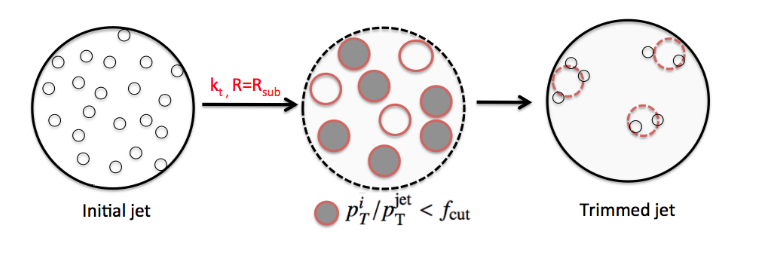
\includegraphics[width=0.9\textwidth]{jet_part/grooming/Figura_4.png}
  \caption{Schematic of the trimming algorithm.}
  \label{fig:trimming}
\end{figure}


\subsubsection{Calorimeter Mass}

% Once the collection of constituents from the large-$R$ jet is groomed, i.e. the most likely sources of soft radiation from PU and UE are eliminated, one can start working with those and start worrying about how to get physical-related properties from it, e.g. the mass.
Once the collection of constituents from the large-$R$ jet is groomed, it is possible to use them for the measure of physical related properties such as the jet mass, since the possible sources of soft radiation from PU and UE have been reduced.


The \textit{calorimeter mass} or $m^{calo}$ is a widely used variable which takes as input the topo-cluster information. Given that each topo-cluster $i$ has a 3D information on the energy deposit, $E_i$, the mass can be simply calculated from 4-vector properties:
$$m^{calo}=\sqrt{\left(\sum_{i\in J}E_i\right)^2-\left(\sum_{i\in J}p_{T,i}\right)^2} $$
where $J$ labels the Large-$R$ jet.

\subsubsection{Track Mass}
\label{sec:tracks}
% This section briefly presents the tracks and how they are related to the properties of the large-$R$ jets.
This section briefly presents the tracks and their relation with the large-$R$ jet's properties.
% There are significant advantages of tracks and why they are interesting and possible candidate for precise mass reconstruction and a big disadvantage.
There are significant advantages and few disadvantages of their usage for precise jet mass reconstruction, which are inherited both from the detector experimental properties and from the underlying physical processes. 

First of all the excellent performance of track reconstruction and angular separation at low $\pt$ is intrinsically better than the calorimeter one (see the Chapter 2. and Table \ref{tab:recap}).
The second main advantage is that tracks can be associated with the primary vertex, thus simply excluding those from PU or other beam-induced soft radiation background (this is not the case for the UE).

The requirement made on tracks to achieve optimal performance are grouped into two categories, the quality of the track, i.e. if it was fully reconstructed from the detector and separated from others with no ambiguities, and the association conditions with the primary vertex:

\begin{itemize}
 \item $p_T^{track} > 400$ MeV;
 \item $|\eta|<$ 2.5;
 \item Maximum 7 hits in the Pixel and STC sub-detectors;
 \item Maximum 1 Pixel hole;
 \item Maximum 2 silicon holes;
 \item Less than 3 shared modules;
 \item Maximum 2 mm of displacement along beam axis ($z_0$) from the primary vertex;
 \item Maximum 2.5 mm of distance in x-y plane from the primary vertex and point of closest approach ($d_0$).
\end{itemize}

Given the set of tracks which pass this selection, the mass $m^{track}$ is calculated summing up the 4-momenta of those tracks which are ghost associated to the groomed jet.

% The main, big disadvantage is that the tracker system is completely blind to the neutral component of the jet, which, as said, amounts to c.a. a third of the total. As seen in Figure \ref{fig:trackandcalo}, the track mass (red distribution) is not only shifted towards lower values than the calorimeter mass (green distribution), but its width also degrades. 

Apart from this benefits which derive from the tracker system, there is also an important disadvantage which comes from the underlying physics: it is completely blind to the electrically neutral component (mostly $\pi^0$) of the jet. As seen in Figure \ref{fig:trackandcalo}, the track mass (red distribution) is not only shifted towards lower values than the calorimeter mass (green distribution), but its width also degrades. 

\begin{figure}[!ht]
  \centering
      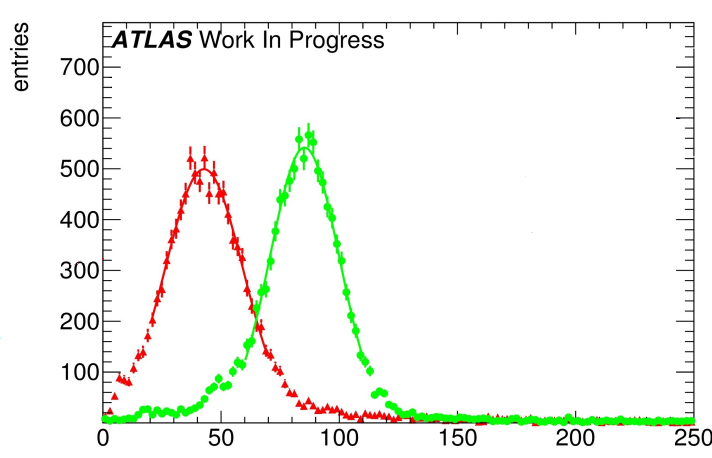
\includegraphics[width=0.7\textwidth]{jet_part/trackandcalo.png}
  \caption[Mass distribution for boosted $W/Z$]{Mass distribution boosted $W/Z$: in green the $m^{calo}$ and in red the $m^{track}$. }
  \label{fig:trackandcalo}
\end{figure}

Tracks could be used either for independent mass reconstruction (and in this section is shown how this is not the case), or, most importantly, as an ulterior information to the calorimeter measurement.

\subsubsection{Performance Figure of Merit (FoM)}
Since we already introduced the calorimeter and track mass, a concrete, quantitative feature has to be defined in order to understand which observable is ``better'', in the sense that we would prefer one or the other according to this criterion. This is often referred to as \textit{Figure of Merit} or simply FoM.

There are few ways to look at the FoM: one can e.g. na\"ively think about the mean of the mass distribution, since closer values of the mean to the e.g. $W$ or $Z$ mass (if we are speaking about $W/Z$ decays), indicate a more correct mass reconstruction. However, this does not take into account the width of this distribution, as a large width spoils the reconstruction in terms of percentage of jets misreconstructed. Moreover, the mean is not as important since it can be rescaled to the desired value in a calibration procedure.

\subsubsection{Gaussian Fit}

The important feature to keep in mind, in fact, is the underlying physics which brings us to calculate the mass of a jet. In figure \ref{fig:search} this is made clear: if the width of the invariant mass distribution of the jet is smaller (highlighted), it allows a bigger background rejection, here shown as the QCD dijet, and a higher signal efficiency, by means of a simple mass requirement.

\begin{figure}[!ht]
  \centering
      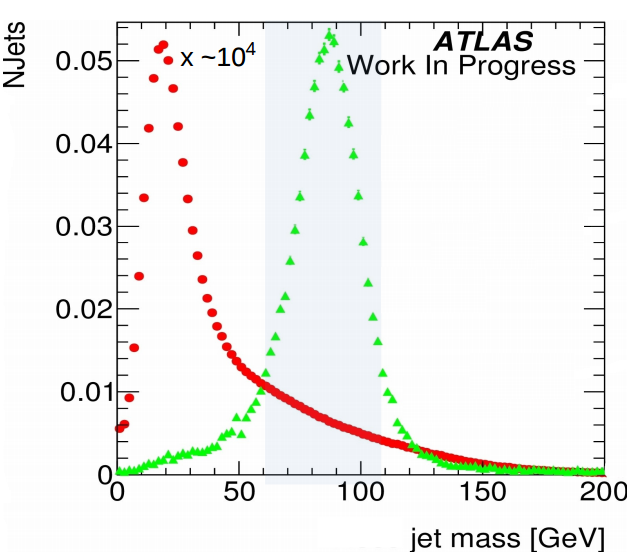
\includegraphics[width=0.55\textwidth]{jet_part/search.png}
  \caption[QCD and $W'$ mass distribution]{Mass distributions: in red the QCD dijet background rescaled, in green the $W/Z$ from the $W'$ sample. Highlighted the width of the $W/Z$ distribution.}
  \label{fig:search}
\end{figure}

The width $\sigma$ of the distribution, which can be obtained from a fit to the Gaussian core, is already a valid FoM, which has an underlying physical feature. Moreover, in order to be independent from the mean of the distribution, the width can be divided by the mean itself.
This was in fact the FoM which was used at the beginning of the work for this thesis, since it provided a simple and fast solution. However, special care must be used both in the procedure of fitting Gaussian cores of responses, since they are asymmetric, and to how the tails are treated.

\begin{figure}[!ht]
  \centering
      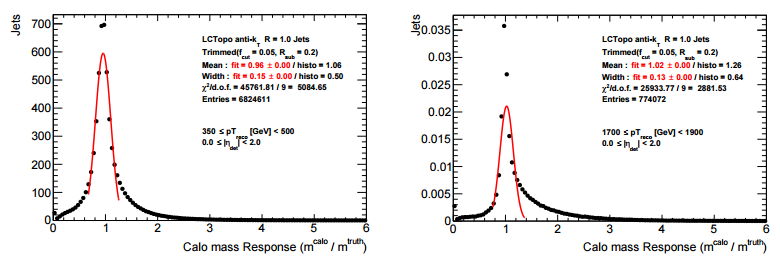
\includegraphics[width=0.9\textwidth]{jet_part/wrongsigma.png}
  \caption[Gaussian fit for QCD multijet]{Mass Response distributions for the QCD multijet for various $\pt$ ranges: on the right the failure of the Gaussian fit shows the limitation of this approach to evaluate the Figure of Merit. On the plot the fit parameters and transverse momentum ranges.}
  \label{fig:wrongsigma32}
\end{figure}

The situation is depicted e.g. in Figure \ref{fig:wrongsigma32}, where a mass response is shown for calorimeter mass for QCD multijet: here the presence of a right-handed tail which enhances going from low to high transverse momenta makes the Gaussian fit clearly not the tool which provides the stability needed. The ideal tool should take care of managing the presence of at least tails outside the Gaussian core and should converge to the intuition of the standard deviation for a perfect Gaussian distribution.
The closest tool to this idea was found to be the \textit{InterQuantile Range}, which was therefore preferred and presented in the next section.

\subsubsection{InterQuantile-Range}
Another way to look at the mass FoM is half of the 68\% of the InterQuantile range (IQnR) (here defined such as it corresponds to a sigma of a ``perfect'' Gaussian distribution: $q84\%-q16\%$ where $q84\%$ is the 84$^{th}$ percentile and $q16\%$ is the 16$^{th}$, not to be confused with the InterQua\textbf{r}tile Range (IQR) which is the $q75\%-q25\%$ and does not correspond to the sigma) divided by the Median ($\iqr$). It provides stability and high sensitivity to left-hand-side and right-hand-side tails.

Another important FoM, used for the work in this thesis, is the response distribution: given the reconstructed mass (calorimeter, track or whichever method) one can compare it to its $truth$ mass ($m^{truth}$), computed from the particle at MC level before the interaction with the detector:

$$R_m=\frac{m^{reco}}{m^{truth}}$$

Standard descriptor of the FoM e.g. in \cite{art35} and here is the IQnR of the $R_m$.
  
  
In Figure \ref{fig:iqrbin} a mass response for a single range of transverse momentum is shown, for the calorimeter mass. On the plot the contours of a standard deviation and of $q16\%$ and $q84\%$ are drawn with dashed and solid lines, respectively, showing the difference induced by the tail. This sort of plot is the key when looking quantitatively to the observable performance and can be found in the Appendix for each of the process studied in every $\pt$ range considered. In this chapter will be shown, however, the quantity which describes this FOM, the IQnR, as a function of $\pt$, in order to get an understanding of the behavior in the entire spectrum and assure the exclusion of local sub-optimalities.

\begin{figure}[!ht]
  \centering
      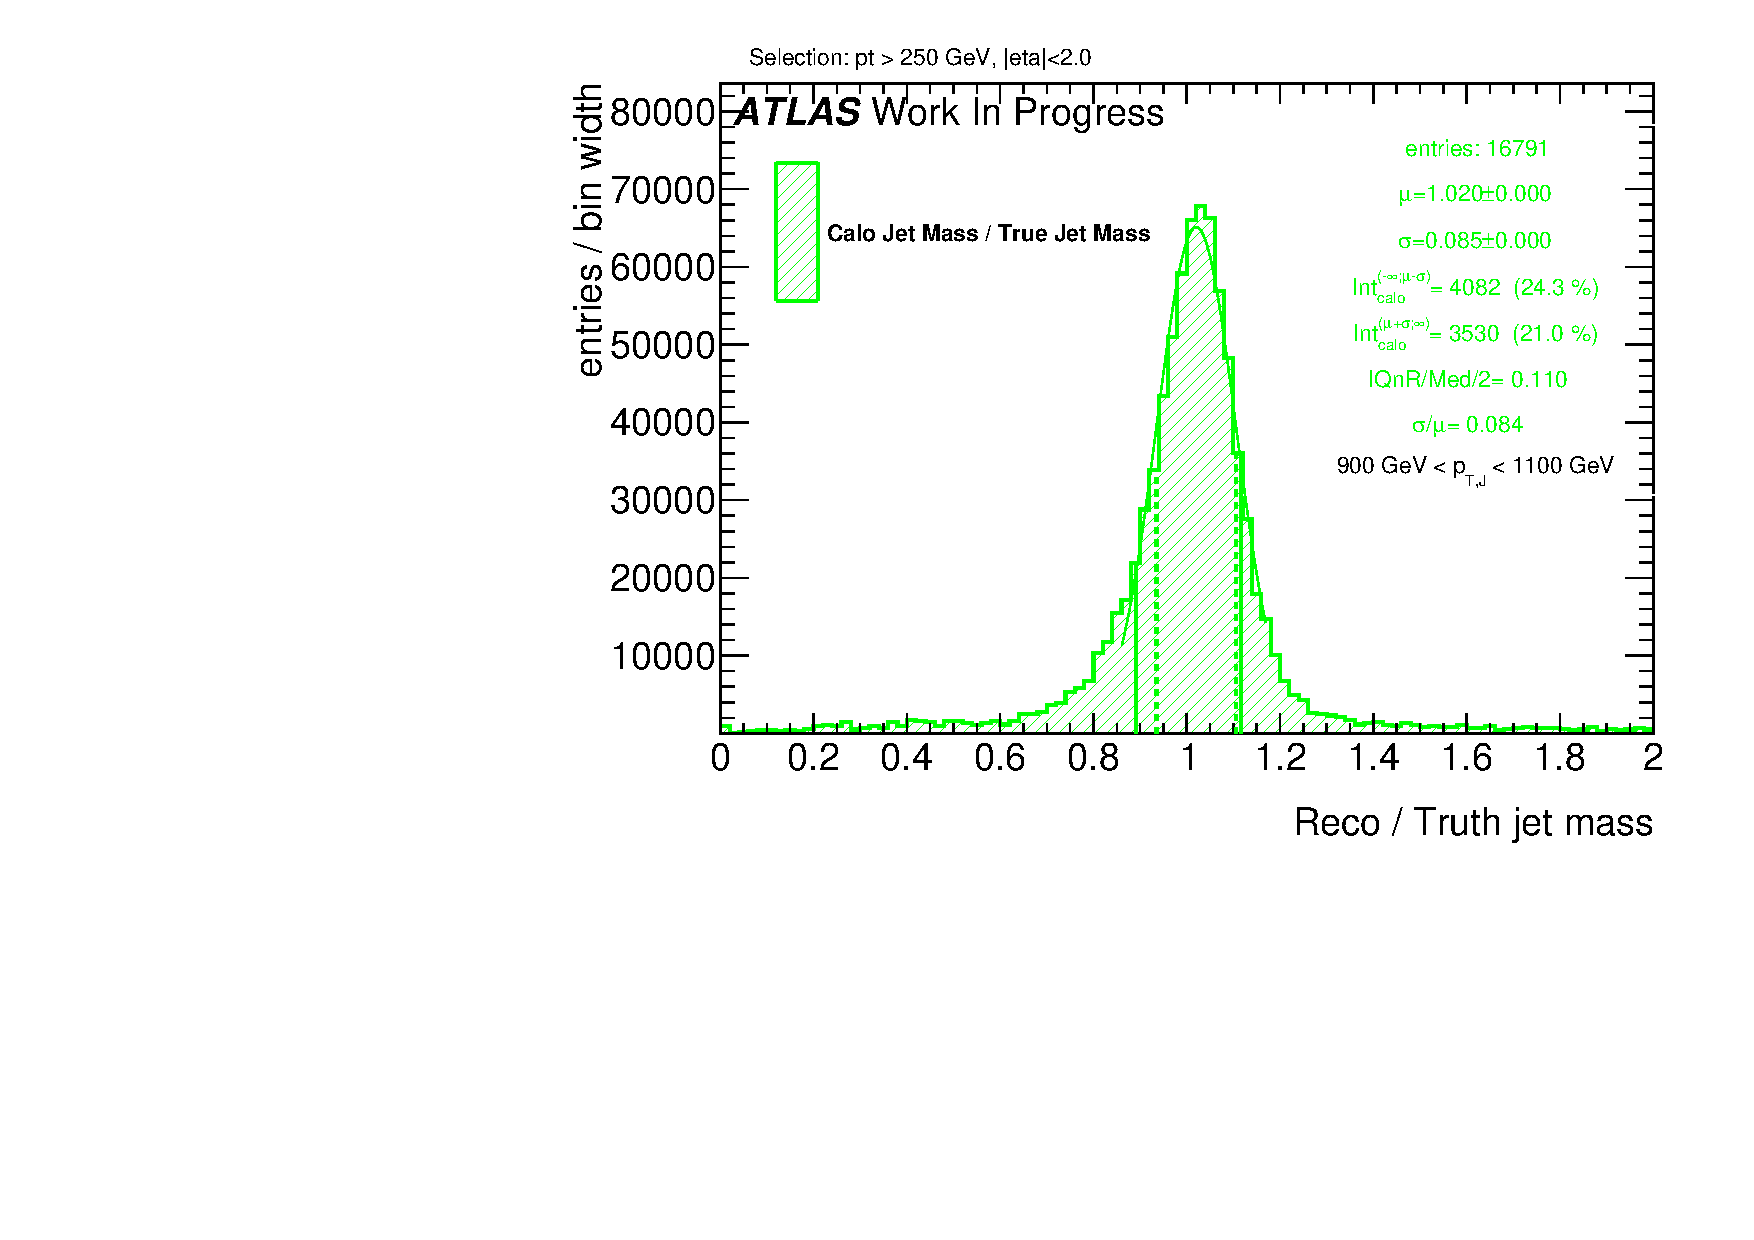
\includegraphics[width=0.7\textwidth]{jet_part/8ResponsePTJ_h_JetRatio_mJ05CALO.pdf}
  \caption[$\mcal$ response single $\pt$ bin]{Calorimeter mass response plot for boosted $W/Z$. One the plot, right, are shown: the number of entries, the mean and the width of the fit to the Gaussian core, the integral from 0 to $\mu-\sigma$ and the one from $\mu+\sigma$ to $+\infty$, the values $\iqr$ and $\sigma/\mu$. On the distribution the dashed vertical lines represent the points $\mu-\sigma$ and $\mu+\sigma$ and the solid lines represent the $q16\%$ and $q84\%$.}
  \label{fig:iqrbin}
\end{figure}


\subsection{Energy Correlation Functions}\label{subsec:ECF}
Information about the substructure of large-R jets can be used to discriminate between different event topologies. These are one, two and respectively three hard substructures (or prongs) inside the large-R jet. QCD jets are characterized by one hard substructure, jets originated by $W$ or $Z$ bosons feature two and Top quark jets feature three substructures (hadronic decay channels).

The \textsc{Energy Correlation Functions} ECF(N,$\beta$) or N-point correlators, described in Reference \cite{bib:ECF}, explore the substructure of a jet using a sum over the constituents. The correlation between pairs and triples of constituents is considered by the product of their $p_{\mathrm{T}}$, multiplied by the angular weighting, which is defined by the product of the pairwise angular distances of the considered constituents. This angular part can be scaled against the momentum part via an exponent $\beta$. The default value for $\beta$ is 1, corresponding to angular and momentum parts being weighted equally.
\begin{equation}
\begin{aligned}
 & \text{ECF1}  ={} \sum\limits_{constituents} p_{\mathrm{T}} \\ 
 & \text{ECF(2,$\beta$)} ={} \sum\limits_{i=1}^n \sum\limits_{j=i+1}^n p_{\mathrm{T},i}p_{\mathrm{T},j}\Delta R_{ij}^{\,\beta} \\ 
 & \text{(ECF(3,$\beta$)} ={} \sum\limits_{i=1}^n \sum\limits_{j=i+1}^n \sum\limits_{k=j+1}^n p_{\mathrm{T},i}p_{\mathrm{T},j}p_{\mathrm{T},k}(\Delta R_{ij} \Delta R_{ik} \Delta R_{jk})^{\,\beta}
\end{aligned}
\end{equation}\label{eq:ECF}
The ECF(N) variables can be expanded straightforwardly to larger values of N by considering this definition.
With this, ECF(2) uses pairwise correlation and is sensitive to two-prong structures, whereas ECF3 relies on triple-wise correlations to identify three-prong structures. ECF(1) corresponds to the $p_{\mathrm{T}}$ of the whole jet by a summation over the constituents $p_{\mathrm{T}}$, thereby serving as normalization to minimize the energy scale dependence.

The ECF(N) variable tends to very small values for collinear or soft configurations of $N$ constituents and is defined to be zero for jets with less than $N$ constituents. For ECF(2), only pairs of constituents that are angular separated but not soft result in sum terms that are non-negligible, which directly leads to the picture of two hard substructures inside the jet. A similar conclusion can be made for ECF(3) and three hard substructures. 
Resulting from this, a jet with $N$ or more hard substructures features a high ECFN value while a jet with fewer than $N$ substructures has a lower ECF(N) value. Consequently, one can define ratios of Energy Correlation Functions. Two of them, called C2 and D2 are found to be very powerful to distinguish between one- and two-prong like jets, see e.g. Reference \cite{bib:power_counting}. 
\begin{equation}
\begin{aligned}
 & \text{C2} ={} \frac{\text{ECF(3)}\cdot\text{ECF(1)}}{\text{ECF(2)}^2} \\ 
 & \text{D2} ={} \frac{\text{ECF(3)}\cdot\text{ECF(1)}^3}{\text{ECF(2)}^3}
\end{aligned}
\end{equation}\label{eq:C2D2} 
E.g. a jet originated from a $W$ boson features a small ECF(3) but a high ECF(2) value resulting in small C2/D2, corresponding to a high agreement with the two-prong hypothesis. QCD jets feature a very small ECF(3) and a small ECF(2) value. This results, considering the power of ECF(2) in the definitions, in a higher C2/D2 value as for a $W$ boson jet. 
These variables are IRC-safe for $\beta > 0$ and theoretically very well understood, see Reference \cite{bib:analytic_ECF}. D2 was found to perform slightly better for tagging $W$ boson jets as C2 in Reference \cite{bib:w_tagging}, most notably due to a more $p_{\mathrm{T}}$ robust cut value and a somewhat higher background rejection. 

% Stress default constituents are calorimeter clusters

\subsection{n-Subjettiness}\label{subsec:nSub}

The n-Subjettiness variable $\tau_N$, introduced in Reference \cite{bib:nsub}, quantifies the level of agreement between a given large-R jet and a certain number $N$ of sub-jet axes. Several possibilities to define the sub-jet axes exist. Two often used definitions are $k_\mathrm{T}$-axes and the $k_\mathrm{T}$-WTA (Winner Takes All) definition. In both cases, the jet is reclustered with an exclusive $k_\mathrm{T}$-algorithm, that is running the recombination just until $N$ sub-jets are clustered. The $k_\mathrm{T}$-axes are defined by the four-momenta of the $k_\mathrm{T}$-sub-jets, WTA correspond to the four-momentum of the hardest constituent in each $k_\mathrm{T}$-sub-jet. Used in this study is th $k_\mathrm{T}$-WTA axis definition. 

As C2 and D2, N-Subjettiness is a measure for the whole jet, calculated via a sum over the jets constituents (calorimeter clusters as default).
\begin{equation}
\tau_N = \frac{1}{d_0}\sum_k p_{T,k}\:min(\Delta R_{1,k},\Delta R_{2,k},...,\Delta R_{N,k})^{\beta}
\end{equation}

For each term, the constituents $p_{\mathrm{T}}$ is multiplied by the distance to the nearest sub-jet axes. The overall value is normalized with a sum over the constituents $p_{\mathrm{T}}$ times the characteristic radius parameter $R$ of the large jet.
\begin{equation}
d_0=\sum_k p_{T,k}R_0
\end{equation}
Similar to ECF(N,$\beta$), the angular measure $\Delta R_{ij}$ can be scaled relative to the $p_{\mathrm{T}}$ factor via the exponent $\beta$. N-Subjettiness is an IRC-safe variable for values of $\beta \ge 0$.

Small values of $\tau_N$ correspond to a jet with all constituents more or less aligned or near to the given $N$ sub-jet axes, hence the jet is compatible with the assumption to be composed of $N$ or fewer sub-jets. A higher value in contrast indicates a consistency with more than $N$ sub-jets as a non negligible part is located apart of the $N$ sub-jet axes. Consequently, $W/Z$ or Higgs boson jets are likely to feature a small $\tau_2$ and a high $\tau_1$ value. QCD jets with their one-prong structure result in a high $\tau_{2}$ and a small $\tau_{1}$ value. While $\tau_1$ and $\tau_2$ alone provide only slightly separation, the ratio 
\begin{equation}
\tau_{21} = \frac{\tau_2}{\tau_1}  
\end{equation}
is an effective discrimination variable.

The extension to three-prong like jet identification and discrimination from one and two-prong structures follows quite naturally by taking the ratio of $\tau_3$ and $\tau_2$.
\begin{equation}
\tau_{32} = \frac{\tau_3}{\tau_2}  
\end{equation} \\
Consequently, the hadronic decay of top quarks via $t \rightarrow Wb$ and the $W$ decaying into two quarks can be tagged using the $\tau_{32}$ variable.


\subsection{Receiver Operator Characteristics}\label{sec:ROC}
The separation power of discrimination variables can be studied quite intuitively by comparing the signal and background distributions of a certain variable. Another used figure of merit for the performance, especially for comparisons of different variables, is to use \textsc{Receiver Operator Characteristics} (ROCs) which show the achieved background rejection for different values of signal efficiency (signal fraction left after performing a cut). 
Each point is calculated from the underlying signal and background distributions by integrating the background distribution from zero \footnote[1]{If the signal distribution lies at lower values as the background.} to the point where the desired signal fraction is achieved. The fraction of background events contained in this region are kept when cutting at this signal efficiency, hence the inverse of this fraction, $\frac{1}{\epsilon_{background}}$ is an estimate for the background rejection. The lower the fraction of background events in the region, the better is the achieved exclusion. Accordingly, a good discrimination variable is represented by a ROC with preferably high values of background rejection up to high signal efficiencies.



%-------------------------------------------------------------------------------
\section{Track-assisted subjet mass}
\label{sec:mtas}
%-------------------------------------------------------------------------------
The track-assisted subjet mass takes inspiration from the simpler development which is already implemented within ATLAS, the track-assisted mass which is described briefly below for completeness.


\subsection{Track-Assisted Mass ($\mta$)}\label{subsec:mta}
The main limitation of the calorimeter mass comes from the angular resolution of the topo-clusters, which, for extreme kinematic regimes, start approaching each other at the point that they hit the granularity of the detector. The main advantage is that on the contrary the relative energy resolution increases at higher energies.

The tracks instead have a very good angular resolution, but $\pt$ relative resolution degrades linearly with the transverse momentum. 

One could then think about creating a variable which exploits the advantages of both and minimizes the disadvantages. As seen, the track mass is missing the neutral component, i.e. each measurement is missing the fraction $\frac{neutral+charged}{charged}$, but it could be corrected on a jet-by-jet basis: this leads to the definition of the \textit{track-assisted mass} ($m^{TA}$):
\begin{equation}
 m^{TA}=\frac{p_T^{calo}}{p_T^{track}}\times m^{track}
\end{equation}

It can be intuitively understood as follows: the term $m^{track}$ has the superior angular resolution, but misses the neutral component; the ratio $p_T^{calo}/p_T^{track}$, representing exactly the $(neutral+charged)/charged$ ratio, ``restores'' the correct value of the mass back to $charged+neutral$.
\begin{figure}[!ht]
  \centering
      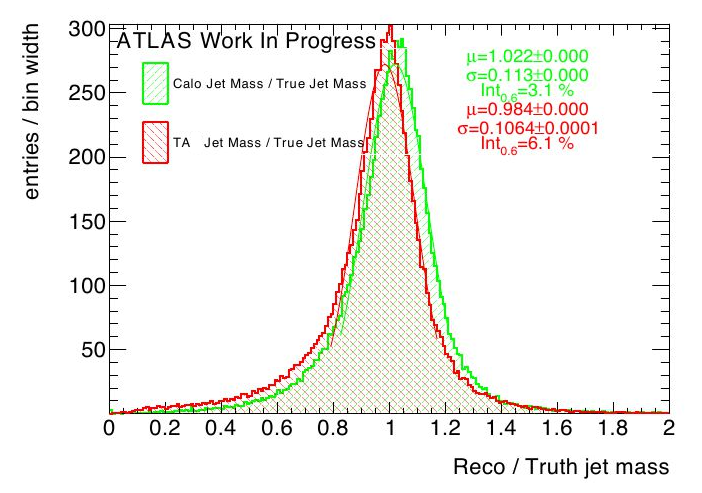
\includegraphics[width=0.7\textwidth]{jet_part/mta/allbinptmta.png}
  \caption[$\mcal$ and $\mta$ mass responses]{Track-assisted mass response plot for boosted $W/Z$: in green the calorimeter mass, in red the track-assisted mass. On the right are shown properties of the fit to the Gaussian core; it can be seen than the width of the $\mta$ distribution is smaller, and the mean is slightly below the calorimeter mass.}
  \label{fig:mta1}
\end{figure}

From Figure \ref{fig:mta1} the comparison of the track-assisted mass and the calorimeter mass; the width of the distribution is smaller, making this observable a good candidate for usage.


\subsection{Advantages and Limitation of $\mta$}
The $\mta$ has a good handle on boosted $W/Z$, looking at all the transverse momentum spectrum for these results.

\begin{figure}[!ht]
  \centering
      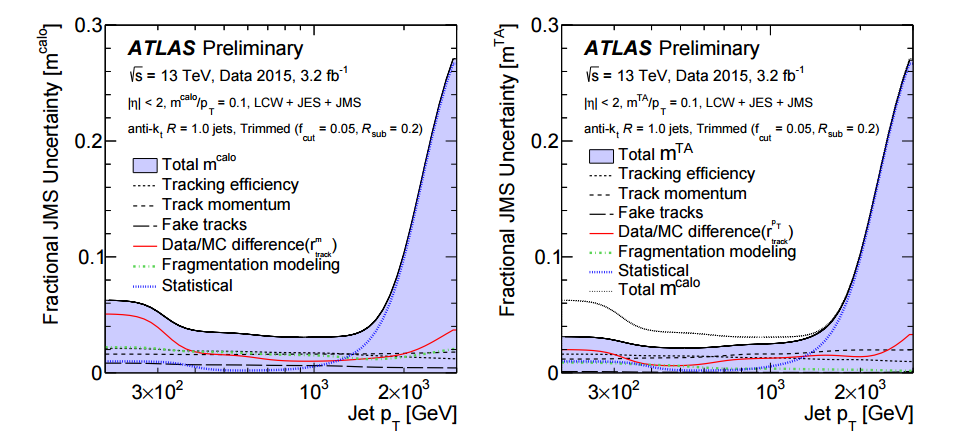
\includegraphics[width=0.9\textwidth]{jet_part/uncert.png}
  \caption[Comparison of the uncertainties for $\mcal$ and $\mta$]{Comparison of the uncertainties for $\mcal$, on the left, and $\mta$, on the right the rise on the high jet $\pt$ is due to statistics. From the \cite{art35}.}
  \label{fig:uncert}
\end{figure}

Another big advantage which supports the use of the track-assisted mass is the relatively small uncertainties: in Figure \ref{fig:uncert} the comparison of $\mcal$ (left) and $\mta$ (right) fractional uncertainties on the JMS, shows how the tracking uncertainties are much smaller because of the ratio $m^{track}/p_T^{track}$. On the right plot the black line indicates the JMS fractional uncertainty for the $\mcal$, and is always above the $\mta$. Of course this introduces another argument in the development of new techniques, which is to look for a good balance between performance and small uncertainties: a perfect observable in terms of behavior which has very big uncertainties is not really useful.


When looking in the extreme kinematic regime, at very high $\pt$, as in the top plot in Figure \ref{fig:mta2}, the $\mta$ shows its real strength, achieving much smaller value of the IQnR.
However, there are some severe limitations which are worth noting, especially looking at the performance in different regions of transverse momentum: this is shown in the bottom plot of Figure \ref{fig:mta2}, where at a low $\pt$ it exhibits a much worse behavior.

\subsubsection{Performance in $W \to q'\bar{q}$ Decays}

\begin{figure}
    \centering
    \begin{subfigure}[b]{0.5\textwidth}
	\centering
        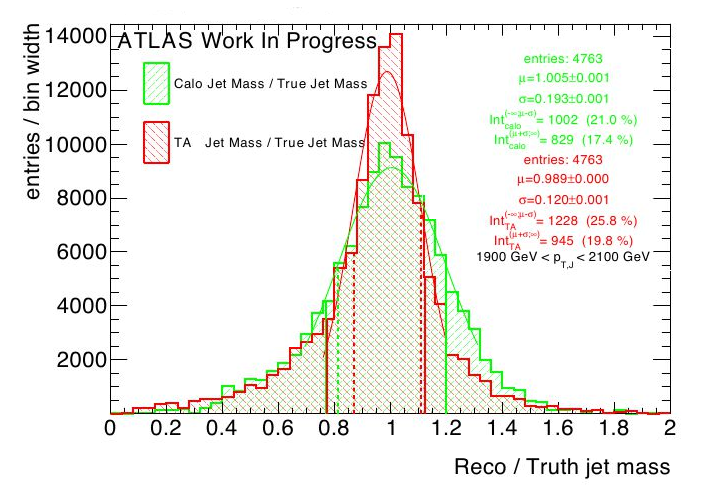
\includegraphics[width=\textwidth]{jet_part/mta/highptmta.png}
   
%         \label{fig:tiger}
    \end{subfigure}
    \begin{subfigure}[b]{0.5\textwidth}
	\centering
        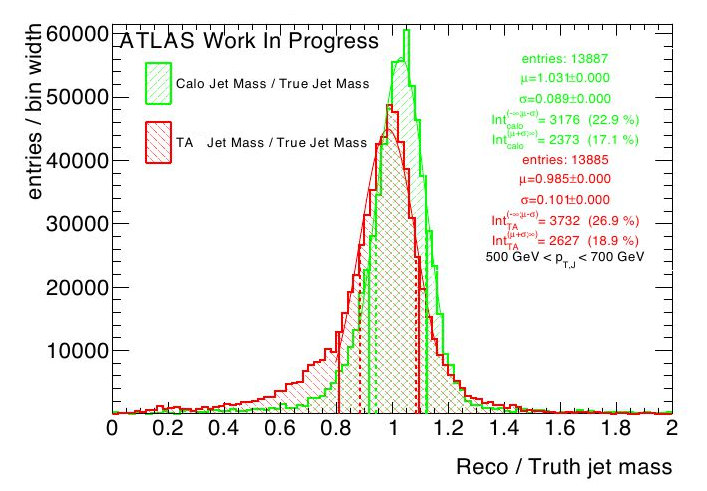
\includegraphics[width=\textwidth]{jet_part/mta/lowptmta.png}
 
%         \label{fig:gull}
    \end{subfigure}
    \caption[Mass response plots for the $\mta$]{Mass response plots for selected ranges of $\pt$: on the bottom, a ``low'' range, 500 GeV $<\pt<$ 700 GeV, on the top an high $\pt$, 1900 GeV $<\pt<$ 2100 GeV. A difference in performance can be clearly seen.} 
    \label{fig:mta2}
\end{figure}


The performance in all the bins of $\pt$ can be studied looking at Figure \ref{fig:mta3}; these plots have as horizontal axis the transverse momentum and as vertical one the value of the $\iqr$ calculated from the correspondingly response. For $W/Z$ jets, there is a crossing point around $\pt\sim$1 TeV, which can be understood as the point in which the two sub-jet present start merging (sub-jet multiplicity shown in Figure \ref{fig:multi} in Appendix).



\subsubsection{Performance in $t\to q'\bar{q}b$ Decays}

For top quarks the situation is much different: with respect to $W/Z$ jets, in fact, there are two main disparities: on one side, the mass of the top quark is much higher than the one of the electroweak bosons, hence making the separation $\Delta R=\frac{2m}{\pt}$ bigger; on the other side, the decay is not anymore two-prong (two-sub-jet-like) but rather a three-prong  (three-sub-jet-like) decay, one from the b-jet and the other two from the $W$ decay.
$\mta$ is here never performing better than $\mcal$, as can be seen e.g. in Figure \ref{fig:mta3}, right.


\begin{figure}[!ht]
  \centering
      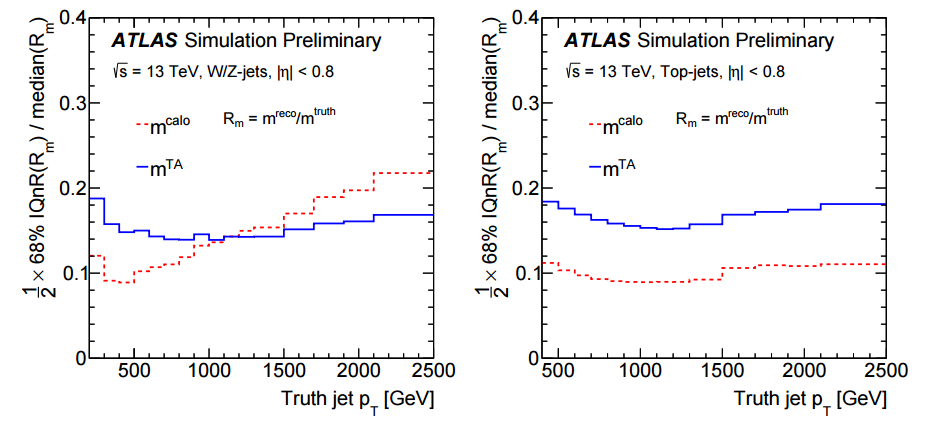
\includegraphics[width=\textwidth]{jet_part/mtawandtop.png}
  \caption[$m^{calo}$ and $m^{TA}$ comparison for $W/Z$ jets and top jets]{The comparison between the performance of $m^{calo}$ and $m^{TA}$ for $W/Z$ jets (left) and top jets (right); on the x-axis the transverse momentum and on the y-axes the $\iqr$ of the mass distribution, from \cite{art35}. A better observable has lower values on the y-axis. }
  \label{fig:mta3}
\end{figure}

\subsubsection{Performance in $h\to b\bar{b}$ Decays}

For boosted Higgs the $\mcal$ outperforms the $\mta$ in the spectrum of transverse momentum. Although the decay is two-pronged, the mass of the Higgs is higher than the electroweak bosons, moreover another difference lays in light quarks initiated jets and heavy quarks initiated ones, like the b-quarks from Higgs decay.
% the b-jet poses an additional complication which comes from the branching ratio of B mesons to muons, which leave very little energy in the calorimeter system but additional tracks.

\begin{figure}[!ht]
  \centering
      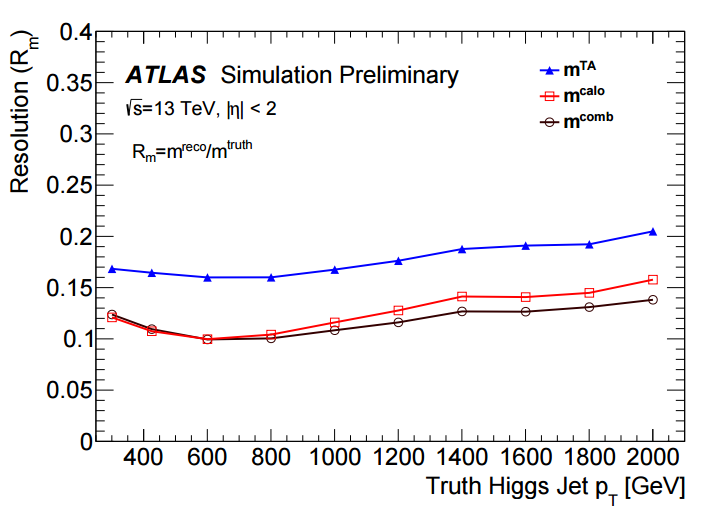
\includegraphics[width=0.7\textwidth]{jet_part/mta/higgsmta.png}
  \caption[Performance of the $\mta$ with the boosted Higgs sample]{Performance of the $\mta$ with the boosted Higgs sample; the $\mta$ is the blue line, the $\mcomb$ will be described later in this chapter. From \cite{art39}. The FoM here is the resolution of the Response.}
  \label{fig:mta4}
\end{figure}



\subsection{The Track-Assisted Sub-jet Mass ($\mtas$)}\label{subsec:mtas}
In this section the main outcome of the work of this thesis is presented: the \textit{track-assisted sub-jet mass} ($\mtas$).
The main idea takes inspiration from the track-assisted mass: if one can use the tracks to exploit the better angular resolution and correct the missing neutral component jet-by-jet, there is an additional information that can be used. The neutral fraction, in fact, varies stochastically not only per-jet basis, but even per-sub-jet basis, since each sub-jet is originated from a different quark.
Correcting the missed neutral component per-sub-jet, it should perform better already at an intuitive level, as it accesses information from the jet substructure.
There are few question in the definition of this mass observable, whose answers are in the next section:
\begin{itemize}
  \item Regarding the inputs:
  \begin{itemize}
     \item How to select the set of tracks to be used?
     \item Which kind of sub-jet should be used?
  \end{itemize}
  \item Regarding the procedure
  \begin{itemize}
  
  \item How to associate the tracks to a sub-jet?
  \item How to correct for the missed neutrals on a sub-jet basis?
  \item How to add everything back together?
 \end{itemize} 
 
\end{itemize}

Those details are given in the next subsection.


\subsection{Observable Definition: Inputs}
There are two inputs to the $\mtas$: the tracks and the sub-jets. The definition of the standard inputs are give here; alternative approaches are given in subsection \ref{sec:alternate}.

\subsubsection{Tracks}
Only the tracks that satisfy the quality criteria and primary vertex association, described in the previous section \ref{sec:tracks}, are used.
The tracks taken additionally are required to be ghost associated to the sub-jets of the groomed jet; namely only the sub-jets which survived the trimming procedure and are described in the next subsection.
Ghost association provides a one-to-one correspondence to the sub-jets set, and was therefore chosen and preferred to other kind of assignments.

\subsubsection{Sub-jets}

The choice of sub-jets must follow a simple requirement: of course we want to take those which most likely come from the hard-scattering. This means that the choice of taking them after grooming is forced.

As grooming technique used, the trimming was preferred as being the standard in ATLAS and the most flexible one for optimization studies.

The standard version of the trimming uses the k$_t$ reclustering algorithm with radius of 0.2, with the transverse momentum ratio $f_{cut}$ at 5\%.

As shown later, this is also the optimal configuration for sub-jets.

\subsection{Observable Definition: Procedure}\label{subsec:ObsDef_Proc}
Having tracks and sub-jets now well defined, we can describe the recipe to produce the $\mtas$. For brevity we will call the sub-jets SJ in the formulae below. 

As said, the tracks are the one ghost-associated to the sub-jets; however, tracks which fall inside the area of the large-$R$ jet, but not inside the sub-jets area, are still much probably coming from the hard-scattering. They are then associated again to the closest sub-jets via $\Delta R$ association.

Each sub-jet will have at this point some tracks associated via ghost-association and some other via $\Delta R$ (which are maximally 5\%). We call this set of tracks, a ``custom'' Track-Jet or TJ.

At this point, the one-to-one correspondence is still preserved (for each SJ there is one and only one TJ), and we can move on correcting the neutral fraction.

Getting inspired from the formula $m^{TA}=p_T^{calo}/p_T^{track}\times m^{track}$, we would like to replicate this at sub-jet level, i.e.

$$\mtas="\sum_{SJ}"\frac{p_T^{SJ}}{p_T^{TJ}}\times m^{TJ}$$

Since now we are working inside the sub-jets we need to change the sub-jet's 4-vector itself and not only the mass: if we call $p_\mu^{TJ}$ the Lorentz vector of the track-jet, 

$$p_\mu^{TJ} = \spvec{m^{TJ};p_T^{TJ};\eta^{TJ};\phi^{TJ}} \to p_\mu^{TA}=\spvec{m^{TJ}\times\frac{p_T^{SJ}}{p_T^{TJ}} ;p_T^{SJ};\eta^{TJ};\phi^{TJ}} $$
 
where $p_\mu^{TA}$ is the track-assisted sub-jet's 4-vector. If we label $i$ the $i$-th track-jet of the $N$ ones present in the large-$R$ jet,

$$ \mtas=\sqrt{\left(\sum_i^N p^{TA} \right)_\mu \left(\sum_i^N p^{TA} \right)^{_\mu}} $$
 
\begin{figure}[!ht]
  \centering
      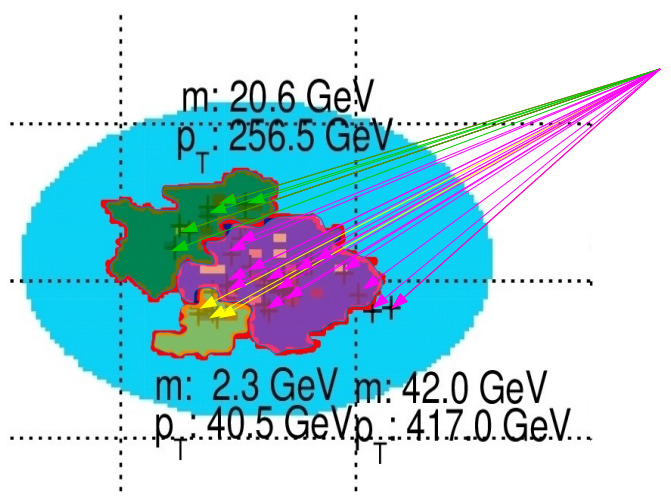
\includegraphics[width=0.6\textwidth]{jet_part/mtas/mtas.png}
  \caption[Pictorial event display]{Pictorial event display showing the $\eta$ $\phi$ region of a large-$R$ jet, (in blue the catchment area of the anti-k$_t$) showing the different k$_t$ sub-jets: they are highlighted in green, fuchsia and yellow. The associated track-jets (here as arrows pointing the calorimeter area) are colored with the same color of the correspondent sub-jet. Some tracks associated with $\Delta R$ procedure can be seen in the fuchsia sub-jet. The transverse momenta and mass values are also shown for the sub-jets.}
  \label{fig:mtas1}
\end{figure}

An important remark is that, in the case of a large-$R$ jet with only one sub-jet, the $\mtas$ has exactly the same definition of the $\mta$. This implies, since the angular separation of the decay product scales inversely with $\pt$, that the performance should approach the one of the $\mta$ in the extreme kinematic regime. However, the space for improvement is precisely in the low-middle $\pt$ regime, as seen in the $\mta$ section.

\subsection{Performance in $W \to q'\bar{q}$ Decays}
The boosted $W/Z$ was the first one looked at, and with which the $\mtas$ was designed. The $\mcal$ shows a fast deterioration of the performance at high $\pt$, and, as shown in the previous section, the $\mta$ prevents this deterioration but suffers at low transverse momenta ($\pt<1$ TeV).
The $\mtas$ has the same behavior in the extreme transverse momentum regime as the $\mta$, since the sub-jet multiplicity peaks at one, where there are no differences between the two observables.
In the low-$\pt$ regime, on the contrary, it exploits the different charged to neutral fluctuation, achieving a better performance.
This is shown in Figure \ref{fig:mtas2} as a function of $\pt$: below $\sim$ 1 TeV ic achieves lower values of the IQnR converging from below to the $\mta$ as the number of sub-jets decreases to one.

\begin{figure}[!ht]
  \centering
      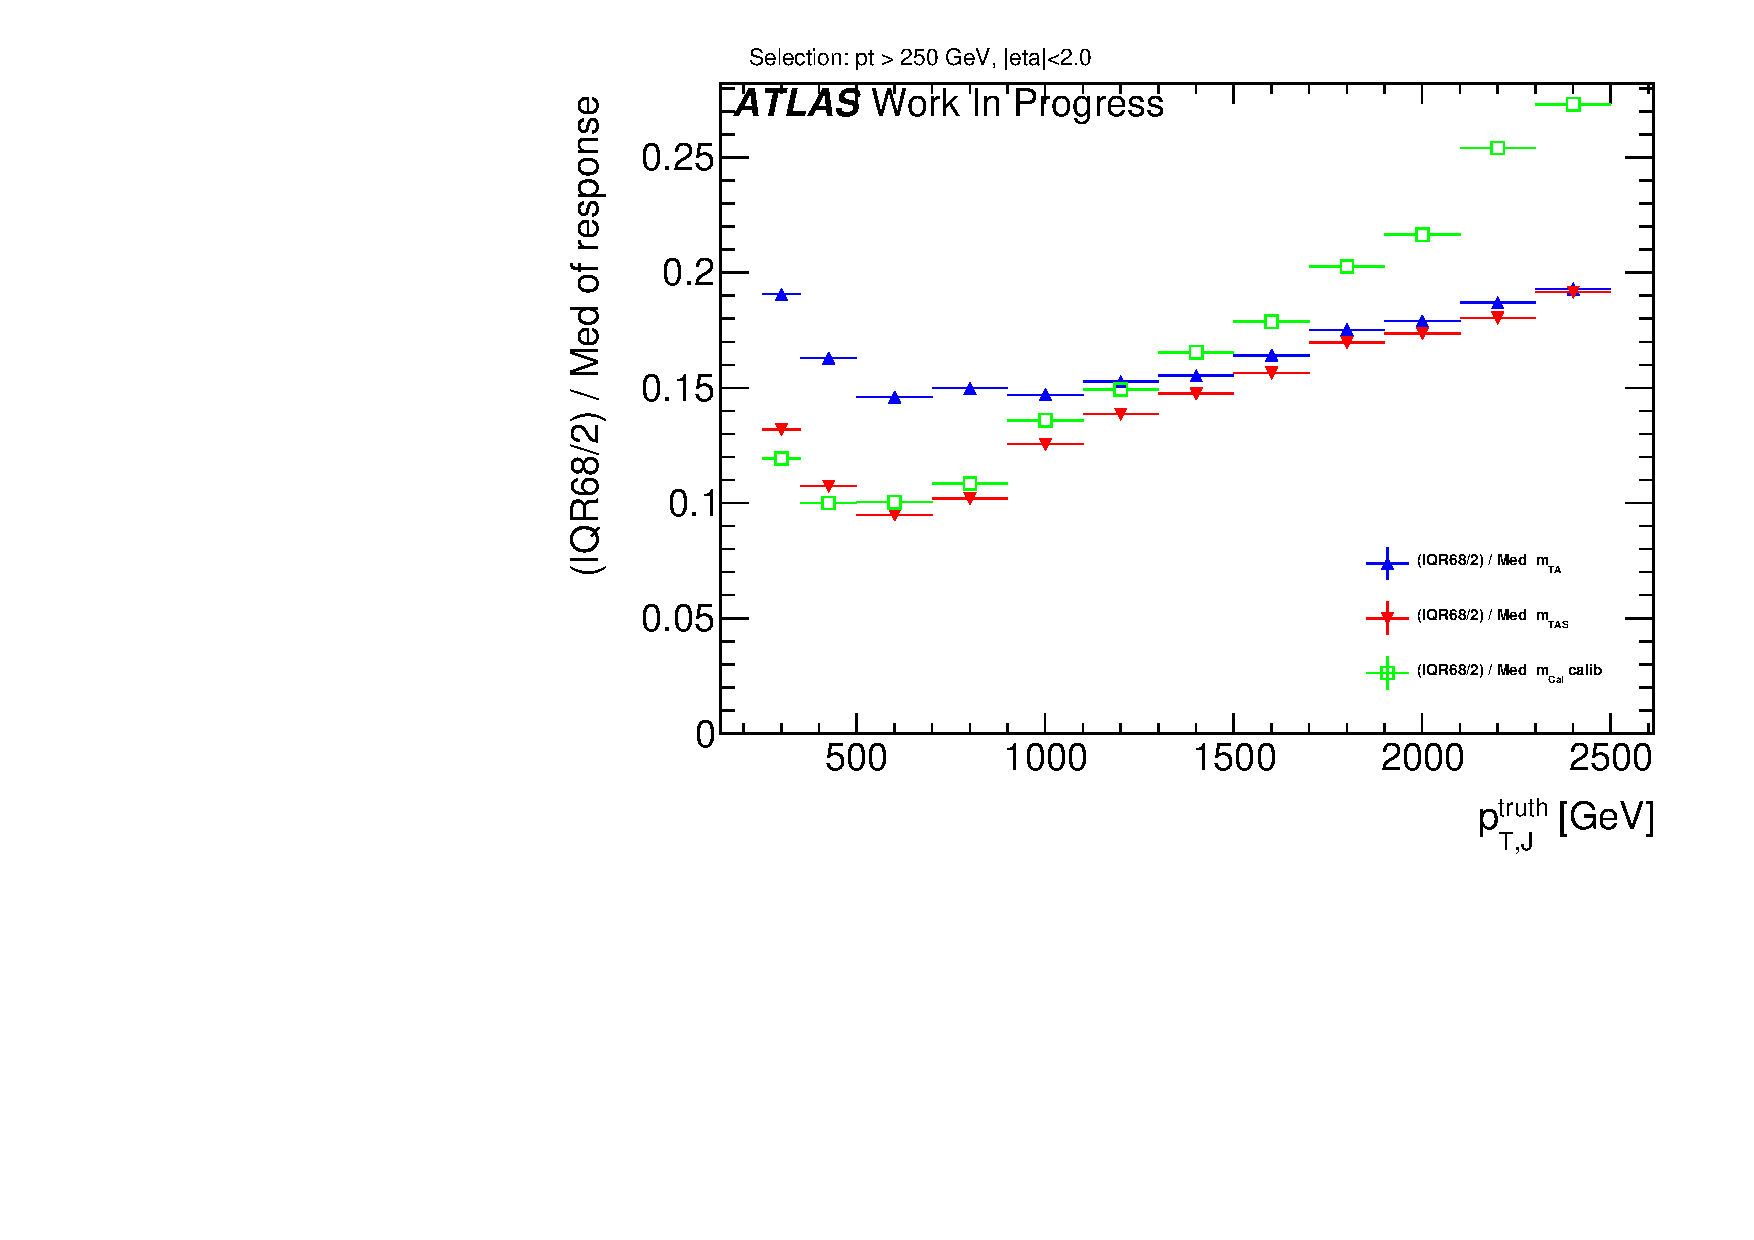
\includegraphics[width=0.7\textwidth]{jet_part/mtas/71graphcftr_h_JetRatio_mJ12CALOIQRoMWZ.pdf}
  \caption[$\mtas$ for boosted $W/Z$]{Performance of the $\mtas$ versus the $\mcal$ and $\mta$ for the boosted $W/Z$ sample.}
  \label{fig:mtas2}
\end{figure}

\subsection{Performance in $t\to q'\bar{q}b$ Decays}
The boosted tops are shown on Figure \ref{fig:mtas3}; the $\mtas$ is comparable yet slightly worse than the $\mcal$ in the low-middle $\pt$ regime, while degrades at higher $\pt$ approaching the $\mta$, which is far beyond the track-assisted sub-jet mass in performance.
As already noted, the worse performance can be ascribed both to the higher top-quark mass, and to its different and more complex decay topology.


\begin{figure}[!ht]
  \centering
      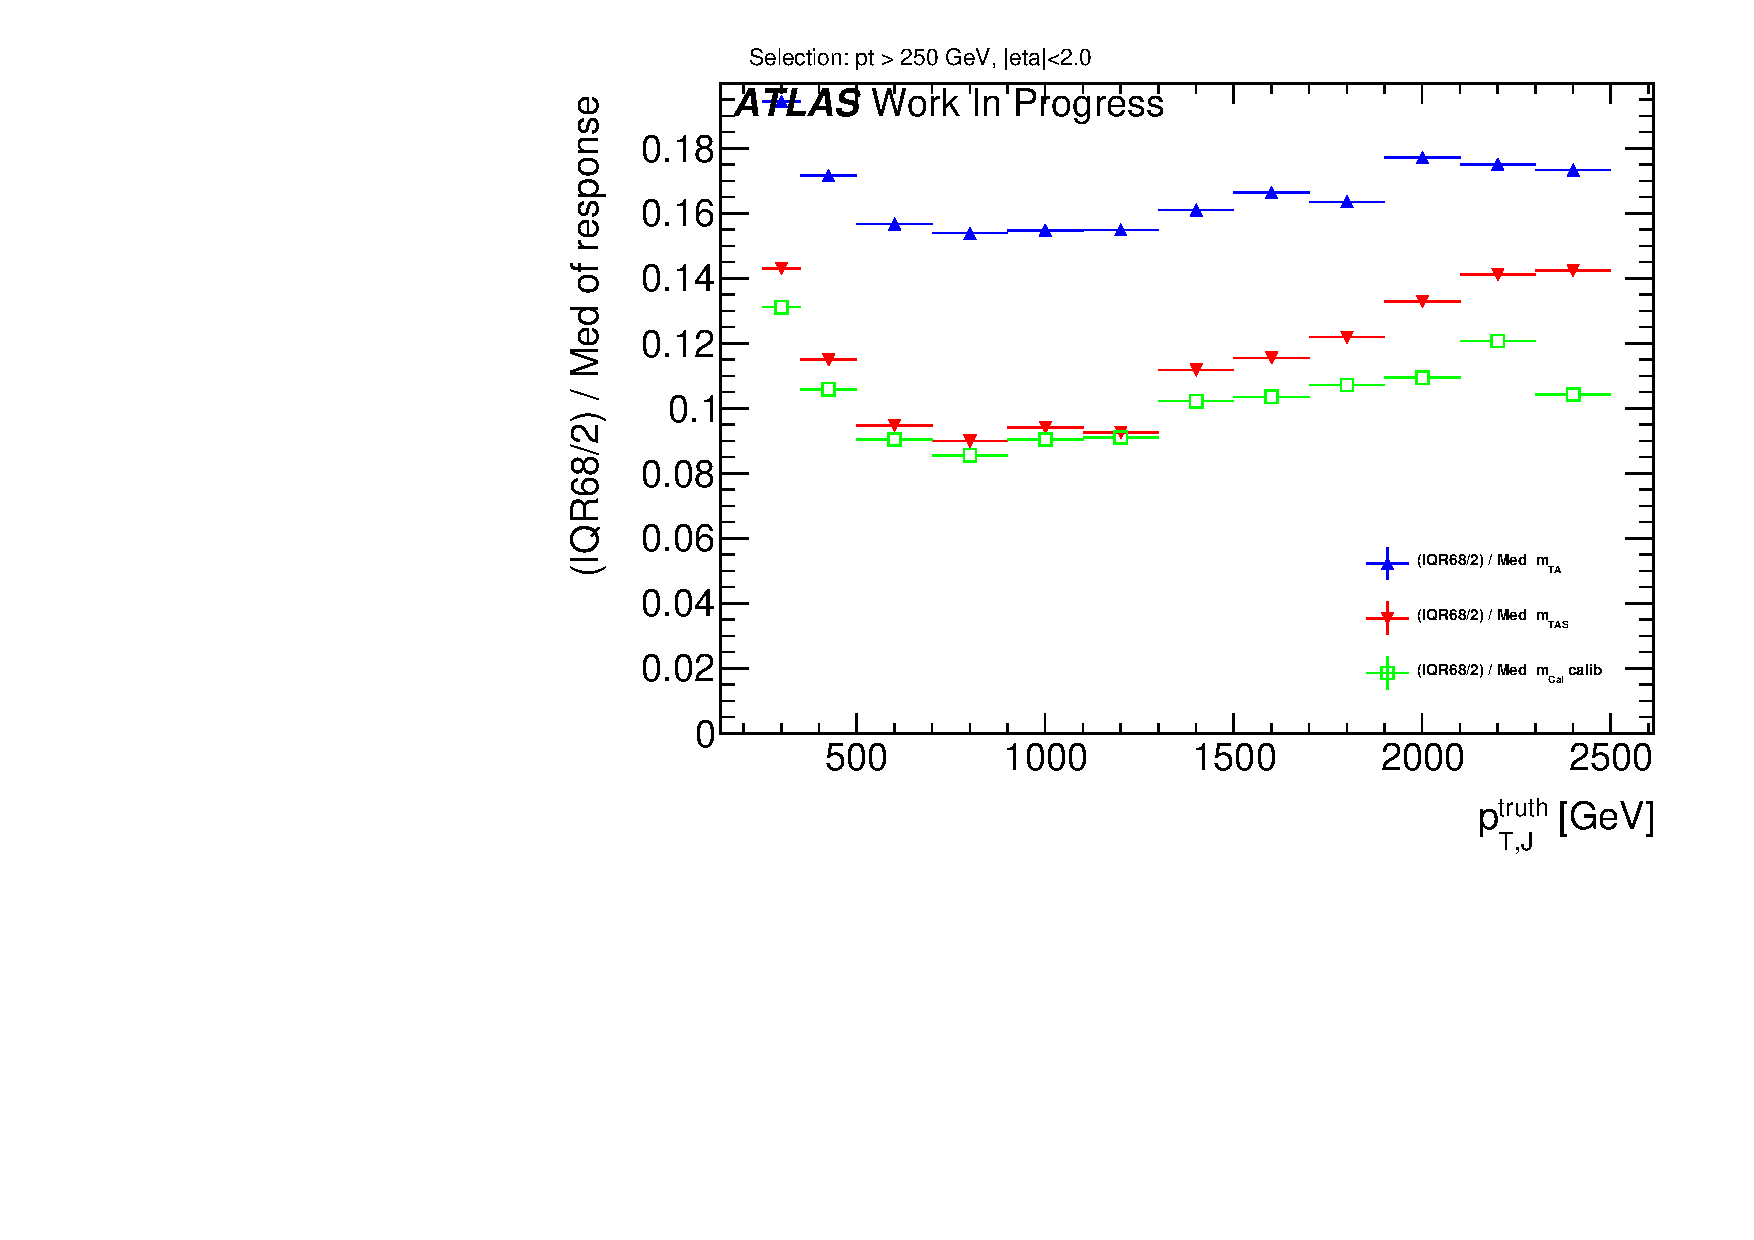
\includegraphics[width=0.7\textwidth]{jet_part/mtas/71graphcftr_h_JetRatio_mJ12CALOIQRoMTops.pdf}
  \caption[$\mtas$ for boosted tops]{Performance of the $\mtas$ versus the $\mcal$ and $\mta$ for the boosted top sample.}
  \label{fig:mtas3}
\end{figure}
\subsection{Performance in $h\to b\bar{b}$ Decays}
In the Randall-Sundrum graviton to di-Higgs to four b-quark, the performance is again problematic for the $\mta$ with respect to $\mcal$, which is far beyond the latter, while the performance of the $\mtas$ is partially similar to the boosted top-quark sample, but degrades much more in the extreme $\pt$ regime, following the $\mta$. Shown in Figure \ref{fig:mtas4}.

\begin{figure}[!ht]
  \centering
      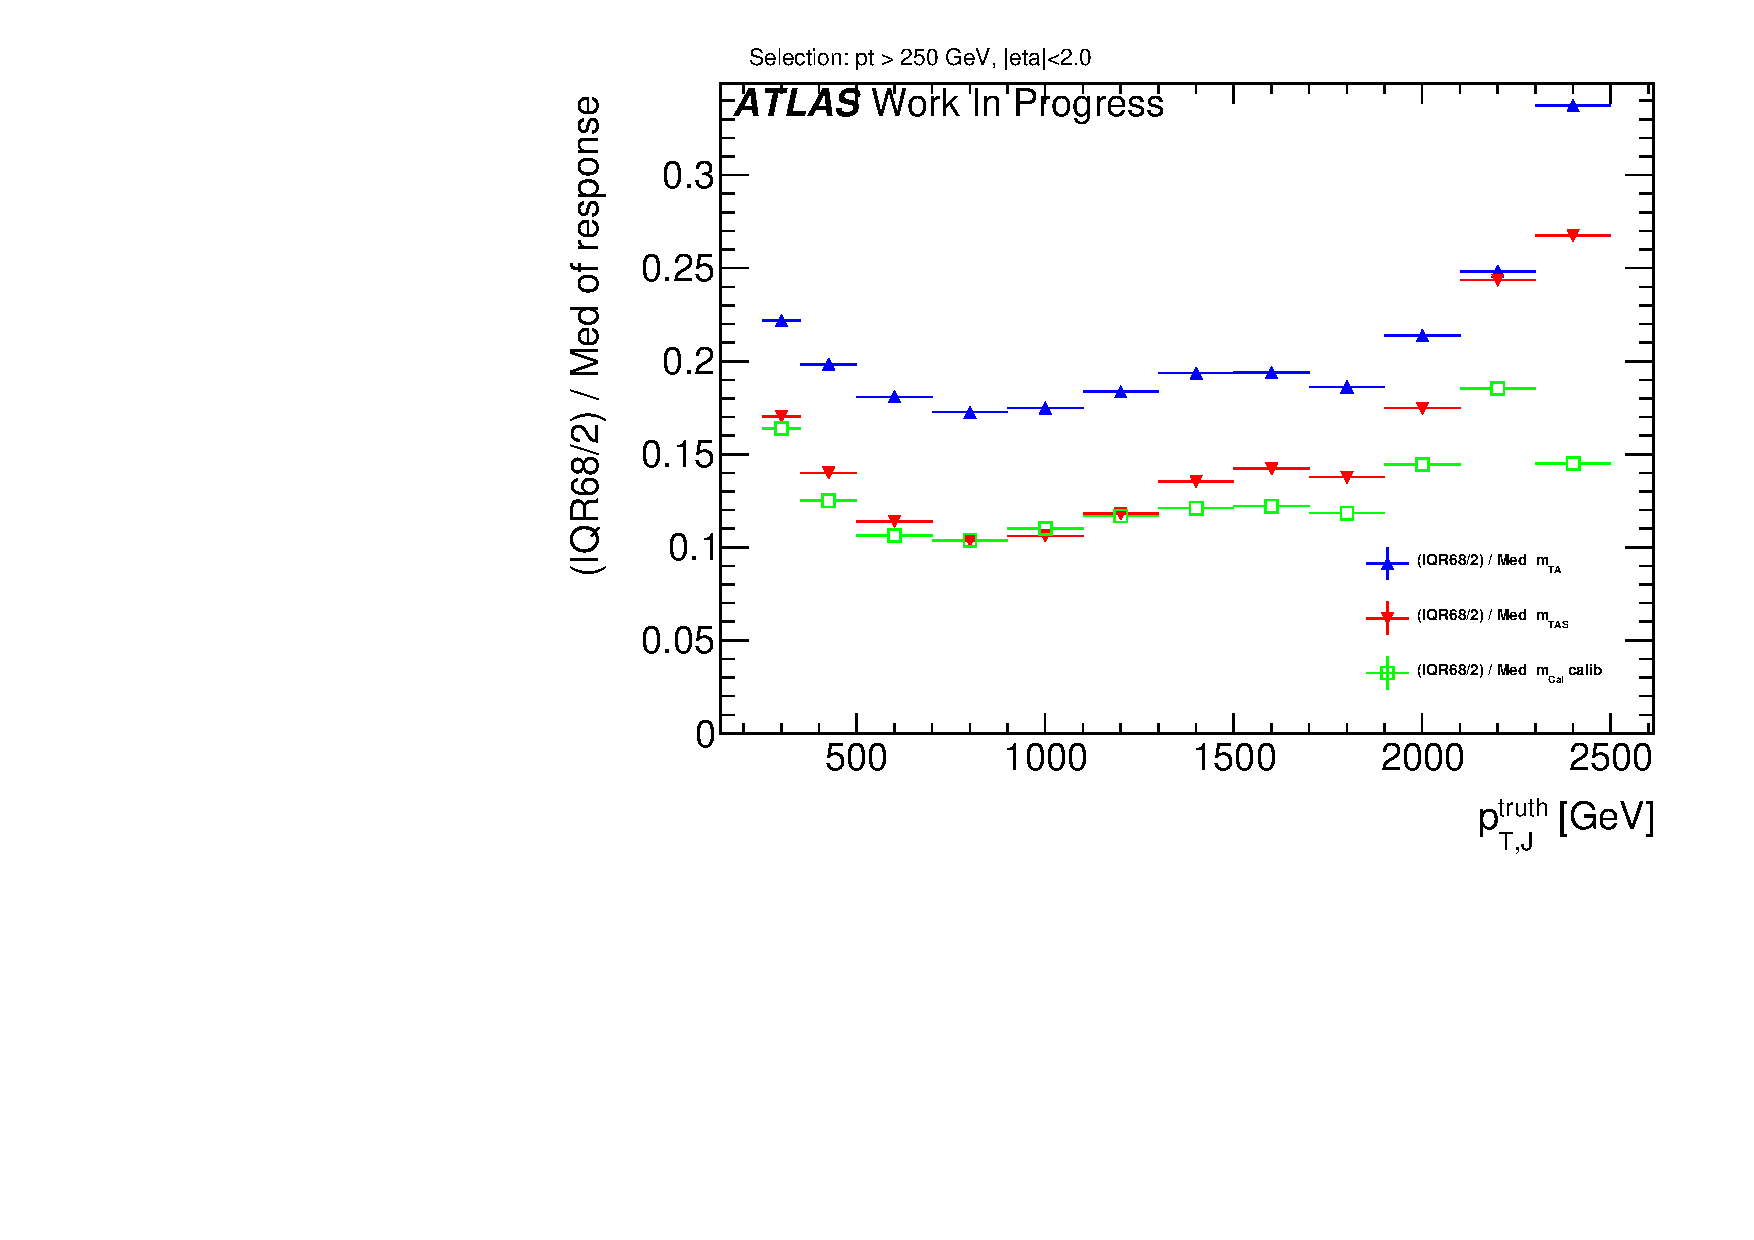
\includegraphics[width=0.7\textwidth]{jet_part/mtas/71graphcftr_h_JetRatio_mJ12CALOIQRoMHiggs.pdf}
  \caption[$\mtas$ for boosted Higgs]{Performance of the $\mtas$ versus the $\mcal$ and $\mta$ for the boosted Higgs sample.}
  \label{fig:mtas4}
\end{figure}

\subsection{Performance in QCD Multijet Events}
The behavior of the QCD multijet sample is similar to the boosted $W/Z$ sample, where the $\mta$ exhibits a crossing point in the middle-low regime $\pt\simeq900$ GeV and proceeds with a better performance at high transverse momenta.
Again the $\mtas$ follows this similarity showing no crossing point and an optimal overall behavior, both with respect to calorimeter- and track-assisted-based mass definition. On Figure \ref{fig:mtas5}.

\begin{figure}[!ht]
  \centering
%       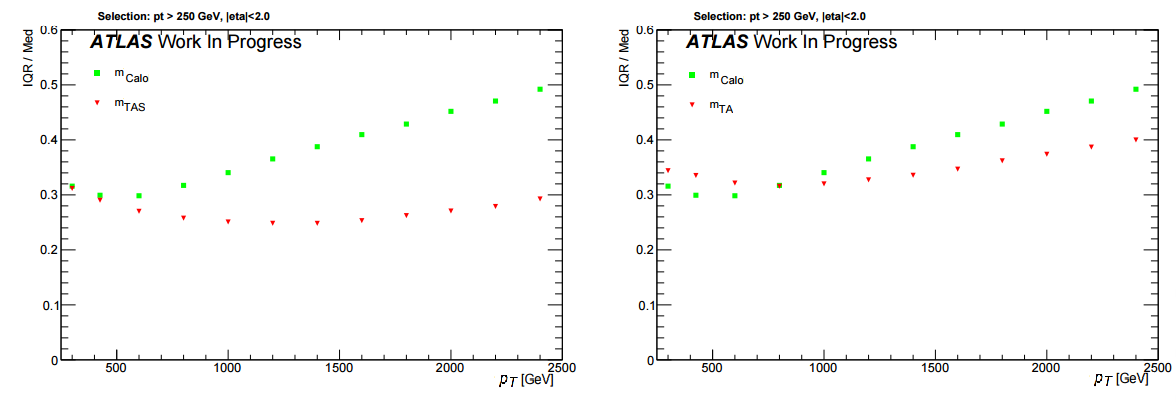
\includegraphics[width=\textwidth]{jet_part/mtas/qcdmtas.png}
        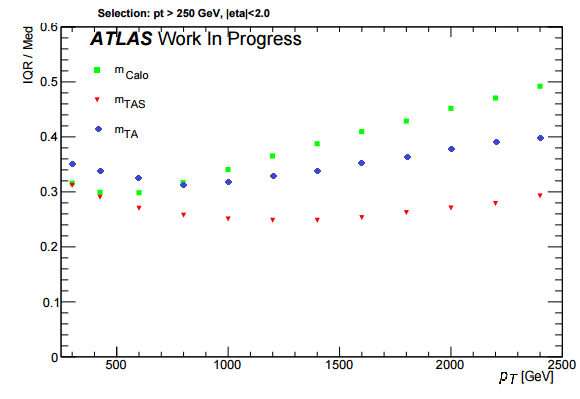
\includegraphics[width=0.7\textwidth]{jet_part/mtas/qcdmtastruffa.png}
   \caption[$\mtas$ for QCD jets]{Performance of the $\mtas$ versus the $\mcal$ and $\mta$ for the QCD multijet. Here shown IQR/Med not $\iqr$.}
  \label{fig:mtas5}
\end{figure}

\subsection{Performance in Massive $\tilde{W}\to q'\bar{q}$ Decays with $m_{\tilde{W}}=m_t$}
The massive $W$ sample is a special sample which was used to understand the behavior of the boosted tops, whether its worse resolution was coming from the higher mass of the top quark or from the more complex decay topology (three-pronged instead of two-pronged decay and b-quark presence). 
The sample is almost identical to the boosted $W/Z$ one ($W'\to WZ$) but in this case the SM electroweak boson are set to have the mass of the top quark $m_{\tilde{W}}=m_t$.
In fact, from the rule $\Delta R=2m/p_T$, a bigger separation is expected between the quark from the hadronic decay.
The comparison with $\mcal$ is shown in Figure \ref{fig:mtas6}, together with the boosted top-quark for comparison. As seen here, the performance of the latter is clearly worse than the former, the trend is yet very similar. This difference is interpreted in terms of different and more complex topology and hence higher sub-jet multiplicity: in the three sub-jet structure, resolving accurately the components is more challenging.

\begin{figure}[!ht]
  \centering
     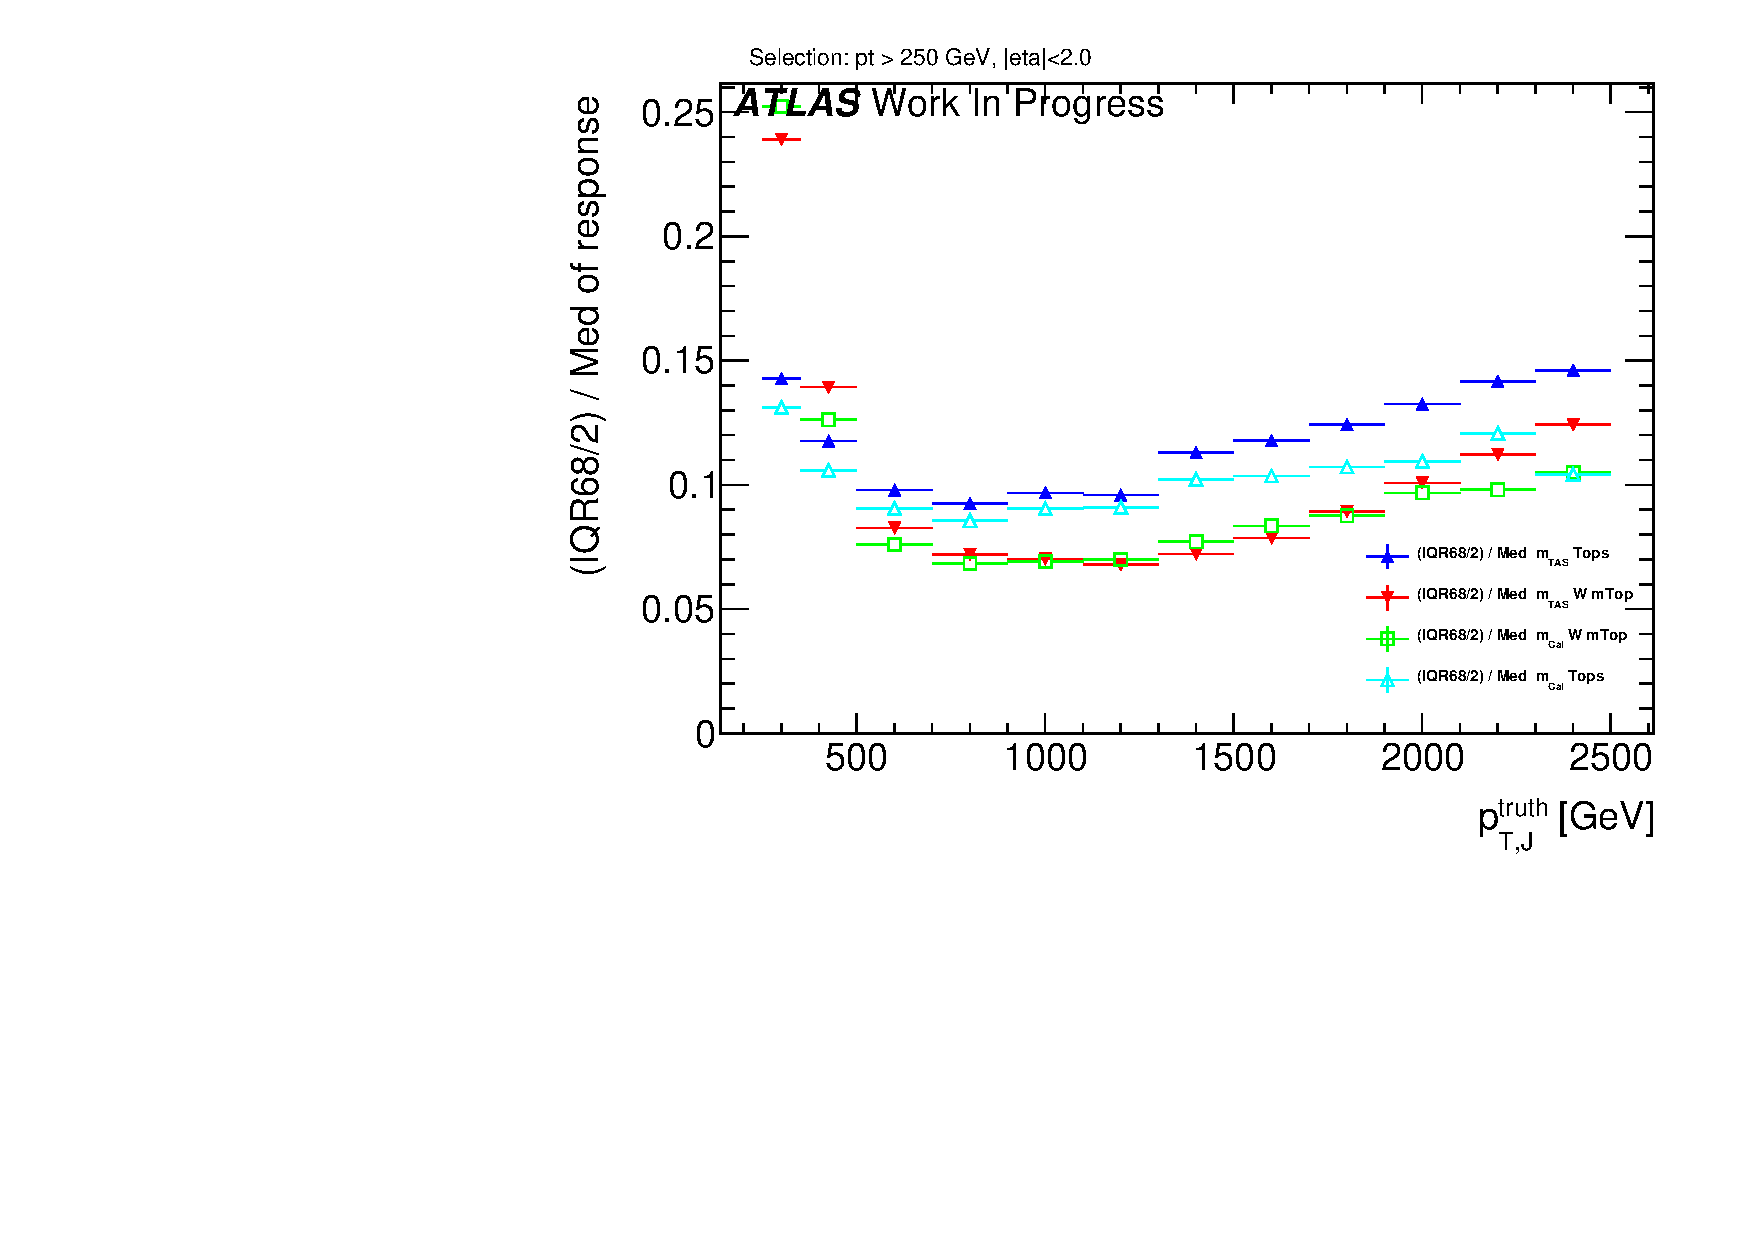
\includegraphics[width=0.7\textwidth]{jet_part/mtas/71graphcftr_h_JetRatio_mJ12CALOIQRoMcalib_WmassiveVsTops.pdf}
   \caption[$\mtas$ for boosted massive $W/Z$]{Performance of the $\mtas$ versus the $\mcal$ for the massive $W/Z$ (in red and green); shown on the same plot also the boosted top sample (in blue and light blue).}
  \label{fig:mtas6}
\end{figure}

\subsection{Other Stability Quantifiers}
The stability of the $\mtas$ was checked, although the IQnR is already a good quantifier of stability, explicitly for the mean of the mass response distribution and for the left-hand-side tail, as a function of the transverse momentum. This was an important check to assure the overall gaussianity of the final distribution in the whole spectrum of $\pt$, and suitability in regards of the calibration step, which is not discussed in this thesis.

The mean of the response distribution is shown for boosted $W/Z$ decays in Figure \ref{fig:meanandtail}, left; as seen here, despite being the mean constantly below the unity, its behavior is much more flat and independent of $\pt$, especially in the low-middle regime. This is surprising since the $\mcal$ is already shown after the calibration step, which is not taken instead for the $\mtas$. Conversely the left-hand-side tail of the mass response which is shown in the same figure, right, shows a more enhanced behavior than the $\mcal$, but still never reaches the 10\%. Of course an enhancement of the tail causes a loss of gaussianity and a number of jets which are reconstructed with a lower mass than they should, but it is still comparable with the calorimeter mass.

Those quantifiers show analogous behavior for the other samples considered and those figures can be found in the Appendix.

\begin{figure}
    \centering
    \begin{subfigure}[b]{0.45\textwidth}
	\centering
        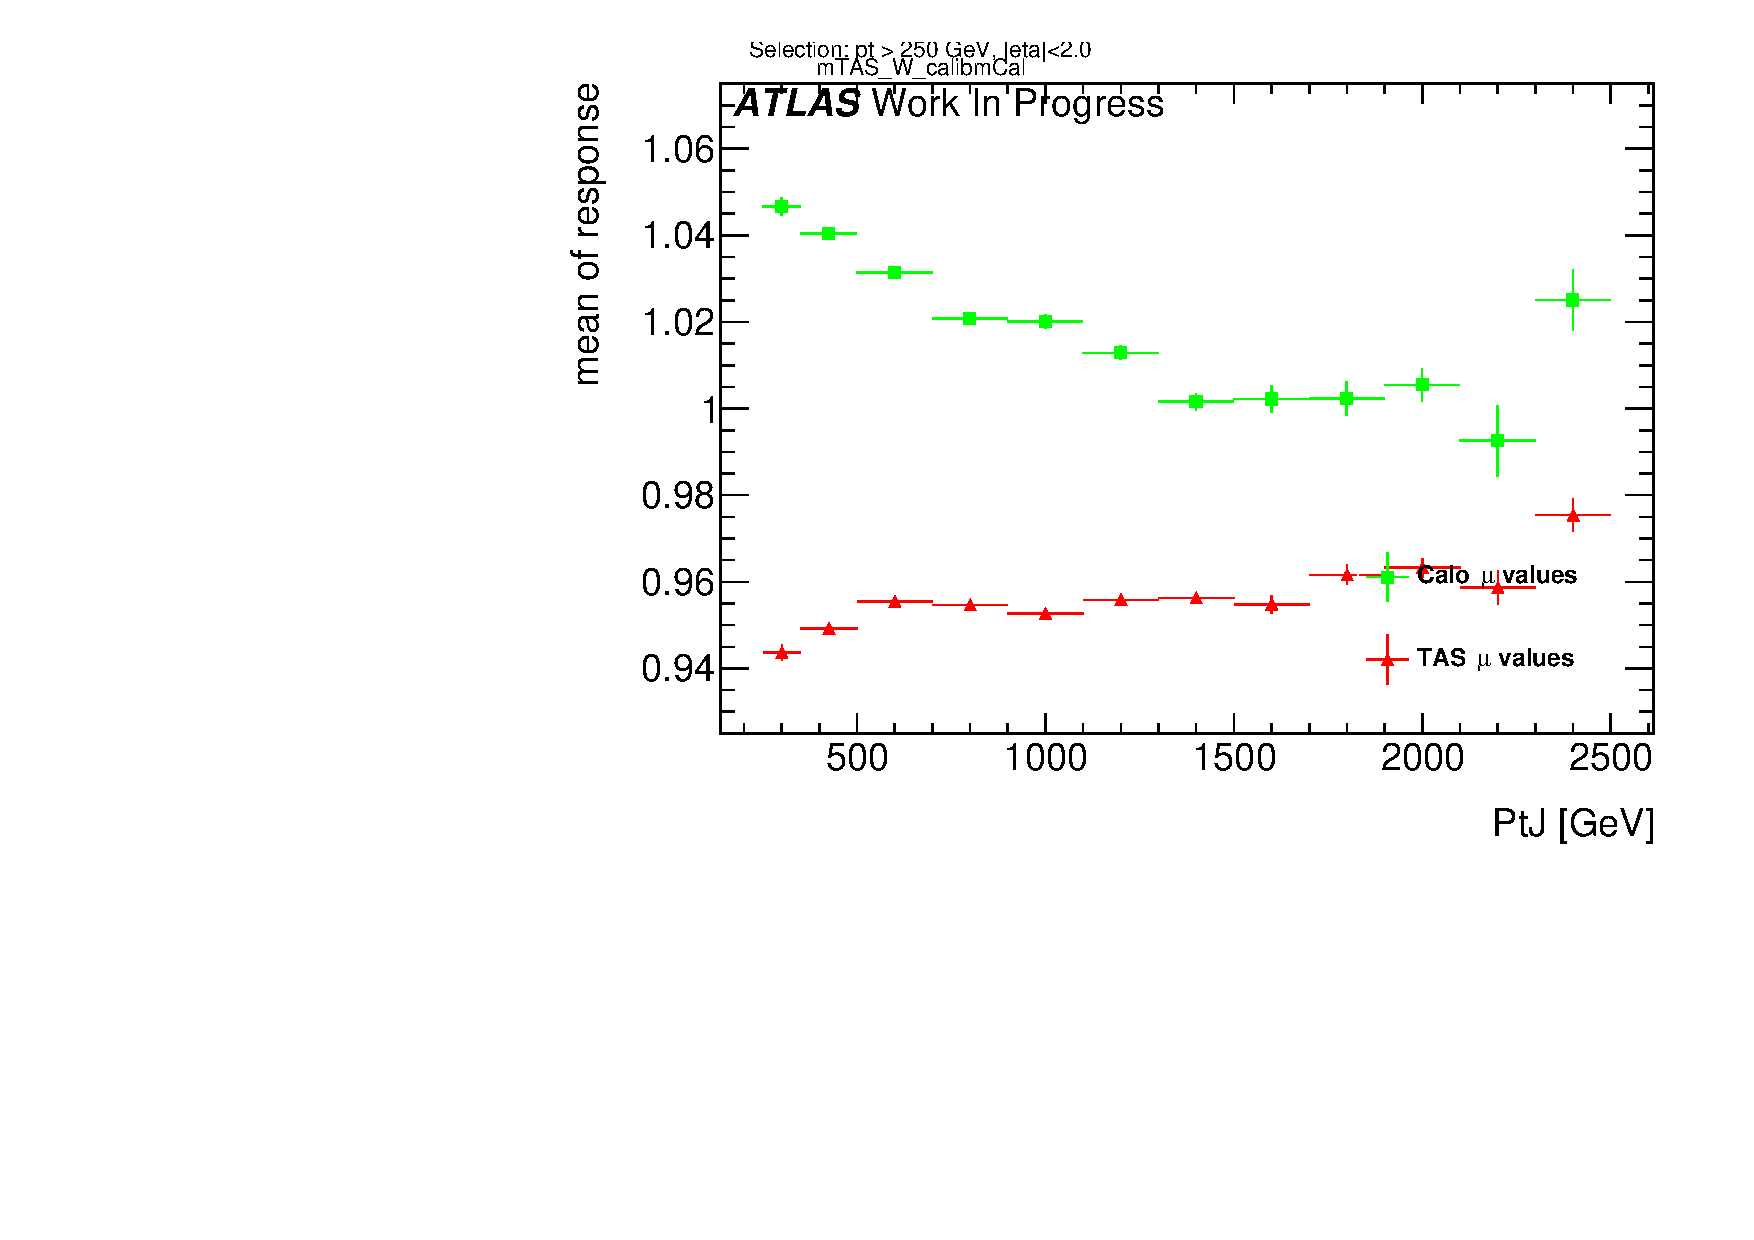
\includegraphics[width=\textwidth]{appendixB/mTAS_W_calibmCal_20:07:01-03-11-2016/71graph_h_JetRatio_mJ12CALO_meanResponseMvsTA.pdf}
%         \label{fig:tiger}
    \end{subfigure}
    \begin{subfigure}[b]{0.45\textwidth}
	\centering
        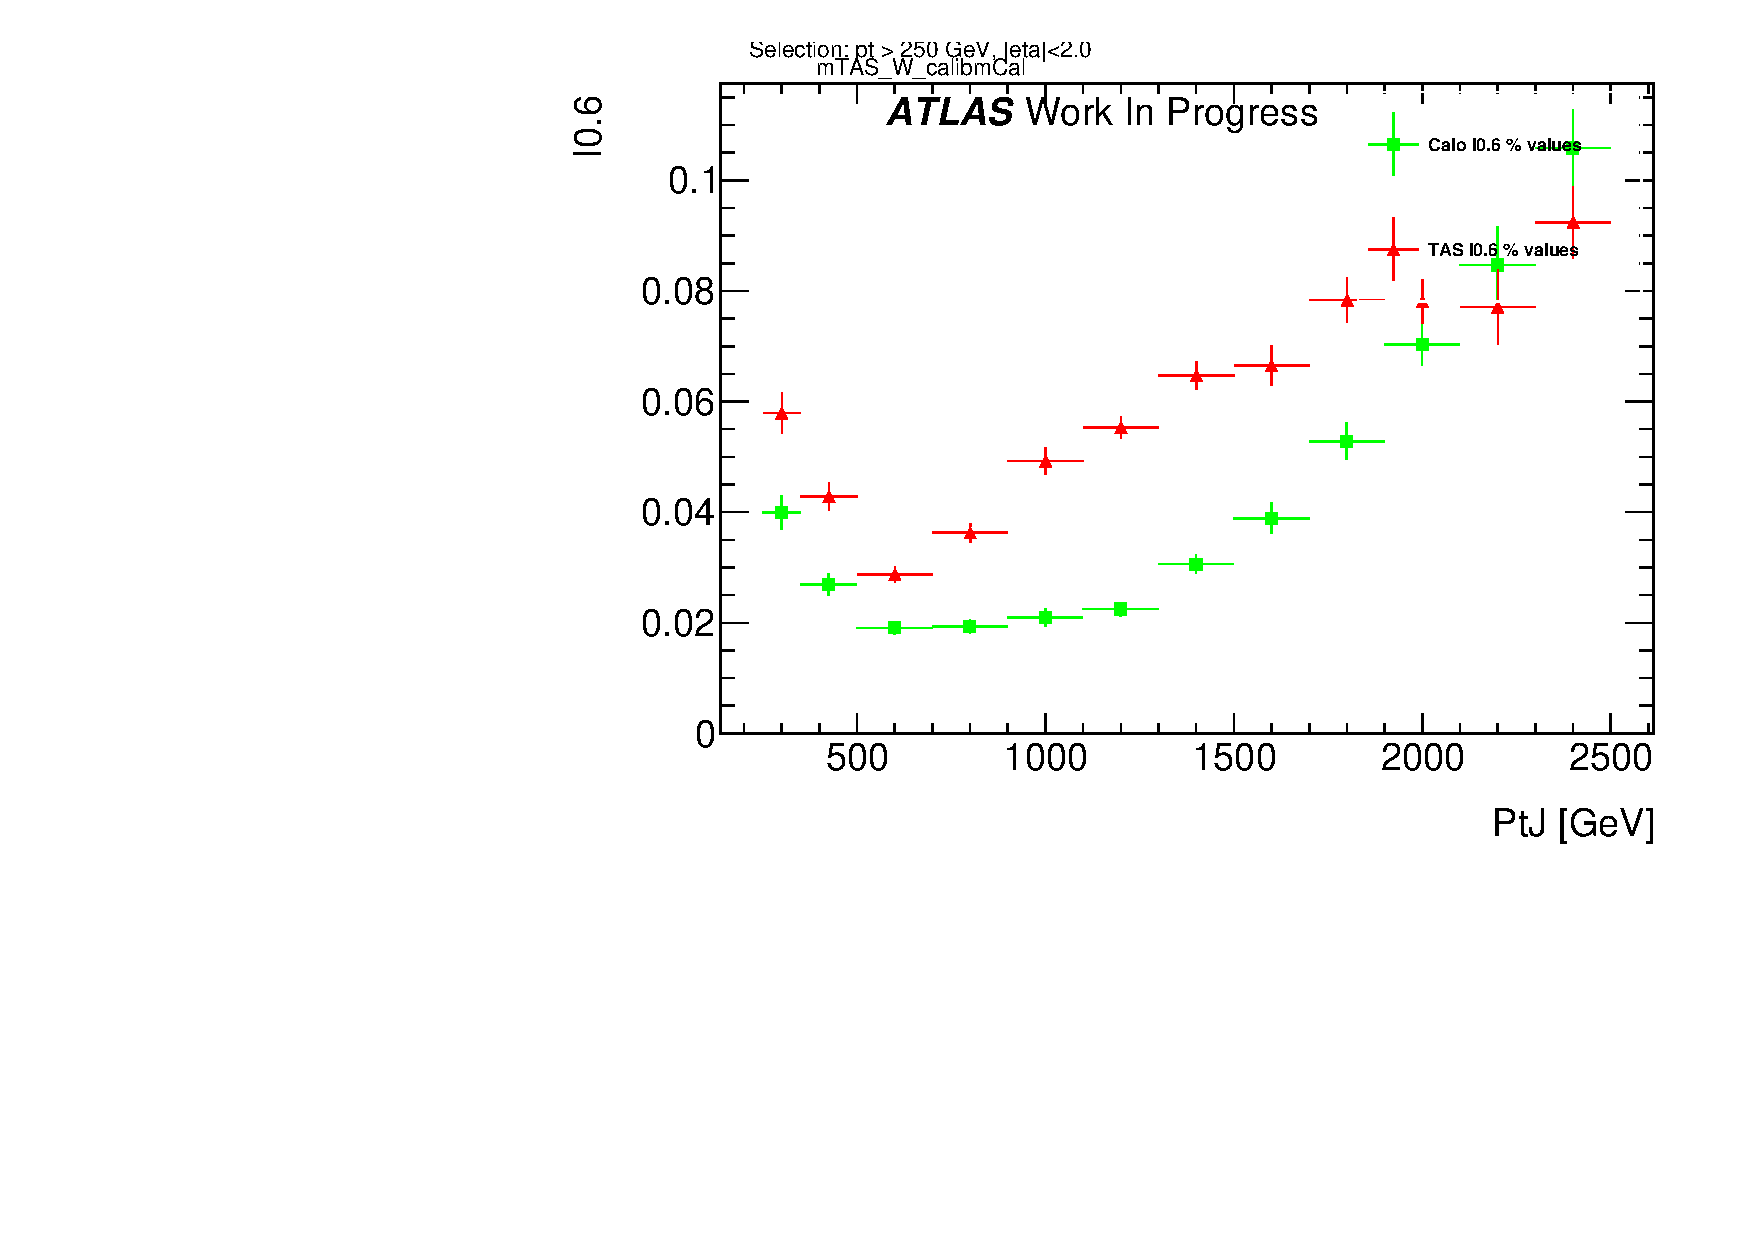
\includegraphics[width=\textwidth]{appendixB/mTAS_W_calibmCal_20:07:01-03-11-2016/74graph_h_JetRatio_mJ12CALO_I50ResponseMvsTAnorm.pdf}
 
%         \label{fig:gull}
    \end{subfigure}
    \caption[Mean and left-hand side integral for boosted $W/Z$]{Stability quantifiers which were checked for the $\mtas$: mean, on the left, and normalized left-hand side integral, on the right, of the mass response distribution. The mean is calculated from a Gaussian fit and the integral goes from 0 to 0.6.} 
    \label{fig:meanandtail}
\end{figure}

\subsection{Sub-jet Calibration}

An additional attempt of calibrating the sub-jet was also tried and, although the results were not substantially improved, it is presented in this section. This study was performed using only boosted $W/Z$ samples.

\subsection{Preliminary Studies on Sub-jet Calibration}
The first attempt in calibrating the sub-jets had as start a ``perfect calibration'', which means using the truth-level information from the MC sample \textit{before} the interaction with the calorimeter.
Truth-level tracks are the particles in the jet which have an electric charge and are stable, truth-level sub-jets are all the particles, charged and not, which are ghost associated to the calorimeter sub-jets.
There are few possibilities in doing so, here some nomenclature for this study will be introduced:
\begin{itemize}
 \item $\mtas$ using truth-level sub-jets and tracks; normal tracks (with all detector effects) are used to assist the truth-level sub-jets;
 \item $\mtas$ using truth-level tracks and truth-level sub-jets; the truth-level tracks are used to assist the truth-level sub-jets;
 \item $\mcal$ truth, calculated using only the truth sub-jets.
\end{itemize}


\subsubsection{Perfect Calibration}
The \textit{perfect calibration} refers to the procedure of using $\mtas$ with truth-level sub-jets and track, i.e. looking at the best possible scenario with an ideal detector. The performance is of course expected to be optimal, because of the use of the truth-level. This step was necessary as feasibility study, to understand whether ulterior efforts in this direction were meaningful.
The perfect calibration is shown in Figure \ref{fig:perfcalib}; since the performance exhibits room for big improvement below $\sim$ 1 TeV and moderate to small improvement above this value, the second step of a simple calibration was tried.

\begin{figure}[!ht]
  \centering
      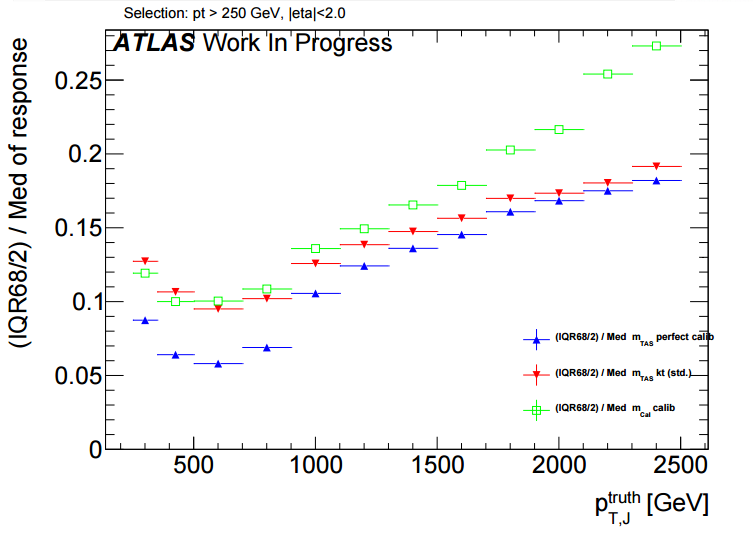
\includegraphics[width=0.7\textwidth]{jet_part/calib/perfcalib.png}
  \caption[Perfect calibration]{Performance of the perfect calibration. It shows room for improvement especially at low-middle $\pt$.}
  \label{fig:perfcalib}
\end{figure}


\subsubsection{Simple Sub-jet Calibration}
Following the example of calibration of jets in general, a simple approach to emulate this procedure was tried, constructing in various bins of transverse momenta the responses of the sub-jet's energy to derive the weights factors to be applied. The detailed procedure is as follows:
\begin{enumerate}
 \item Responses in energy $R_E=E^{reco}/E^{truth}$ were built in several bins of $\pt$, spanning to the whole transverse momentum range;
 \item The mean $\mu_R$ of this response was calculated via a fit to the Gaussian core;
 \item Those values (\textit{scale factors}) were stored and applied again to the sub-jets before the computation of the $\mtas$ via 4-momentum correction $E'=E/\mu_R$; the $\pt$ (the value which only enters the $\mtas$ variable) was changed then correspondingly to keep the sub-jet's mass constant.
\end{enumerate}

This procedure was called \textit{poor man's calibration} or PM calibration or \textit{simple calibration}.
A check on the $\pt$ response before and after calibration together with the mean of the entire Large-$R$ jet response is shown in Figure \ref{fig:calibA} and \ref{fig:calibA2} in Appendix.

The results are on Figure \ref{fig:perfcalib4}; there are only marginal improvements in few ranges of low transverse momentum where the scale factors are further away from unity, and the overall observable is not performing better than the standard $\mtas$. This is interpreted both in terms of a missing calibration as a function of the $\eta$ variables (having hence a befit from the crack region) and because the correction done on average does not provide the sufficient handle in a jet-by-jet basis, especially when all the sub-jets are rescaled by similar factors (which translates into a similarity of $\pt$s of the sub-jets, often the case for e.g. boosted $W/Z$, less for boosted tops entirely contained in the large-$R$ jet).

\begin{figure}[!ht]
  \centering
      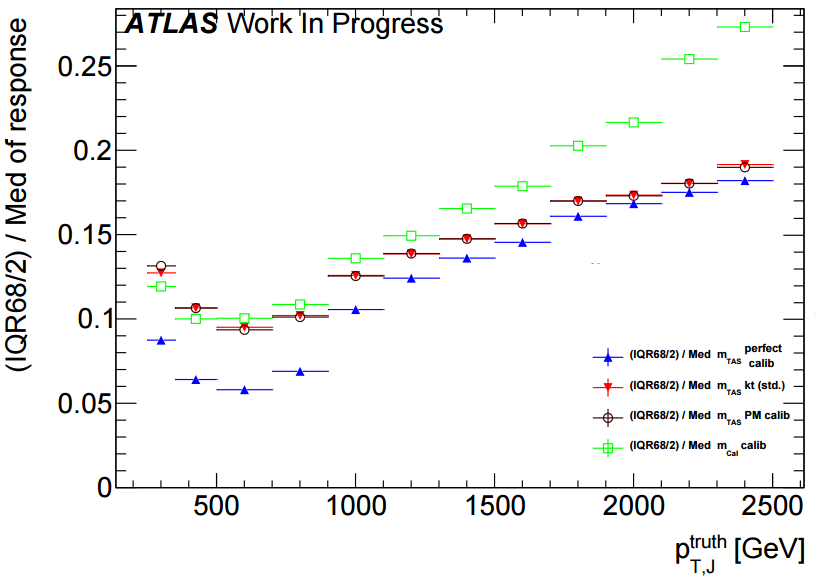
\includegraphics[width=0.7\textwidth]{jet_part/calib/perfectcalib4.png}
  \caption[Simple calibration]{Performance of the poor man's calibration. The improvement is marginal throughout the entire transverse momentum space.}
  \label{fig:perfcalib4}
\end{figure}

\subsection{Limitation of $\mtas$}
The final effort to understand the various and competing effects, which take place in the $\mtas$ and which was inspired by the perfect calibration procedure, brought to a final study on the variable to understand the reason for the worsening of the resolution at high transverse momenta, using again the truth MC information.

The preliminary investigation in this direction was then the study on the track-resolution: since the track relative resolution of the transverse momentum is expected to worsen linearly with this variable, a response of the mass of the tracks was constructed, using the truth-level tracks.

The result is shown on Figure \ref{fig:trackdegrade}: for the samples considered, it shows a linear degradation of the mass of the tracks, both for massive and SM $W/Z$.

\begin{figure}[!ht]
  \centering
      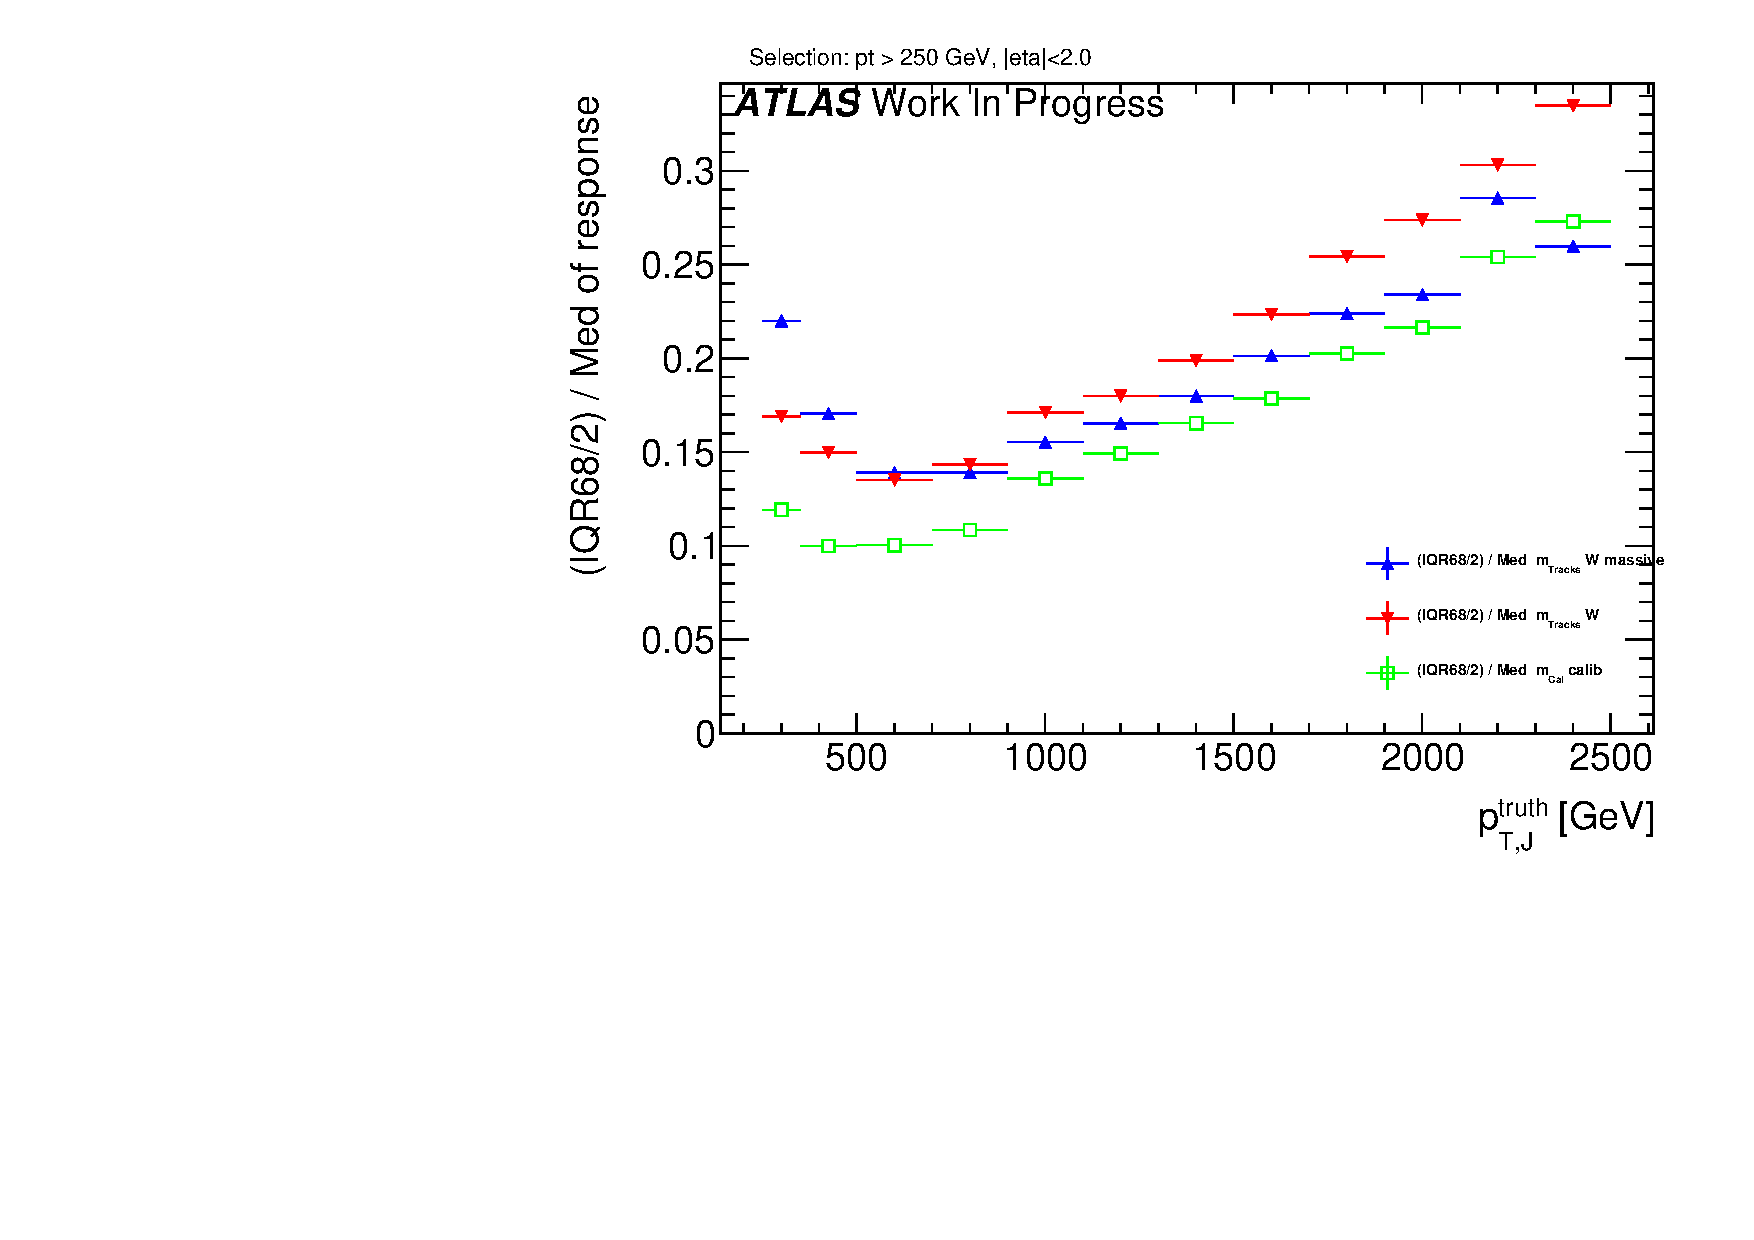
\includegraphics[width=0.7\textwidth]{jet_part/calib/71graphcftr_h_JetRatio_mJ12CALOIQRoMcalib_trkmass.pdf}
  \caption[Track mass degradation in tops and massive $W/Z$]{The performance of the track mass in blue and red for massive $W$ sample and boosted $W/Z$ respectively; for reference in green the calorimeter mass of the large-$R$ jet.}
  \label{fig:trackdegrade}
\end{figure}

The hypothesis of the degradation of the $\mtas$ driven by the tracks is also supported by the Figure \ref{fig:breakdown1} in Appendix, where the truth-level tracks are used instead of real tracks to compute the variable; it can be seen the flat behavior at high $\pt$, hence ascribing the worsening of the resolution to tracks at higher transverse momenta.


A complete breakdown of the variable in terms of truth-level particles is given in Figure \ref{fig:breakdown2}, where all the different components are separated.
In particular the black dots show the $\mtas$ using truth-level sub-jets but real tracks for the track assistance procedure.
Even combining this truth-level information, in fact, it shows a large worsening of the performance (truth-level sub-jets only are shown as blue dots).

% Particularly interesting is the black dots, which 
% uses truth-level sub-jet but real tracks, which worsen the overall performance of the truth-level sub-jet alone (shown in light blue dots).

\begin{figure}[!ht]
  \centering
      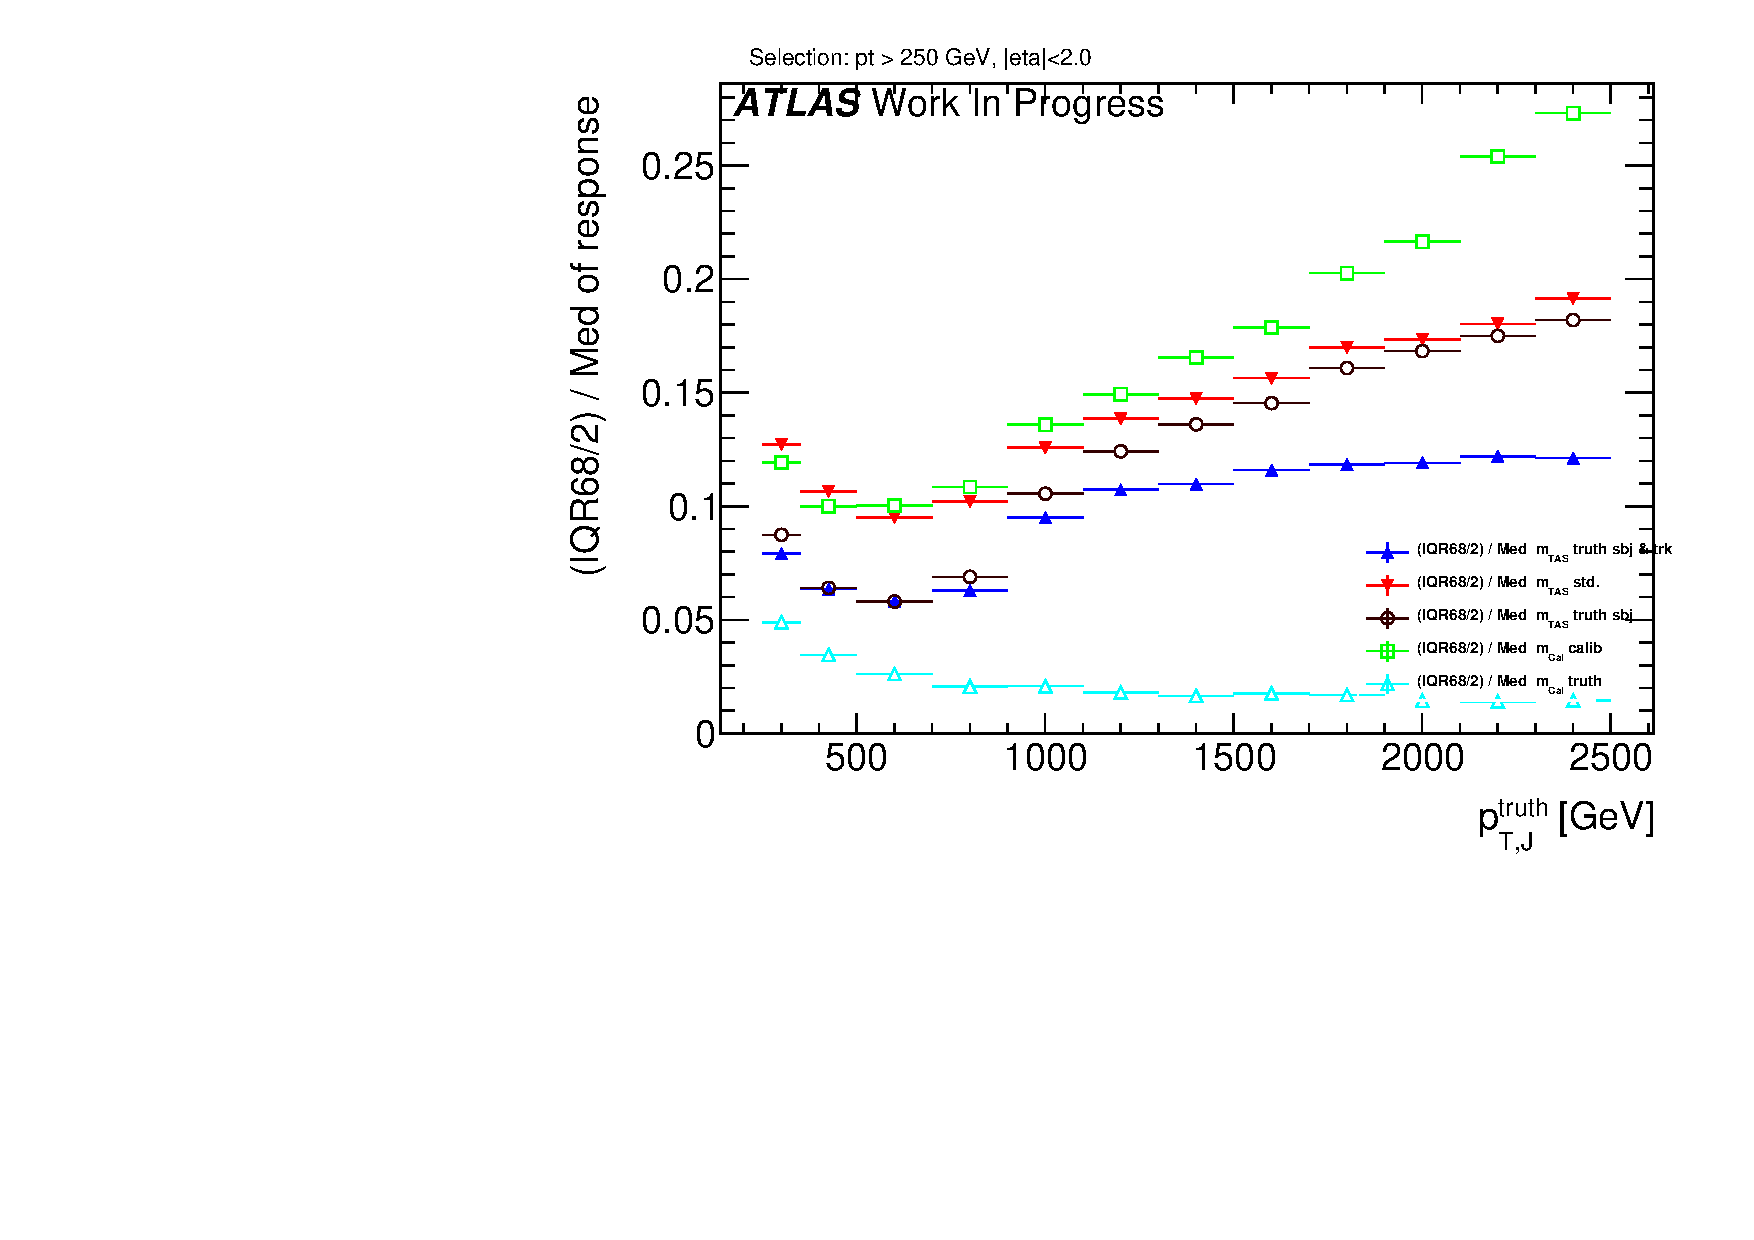
\includegraphics[width=0.7\textwidth]{jet_part/calib/71graphcftr_h_JetRatio_mJ12CALOIQRoM4Truths.pdf}
  \caption[Breakdown of the $\mtas$ ]{Breakdown of the $\mtas$ in its component using truth-level information for boosted $W/Z$ decays.}
  \label{fig:breakdown2}
\end{figure}

Other results using truth-level information on boosted tops are shown and described in the Appendix.


% \subsection{Large-R jet: Calibration}
% The jet mass scale calibration aims to correct the reconstructed jet mass to the particle-level jet mass by applying calibration factors derived from a sample of simulated QCD multijet events, with an analogous procedure described in \ref{sec:calib} for the jet energy scale.
% 
% \subsection{Large-R jet: Uncertainties}


\subsection{Alternative Observable Definitions}
\label{sec:alternate}

There are quite a few ways to modify the track-assisted sub-jet mass; however, all the alternative approaches showed worse performance, and they are mentioned here for completeness only.

Alternatives considered were: 
\begin{itemize}
 \item for the tracks:
 \begin{itemize}
   \item use of tracks not as input directly, but only taking those belonging to anti-k$_t$ reclustered track-jet with radius of 0.3 or 0.2;
   \item tighter or looser quality conditions were explored;
   \item tighter or looser primary vertex association requirement were explored.
 \end{itemize}
 \item for the sub-jets:
  \begin{itemize}
   \item the trimming procedure was modified: various radii $R_{sub}$ of the sub-jets were tested;
   \item the sub-jets were reclustered using not only the standard k$_t$, but also anti-k$_t$ and C/A.
  \end{itemize}
  \item for the procedure: different 4-momentum correction scheme was also explored.
\end{itemize}

The different reclustering algorithm choice has a deep impact and was studied in details, since it changes the topo-cluster added to the sub-jets and the tracks associated to them. The situation is depicted in the event-display in Figure \ref{fig:evtdspl}; the display on the left shows the standard choice of k$_t$, the one on the right shows the modified approach anti-k$_t$. 

In the Appendix, figure \ref{fig:allalgow} \ref{fig:allalgotop} \ref{fig:allalgohiggs} the performance for boosted $W/Z$, tops and Higgs are shown, respectively. It can be seen that the k$_t$ algorithm provides the best observable definition, in all the samples considered. However, the anti-k$_t$ algorithm provides similar performances; this was an important check as the jet calibration procedure currently going on in ATLAS, the \textit{R-Scan} procedures includes the anti-k$_t$ algorithm with radius of R=0.2 and aims at providing the calibration and uncertainties that could be used directly in the computation of the $\mtas$.

\begin{figure}[!ht]
  \centering
      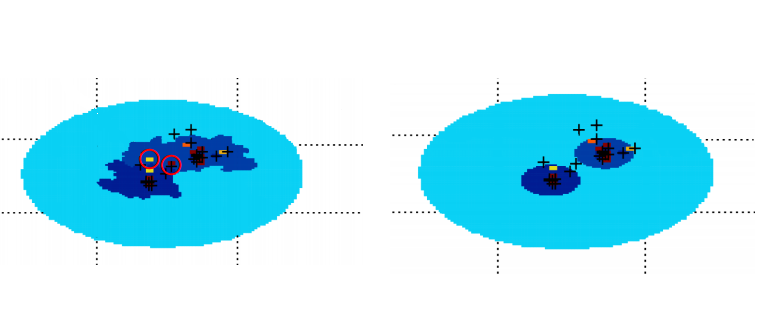
\includegraphics[width=0.7\textwidth]{jet_part/mtas/evtdspl.png}
  \caption[Different reclustering in event display]{An example of event-display shows the differences in the reclustering algorithm used for the sub-jets: on the right  k$_t$ and on the left anti-k$_t$. Highlighted some constituents trimmed away with the second choice.}
  \label{fig:evtdspl}
\end{figure}

\section{Combining the mass observables}


Since the calorimeter large-$R$ jet mass is not explicitly used in the track-assisted (sub-jet) mass, it may be possible to improve the performance creating a new observable which combines both mass definitions.


\begin{figure}[!ht]
  \centering
      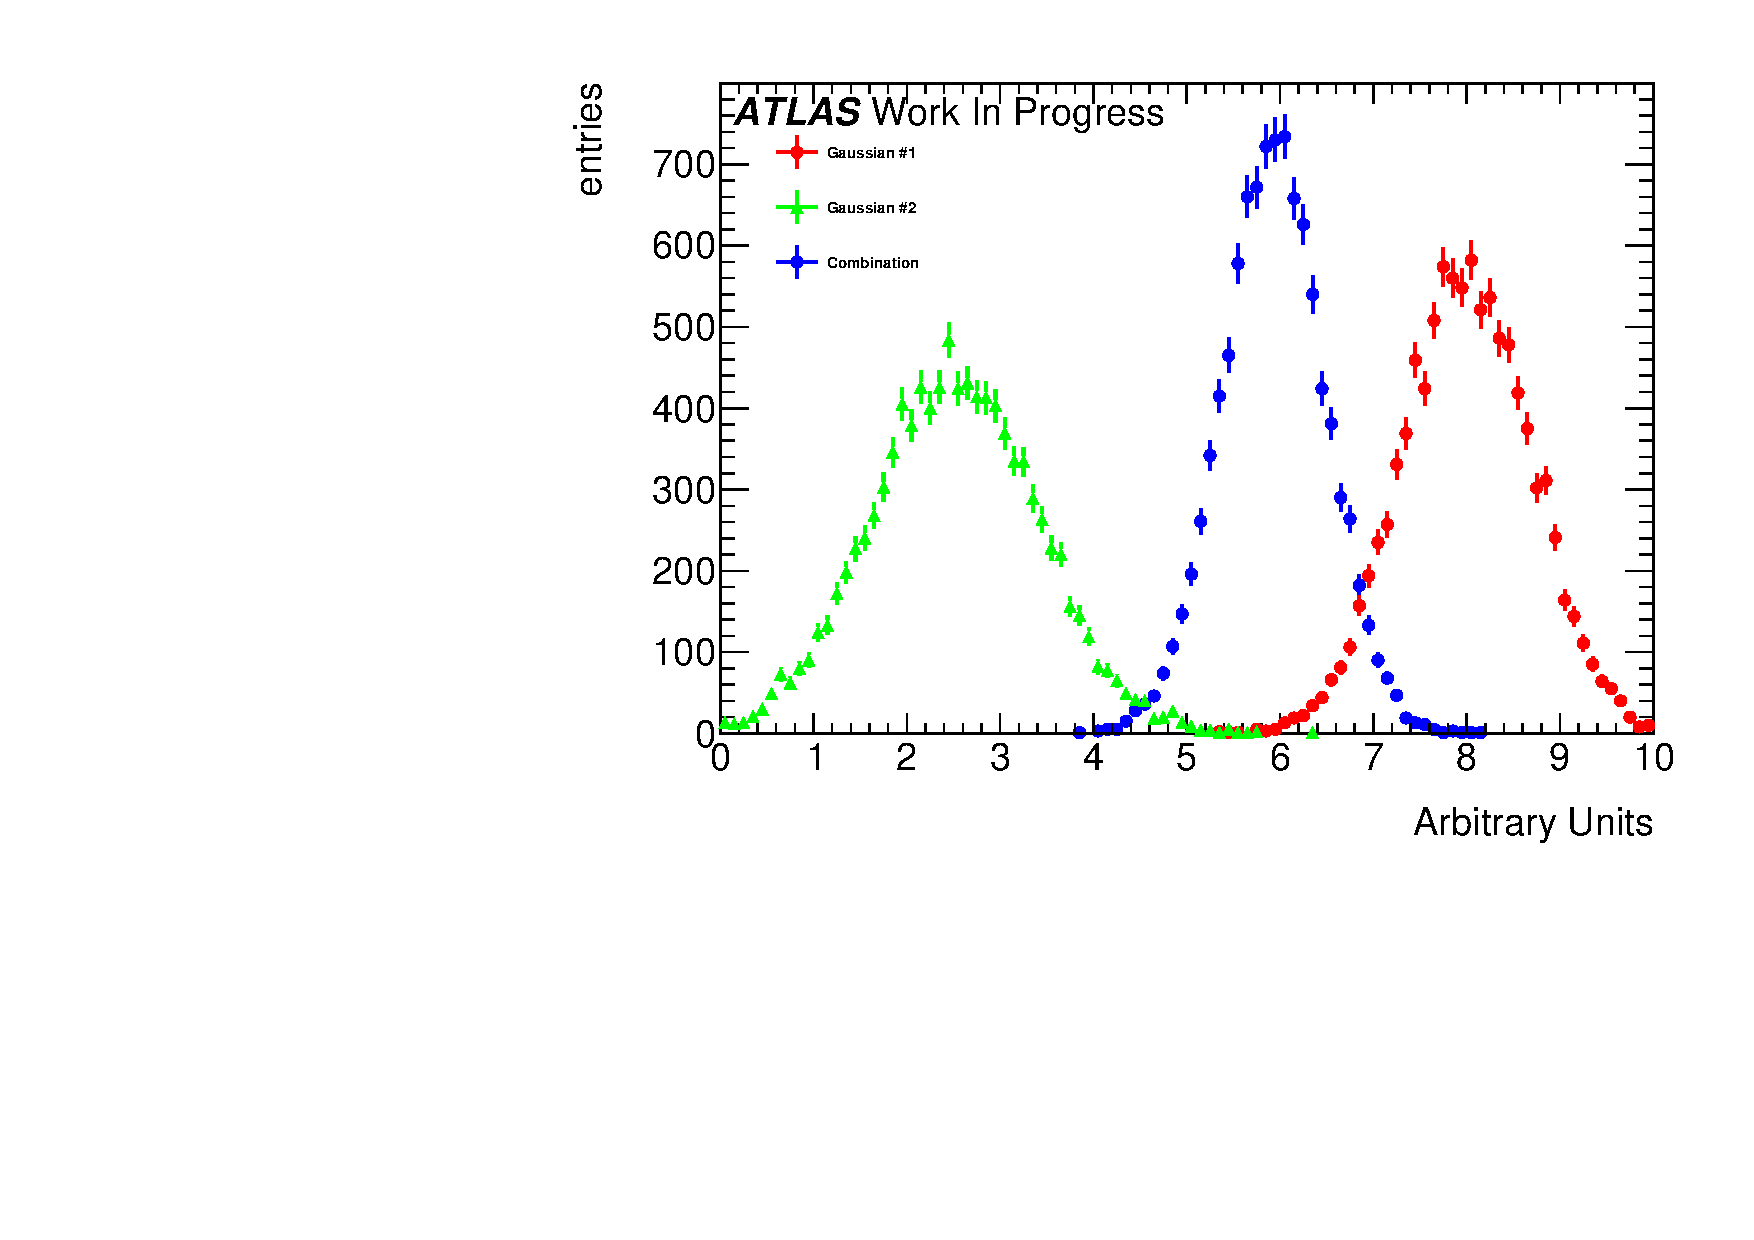
\includegraphics[width=0.7\textwidth]{jet_part/mcomb/example.pdf}
  \caption[Toy example of Gaussian combination]{A toy example of the combination of two independent Gaussian observables, in red and green, and their combination, in blue. It can be seen that the combination has a smaller width.}
  \label{fig:mcomb1}
\end{figure}

This is true for both the $\mta$ and the $\mtas$; they are introduced in the next subsections.
Provided that the two observables are nearly independent (correlation coefficient are $\sim$ 10\%, see Figure \ref{fig:mcomba1} in the Appendix), due to the Gaussian nature of the $\pt$ and mass response, the optimal combination of the two is linear\footnote{If the joint distribution of the responses is Gaussian, then one can write their probability distribution function as $f(x,y)=h(x,y)\times \exp[A(\mu)+T(x,y)\mu]$, where $x$ is the calorimeter-based jet mass response, $y$ is the track-assisted jet mass response,
$\mu$ is the common average response, and $h$, $A$,$T$ are real-valued functions. This form shows that the distribution is from the exponential family and therefore $T$ is a sufficient statistic. Since the natural parameter space is one-dimensional, $T$ is also complete. Therefore, the unique minimal variance unbiased estimator of $\mu$ is the unique unbiased function of $T(x, y) =x/\sigma^2_x \times + y/\sigma^2_y$.
See e.g. Ref. \cite{statistic} and \cite{art35} for details.}.
An example is provided in Figure \ref{fig:mcomb1}.
\subsection{Combination $\mta-\mcal$ }

For the $\mta-\mcal$ combination the observable are considered nearly independent, then
\begin{equation}\begin{split}
 \mcomb= a\times \mcal + b \times \mta,\\
 a=\frac{\sigma_{calo}^{-2}}{\sigma_{calo}^{-2}+\sigma_{TA}^{-2}} \qquad b=\frac{\sigma_{TA}^{-2}}{\sigma_{calo}^{-2}+\sigma_{TA}^{-2}}
\end{split}
\label{eq:mtacomb}
\end{equation}
where $\sigma_{calo}$ and $\sigma_{TA}$ are the $\mcal$'s and $\mta$'s resolution functions. The $\mcomb$ then is the $\mta-\mcal$ combination.

\subsection{Combination $\mtas-\mcal$ }

There is a main difference between the $\mtas$ and $\mta$ when it comes to combination: since the $\mtas$ is using sub-jet level information but $\mta$ not, the correlation with the $\mcal$ is expected to be higher.
This can be seen e.g. in the plots in Figure \ref{fig:mcomb2} (additional plots shown in Figure \ref{fig:mcomba2} in Appendix), where the correlation is not only higher for the simple $W/Z$ and Higgs jets, but above 50\% for tops. The assumption of independent variables here falls, forcing a more complete approach. The Ansatz is to take into account the correlation via the formula:
\begin{equation}
\begin{gathered}
\mcombtas= w\times\mcal + (1-w)\times\mtas,\\
w=\frac{\sigma_{TAS}^2-\rho\sigma_{calo}\sigma_{TAS}}{\sigma_{calo}^2+\sigma_{TAS}^2-2\rho\sigma_{calo}\sigma_{TAS}}
\end{gathered}
\label{eq:mtascomb}
\end{equation}
% 
where now $\mcombtas$ is the new $\mtas-\mta$ combination. This expression reduces then to the form:
\begin{equation}
\begin{gathered}
\mcombtas= a\times\mcal + b\times\mtas,\\
a=\frac{\sigma_{TAS}^2-\rho\sigma_{calo}\sigma_{TAS}}{\sigma_{calo}^2+\sigma_{TAS}^2-2\rho\sigma_{TAS}\sigma_{calo}}\qquad b=\frac{\sigma_{calo}^2-\rho\sigma_{calo}\sigma_{TAS}}{\sigma_{calo}^2+\sigma_{TAS}^2-2\rho\sigma_{TAS}\sigma_{calo}}
\end{gathered}
\end{equation}
which reduces to equation \eqref{eq:mtacomb} after simple algebra for the case when $\rho=0$. Of course, this value can be set to the value of the specific sample considered, or to an average of 0.3 if one wants to give a definition generally valid for all the cases considered; in this case, the performance would be slightly sub-optimal.

\subsubsection{Procedure}
The procedure of producing the $\mcombtas$ is defined as follows:
\begin{enumerate}
 \item For the given sample, the $\mtas$ and $\mcal$ are produced;
 \item The mass responses are also produced for the given ranges of $\pt$;
 \item For each of these responses, the value of the IQnR as defined previously is calculated and stored;
 \item The average correlation factor of 0.3 is assumed;
 \item With the formula \ref{eq:mtascomb}, $\mcombtas$ is calculated using the $\mtas$, $\mcal$ and the values stored from before.
\end{enumerate}
A remark on the procedure: the step 3. uses values of the IQnR because this was showed to be a more robust way to look at the response and fit-independent. For step 4. the correlation factor was decided to be and average of the samples considered.

Additionally, the IQnR weights are produced for each sample specifically. In order to give a sample-independent definition of the $\mcombtas$, following also the procedure adopted for the $\mcomb$, these weights could be taken from a QCD multijet sample and applied indiscriminately to the particular case. Here of course the performance would be again sub-optimal, since the variable was not developed in an ad-hoc way.

Throughout the results presented in the following sections, both observables were calculated with ad-hoc weights. Quantitative statements between them would still hold in the case of QCD weights. However, when confronting e.g. $\mtas$ with them it has to be kept in mind that in this case their performance is overestimated, since this choice, although being more general, would perform slightly worse.

\begin{figure}[!ht]
  \centering
      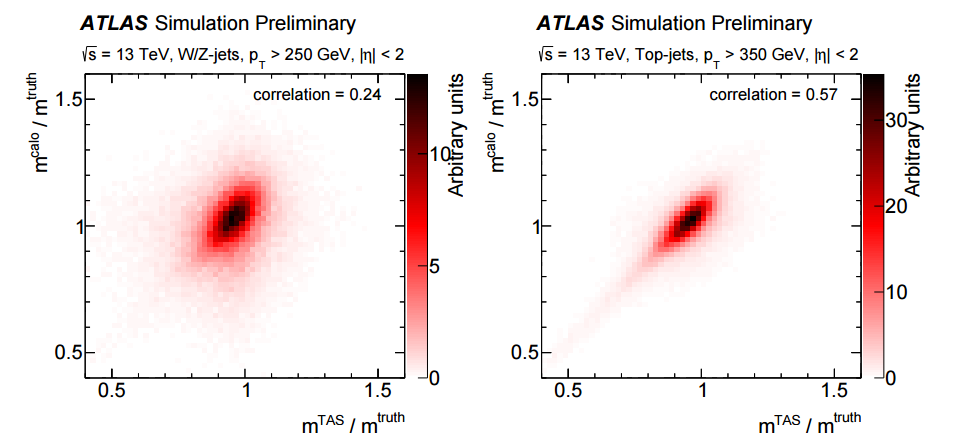
\includegraphics[width=0.7\textwidth]{jet_part/mcomb/mcomb2.png}
  \caption[$\mcal$ and $\mtas$ correlation plots]{The calorimeter based jet mass mass response versus the track-assisted sub-jet mass response, on the left for boosted $W/Z$ on the right for boosted tops.}
  \label{fig:mcomb2}
\end{figure}

\subsection{Performance in $W \to q'\bar{q}$ Decays}
On the boosted $W/Z$s sample, the performance of the $\mcombtas$ outperforms all the other definitions throughout all the transverse momentum space; on Figure \ref{fig:mcombtas3} they are shown for reference together with the $\mtas$. It can be noted here that the track-assisted sub-jet mass, although being sub-optimal, has comparable performance, yet presenting fewer complications due to the combination procedure.

\begin{figure}[!ht]
  \centering
      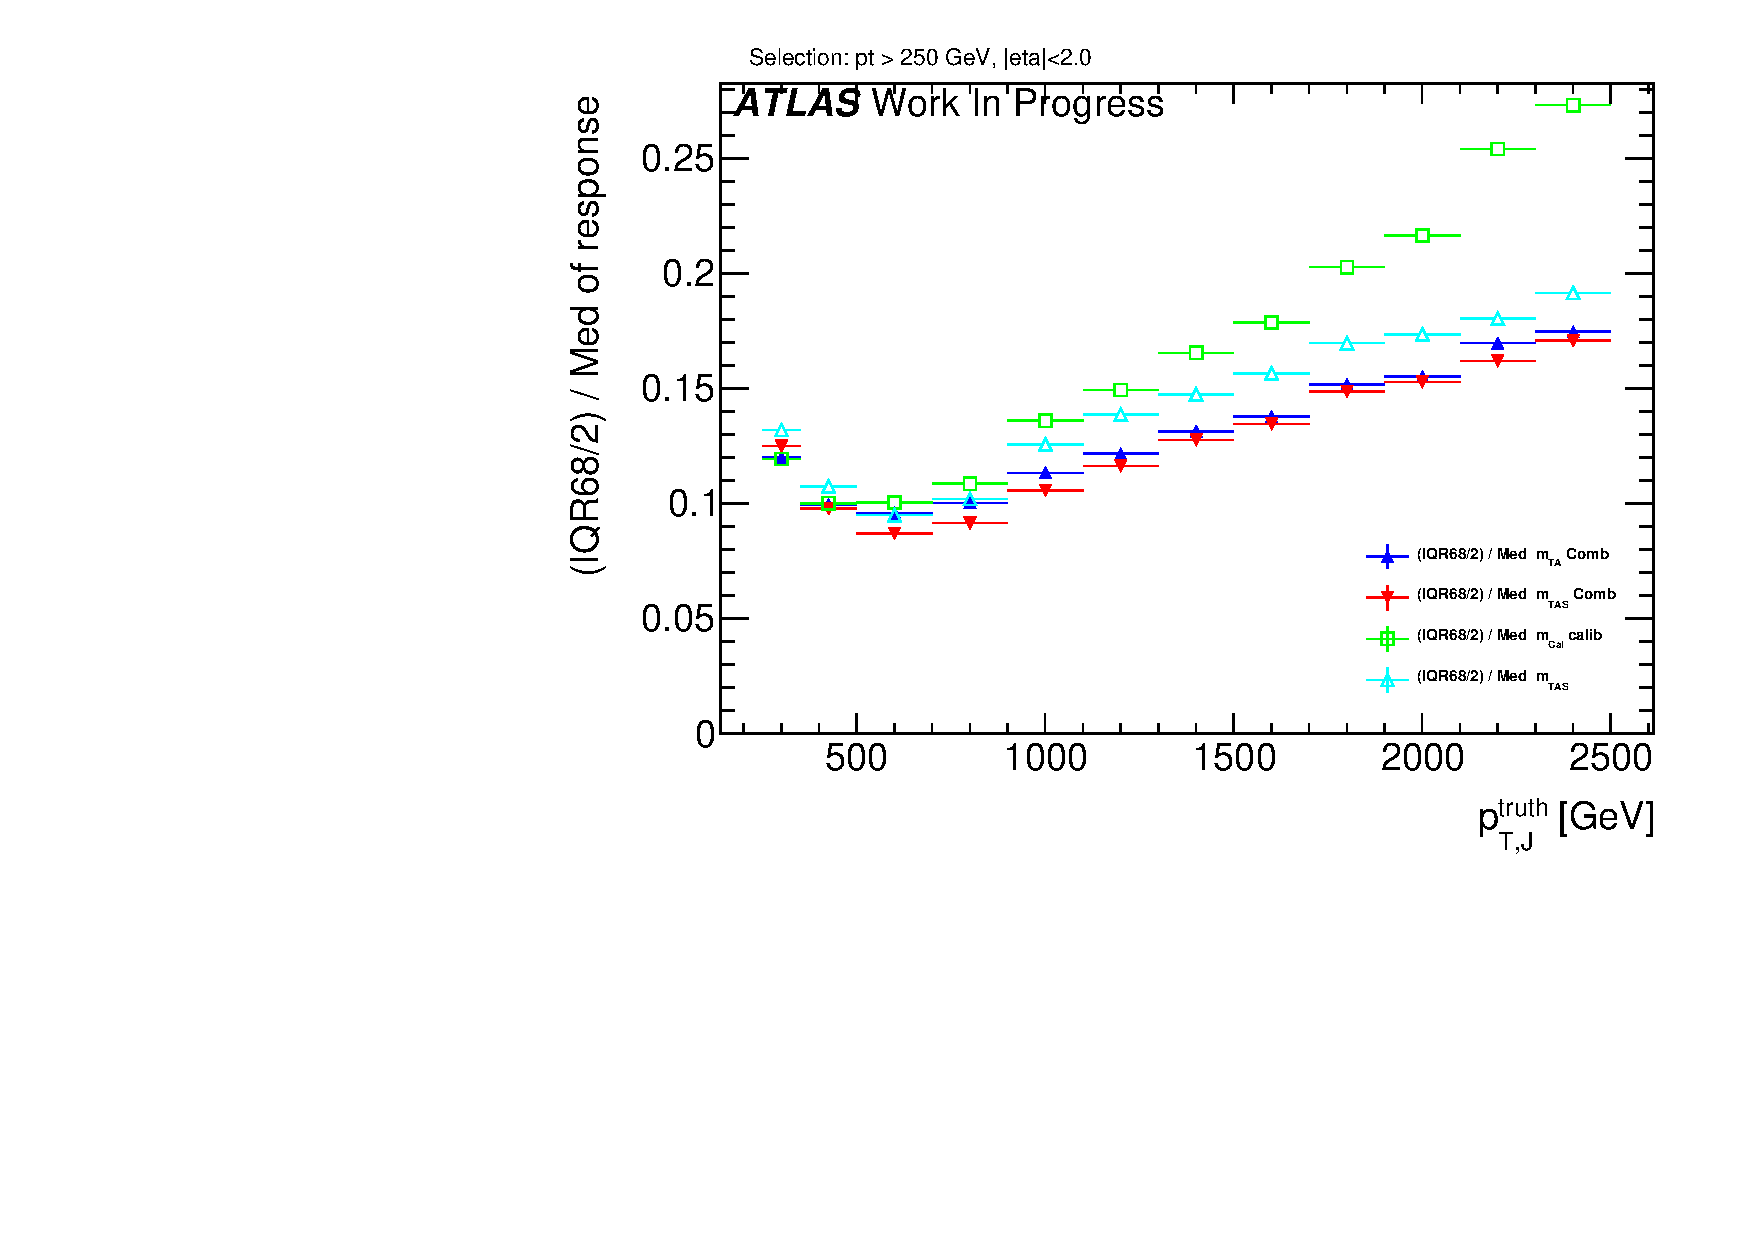
\includegraphics[width=0.7\textwidth]{jet_part/mcomb/mcombtas3.pdf}
  \caption[$\mcombtas$ on the boosted $W/Z$]{Performance of the combined mass on $W/Z$ samples; here shown the two definitions of the combined mass, $\mcomb$ and $\mcombtas$, together with the calorimeter mass and the track-assisted sub-jet mass.}
  \label{fig:mcombtas3}
\end{figure}


\subsection{Performance in $t\to q'\bar{q}b$ Decays}
The boosted top sample remains the most challenging one also with the combined mass; as seen on Figure \ref{fig:mcombtas4}, the $\mcomb$ performs quite similarly to the calorimeter based mass definition, yet behaving considerably better than the $\mtas$ especially at high transverse momentum. The $\mcombtas$, however, outperforms all the other definitions, and shows its optimal observable strength at middle $\pt$ i.e. in the range $1< \pt < 1.6$ TeV.

\begin{figure}[!ht]
  \centering
      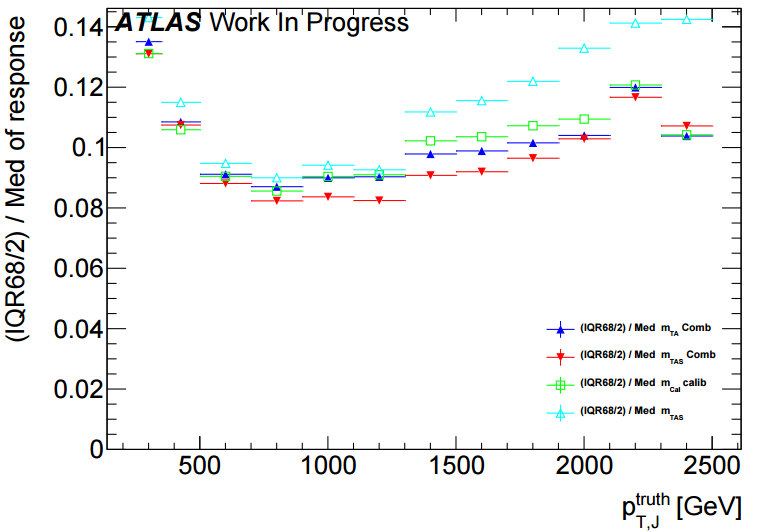
\includegraphics[width=0.7\textwidth]{jet_part/mcomb/mcombtas4.png}
  \caption[$\mcombtas$ on the boosted tops]{Performance of the combined mass on the top sample; here shown the two definitions of the combined mass, $\mcomb$ and $\mcombtas$, together with the calorimeter mass and the track-assisted sub-jet mass.}
  \label{fig:mcombtas4}
\end{figure}

\subsection{Performance in $h\to b\bar{b}$ Decays}
Again, for the Higgs decay there are similarities as for the top sample; on Figure \ref{fig:mcombtas5} the two definitions of the combined mass, together with the simpler $\mtas$. Although this variable is lightly sub-optimal yet still comparable in the low to intermediate range in transverse momenta, where the tracks are driving a decrease in performance for the high to very-high $\pt$. The $\mcombtas$ uses this advantage to achieve optimal behavior in the entire transverse momentum spectrum, outperforming both $\mcal$ and $\mcomb$ almost everywhere.

\begin{figure}[!ht]
  \centering
      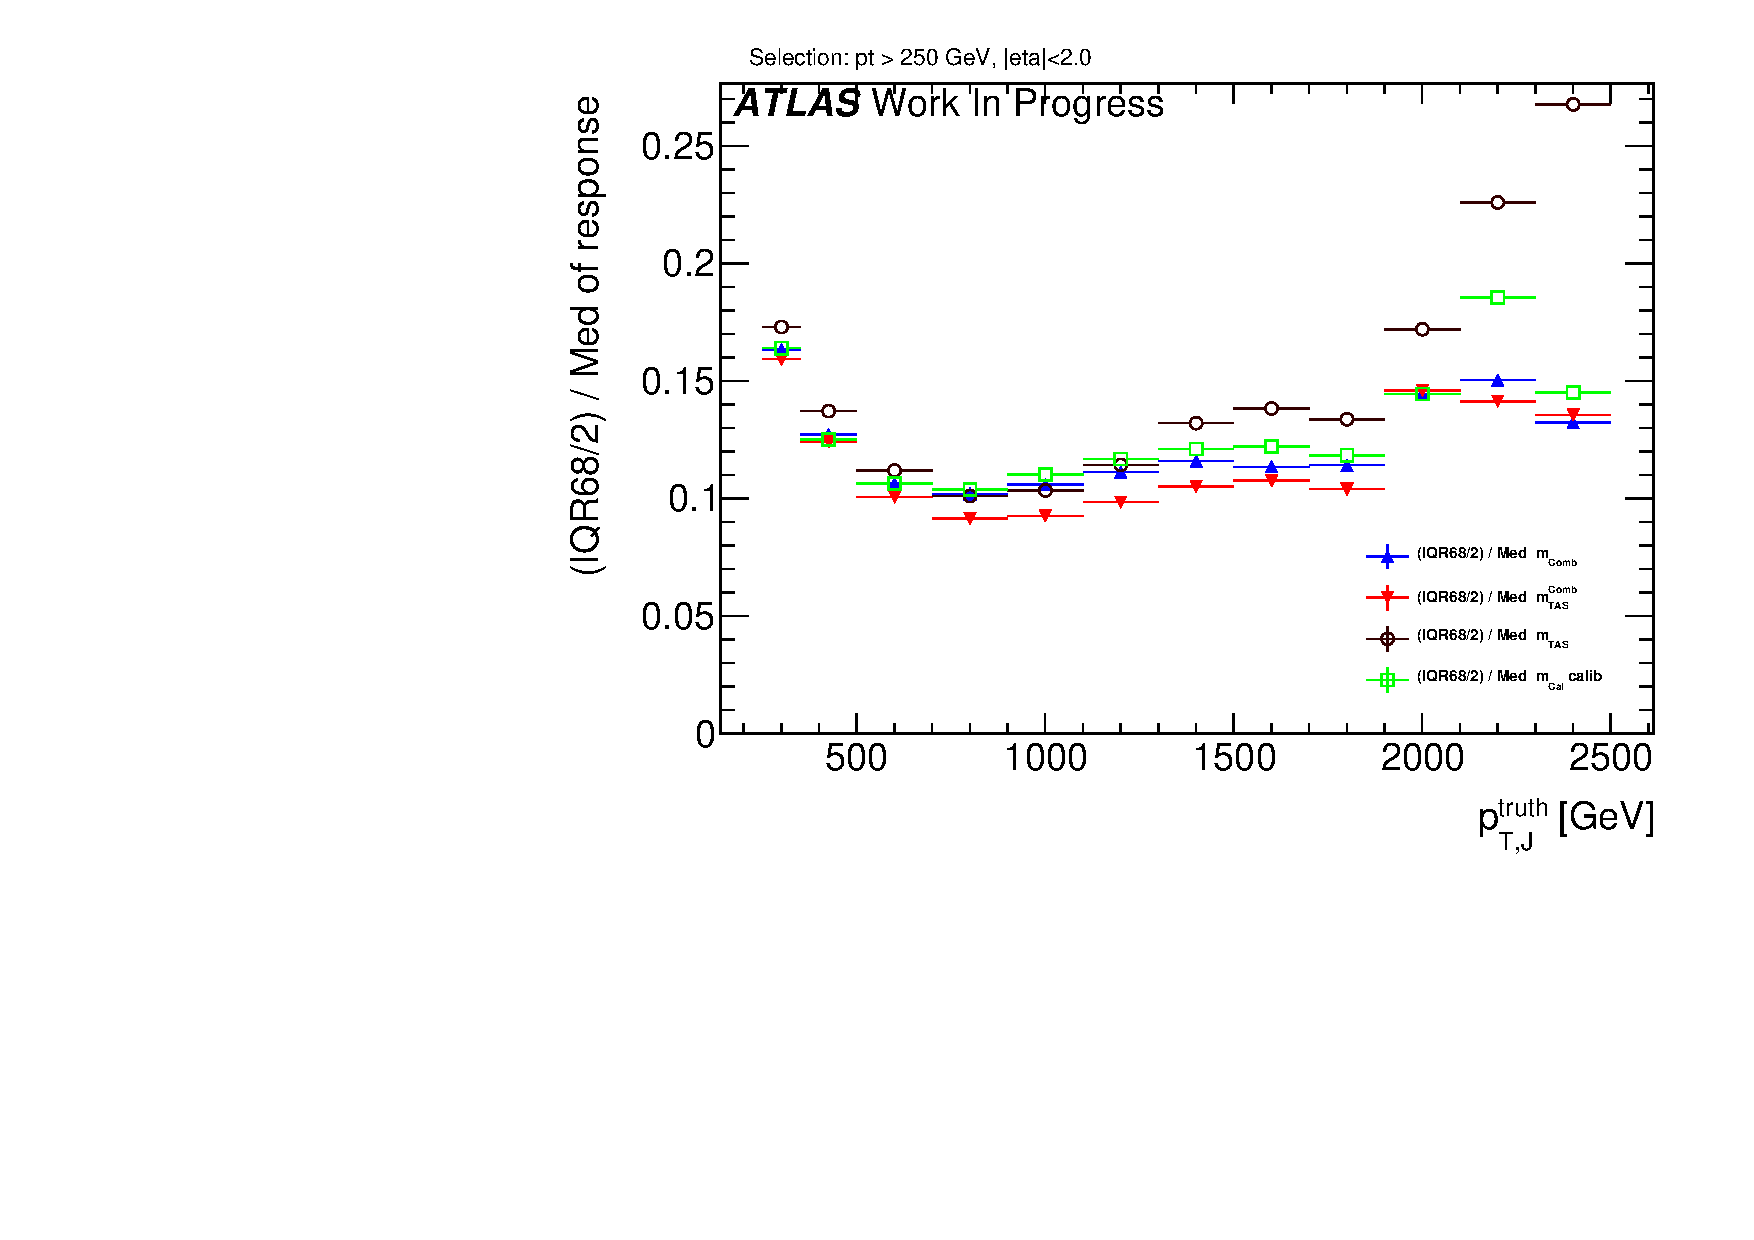
\includegraphics[width=0.7\textwidth]{jet_part/mcomb/mcombtas5.pdf}
  \caption[$\mcombtas$ on the boosted Higgs]{Performance of the combined mass on the Higgs decay; here shown the two definitions of the combined mass, $\mcomb$ and $\mcombtas$, together with the calorimeter mass and the track-assisted sub-jet mass.}
  \label{fig:mcombtas5}
\end{figure}



%-------------------------------------------------------------------------------
\section{Energy Correlation Functions and n-Subjettiness}
Tracks and their angular resolution could not only improve the jet mass definition but also the performance of tagging variables such as the Energy Correlation Functions or n-Subjettiness. These variables are usually calculated with calorimeter clusters as input, studied here are tracks and assisted tracks as input in comparison with the default method using clusters. 
In contrast to the $\mta$ variable introduced in Section \ref{subsec:mta}, not the mass but the $p_{\mathrm{T}}$ of each track is scaled, since C2, D2, $\tau_{21}$ and $\tau_{32}$ are calculated with the constituents $p_{\mathrm{T}}$.

The concept of track assisting with the $p_{\mathrm{T}}$ ratio of the whole jet is without effect for the studied substructure variables. This can be understood from the definitions of the weighted $p_{\mathrm{T}}$ sums. If corrected with only one ratio, all tracks are scaled by the same factor $c$, which then can be put in front of the sum and cancels as soon as the ratios $\tau_{21}$ and $\tau_{32}$, respectively C2 and D2 are formed.
\begin{equation}
\begin{aligned}
 & \tau_N ={} \frac{1}{d_0}\sum_k p_{T,k} \; c \; min(\Delta R_{1,k},\Delta R_{2,k},...,\Delta R_{N,k})^{\beta} \\
 & \; \; \; \;  ={} \frac{c}{d_0}\sum_k p_{T,k}\:min(\Delta R_{1,k},\Delta R_{2,k},...,\Delta R_{N,k})^{\beta}
\end{aligned}
\end{equation}
Track assisting with ghost association to subjets (TAS), see Section \ref{subsec:mtas} for $\mtas$ works with different scaling factors depending on the corresponding sub-jet $c_k$, which also affect ratios:
\begin{equation}
\tau_N = \frac{1}{d_0}\sum_k p_{T,k} \; c_k \; min(\Delta R_{1,k},\Delta R_{2,k},...,\Delta R_{N,k})^{\beta} 
\end{equation}\label{eq:tas_ta}
This leads to the following adaption of the TAS procedure:
\begin{equation}
\begin{pmatrix}
                    m_{track} \\ p_{T,track} \\ \eta_{track} \\  \phi_{track}
                    \end{pmatrix}       \rightarrow \begin{pmatrix}
                    m_{track}  \\ p_{T,track}  \frac{p_{T,sub-jet}}{\sum\limits_{ga\:tracks}p_{T,track}} \\ \eta_{track} \\ \phi_{track}
            
            \end{pmatrix}  
\end{equation}\label{eq:track_tas}
Where the sum combines the $p_{\mathrm{T}}$ of all tracks that are associated to a given sub-jet. 


\subsection{Event weighting and Mass-Cut}
The substructure variables are compared via their QCD (multi-jet) rejection performance. While the $p_{\mathrm{T}}$ distribution of the multi-jet sample falls exponentially, the $p_{\mathrm{T}}$ of the signal samples features characteristic peaks related to the different resonance masses, see Figure \ref{fig:p_T}. To avoid bias in the comparison, the signal sample is given weights sucht that the truth $p_{\mathrm{T}}$ distribution of the leading jet matches the one of the background sample. Furthermore, the spectrum is split into six different $p_{\mathrm{T}}$ regions to study the behavior with rising energy. 
\begin{figure} 
	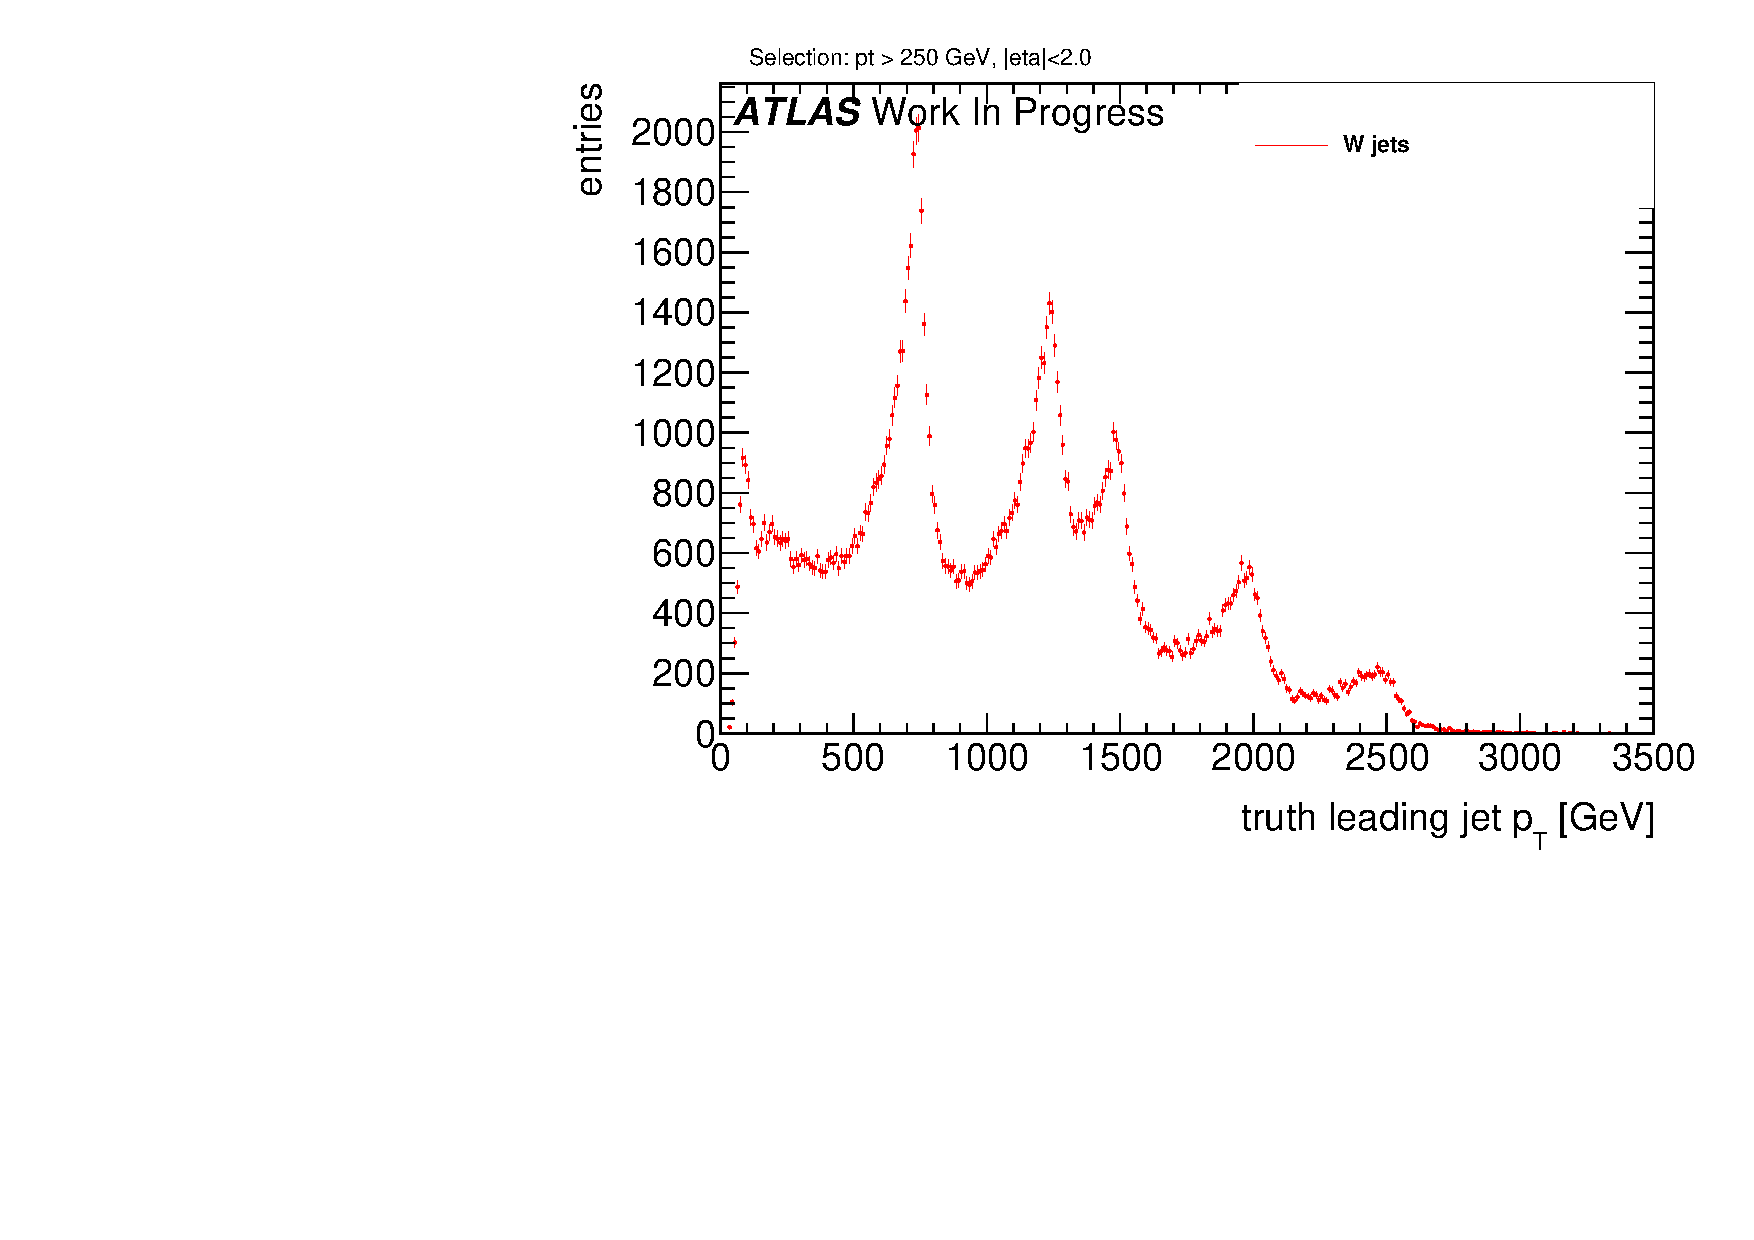
\includegraphics[width=0.5\textwidth]{sascha_input/plots/track_selection/h_leadpt_truth.pdf} \hspace{1mm}
	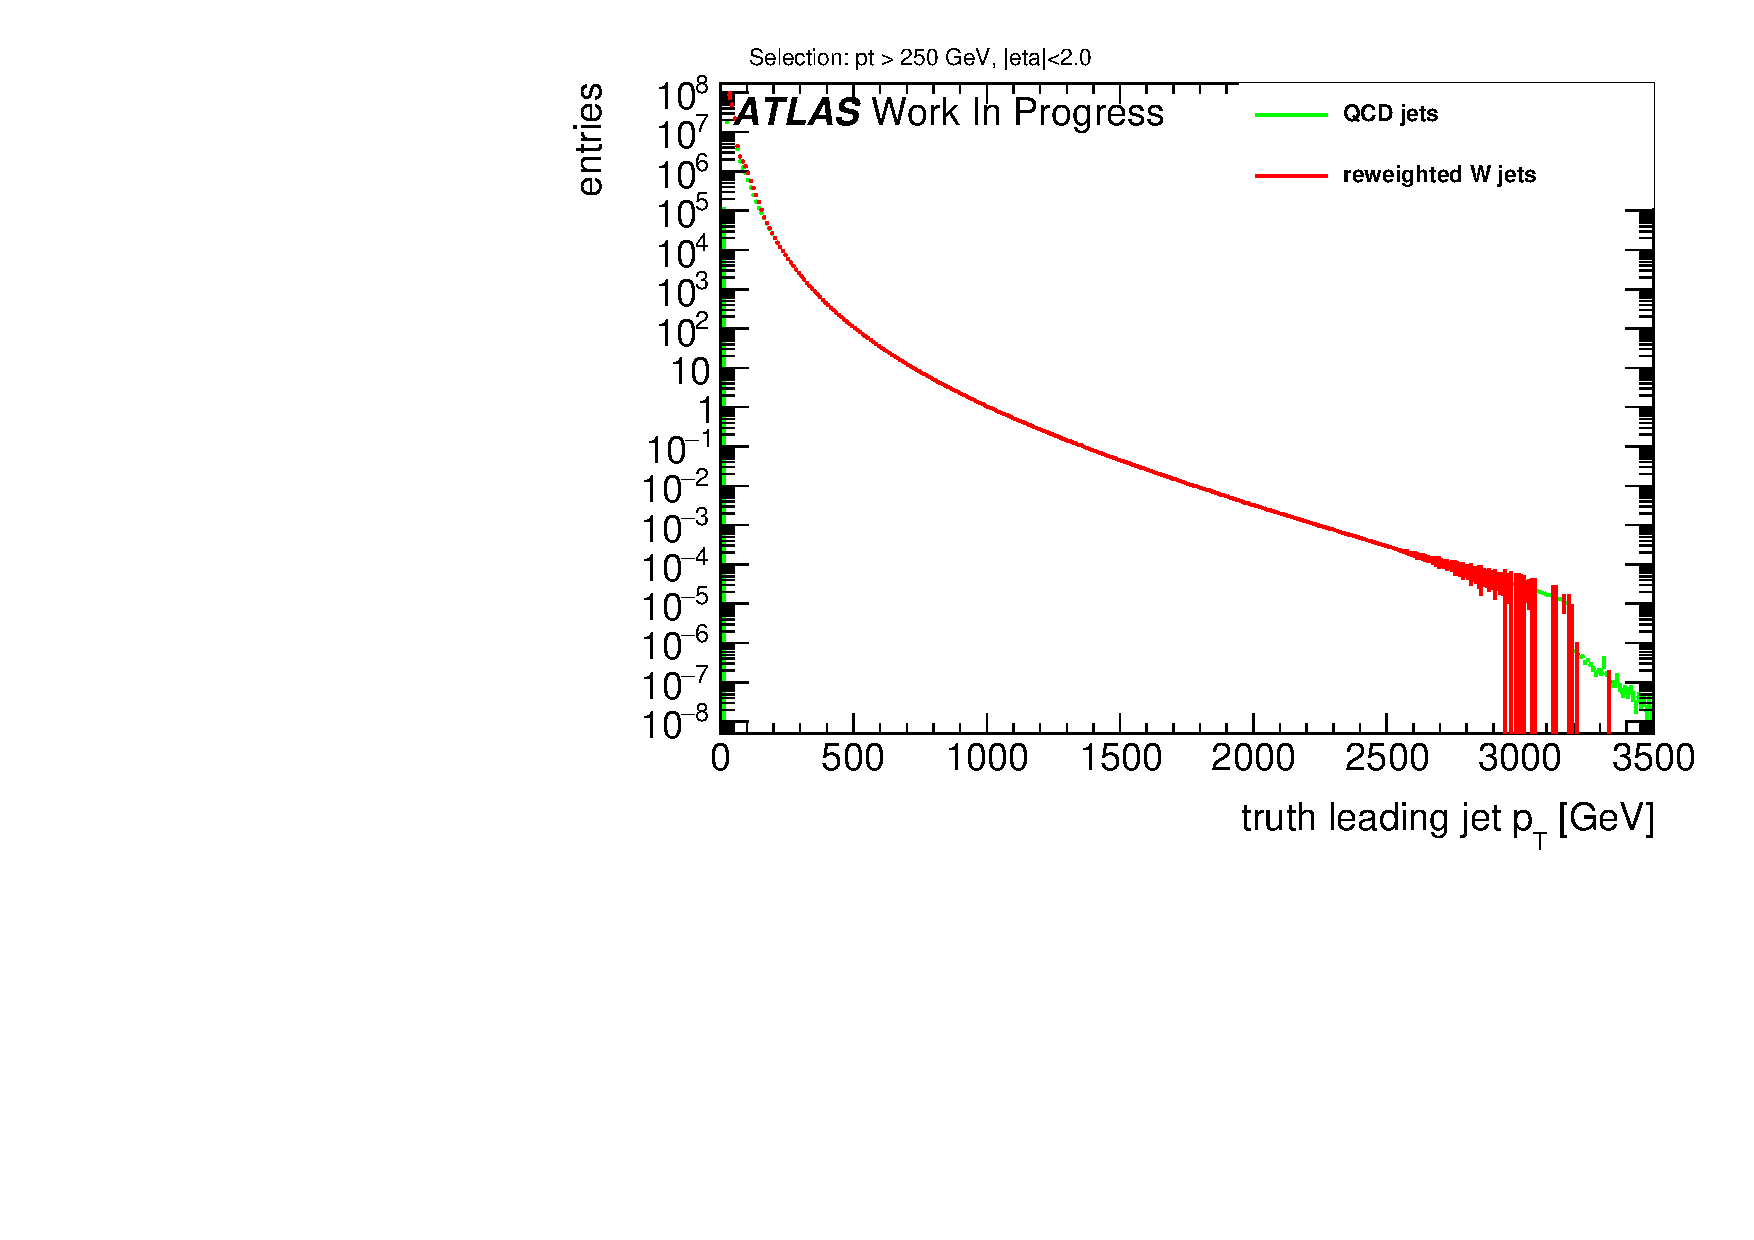
\includegraphics[width=0.5\textwidth]{sascha_input/plots/track_selection/h_leadpt_truth_weight.pdf}
\caption{\footnotesize{Exemplary $p_{\mathrm{T}}$ distributions of (left) $W$ boson jets and (right) QCD jets from multi-jet events with reweighted $W$ boson events}}\label{fig:p_T}
\end{figure}

Tagging variables such as C2, D2, $\tau_{21}$ and $\tau_{32}$ are usually used after applying a mass cut around the interval that contains 68\% of the signal events. Therefore, a cut is applied on the calibrated mass of the large-R calorimeter jet which is calculated to cover the smallest interval around the peak mass that contains 68\% of the signal events.
The comparison is performed in six different $p_{\mathrm{T}}$ regions to study the behavior connected with rising energy of the decaying particle. These regions are presented in the left part of Table \ref{table:mass_cut}. 
In case of the Higgs boson study, there is not enough statistics to derive a conclusive result for $p_{\mathrm{T}} > 2000 \, \text{GeV}$, since the highest resonance mass of the $G^* \rightarrow HH$ samples is $3000 \, \text{GeV}$ in contrast to $5000 \, \text{GeV}$ for the $Z^\prime \rightarrow tt$ and $W^\prime \rightarrow WZ$ samples. Hence this study is restricted to the five lower $p_{\mathrm{T}}$ bins.
Prior to tagging with the n-Subjettiness or C2/D2 variables, a cut on the calibrated calorimeter jet mass is applied, given that the mass is the main discriminant in QCD jet rejection. This cut is defined to choose the smallest interval around the peak mass containing 68\% of the signal. However, the reconstructed mass depends on the $p_{\mathrm{T}}$ region, therefore a different cut was calculated for every region to meet the requirements.
\begin{table}[]
\centering
\begin{tabular}{l||ll||ll||ll}
  &  \textbf{W boson}                                                    &                                 &  \textbf{Higgs boson}                                  &                                &    \textbf{Top quark}                                  &                                  \\ \hline
$p_{\mathrm{T}} \, \text{[GeV]}$   & \multicolumn{1}{l|}{Mass [GeV]} & $\frac{1}{\epsilon_{bgr}}$ & \multicolumn{1}{l|}{Mass [GeV]} & $\frac{1}{\epsilon_{bgr}}$ & \multicolumn{1}{l|}{Mass [GeV]}  & $\frac{1}{\epsilon_{bgr}}$ \\ \hline \hline
250 - 500 & \multicolumn{1}{l|}{63 - 85}                        & 10.8                            & \multicolumn{1}{l|}{56 - 167}          & 3.8                             & \multicolumn{1}{l|}{77 - 191}          & 6.3                             \\ \cline{1-7} 
500 - 800 & \multicolumn{1}{l|}{72 - 92}                        & 13.6                            & \multicolumn{1}{l|}{92 - 150}          & 7.3                             & \multicolumn{1}{l|}{117 -205}          & 6.9                             \\ \cline{1-7} 
800 - 1200 & \multicolumn{1}{l|}{76 - 104}                       & 9.6                             & \multicolumn{1}{l|}{98 - 143}          & 9.5                             & \multicolumn{1}{l|}{122 - 218}         & 6.5                             \\ \cline{1-7} 
1200 - 1600 & \multicolumn{1}{l|}{77 - 107}                       & 7.3                             & \multicolumn{1}{l|}{103 - 149}         & 9.0                             & \multicolumn{1}{l|}{122 - 227}         & 6.3                             \\ \cline{1-7} 
1600 - 2000 & \multicolumn{1}{l|}{79 - 115}                       & 5.6                             & \multicolumn{1}{l|}{91 - 170}          & 4.4                             & \multicolumn{1}{l|}{121 - 235}         & 5.6                             \\ \cline{1-7} 
$> 2000$ & \multicolumn{1}{l|}{80 - 126}                       & 4.2                             & \multicolumn{1}{l|}{/}                 & /                               & \multicolumn{1}{l|}{123 - 251}         & 4.8                             \\ \hline
\end{tabular}
\caption{\footnotesize{Studied $p_{\mathrm{T}}$ regions and corresponding calculated 68\% mass intervals along with the background rejections from the mass cut for $W$ boson, Higgs boson and Top quark jets.}} \label{table:mass_cut}
\end{table} 




\subsection{Track Selection}
There are different collections of tracks that could be used to calculate substructure variables. Compared here are tracks that are ghost associated to the ungroomed large-R jet with the collection which is also used for the $\mtas$, see Section \ref{subsec:ObsDef_Proc}, which is ghost association to $k_T$-subjets and $\Delta R$ matching of tracks close to sub-jets.

The distributions showing the number of tracks associated to a calorimeter jet, see the left side of Figure \ref{fig:delta_R}, indicate, that on average around four tracks less are associated to the sub-jets compared to the ungroomed jet. The right side of Figure \ref{fig:delta_R} shows the angular distance $\Delta R$ between the single tracks and the axis of the large-R calorimeter jet. Both distributions are aligned in the lower $\Delta R$ region while the histogram representing the tracks associated to the ungroomed jet shows an enhancement towards larger $\Delta R$. Accordingly, these additional tracks feature an angular separation from the jet axis of more than $0.3$, and are in consequence distributed primarily around the outer regions of the large-R jet. Given the required primary vertex association, it is unlikely that these tracks originate from pile-up. Instead, the origin might be found in final- or initial state radiation. 
\begin{figure}
	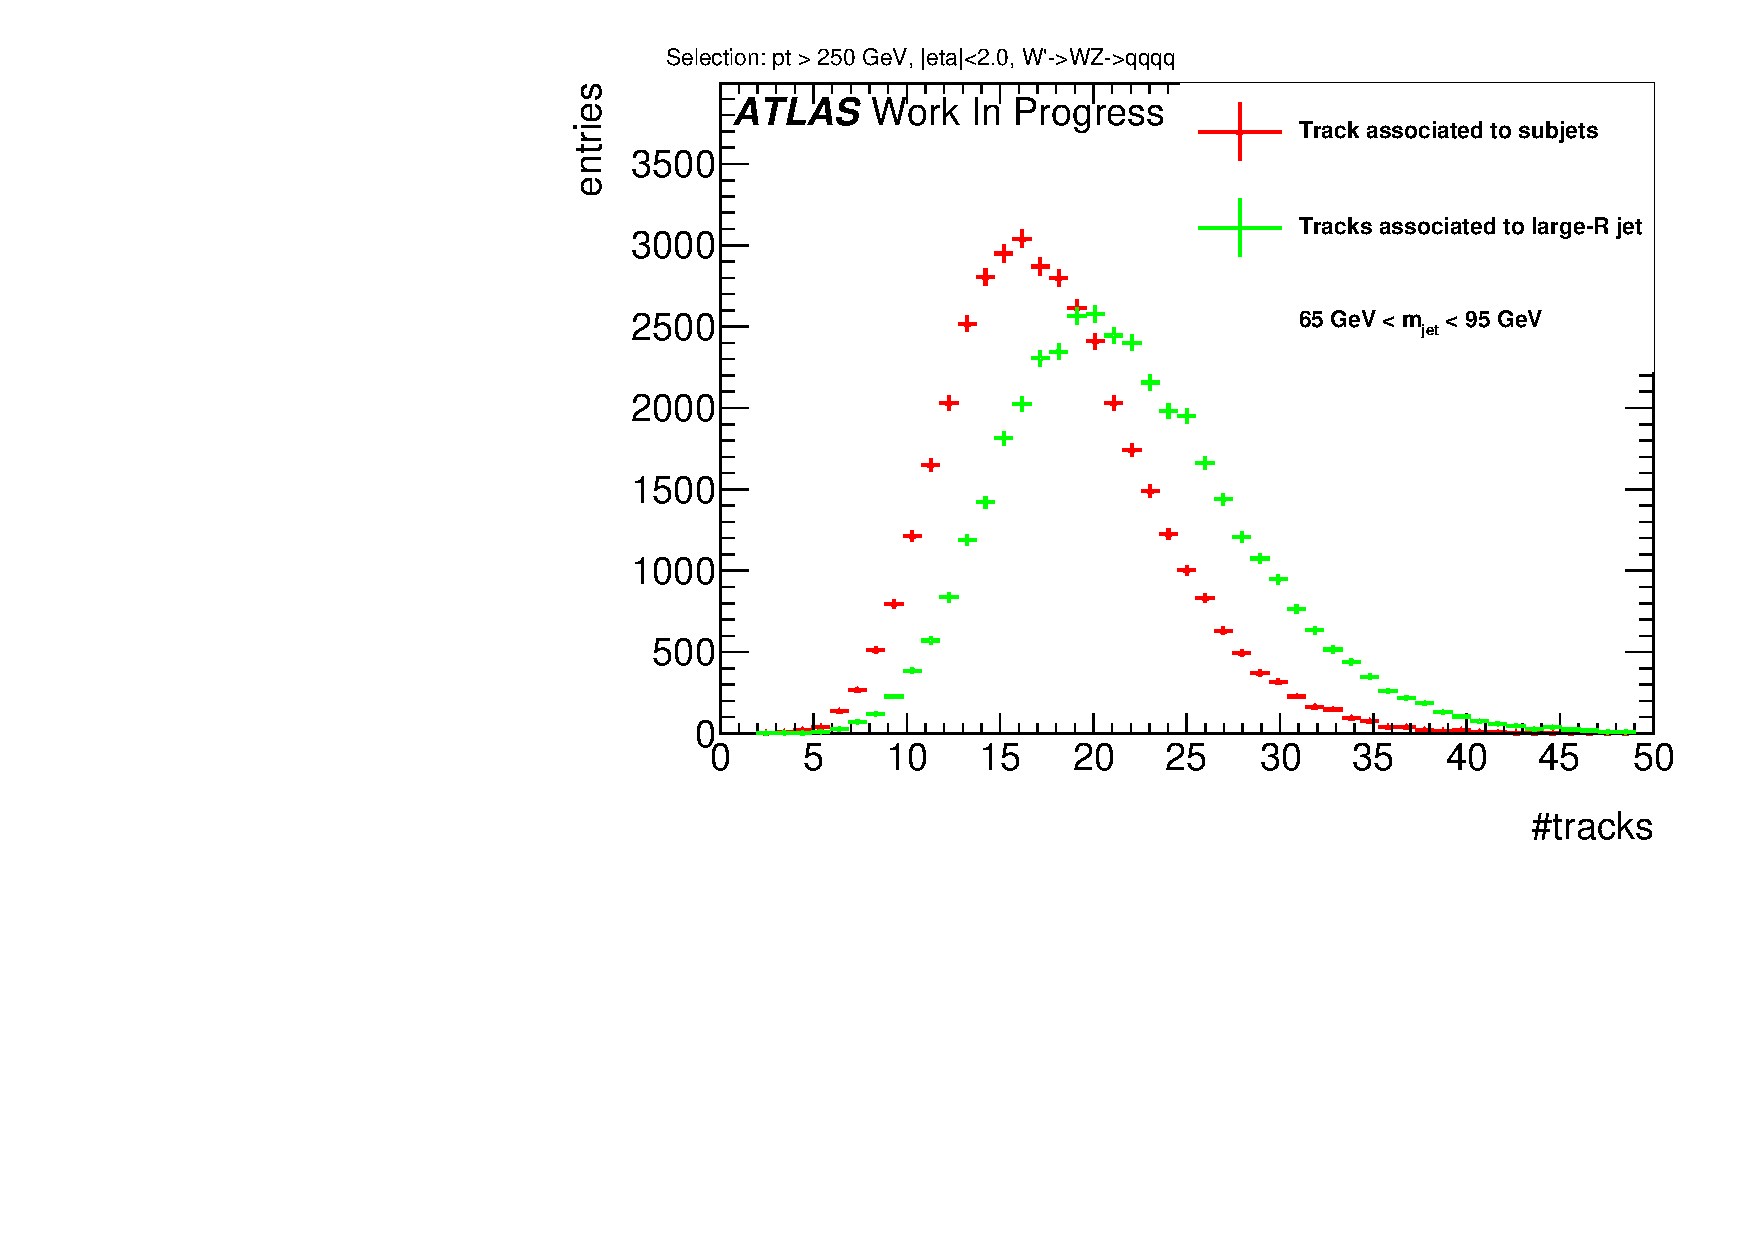
\includegraphics[width=0.5\textwidth]{sascha_input/plots/track_selection/h_customghost_number.pdf} \hspace{1mm}
	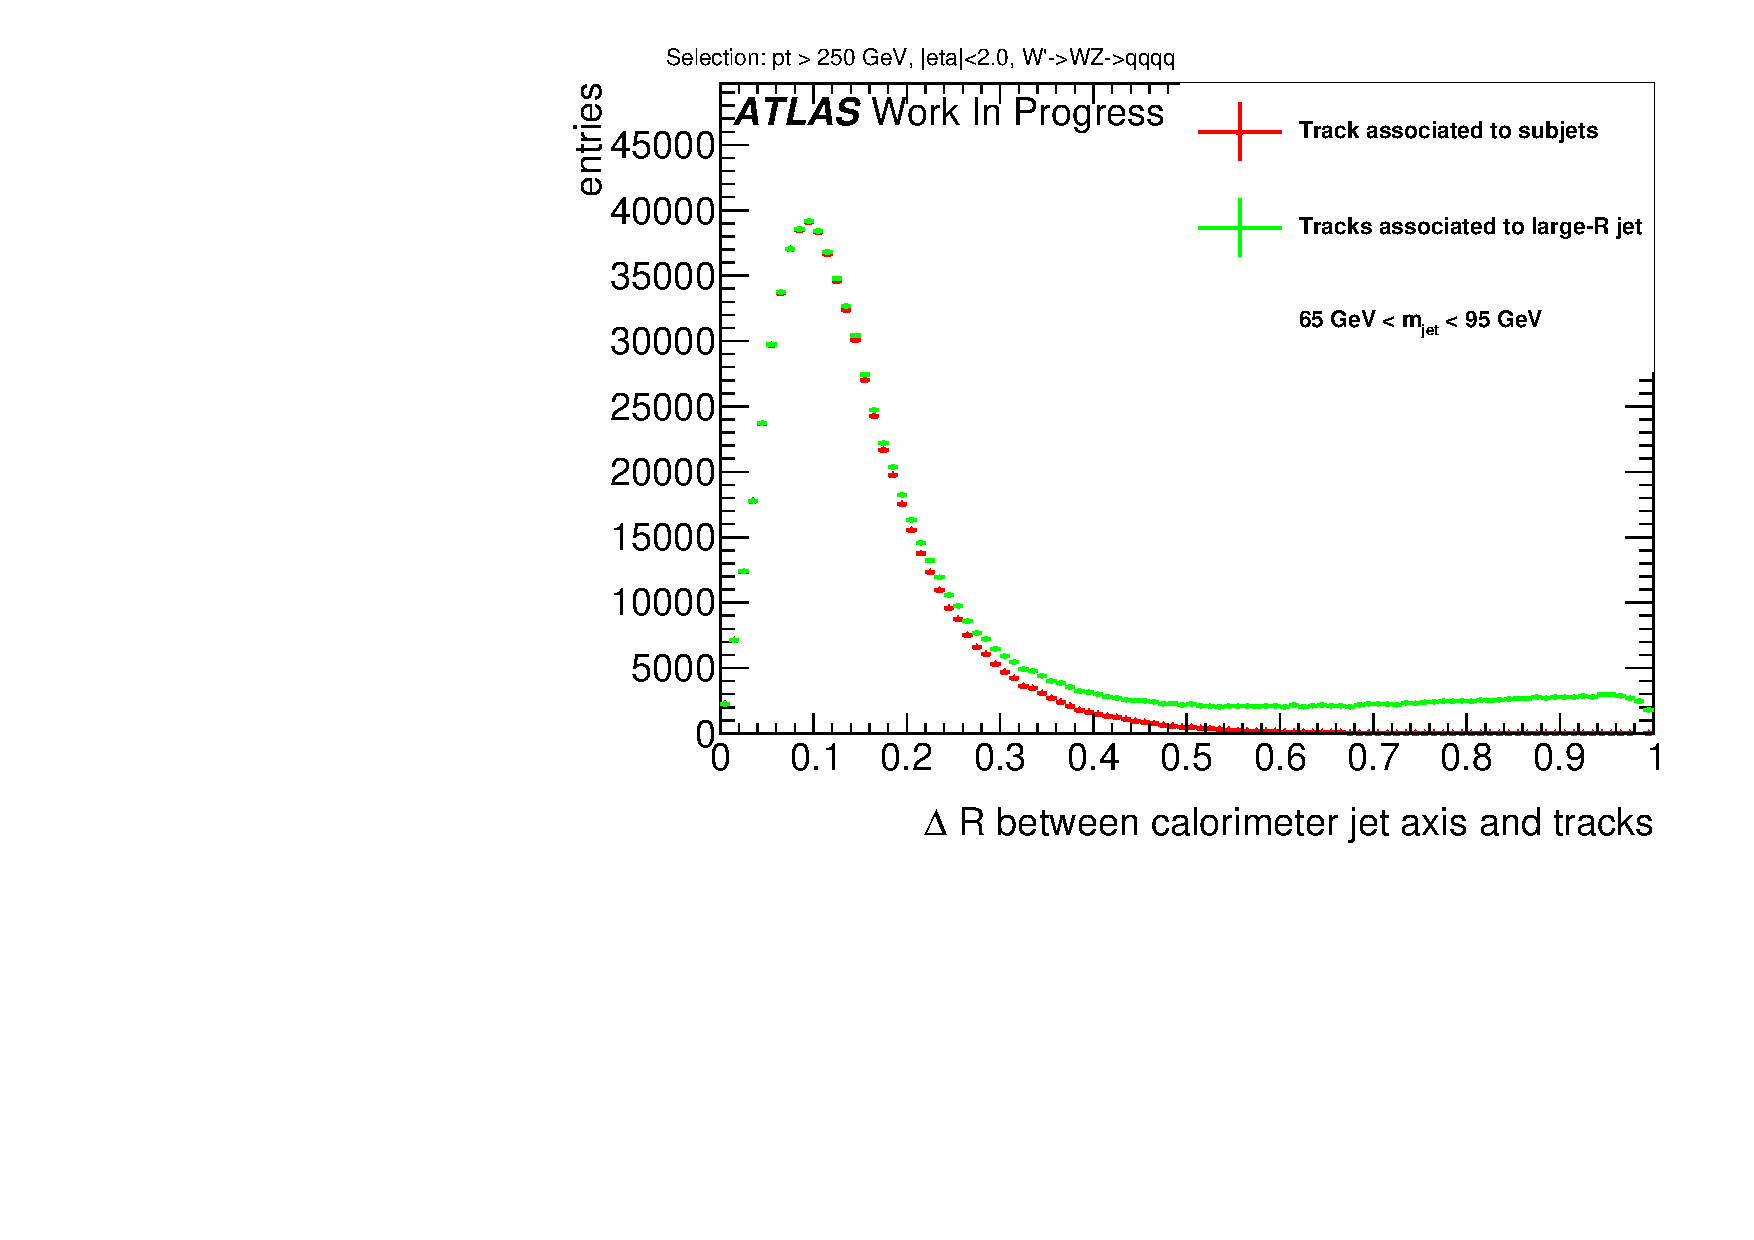
\includegraphics[width=0.5\textwidth]{sascha_input/plots/track_selection/h_customghost_dr.pdf}
\caption{\footnotesize{The number of tracks ghost associated to the large-R jet and to the sub-jets (left) and angular distance of associated tracks to the large-R calorimeter jet axis (right). Signal events were not reweighted at this step.}}\label{fig:delta_R}
\end{figure}

Figure \ref{fig:selection} shows the signal distributions of the C2/D2, and $\tau_{21}$, calculated with both selections of tracks for $W$ boson jets. The large $\Delta R$ to the jet axis of the differing tracks push the substructure variables to higher, more background like values. The broader distributions are a result of the variating nature of these tracks. C2 and D2 are more sensitive to tracks with a large $\Delta R$ to the jet axis, because the angular distance between all pairs and triples of tracks is considered, among tracks on possibly opposite ends of the large-R jet, whereas $\tau_{21}$uses distances to $k_\mathrm{T}$-WTA axes.
\begin{figure}
	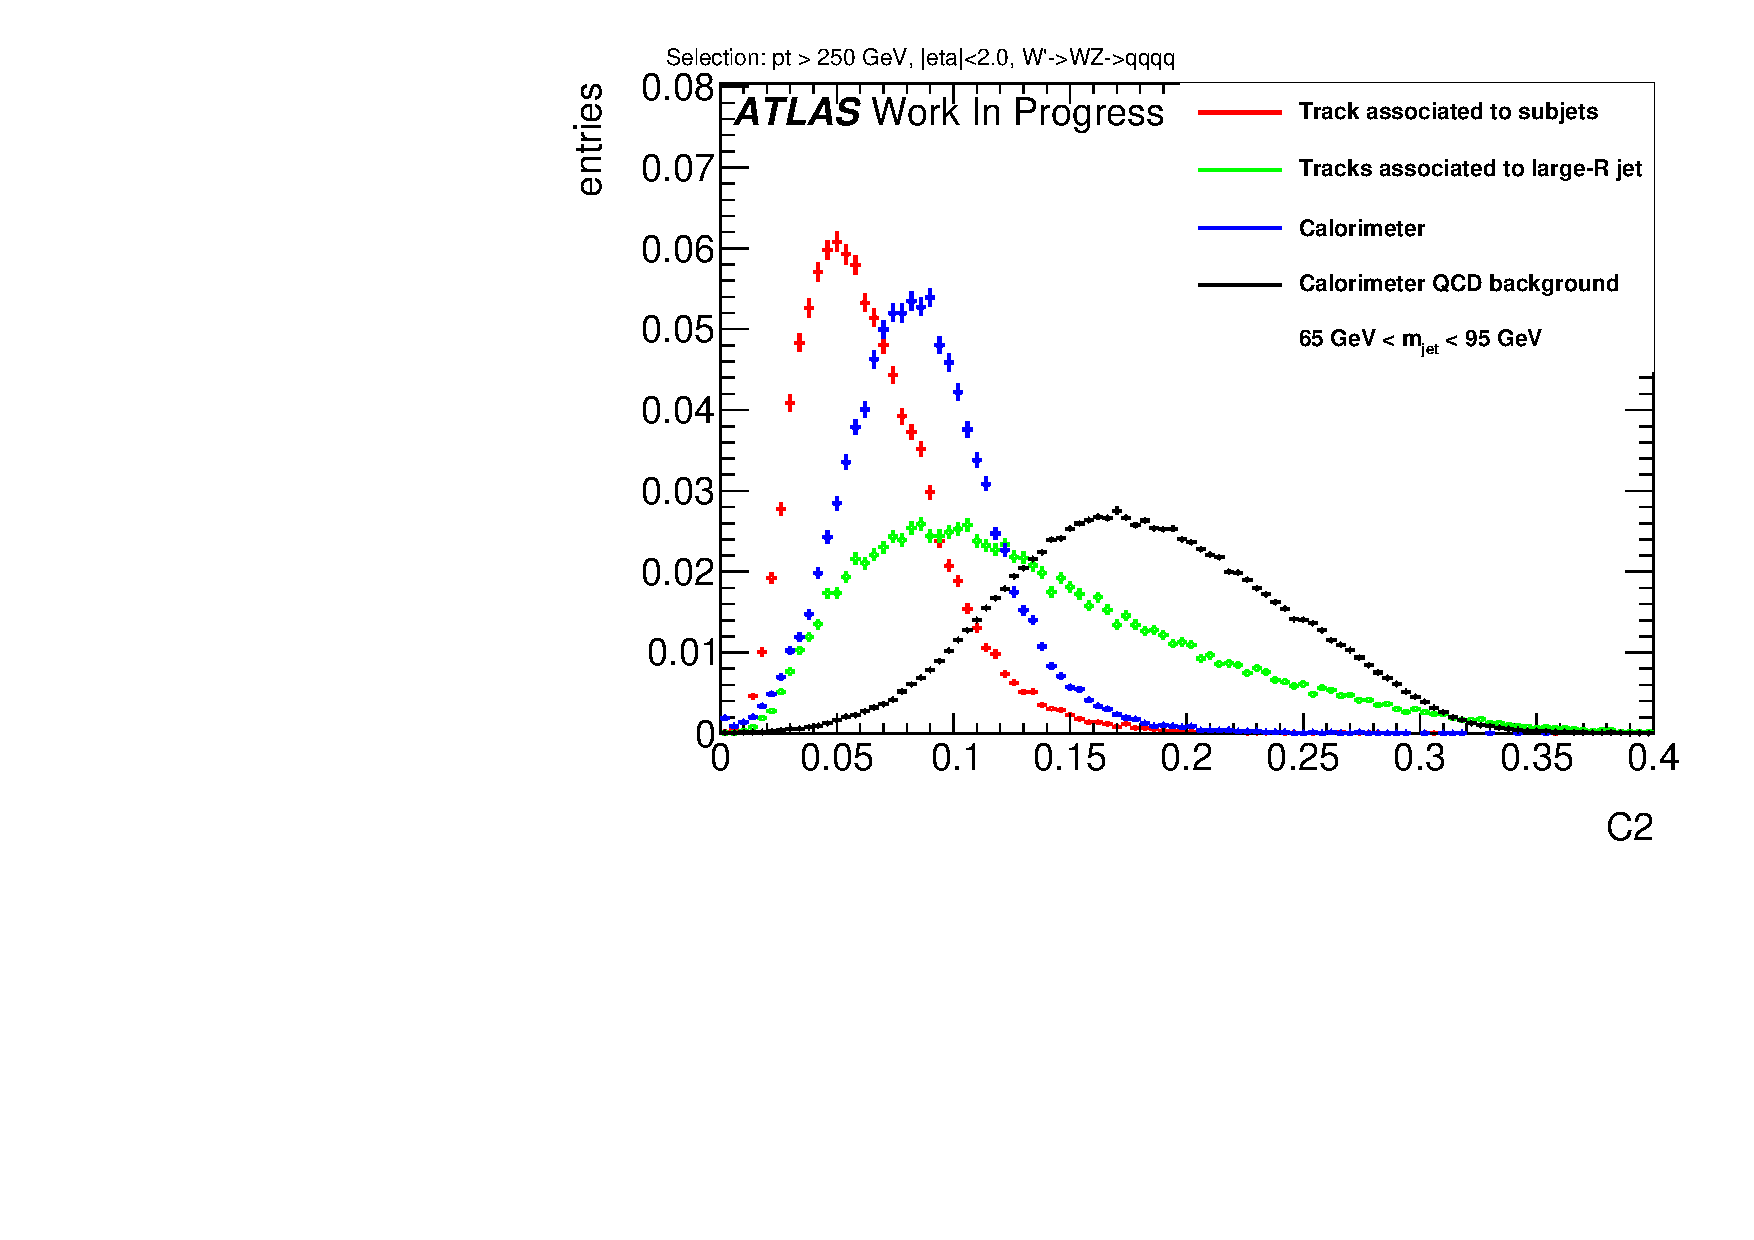
\includegraphics[width=0.45\textwidth]{sascha_input/plots/track_selection/h_ghost_sj_C2.pdf} \hspace{1mm}
	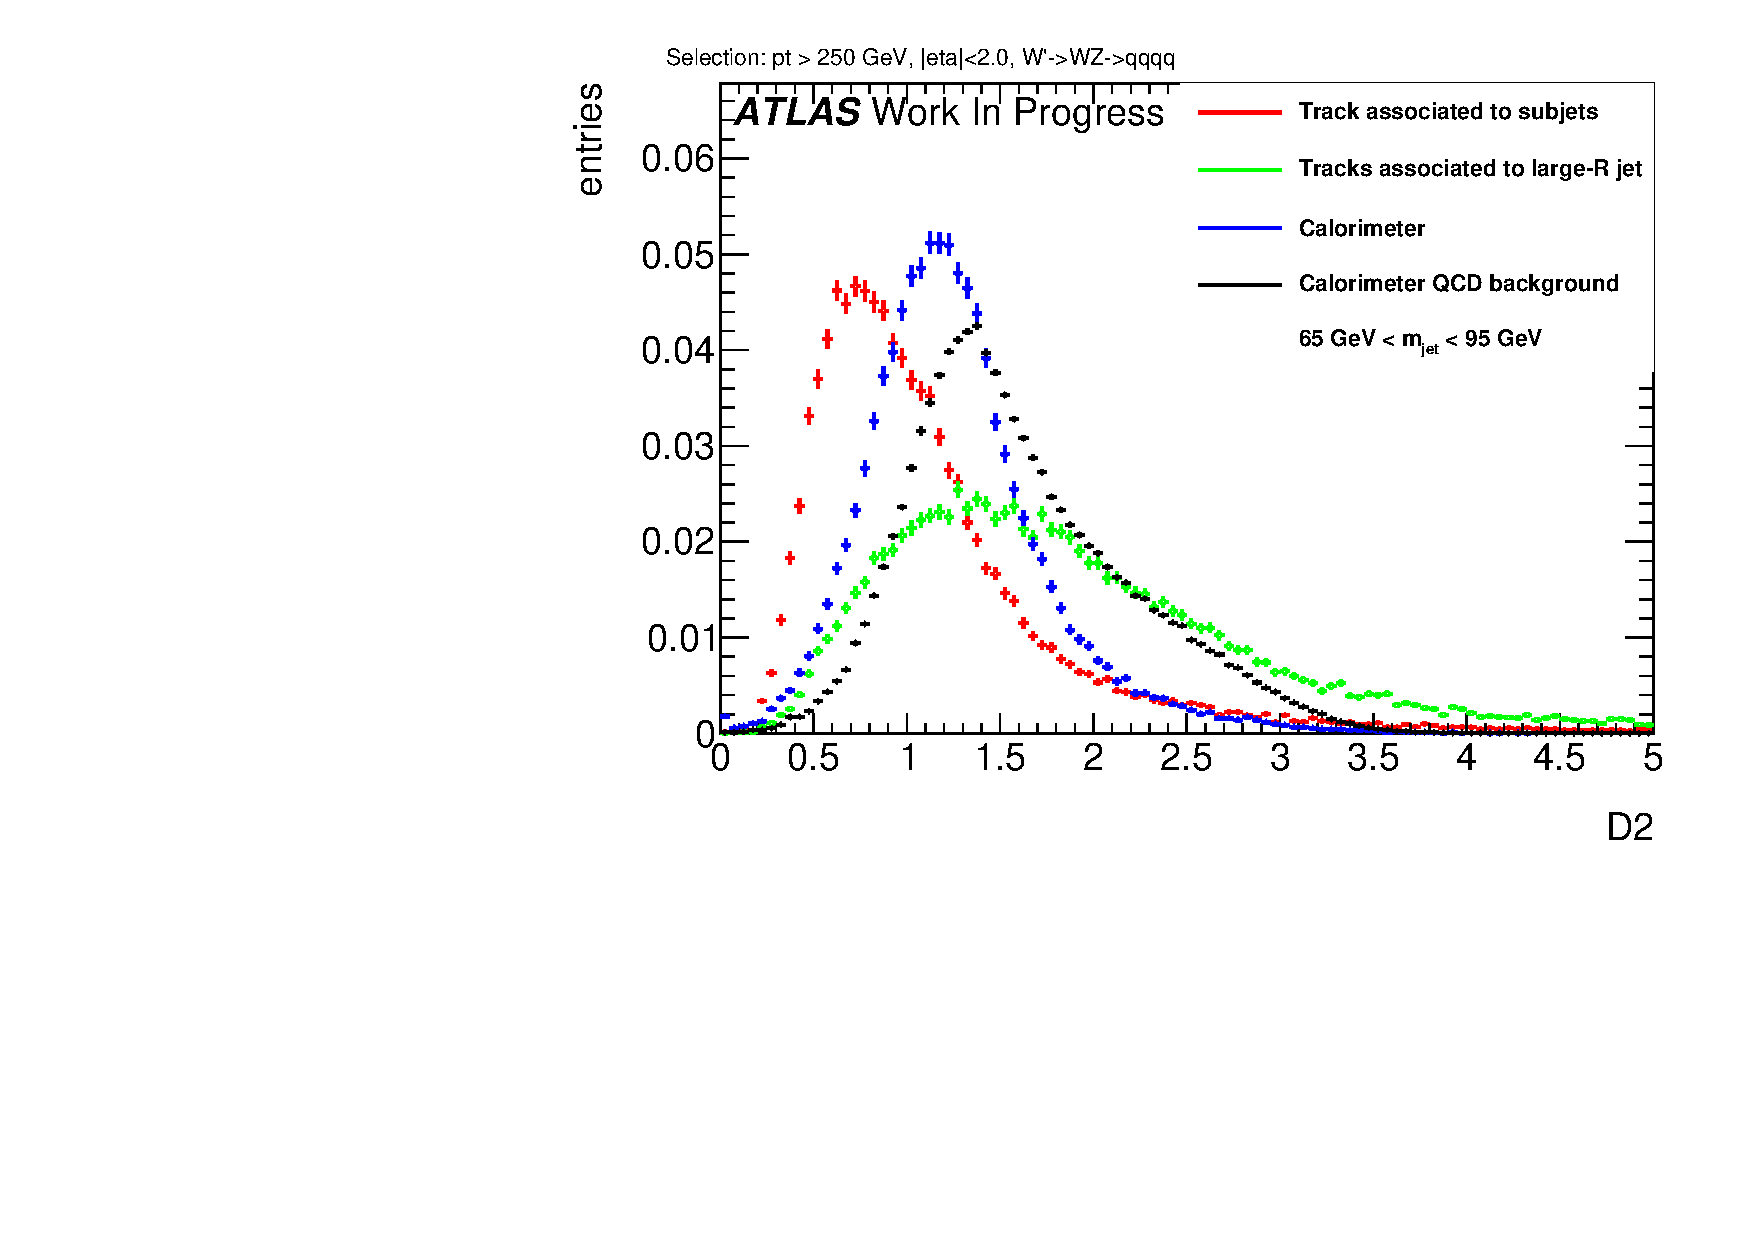
\includegraphics[width=0.45\textwidth]{sascha_input/plots/track_selection/h_ghost_sj_D2.pdf}
	\bigskip
	\centering
	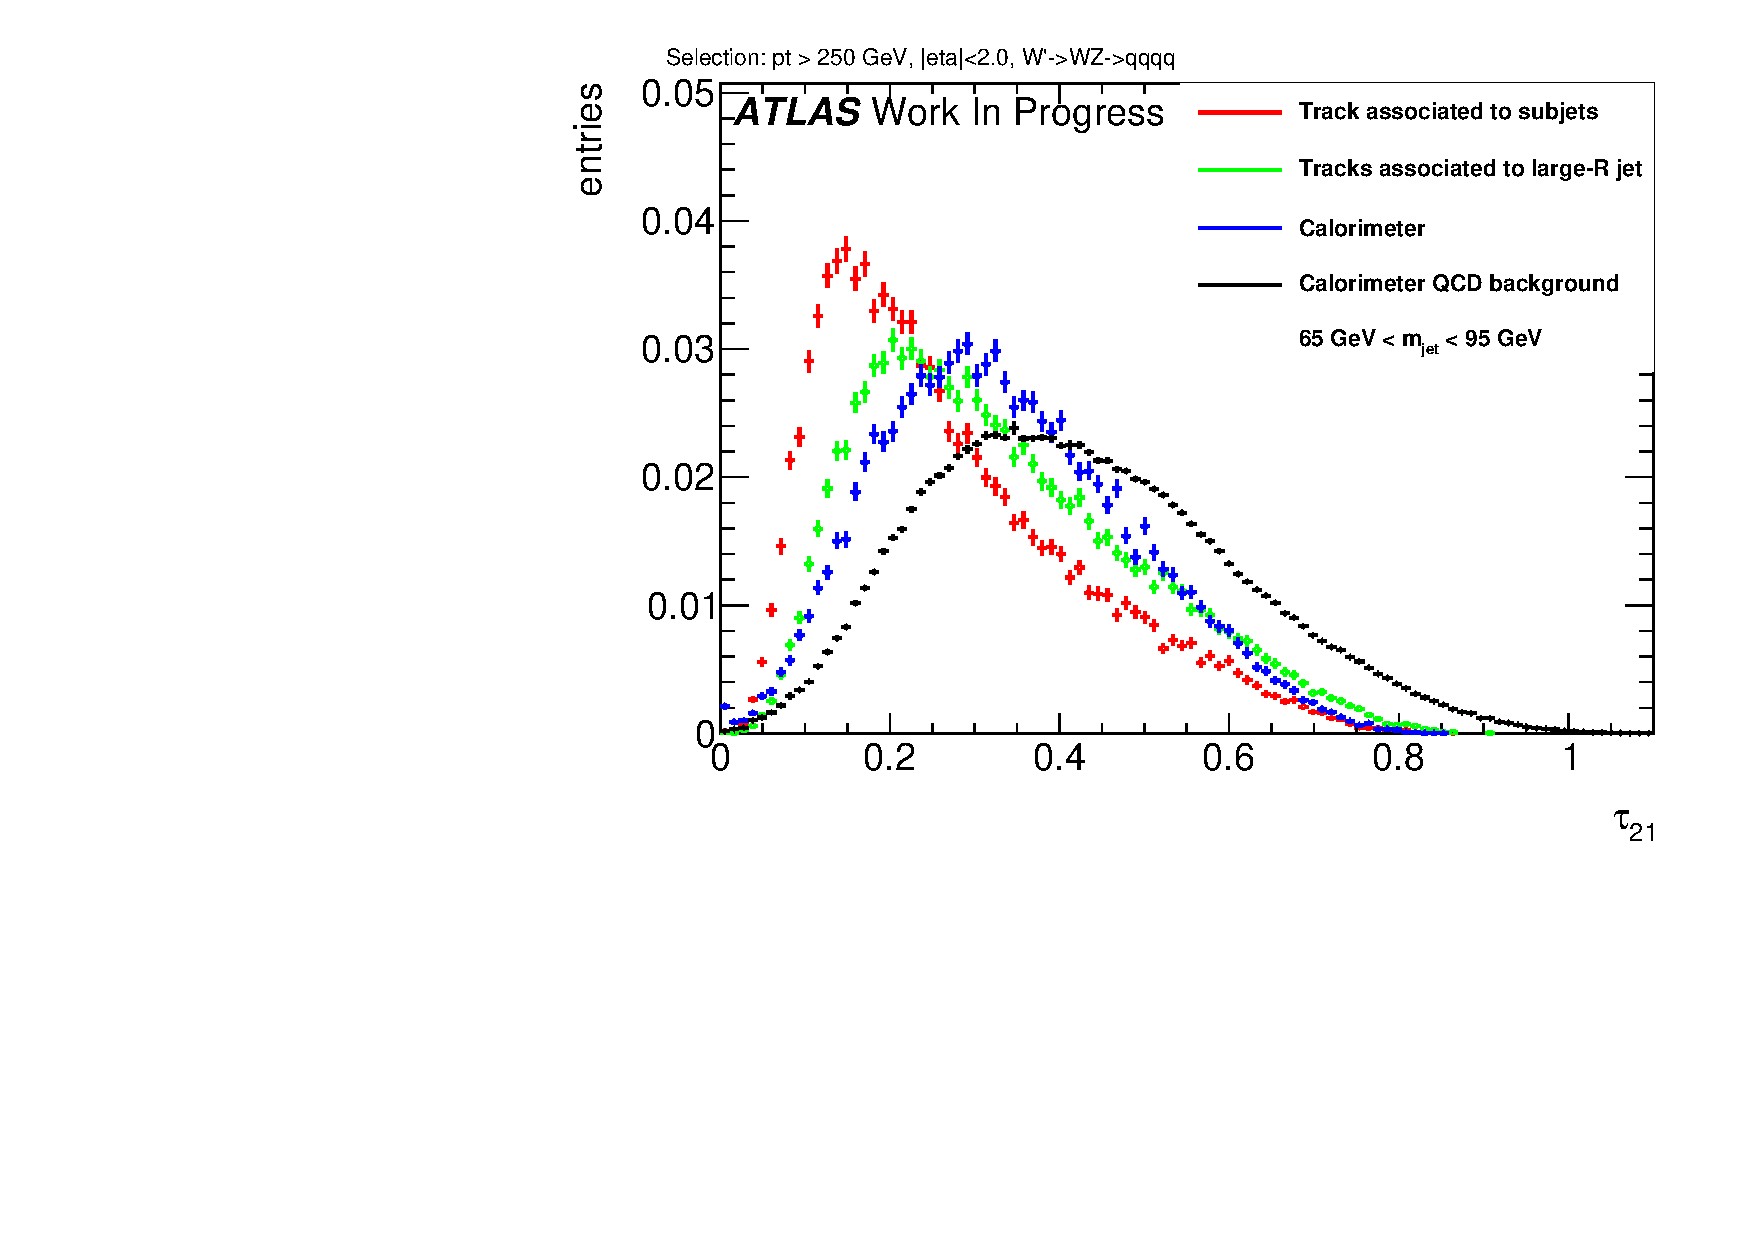
\includegraphics[width=0.45\textwidth]{sascha_input/plots/track_selection/h_ghost_sj_nSub21.pdf}
\caption{\footnotesize{Substructure variables (left) C2, (right) D2 and (below) $\tau_{21}$ calculateated with calorimeter clusters as well as tracks associated to sub-jets and to the large-R jet. Signal events were not reweighted at this step.}}\label{fig:selection}
\end{figure}
For comparison, the signal and background distributions for the variables calculated with calorimeter clusters are shown as well. It is possible to anticipate that the performance of variables calculated with tracks and assisted tracks is not worse than cluster base variables.
In contrast to the previously studied jet mass variable, ratios of ECF(N) and $\tau_N$ are rather energy scale independent and are found to not be as sensitive to the missing neutral fraction with un-assisted tracks.
Starting from this observations, the performance of substructure techniques is compared with the following objects as input:
\begin{itemize}
\item Calorimeter clusters, labeled 'calo'.
\item Tracks selected as described in Section \ref{subsec:ObsDef_Proc}, labeled 'tracks'.
\item The same collection of tracks, assisted as defined in Section \ref{subsec:ta_adapt}, labeled 'TAS'.
\end{itemize}

\subsection{Performance with default $\beta$}

The performance of track and TAS based tagging variables with the default angular weighting of $\beta=1$ is compared to the corresponding calorimeter variables for $W$ boson, Higgs boson and Top quark identification. 
The stated signal efficiencies are calculated after the mass cut plus tagging with n-Subjettiness or C2/D2. Therefore, the endpoint of the ROCs is at 68\% signal efficiency, the fraction kept after the mass cut. Consequently, it is required to achieve a tagging only signal efficiency of $\frac{0.5}{0.68} \sim 0.74$ for a signal efficiency of 0.5 after mass cut and tagging. Similarly, the stated and compared background rejections result from the multiplication of both, thus representing the QCD rejection of the combined mass- and tagging variable-cut. 
The complete set of signal and background distributions for different inputs can be found in the Appendix \ref{app:sascha}.

\subsubsection{Performance for $W$ boson tagging}
Shown in Figure \ref{fig:w_distribution_example} are exemplary signal and background distributions in intermediate $p_T$ bins compared for different inputs. This shows throughout narrower signal distributions rising slightly sharper for tracks and assisted tracks compared to calorimeter clusters which can be explained by the high angular resolution. The right handed tails of the signal distributions are similar to the calorimeter variables. Similarly, the background distributions shift as well, but not as distinct as seen for the signal.
\begin{figure}[htp]
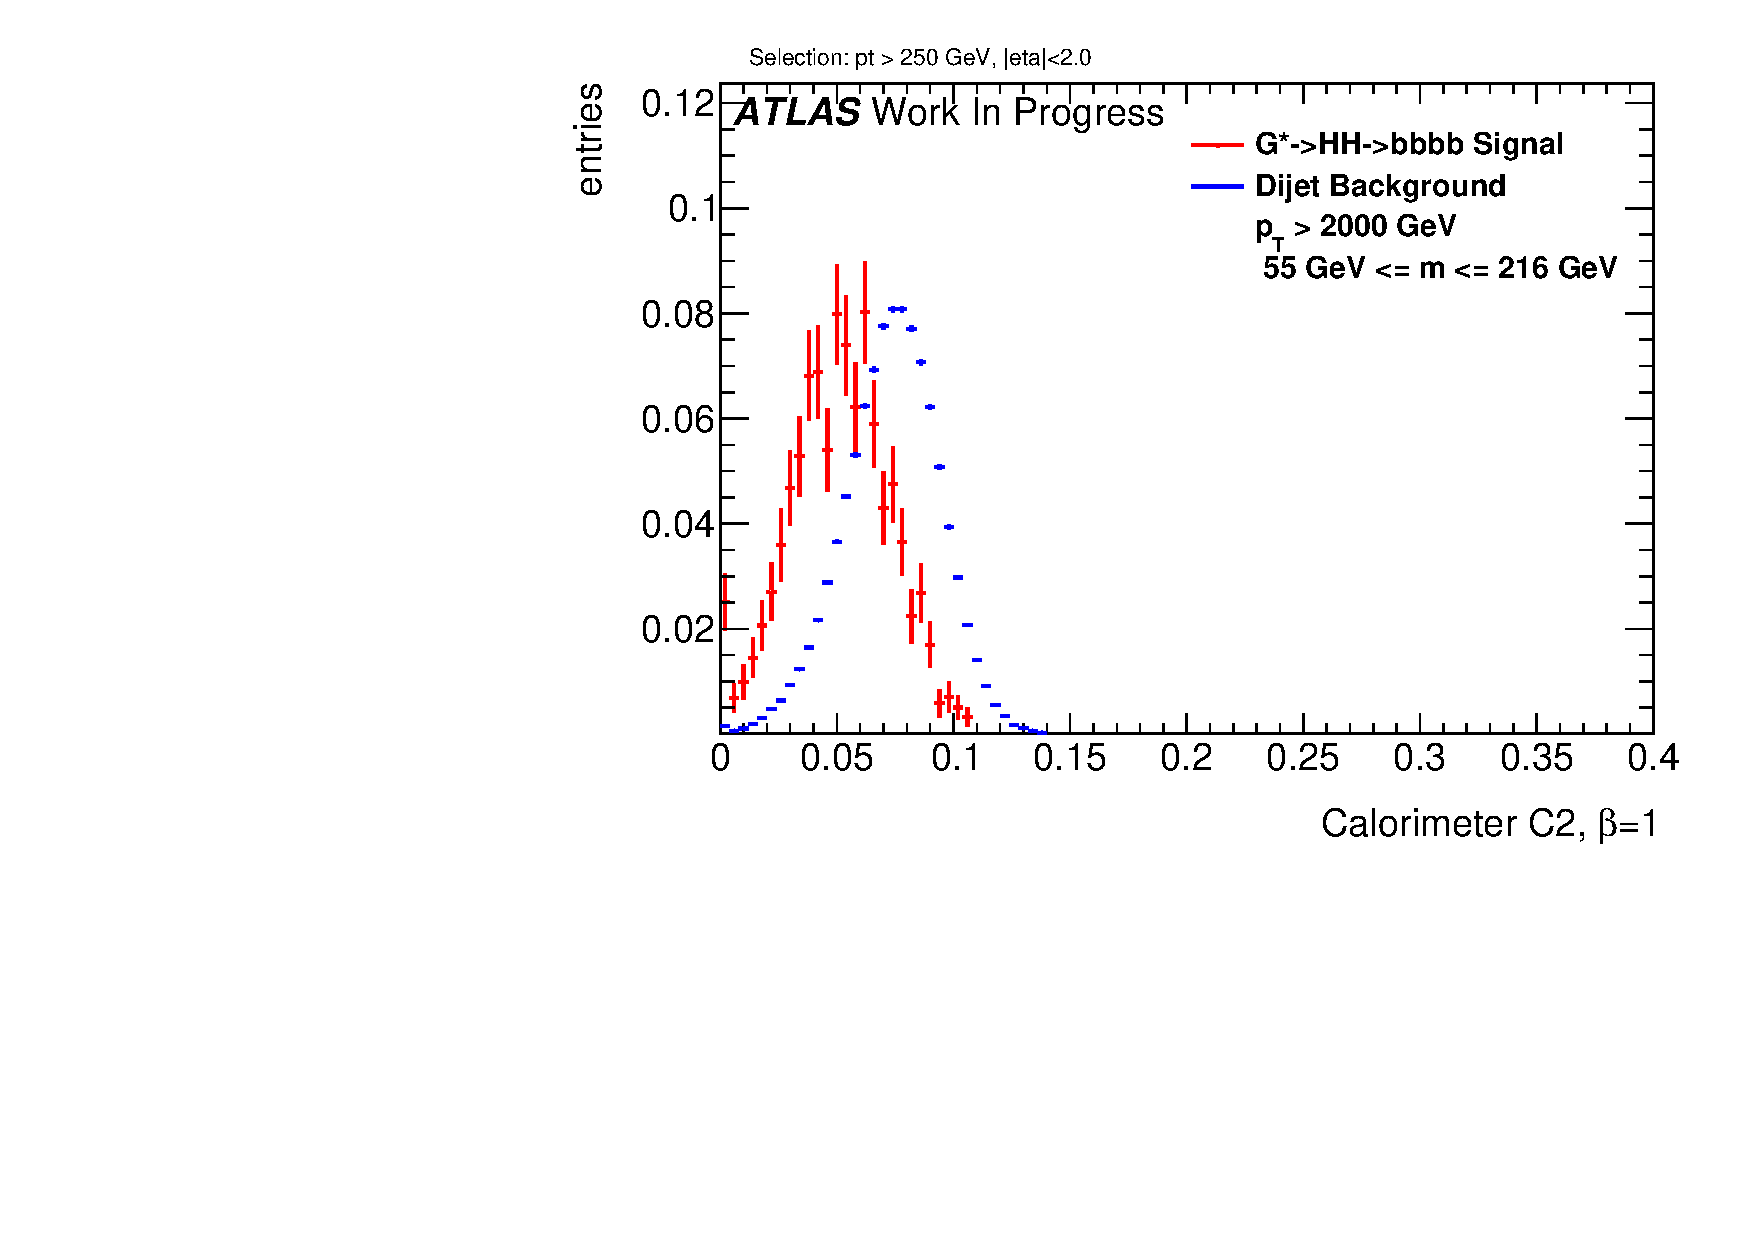
\includegraphics[width=0.3\textwidth]{sascha_input/plots/W/Beta1/h_recoJet_C2_bin6.pdf} 
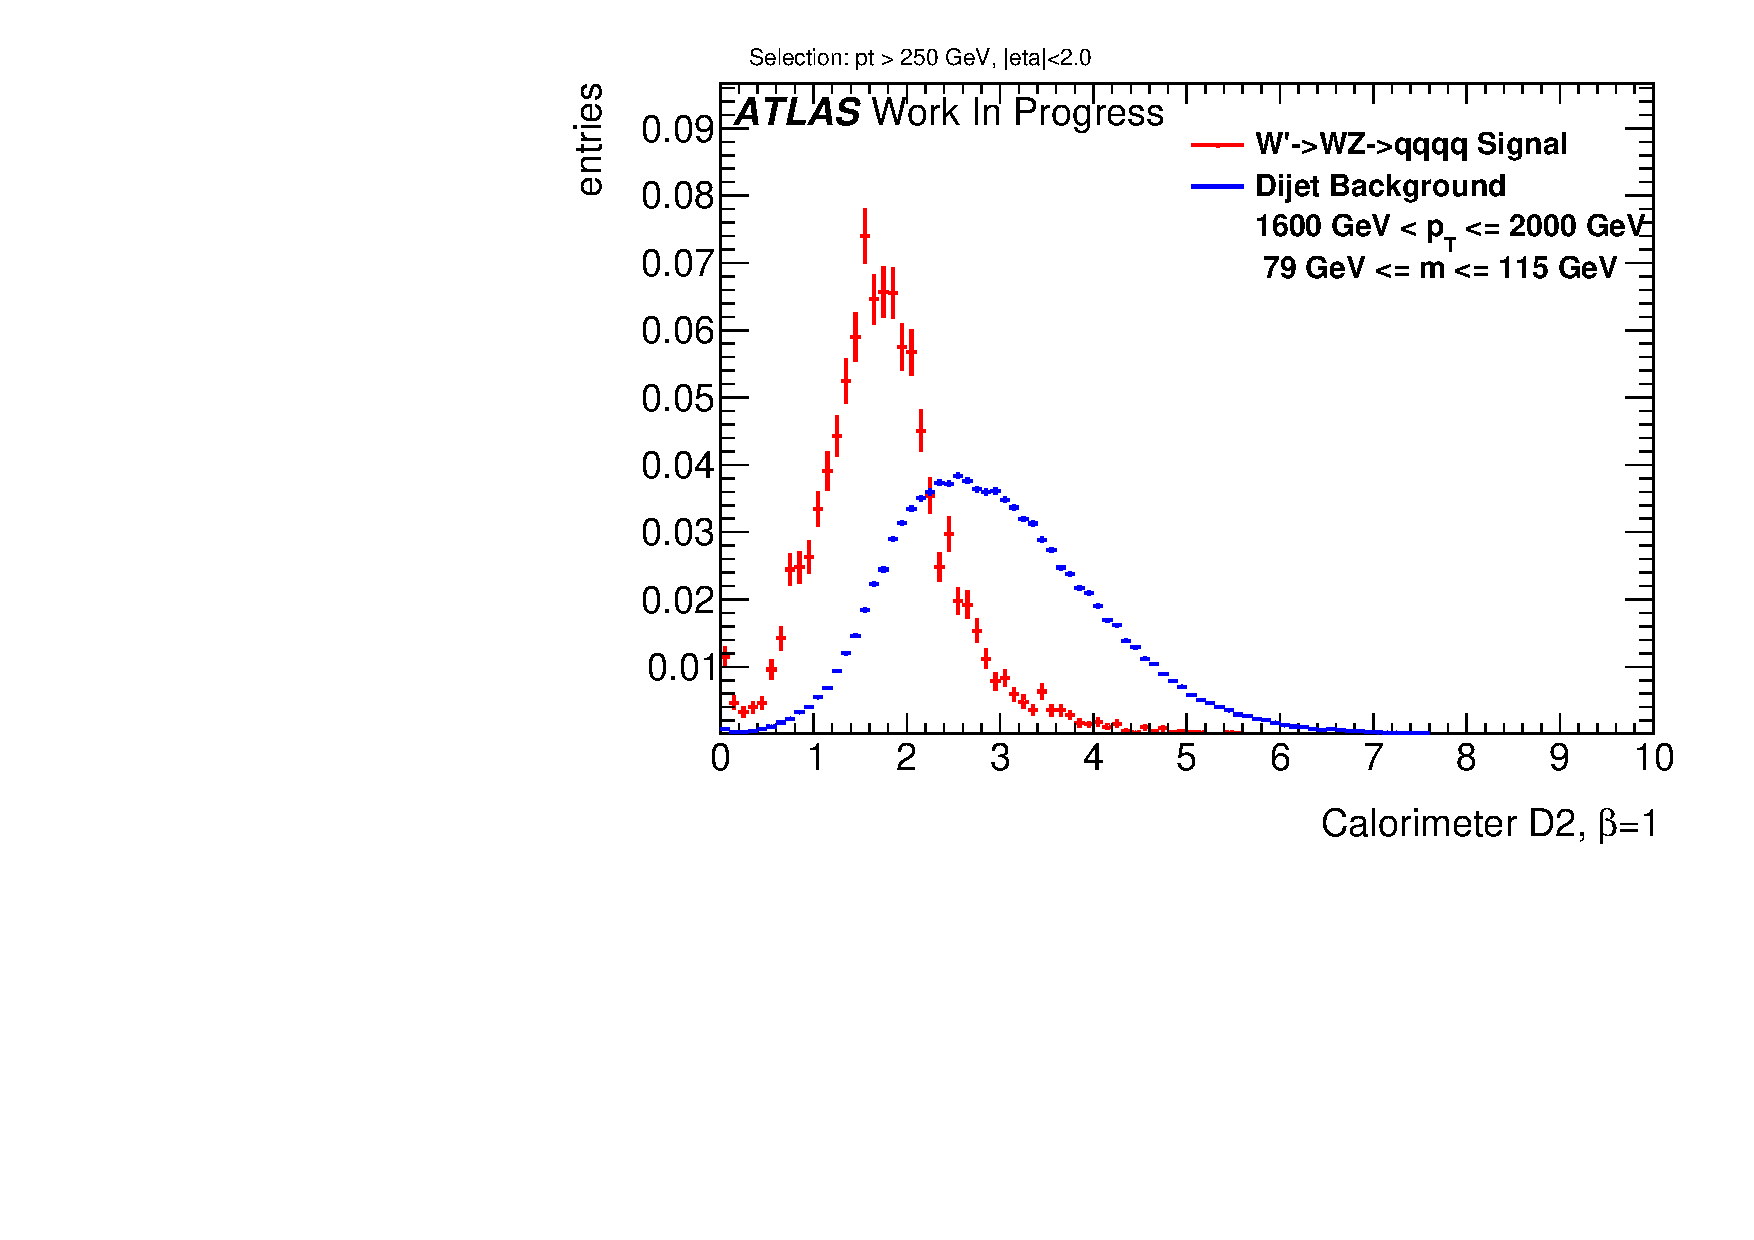
\includegraphics[width=0.3\textwidth]{sascha_input/plots/W/Beta1/h_recoJet_D2_bin5.pdf} 	
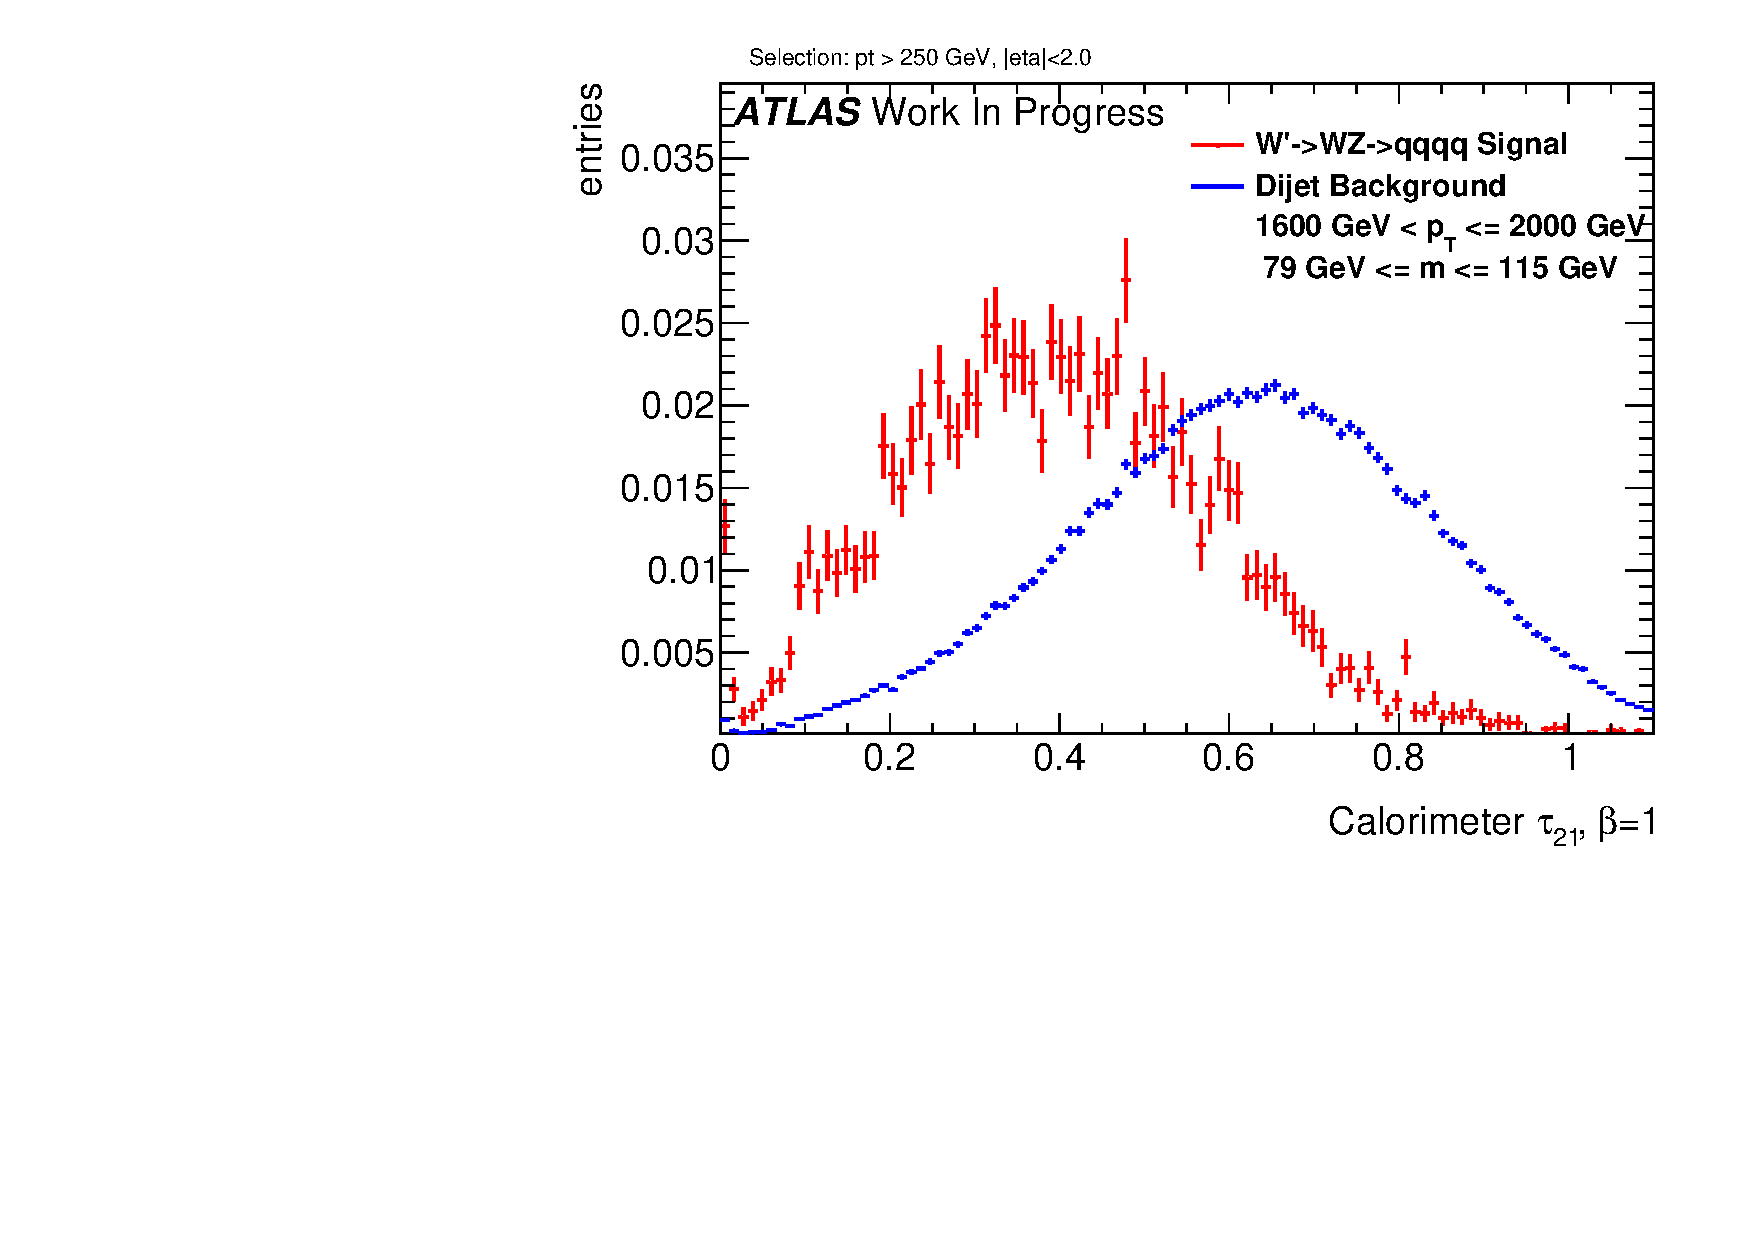
\includegraphics[width=0.3\textwidth]{sascha_input/plots/W/Beta1/h_recoJet_nSub21_bin5.pdf}
\bigskip
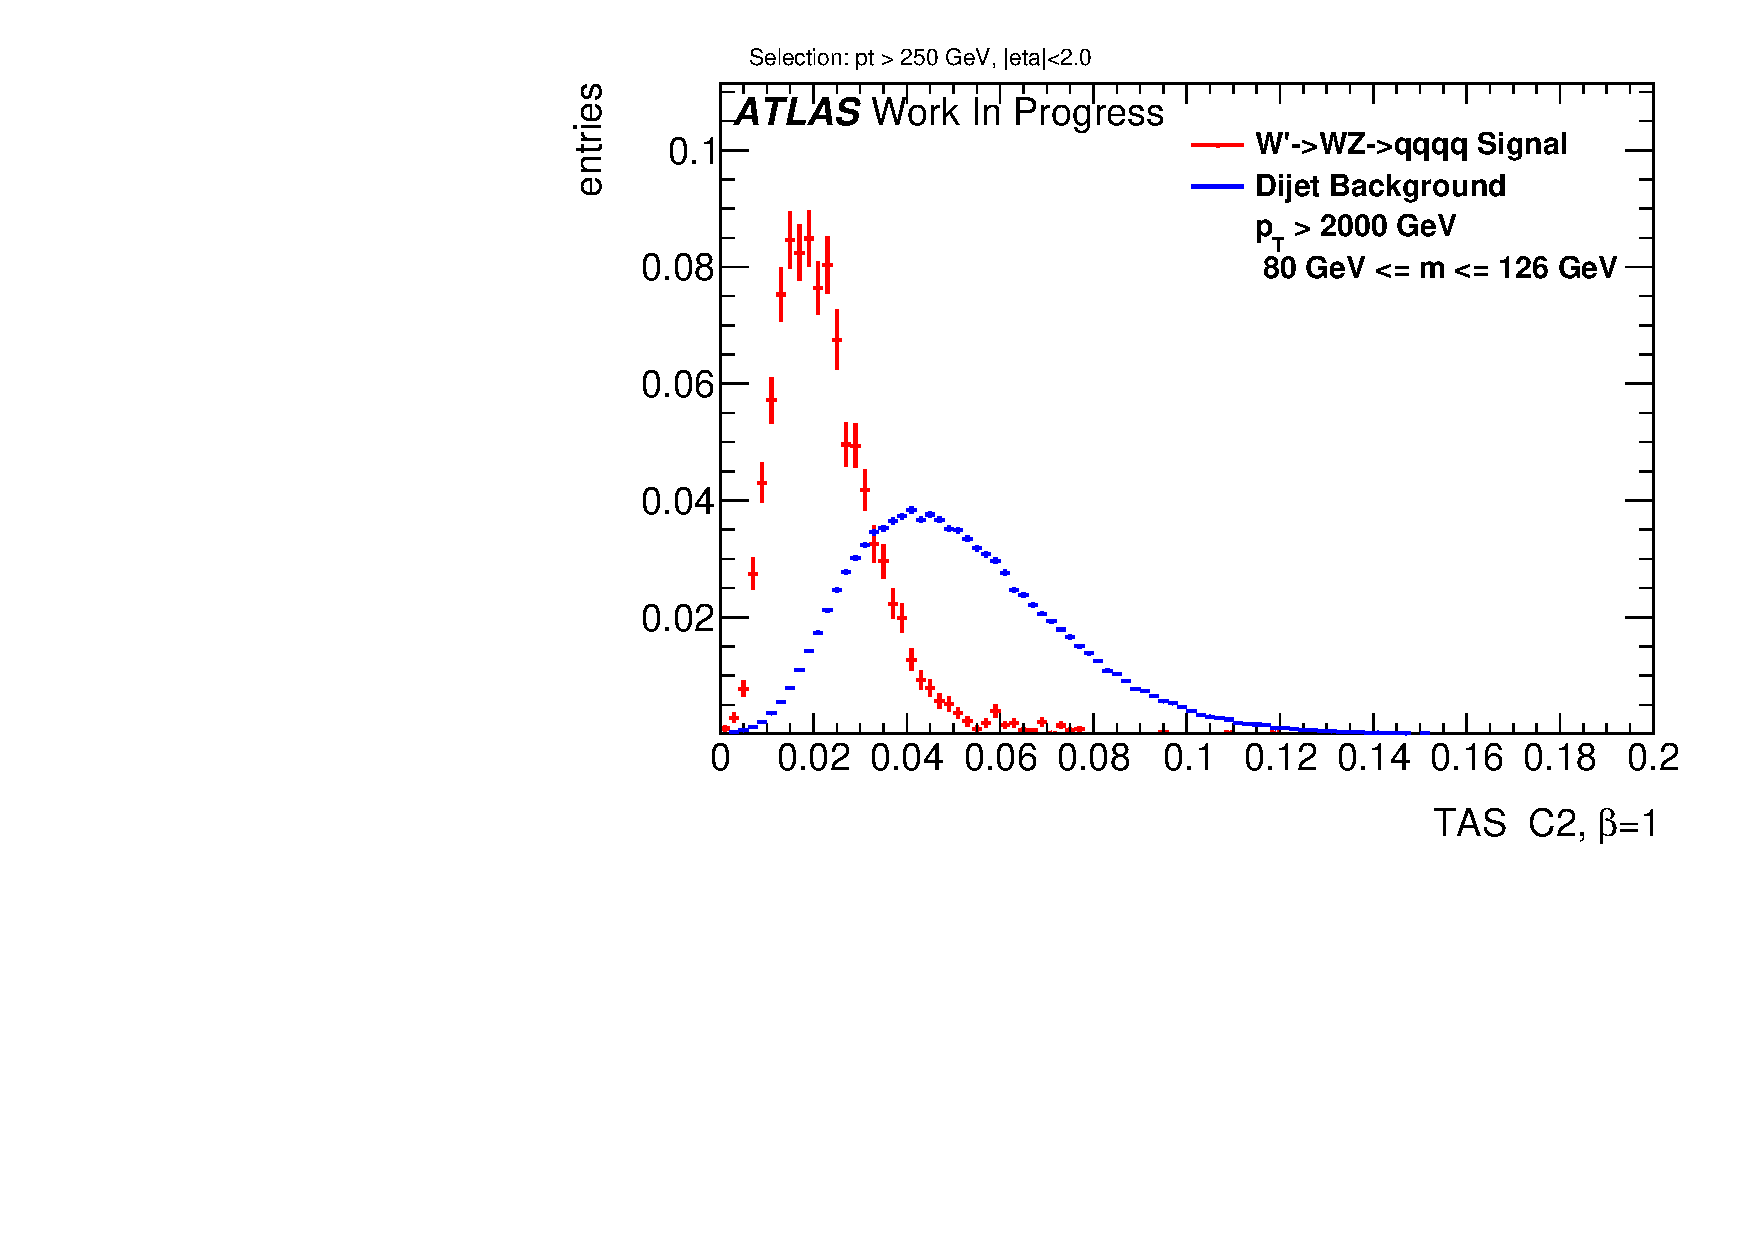
\includegraphics[width=0.3\textwidth]{sascha_input/plots/W/Beta1/h_assisted_tj_C2_bin6.pdf} \hspace{6mm}
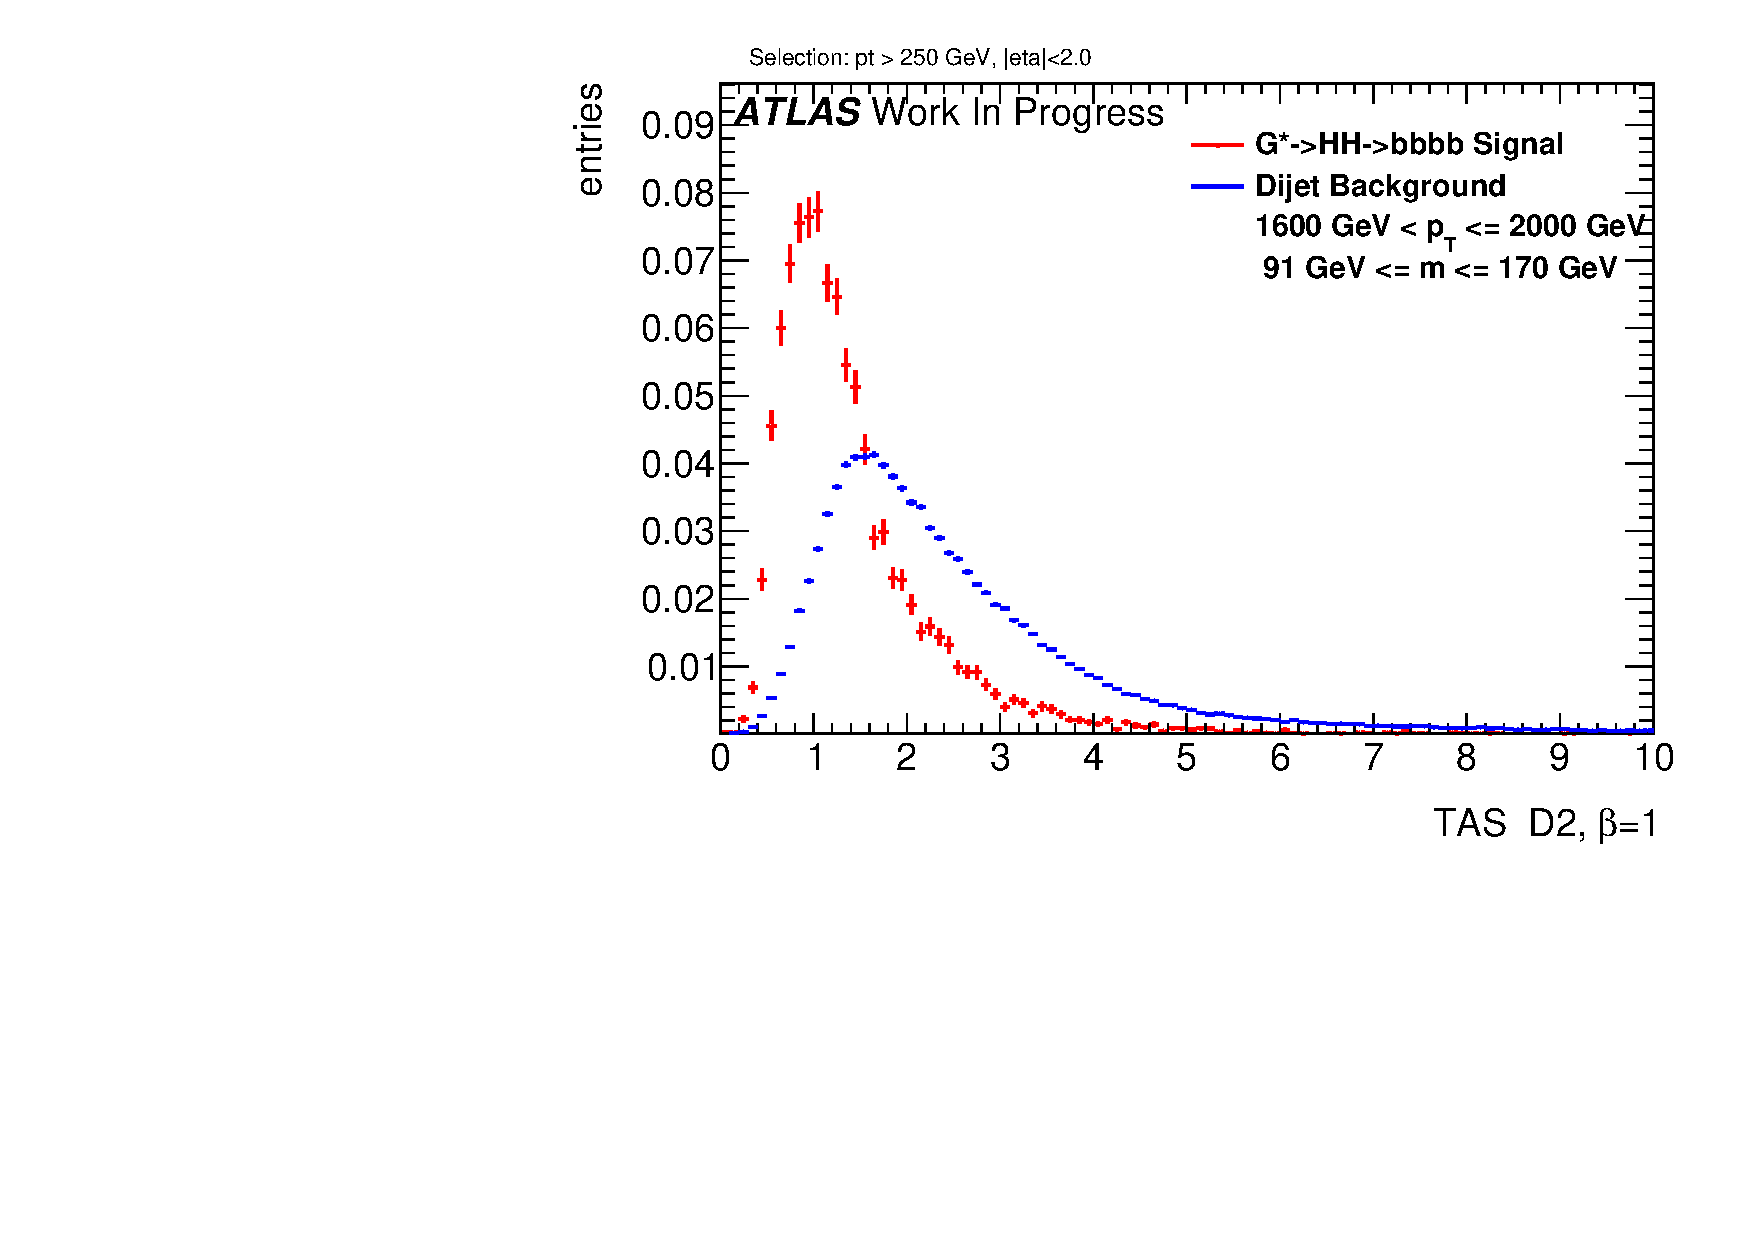
\includegraphics[width=0.3\textwidth]{sascha_input/plots/W/Beta1/h_assisted_tj_D2_bin5.pdf} \hspace{6mm}
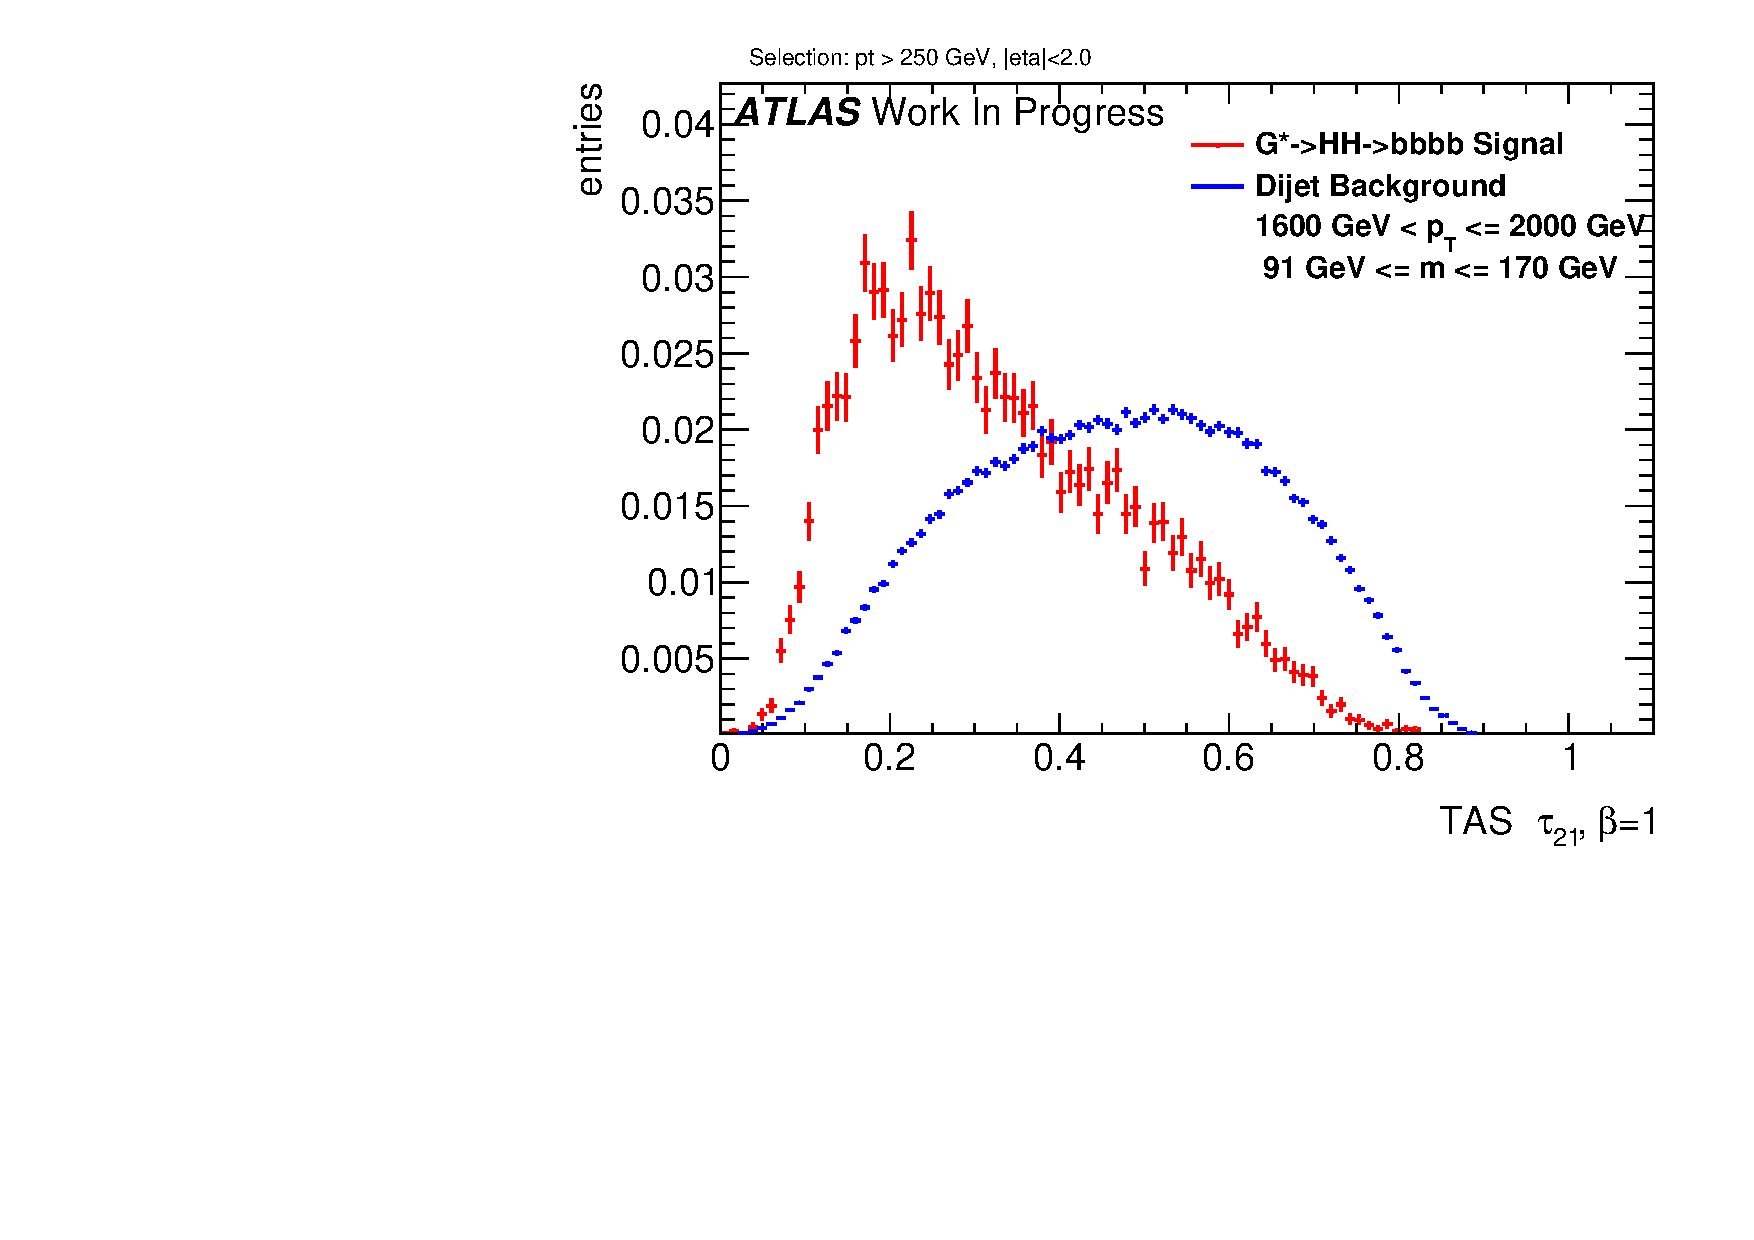
\includegraphics[width=0.3\textwidth]{sascha_input/plots/W/Beta1/h_assisted_tj_nSub21_bin5.pdf}
\caption{\footnotesize{$W$ boson signal and QCD background distributions for calorimeter (left) and TAS (right) at $\beta=1$  with C2 (top) for more than 2000 GeV and D2 (middle) and $\tau_{21}$ (bottom) for 1200-1600 GeV}}\label{fig:w_distribution_example}
\end{figure}

The ROCs in Figure \ref{fig:ROC_W_C2}, \ref{fig:ROC_W_D2} and \ref{fig:ROC_W_nSub21} show the actual achieved background rejection at different $p_T$ values. For lower $p_T$ values, TAS perform comparably to calorimeter clusters. Tracks without assisting achieve a considerably lower background rejection with D2 and $\tau_{21}$ for lower energies. Tracks and TAS perform equally well at high energies for D2 and $\tau_{21}$ and for C2 over the whole studied range. At higher boosts, the angular resolution of the tracks becomes more and more relevant as the separation between jet constituents shrinks. Consequently, tracks and TAS start to outperform calorimeter based variables and become increasingly effective with rising energy. 
\begin{figure}[htp]
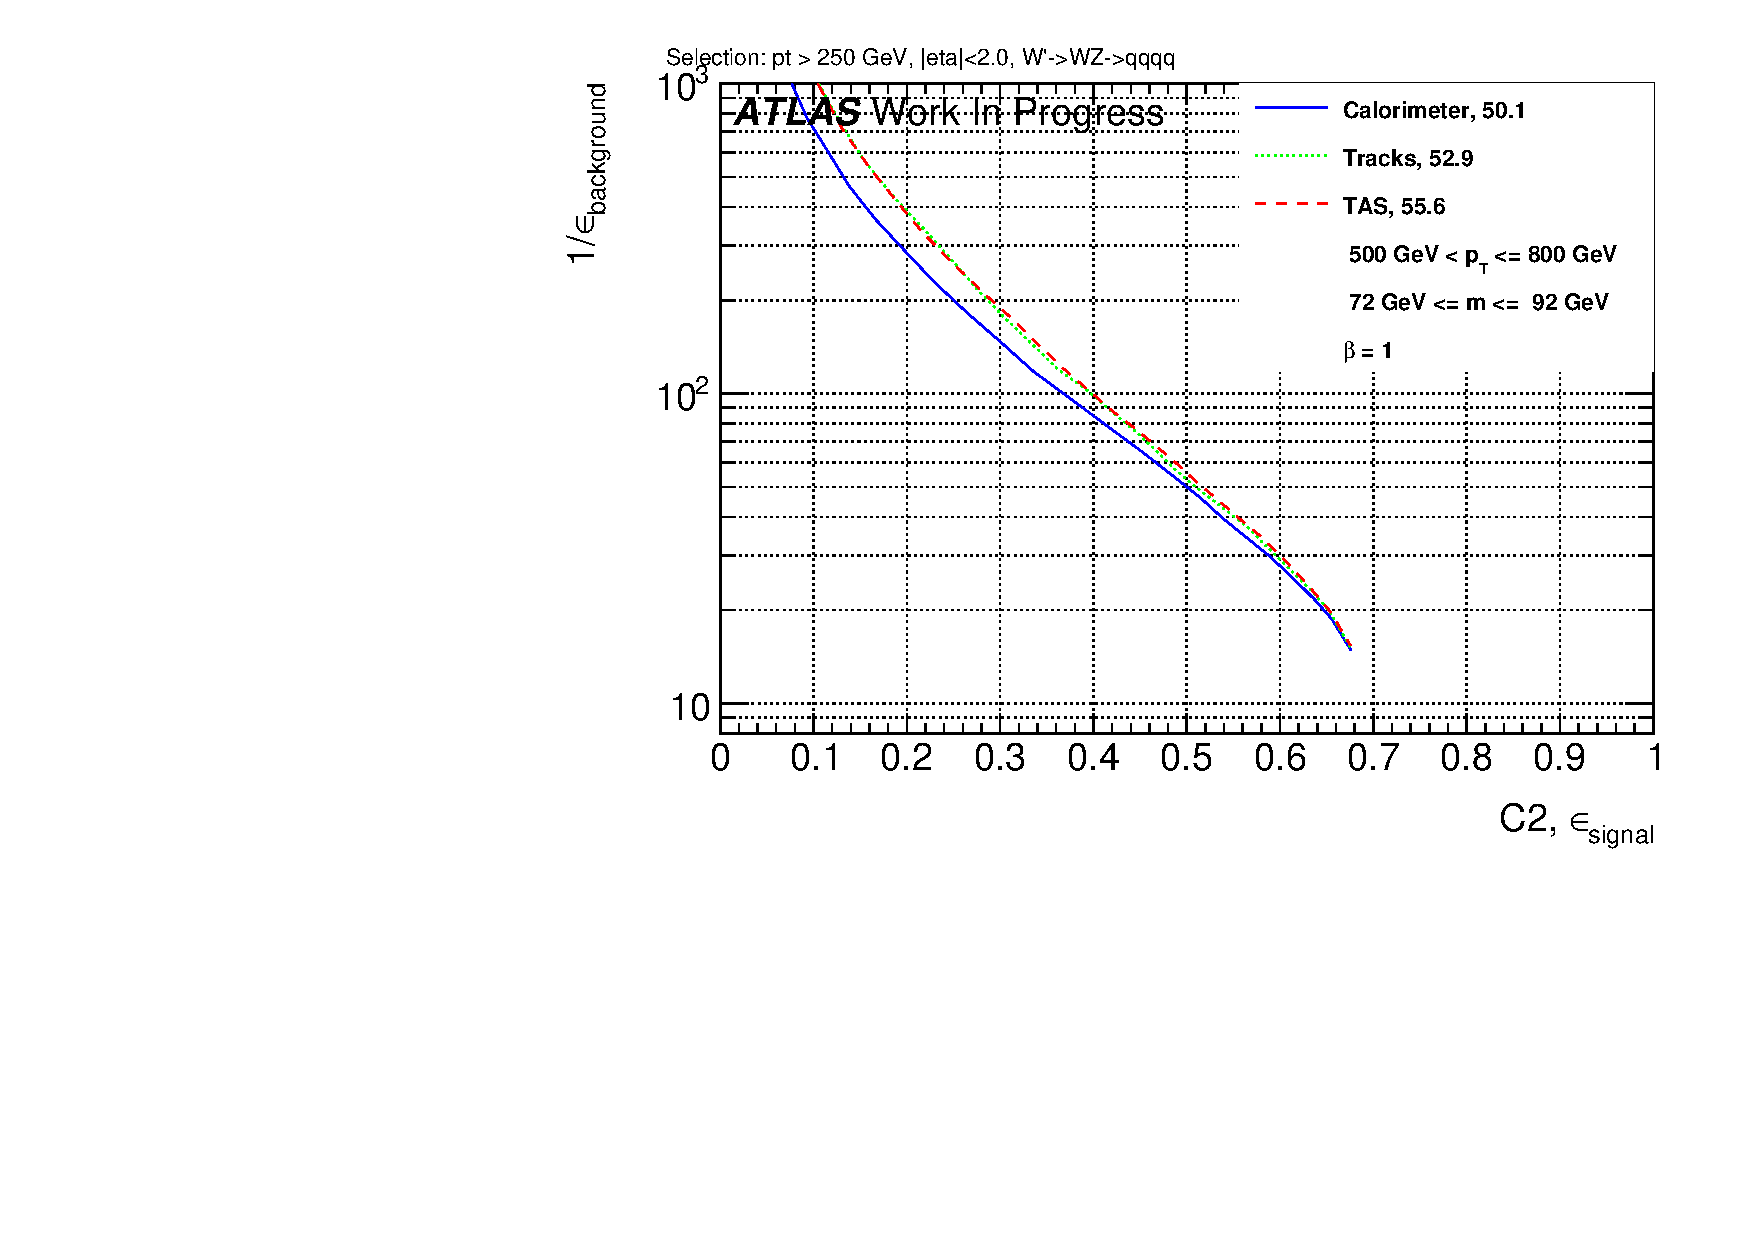
\includegraphics[width=0.5\textwidth]{sascha_input/plots/W/beta1/ROC_ALL_h_recoJet_C2_bin2.pdf} \hspace{1mm}
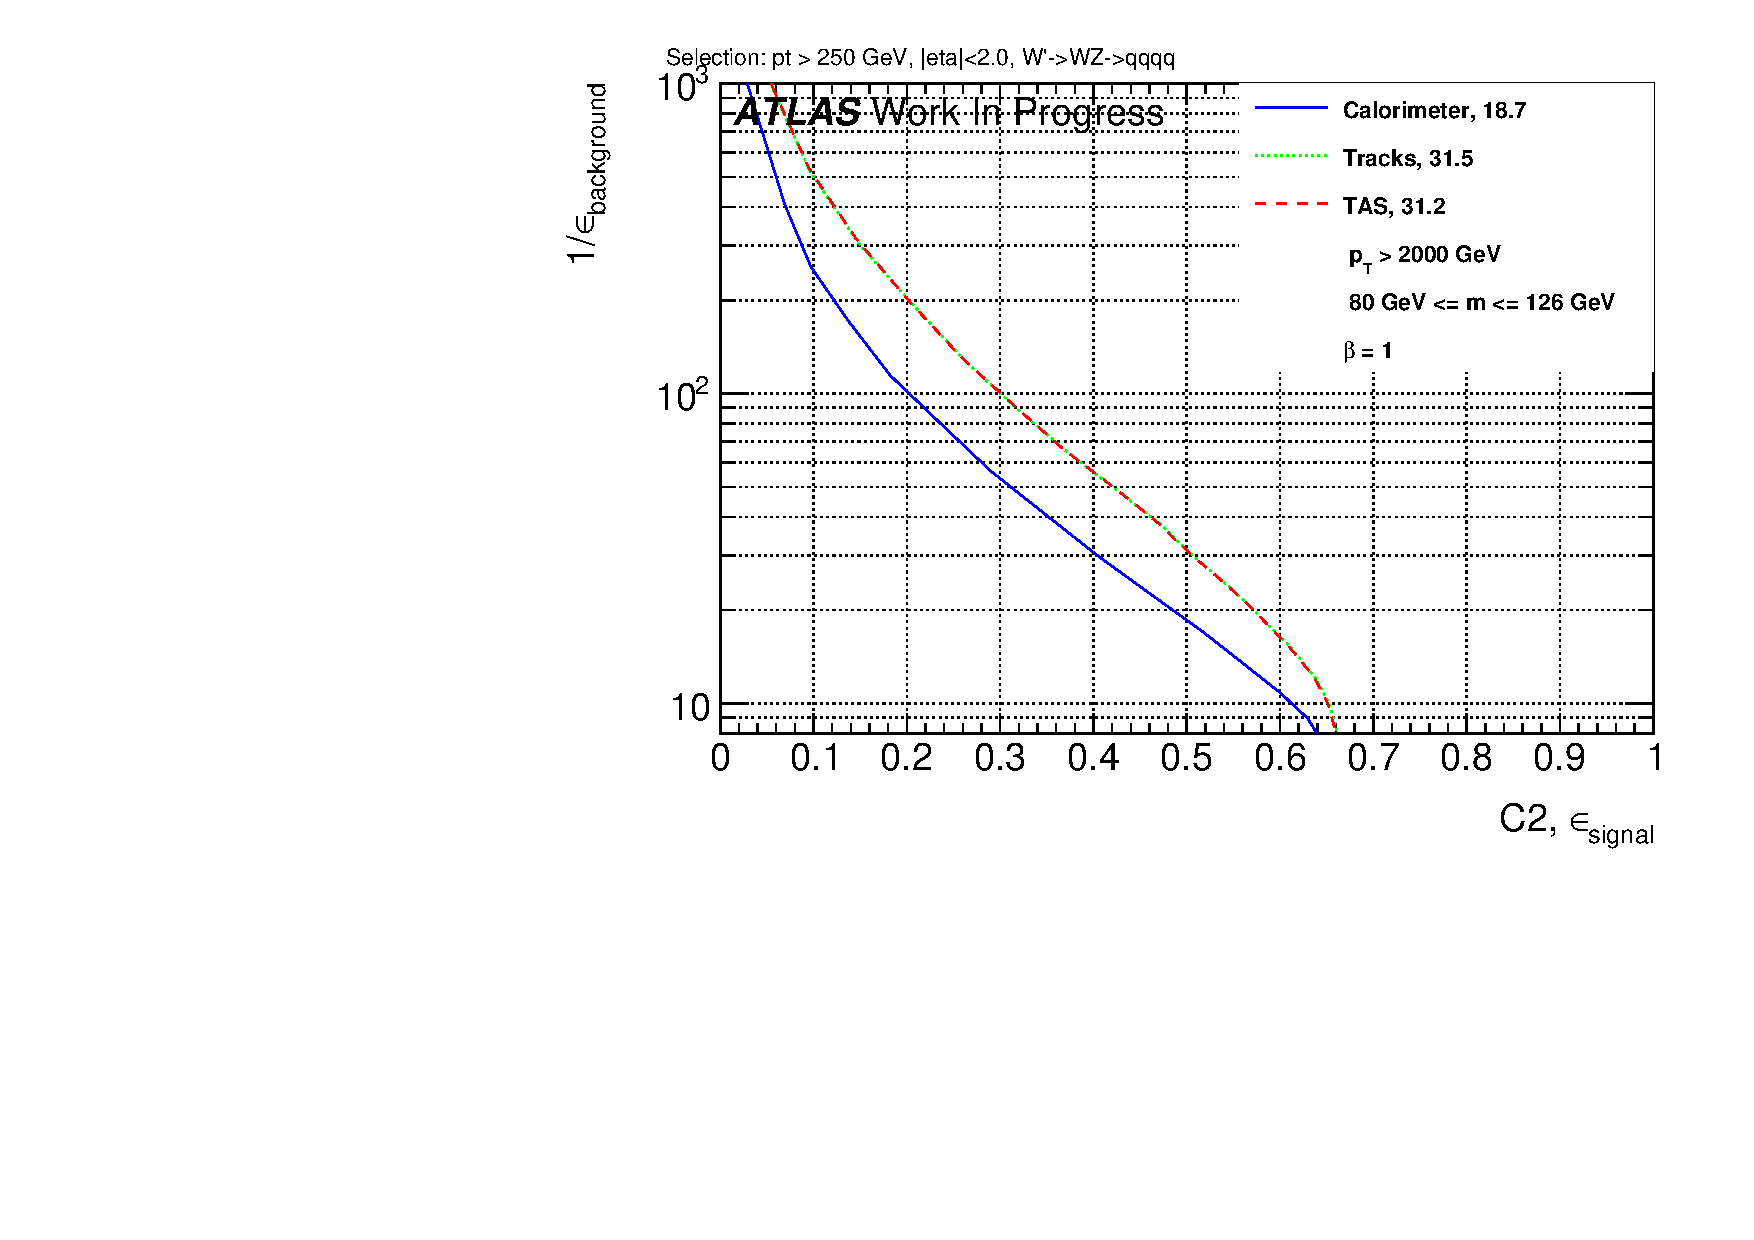
\includegraphics[width=0.5\textwidth]{sascha_input/plots/W/beta1/ROC_ALL_h_recoJet_C2_bin6.pdf}
\caption{\footnotesize{ROCs showing QCD rejection against $W$ boson efficiency for tracks, TAS and colorimeter C2 at $\beta=1$ for 500-800 GeV (left) and >2000 GeV (right). The numbers in the legend indicate the achieved background rejection at 50\% signal efficiency.}}\label{fig:ROC_W_C2}
\end{figure}

\begin{figure}[htp]
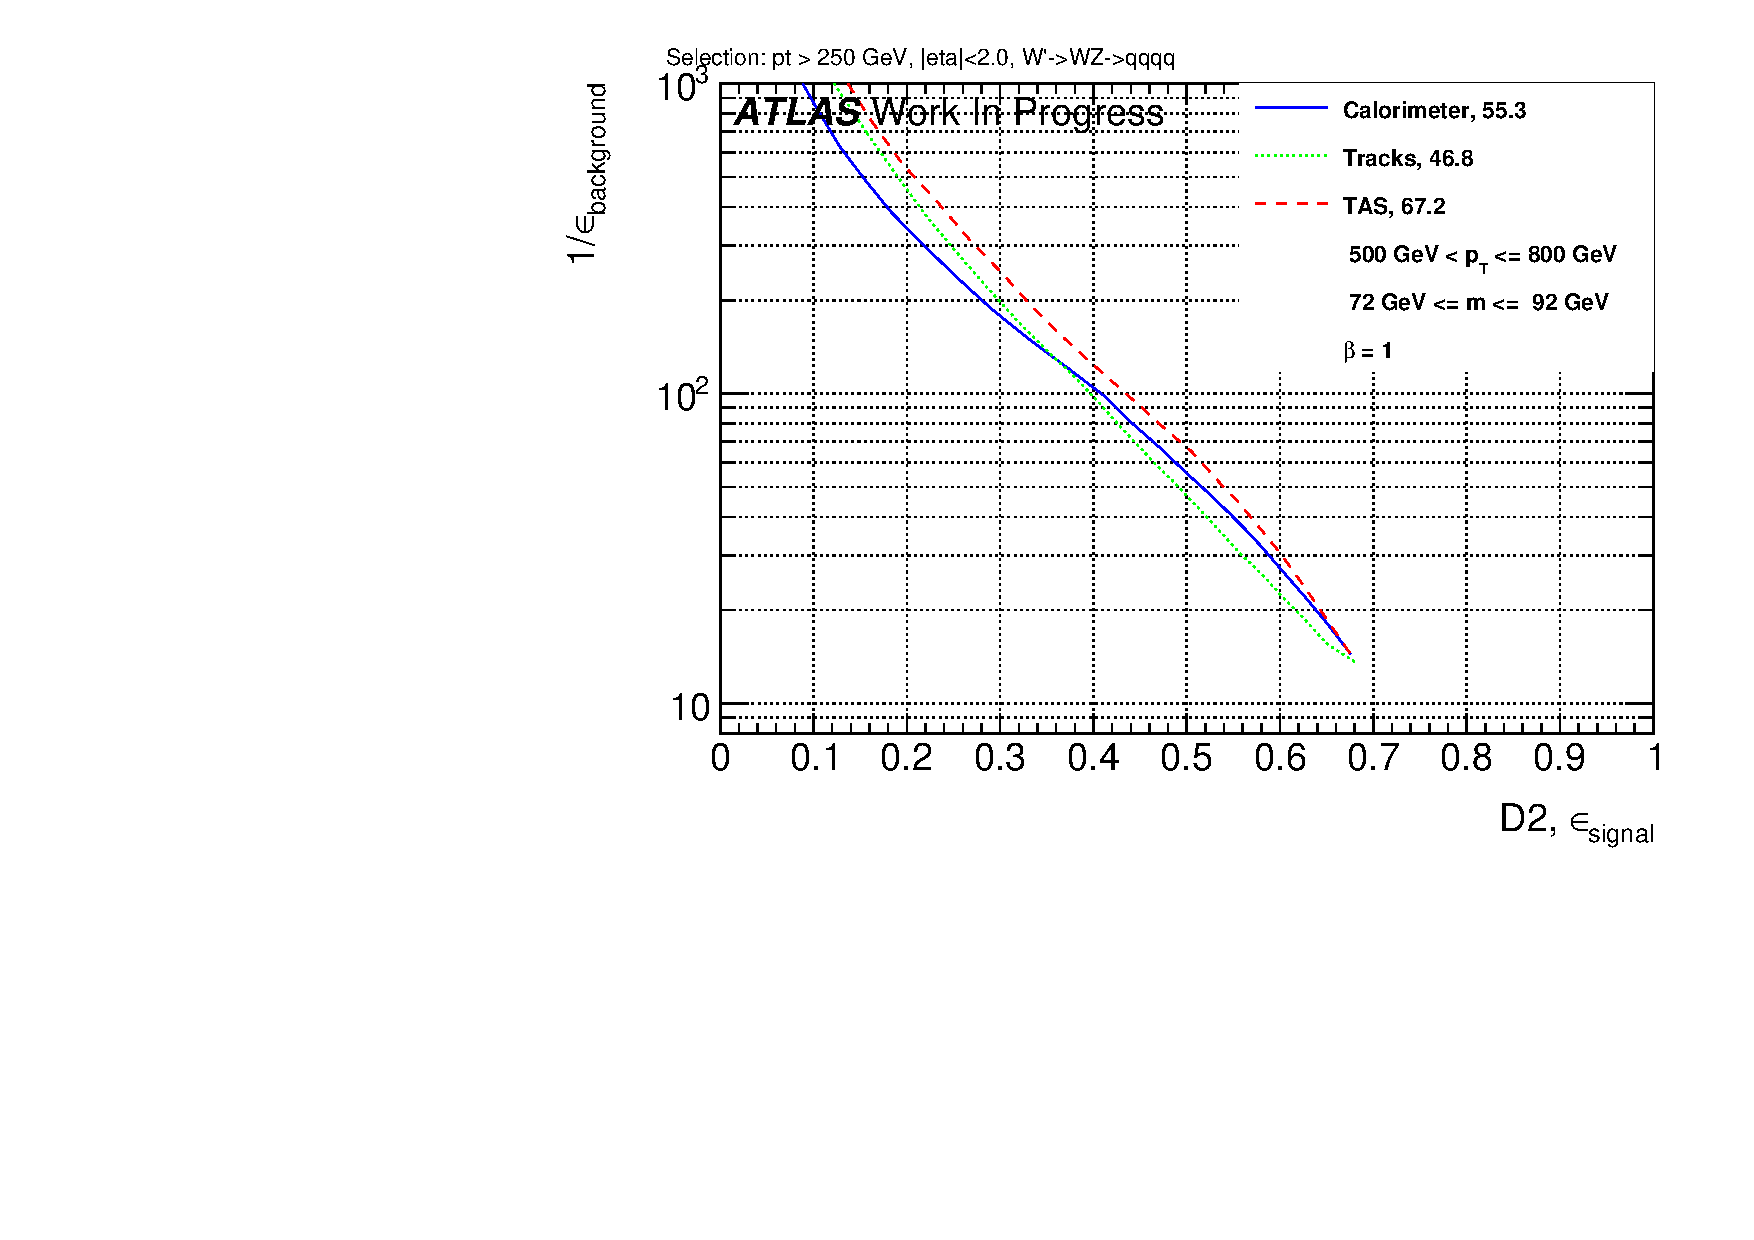
\includegraphics[width=0.5\textwidth]{sascha_input/plots/W/beta1/ROC_ALL_h_recoJet_D2_bin2.pdf}
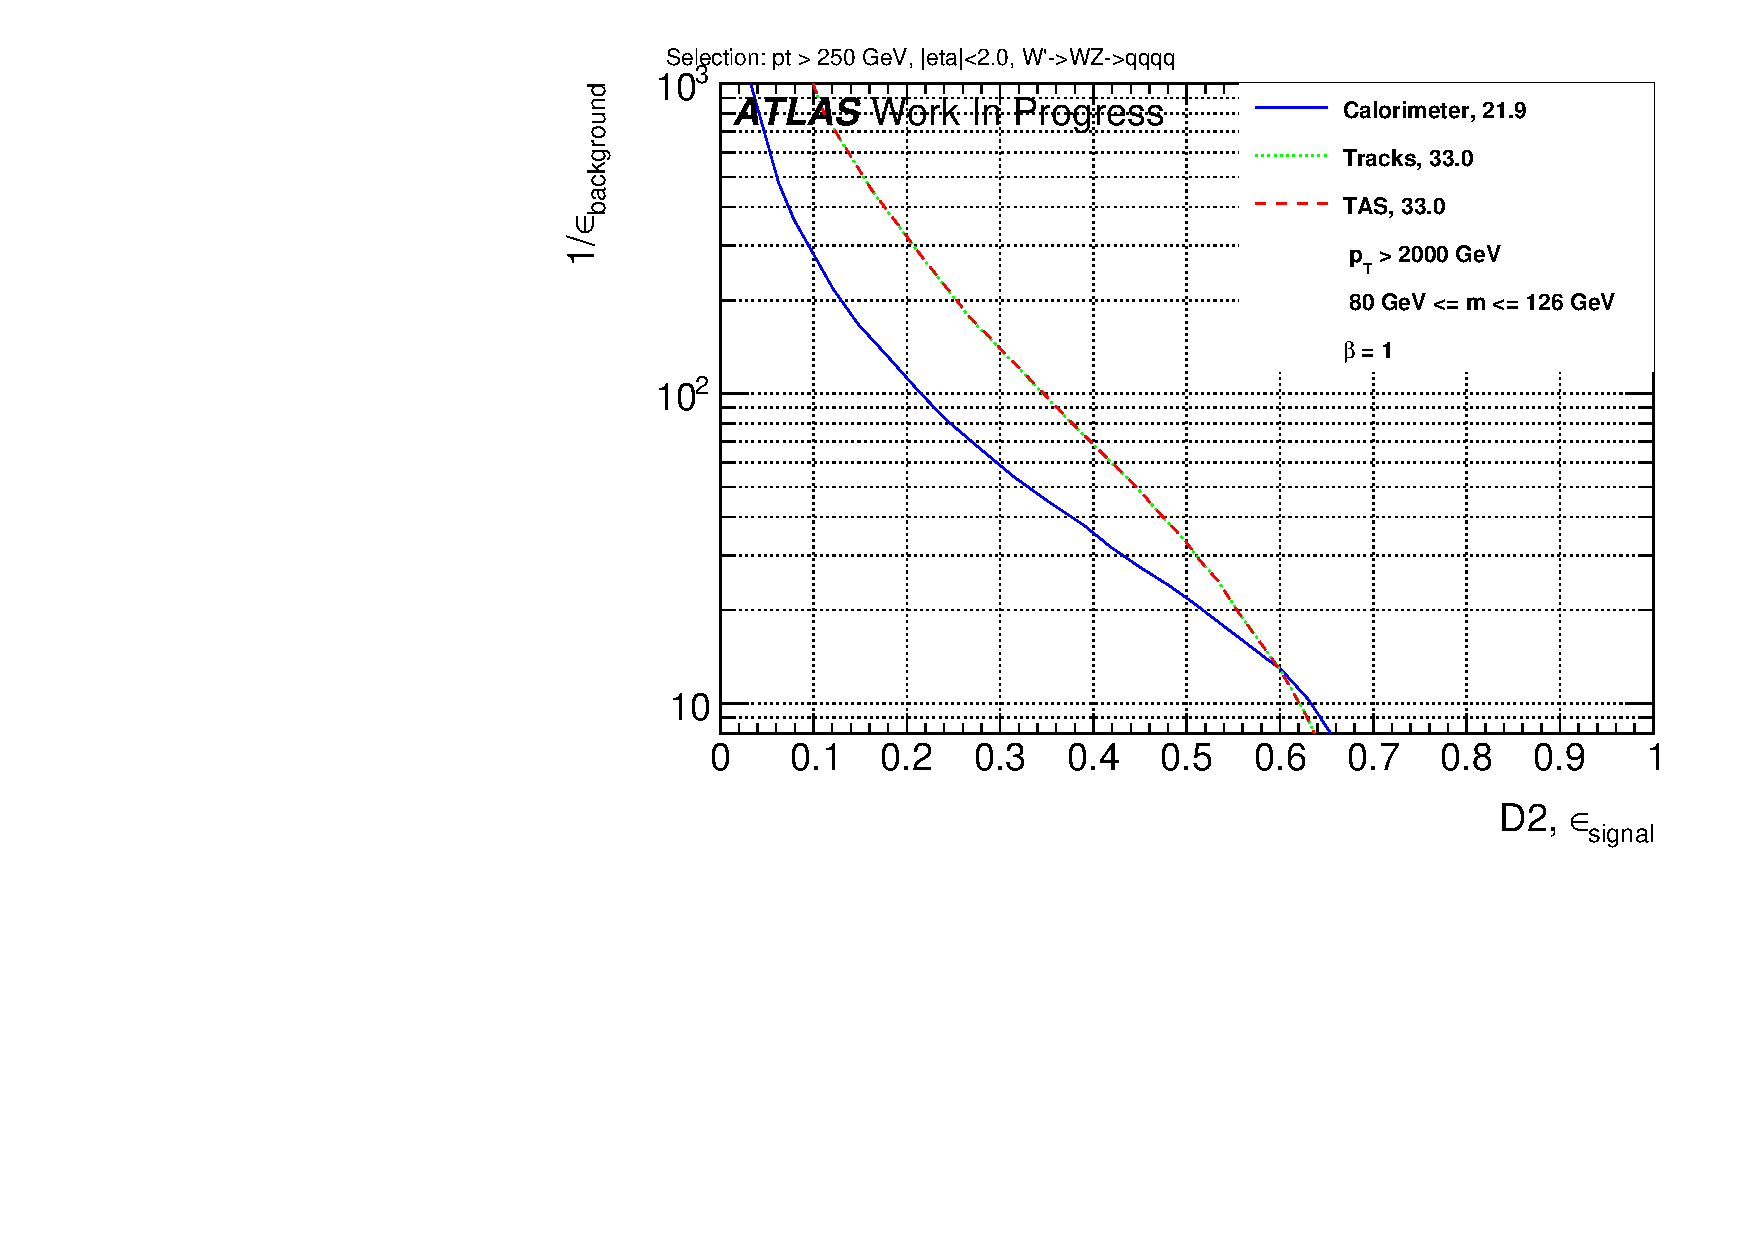
\includegraphics[width=0.5\textwidth]{sascha_input/plots/W/beta1/ROC_ALL_h_recoJet_D2_bin6.pdf}
\caption{\footnotesize{ROCs showing QCD rejection against $W$ boson efficiency for tracks, TAS and colorimeter D2 at $\beta=1$ for 500-800 GeV (left) and >2000 GeV (right). The numbers in the legend indicate the achieved background rejection at 50\% signal efficiency.}}\label{fig:ROC_W_D2}
\end{figure}

\begin{figure}[htp]
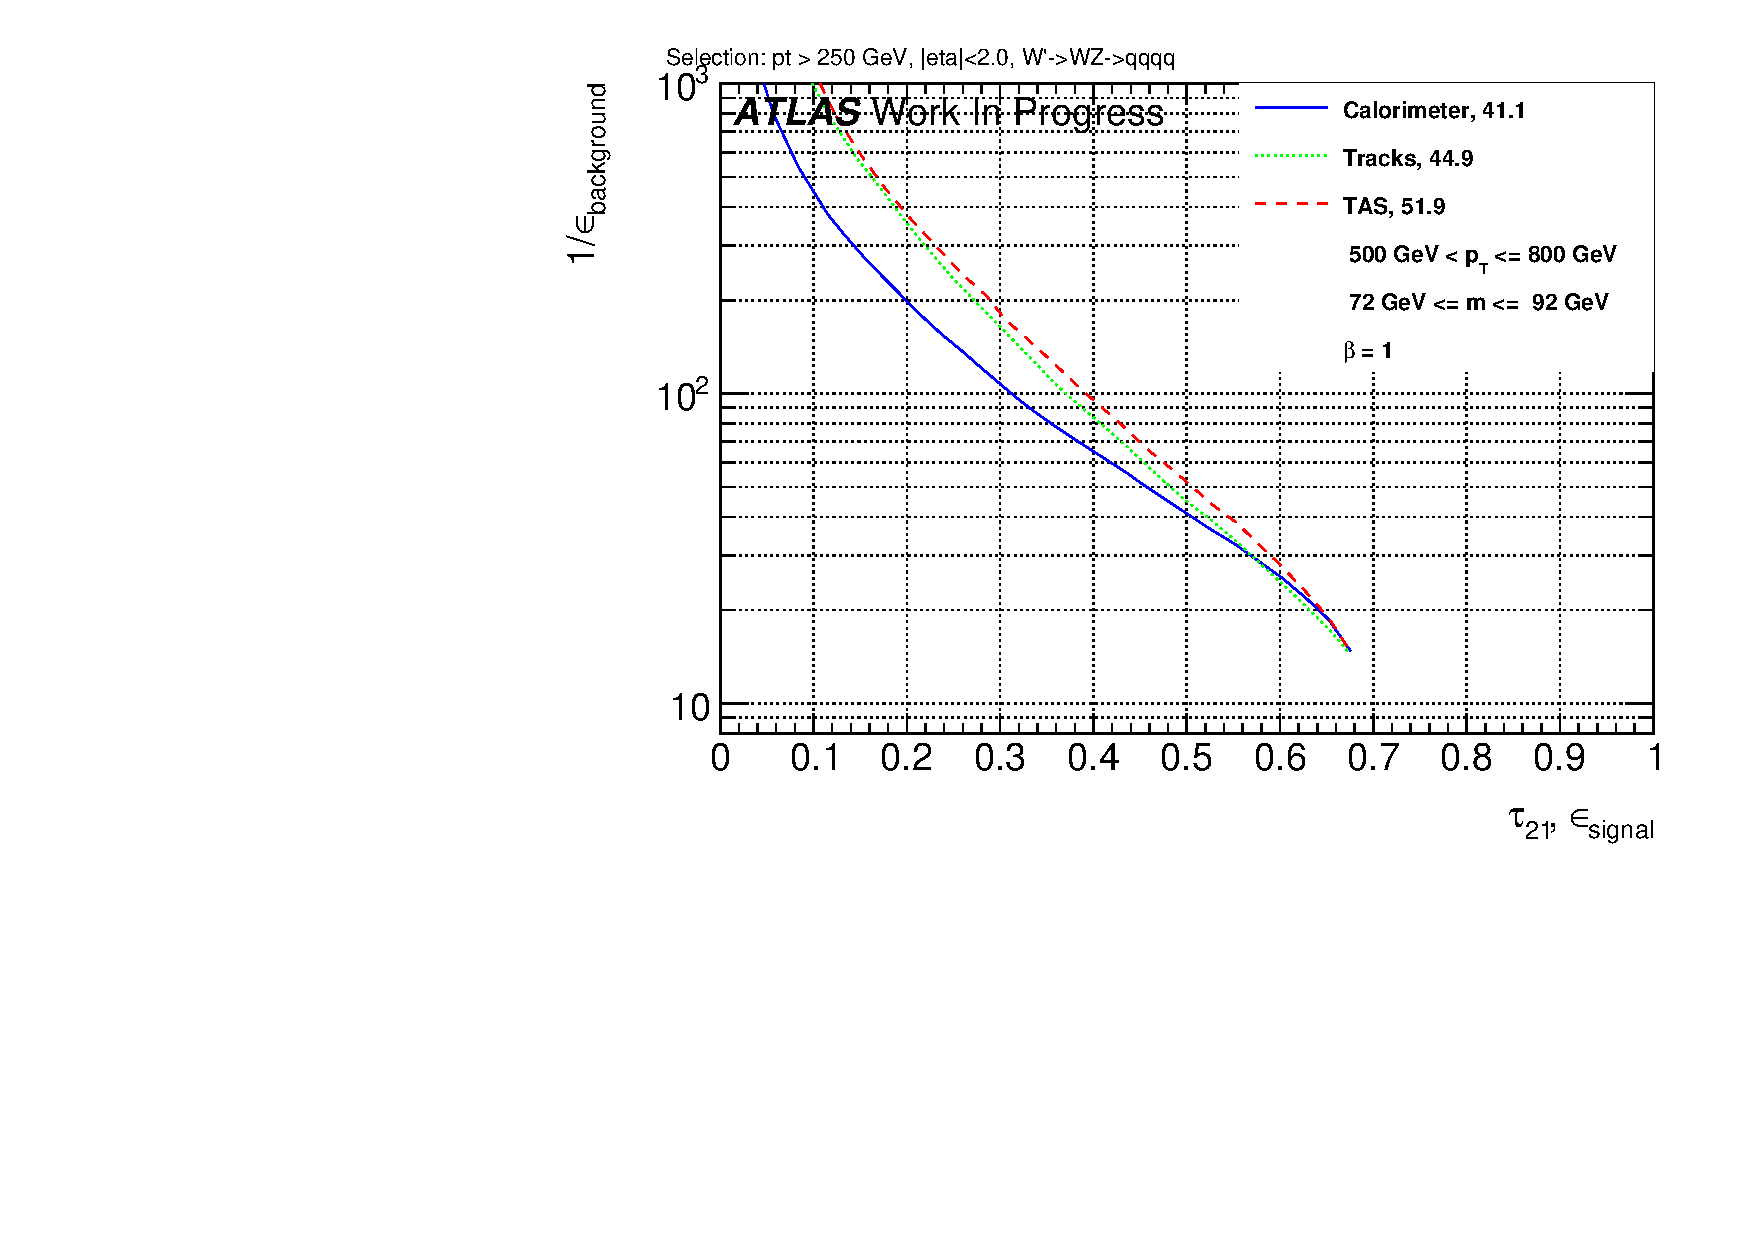
\includegraphics[width=0.5\textwidth]{sascha_input/plots/W/beta1/ROC_ALL_h_recoJet_nSub21_bin2.pdf}
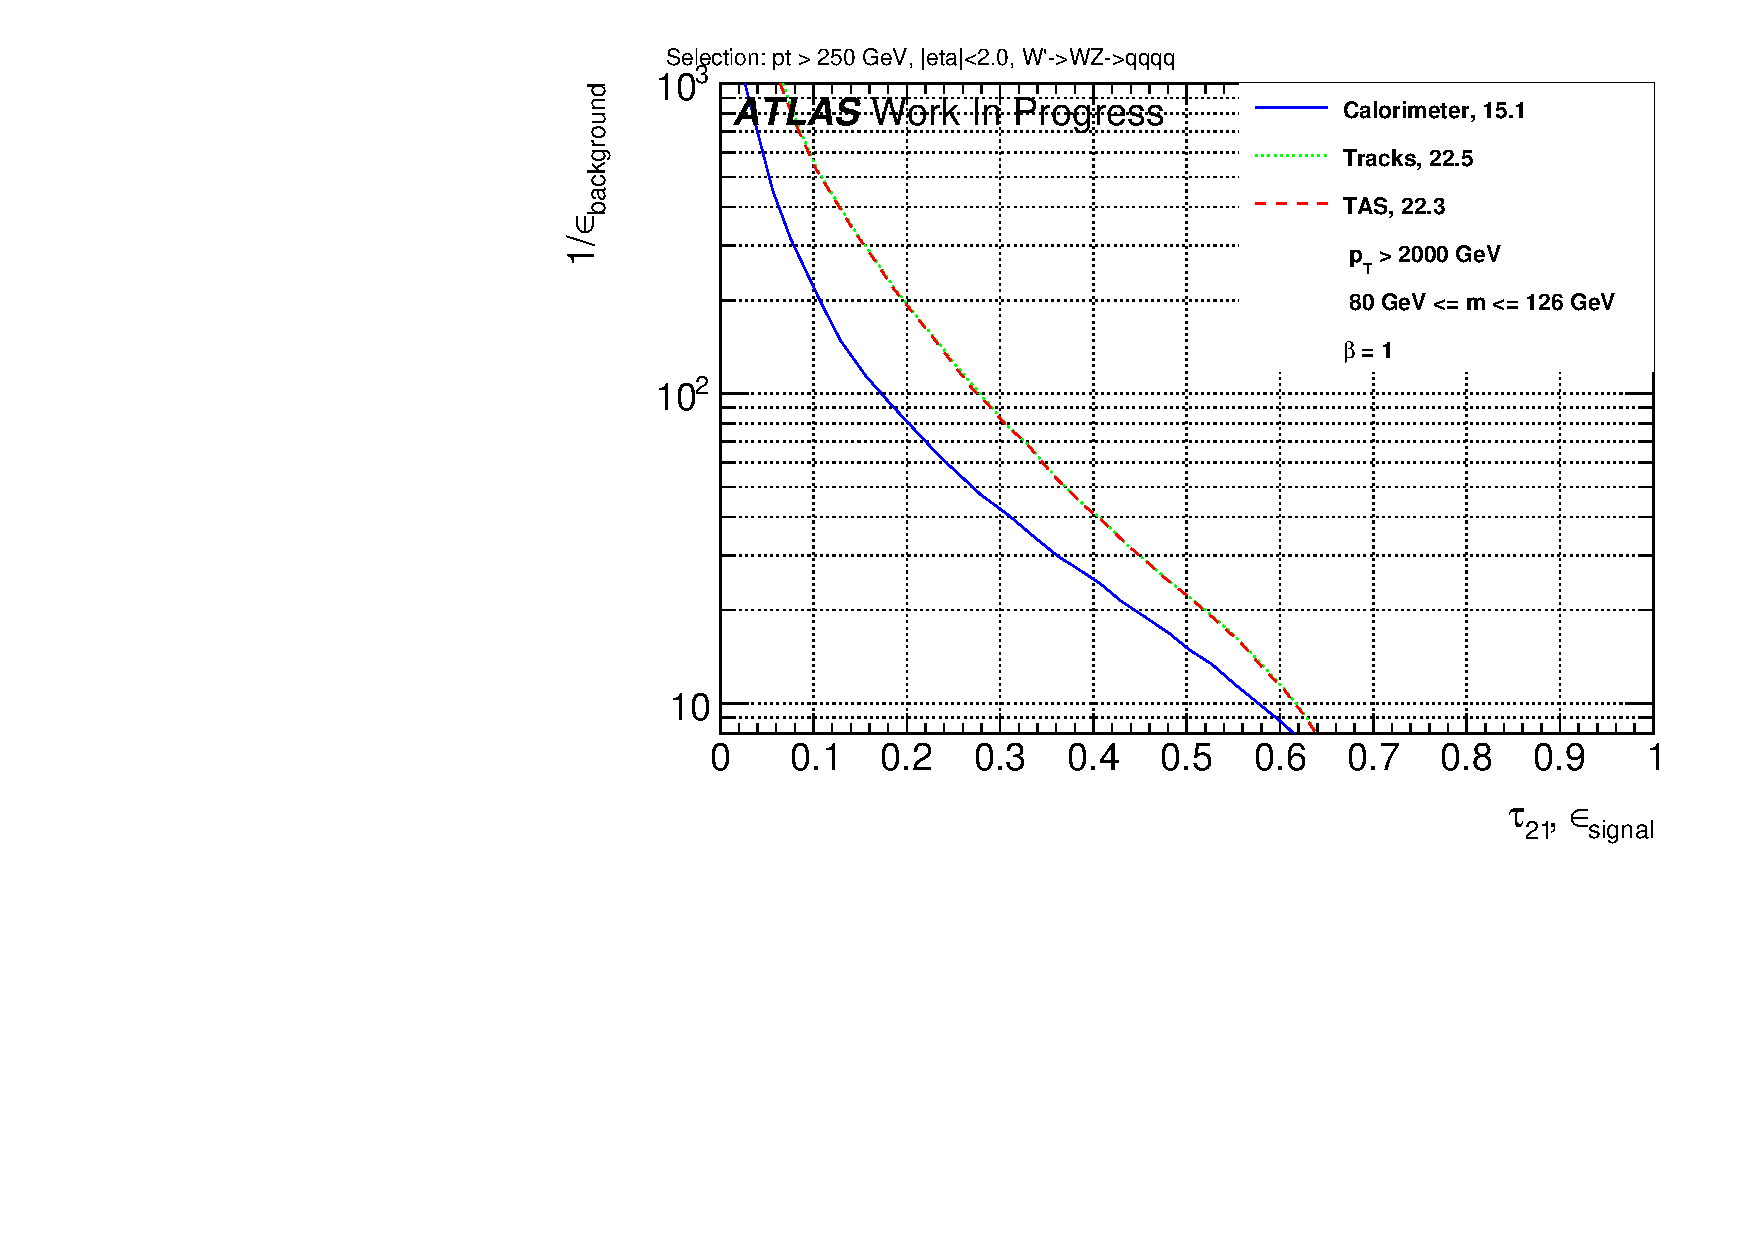
\includegraphics[width=0.5\textwidth]{sascha_input/plots/W/beta1/ROC_ALL_h_recoJet_nSub21_bin6.pdf}
\caption{\footnotesize{ROCs showing QCD rejection against $W$ boson efficiency for tracks, TAS and colorimeter $\tau_{21}$ at $\beta=1$ for 500-800 GeV (left) and >2000 GeV (right). The numbers in the legend indicate the achieved background rejection at 50\% signal efficiency.}}\label{fig:ROC_W_nSub21}
\end{figure}

\subsubsection{Un-assisted tracks and TAS at very high $p_{\mathrm{T}}$}
The C2 variable was found to perform equally well with tracks and TAS as input. This variable seems to be relative insensitive to the track assisting and tracks alone already perform well. D2 and $\tau_{21}$ in contrast, feature a visibly worse separation with tracks than with assisted tracks. In these cases, the scale difference due to the missing neutral fraction seems to have a greater influence.

For very high $p_{\mathrm{T}}$ values however, it is often the case that the large-R calorimeter jet features only one $R = 0.2$ sub-jet after trimming due to the now small separation of constituents. A single sub-jet results in the TAS procedure to fall back to TA. As stated in Section \ref{subsec:ta_adapt}, TA has no impact on the ratios. Therefore, C2/D2 and $\tau_{21}$ perform equally well when calculated with tracks or TAS for events with only one sub-jet and thereby the difference between both decreases for very high energies. 


\subsubsection{Correlation with $p_{\mathrm{T}}$}
Due to the rapidly falling $p_{\mathrm{T}}$ spectrum and hence low weights for high $p_{\mathrm{T}}$ are the correlation plots divided into the six different $p_{\mathrm{T}}$ regions.
For C2, see Figure \ref{fig:correlation_C2}, one can observe a strong trend to lower values for signal and background with calorimeter clusters as well as TAS. Furthermore, it is possible to observe that the TAS distributions concentrate at lower values compared to calorimeter counterparts.

In the cases of D2, Figure \ref{fig:correlation_D2}, and $\tau_{21}$, Figure \ref{fig:correlation_tau21}, there is a small upward trend of the calorimeter variables visible in the lower $p_{\mathrm{T}}$ regions which, with rising boost, slows down for D2 and $\tau_{21}$ and ends for $\tau_{21}$ in a broader distribution. This verifies the higher $p_{\mathrm{T}}$ dependence of the C2 variable in comparison to D2 and $\tau_{21}$. The TAS counterparts feature an even more robust signal with the background moving to higher values, hence improving separation. The $p_{\mathrm{T}}$ dependence of variables calculated with tracks is very similar to the ones with TAS, therefore they are omitted.

\begin{figure}[htp]
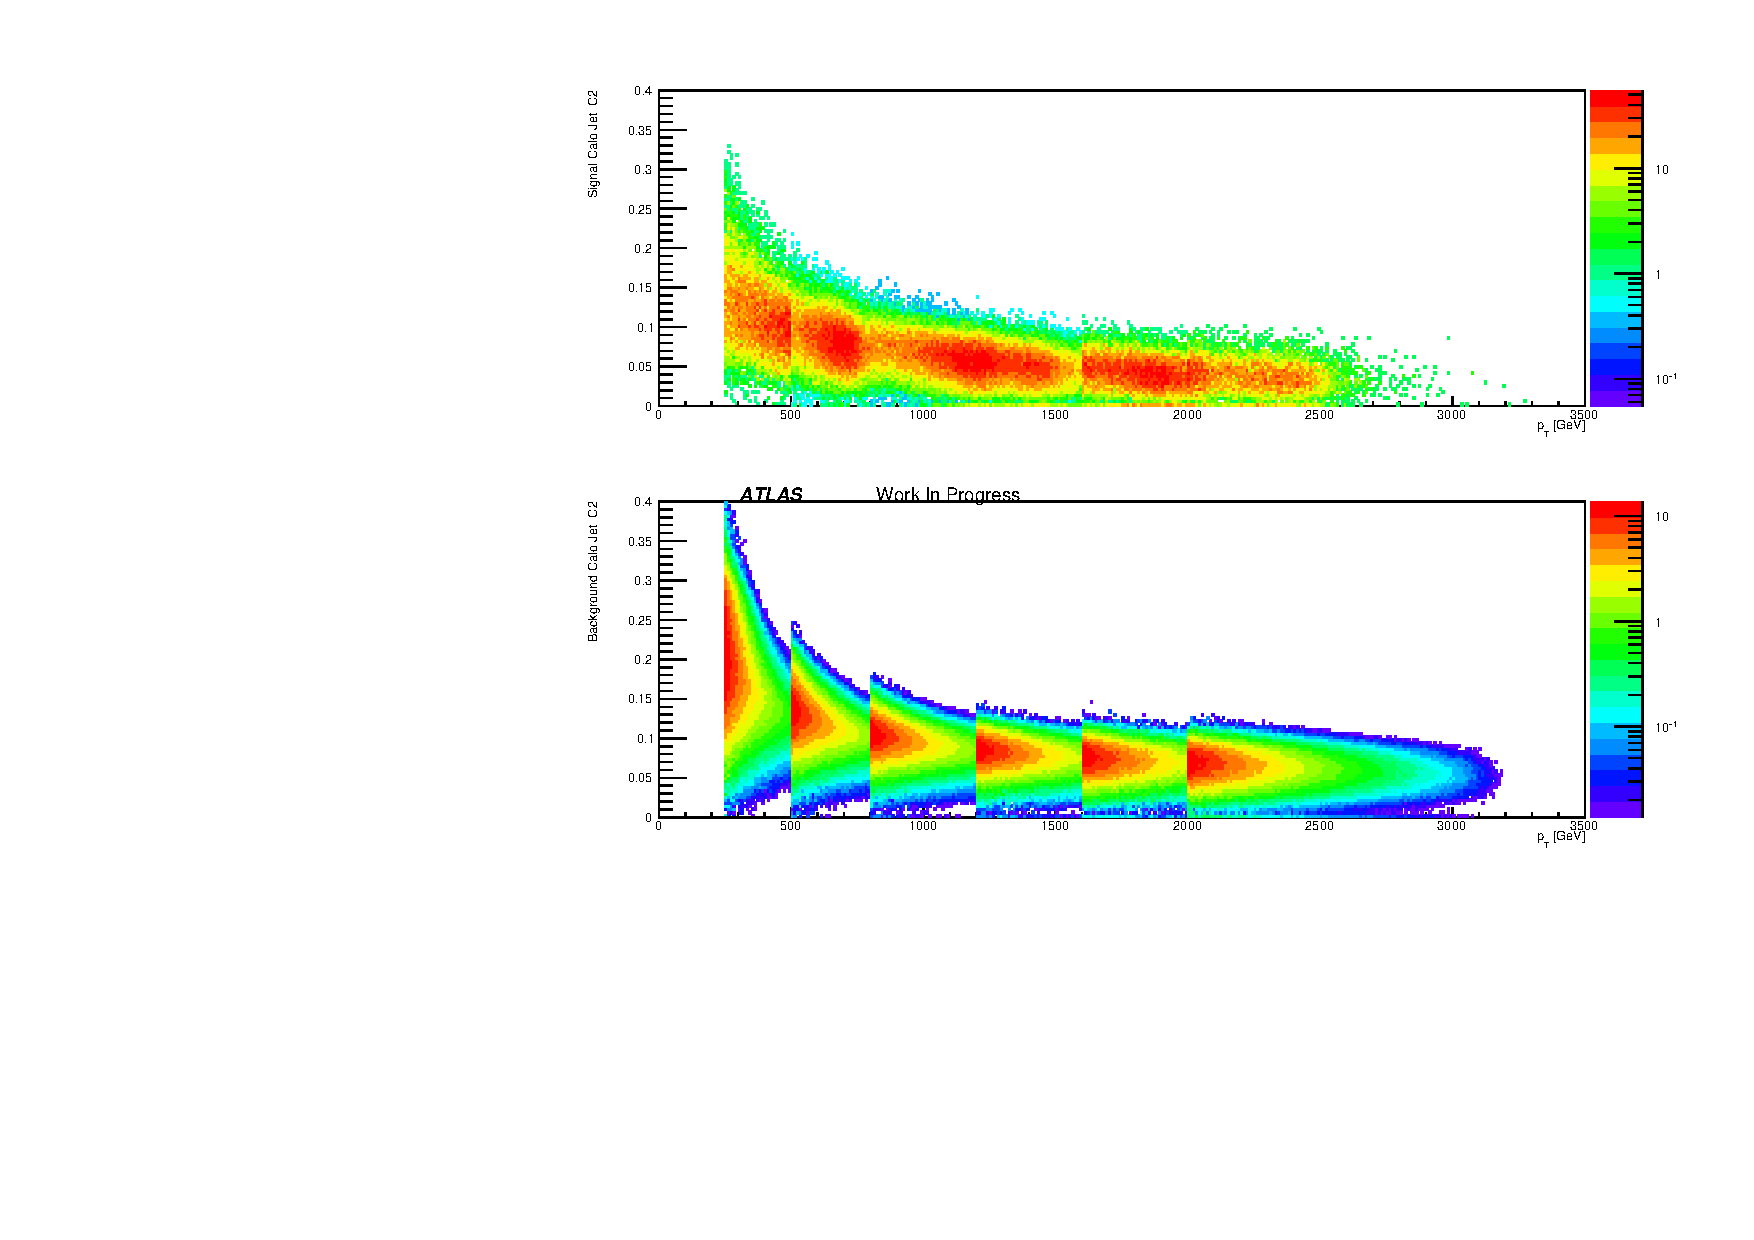
\includegraphics[width=0.5\textwidth]{sascha_input/plots/W/beta1/scatter_plots/scatter_h_scatter_reco_C2.pdf}
\bigskip
\includegraphics[width=0.5\textwidth]{sascha_input/plots/W/beta1/scatter_plots/scatter_h_scatter_assisted_tj_C2.pdf} 
\caption{\footnotesize{Correlation between C2 at $\beta=1$ and $p_{\mathrm{T}}$ applied on $W$ boson signal (above) and QCD background (below) for calorimeter (left) and TAS (right).}}\label{fig:correlation_C2}
\end{figure}

\begin{figure}[htp]
\includegraphics[width=0.5\textwidth]{sascha_input/plots/W/beta1/scatter_plots/scatter_h_scatter_reco_D2.pdf}
\bigskip
\includegraphics[width=0.5\textwidth]{sascha_input/plots/W/beta1/scatter_plots/scatter_h_scatter_assisted_tj_D2.pdf} 
\caption{\footnotesize{Correlation between D2 at $\beta=1$ and $p_{\mathrm{T}}$ applied on $W$ boson signal (above) and QCD background (below) for calorimeter (left) and TAS (right).}}\label{fig:correlation_D2}
\end{figure}

\begin{figure}[htp]
\includegraphics[width=0.5\textwidth]{sascha_input/plots/W/beta1/scatter_plots/scatter_h_scatter_reco_nSub21.pdf}
\bigskip
\includegraphics[width=0.5\textwidth]{sascha_input/plots/W/beta1/scatter_plots/scatter_h_scatter_assisted_tj_nSub21.pdf} 
\caption{\footnotesize{Correlation between $\tau_{21}$ at $\beta=1$ and $p_{\mathrm{T}}$ applied on $W$ boson signal (above) and QCD background (below) for calorimeter (left) and TAS (right).}}\label{fig:correlation_tau21}
\end{figure}

\subsubsection{Performance for Higgs boson tagging}\label{subsubsec:higgs_beta1}
The Higgs boson is heavier than the $W$ or $Z$ boson, resulting in a higher angular separation of the jet constituents considering the rule of thumb $\delta R \sim \frac{2m}{p_T}$ for decay products. As a result, angular resolution effects won't have the same impact as for the $W$ boson. This can be verified by the performance of track-based variables in the ROCs found in Figure \ref{fig:ROC_higgs_nSub21}.

For Higgs boson tagging and an angular weight of $\beta=1$, found were no distinct improvements with TAS or tracks compared to calorimeter clusters. The C2 variable performs better with calorimeter clusters, D2 yields an equal QCD discrimination with TAS and calorimeter clusters. The n-Subjettiness ratio $\tau_{21}$ benefits from TAS in some $p_{\mathrm{T}}$ regions, while the calorimeter pendant performs better in the other regions. Furthermore, tracks and TAS perform comparable over the whole studied $p_{\mathrm{T}}$ range. 
\begin{figure}[htp]
\includegraphics[width=0.3\textwidth]{sascha_input/plots/Higgs/ROC/Beta1/ROC_ALL_h_recoJet_C2_bin2.pdf} 
\includegraphics[width=0.3\textwidth]{sascha_input/plots/Higgs/ROC/Beta1/ROC_ALL_h_recoJet_D2_bin2.pdf} 
\includegraphics[width=0.3\textwidth]{sascha_input/plots/Higgs/ROC/Beta1/ROC_ALL_h_recoJet_nSub21_bin2.pdf}
\bigskip
\includegraphics[width=0.3\textwidth]{sascha_input/plots/Higgs/ROC/Beta1/ROC_ALL_h_recoJet_C2_bin5.pdf} \hspace{6mm}
\includegraphics[width=0.3\textwidth]{sascha_input/plots/Higgs/ROC/Beta1/ROC_ALL_h_recoJet_D2_bin5.pdf} \hspace{6mm}
\includegraphics[width=0.3\textwidth]{sascha_input/plots/Higgs/ROC/Beta1/ROC_ALL_h_recoJet_nSub21_bin5.pdf}
\caption{\footnotesize{ROCs showing QCD rejection against Higgs boson efficiency for tracks, TAS and colorimeter. C2 (left), D2 (middle) and $\tau_{21}$ (right) at $\beta=1$. Shown is the energy range between 500-800 GeV (top) and 1600-2000 GeV (bottom). The numbers in the legend second $p_{\mathrm{T}}$ bin (left) and highest bin (right). The numbers in the legend indicate the achieved background rejection at 50\% signal efficiency.}}\label{fig:ROC_higgs_nSub21}
\end{figure}

\subsubsection{Performance for Top quark tagging}
The top quark features a characteristic three body decay and a very high mass around $173 \, \text{GeV}$. Studied here is the n-Subjettiness ratio $\tau_{32}$ to distinguish the three prong like top quark jets and QCD background jets.

The ROCs in Figure \ref{fig:ROC_top} show the accompanying improvements in the separation power of $\tau_{32}$ possible with TAS. Tagging tops quark events with $\tau_{32}$ is found to greatly benefit from the excellent angular resolution of tracks. This is especially the case for high $p_{\mathrm{T}}$ where the limitation of the calorimeter cell size clearly diminishes the possible identification of three distinct substructures inside a large-R jet. The enhancements are not as articulated for the low $p_{\mathrm{T}}$ regions, nevertheless TAS $\tau_{32}$ performs here at least equally well as calorimeter $\tau_{32}$. Furthermore, tracks are observed to perform slightly worse in comparison with TAS for the lower $p_{\mathrm{T}}$ regions, but match the TAS performance for very large boosts as expected.
\begin{figure}[htp]
\includegraphics[width=0.5\textwidth]{sascha_input/plots/Top/beta1/ROC_ALL_h_recoJet_nSub32_bin2.pdf} \hspace{1mm}
\includegraphics[width=0.5\textwidth]{sascha_input/plots/Top/beta1/ROC_ALL_h_recoJet_nSub32_bin3.pdf}
\bigskip
\includegraphics[width=0.5\textwidth]{sascha_input/plots/Top/beta1/ROC_ALL_h_recoJet_nSub32_bin5.pdf} \hspace{1mm}
\includegraphics[width=0.5\textwidth]{sascha_input/plots/Top/beta1/ROC_ALL_h_recoJet_nSub32_bin6.pdf}
\caption{\footnotesize{ROCs showing QCD rejection against top quark efficiency for tracks, TAS and colorimeter $\tau_{32}$ at $\beta=1$, $p_{\mathrm{T}}$ ordering from upper left to lower right.}}\label{fig:ROC_top}
\end{figure}





\subsection{Optimisation of $\beta$}
The observed background rejection of variables calculated with TAS and tracks is at least as high as of calorimeter cluster based variables due to the high angular resolution of tracks. Therefore, studied are the effects of a higher weighting of the angular part of the substructure variables. For completeness, considered as well is a lower weighting. Previous studies of default calorimeter variables for $W$ boson tagging, see e.g. Reference \cite{bib:w_tagging}, found $\beta=1$ to maximize the separation power of calorimeter variables.

A scan over the values $\beta= 0.5, 1, 1.7, 2, 3$ is performed in order to identify the best variables for the specific scenarios of tagging $W$ boson, Higgs boson or top quark jets. The background rejections, achieved at the $50\,\%$ working point after mass cut and tagging are summarized in tables. The corresponding ROCs can be found in Appendix \ref{chp:best_ROC}. Pseudo-experiments were used to propagate the uncertainties on the signal and background distributions due to the finite size of the MC samples to the background rejections. 

\subsubsection{Optimisation for $W$ boson jets}
The results of the optimisation for $W$ boson jets are shown in Table \ref{table:w_scan}. As expected, tracks and TAS perform visibly worse with a low angular weighting. For higher values of $\beta$, tracks and TAS gain in separation power, verifying the significance of the angular part for track based variables. Nevertheless, the separation is observed to degrade for angular weightings too high compared to the $p_{\mathrm{T}}$ part, here $\beta=3$.

A $\beta$ of around 2 maximizes the separation power of tracks and TAS. The advantages of $\beta=2$ compared to $\beta=1$ are found at higher $p_{\mathrm{T}}$ values, minor losses are visible in the lowest energy regions. A slightly lower value of $\beta=1.7$ was able to retain the great background rejection of a large angular weighting at high $p_{\mathrm{T}}$ while still performing well at lower energies. Variables calculated with clusters are not as sensitive to a variation of the angular weighting.

C2 is found to be relatively insensitive to the track assisting, whereas separation with $\tau_{21}$ and D2 (for lower energies) is visibly poorer with tracks compared to TAS.  Starting around $1200\;$GeV, tracks perform comparably and for even higher energies equally well as TAS due to the rising amount of large-R jets with only one sub-jet. Comparing variables independently for the different inputs, $\tau_{21}$ performs worse than C2 and D2. However, e.g. $\tau_{21,\: \text{TAS}}$ can outperform $\text{C2}_{\text{calo}}$ and $\text{D2}^{\text{calo}}$.

The variables achieving the highest background rejections for $W$ boson tagging are $\text{D2}_{\text{TAS}}^{(\beta=1.7)}$ and $\text{C2}_{\text{TAS}}^{(\beta=1.7)}$, depending on the energy. D2 cut values were shown to be more $p_{\mathrm{T}}$ robust, C2 could also be used with tracks instead of TAS, which saves the assistance. For TAS variables, uncertainties on the sub-jets, whose derivation is being worked at, need to be propagated while tracks feature already well-known uncertainties.

\begin{sidewaystable}[]
\centering
\resizebox{22cm}{!}{%
\begin{tabular}{llllllllllllllll}
 \multicolumn{1}{l||}{\textbf{Calorimeter}} &  &  & C2 &  & \multicolumn{1}{l||}{} &  &  & D2 &  & \multicolumn{1}{l||}{} &  &  & $\tau_{21}$ &  & \multicolumn{1}{l|}{} \\ \hline
\multicolumn{1}{l||}{$p_{\mathrm{T}} \, \text{[GeV]}$} &  \multicolumn{1}{l|}{$\beta=0.5$} & \multicolumn{1}{l|}{1} & \multicolumn{1}{l|}{1.7} & \multicolumn{1}{l|}{2} & \multicolumn{1}{l||}{3} & \multicolumn{1}{l|}{$\beta=0.5$} & \multicolumn{1}{l|}{1} & \multicolumn{1}{l|}{1.7} & \multicolumn{1}{l|}{2} & \multicolumn{1}{l||}{3} & \multicolumn{1}{l|}{$\beta=0.5$} & \multicolumn{1}{l|}{1} & \multicolumn{1}{l|}{1.7} & \multicolumn{1}{l|}{2} & \multicolumn{1}{l|}{3} \\ \hline \hline
\multicolumn{1}{l||}{250 - 500} & 	\multicolumn{1}{l|}{29.7(1.5)} & 	 \multicolumn{1}{l|}{31.7(1.9)} & 		\multicolumn{1}{l|}{31.4(1.6)} & 	 \multicolumn{1}{l|}{30.7(1.9)} &     \multicolumn{1}{l||}{28.5(1.4)} & 	\multicolumn{1}{l|}{27.2(2.0)}& 	\multicolumn{1}{l|}{35.0(2.0)} & 		\multicolumn{1}{l|}{33.0(1.8)} & 		\multicolumn{1}{l|}{31.3(1.7)} & 	 \multicolumn{1}{l||}{25.7(1.2)} & 	   \multicolumn{1}{l|}{33.1(1.8)} & \multicolumn{1}{l|}{27.6(1.3)} & \multicolumn{1}{l|}{26.2(1.4)} & \multicolumn{1}{l|}{25.1(1.2)} & \multicolumn{1}{l|}{22.4(0.8)} \\
\multicolumn{1}{l||}{500 - 800} & 	\multicolumn{1}{l|}{44.2(1.8)} & 	 \multicolumn{1}{l|}{50.1(2.0)} & 		\multicolumn{1}{l|}{49.6(1.9)} & 	 \multicolumn{1}{l|}{48.6(1.8)} & 	  \multicolumn{1}{l||}{42.6(1.9)} &  	\multicolumn{1}{l|}{40.3(2.2)} & 	\multicolumn{1}{l|}{55.3(2.6)} & 		\multicolumn{1}{l|}{56.3(2.4)} & 		\multicolumn{1}{l|}{52.5(2.1)} & 	 \multicolumn{1}{l||}{39.3(1.3)} & 	   \multicolumn{1}{l|}{49.4(2.0)} & \multicolumn{1}{l|}{41.1(1.4)} & \multicolumn{1}{l|}{43.3(1.7)} & \multicolumn{1}{l|}{41.3(1.6)} & \multicolumn{1}{l|}{36.1(1.2)} \\
\multicolumn{1}{l||}{800 - 1200} & 	\multicolumn{1}{l|}{32.0(1.5)} & 	 \multicolumn{1}{l|}{37.5(1.7)} & 		\multicolumn{1}{l|}{35.4(1.5)} & 	 \multicolumn{1}{l|}{33.4(1.5)} & 	  \multicolumn{1}{l||}{26.8(0.9)} &  	\multicolumn{1}{l|}{34.0(2.1)} & 	\multicolumn{1}{l|}{41.1(2.0)} & 		\multicolumn{1}{l|}{38.5(1.6)} & 		\multicolumn{1}{l|}{34.9(1.3)} & 	 \multicolumn{1}{l||}{25.4(0.7)} & 	   \multicolumn{1}{l|}{30.5(1.2)} & \multicolumn{1}{l|}{30.9(1.2)} & \multicolumn{1}{l|}{33.8(1.4)} & \multicolumn{1}{l|}{32.5(1.3)} & \multicolumn{1}{l|}{28.1(0.9)} \\
\multicolumn{1}{l||}{1200 - 1600} & \multicolumn{1}{l|}{30.1(1.3)} & 	 \multicolumn{1}{l|}{34.4(1.8)} & 		\multicolumn{1}{l|}{29.4(1.3)} & 	 \multicolumn{1}{l|}{26.8(1.0)} & 	  \multicolumn{1}{l||}{20.7(0.8)} &  	\multicolumn{1}{l|}{34.1(1.8)} & 	\multicolumn{1}{l|}{38.1(1.9)} & 		\multicolumn{1}{l|}{31.4(1.4)} & 		\multicolumn{1}{l|}{27.6(1.2)} & 	 \multicolumn{1}{l||}{19.3(0.5)} & 	   \multicolumn{1}{l|}{23.1(0.9)} & \multicolumn{1}{l|}{27.3(1.)} & \multicolumn{1}{l|}{31.1(1.2)} & \multicolumn{1}{l|}{29.9(1.3)} & \multicolumn{1}{l|}{24.8(0.9)} \\
\multicolumn{1}{l||}{1600 - 2000} & \multicolumn{1}{l|}{20.9(1.3)} & 	 \multicolumn{1}{l|}{22.4(1.5)} & 		\multicolumn{1}{l|}{18.2(1.2)} & 	 \multicolumn{1}{l|}{16.5(0.9)} & 	  \multicolumn{1}{l||}{12.9(0.6)} &  	\multicolumn{1}{l|}{26.4(1.7)} & 	\multicolumn{1}{l|}{25.4(1.3)} & 		\multicolumn{1}{l|}{19.3(1.1)} & 		\multicolumn{1}{l|}{16.9(0.9)} & 	 \multicolumn{1}{l||}{11.9(0.5)} & 	   \multicolumn{1}{l|}{16.4(1.0)} & \multicolumn{1}{l|}{19.1(1.1)} & \multicolumn{1}{l|}{21.1(1.1)} & \multicolumn{1}{l|}{19.9(1.0)} & \multicolumn{1}{l|}{16.0(0.9)} \\
\multicolumn{1}{l||}{$>2000$} & 	\multicolumn{1}{l|}{16.9(1.4)} & 	 \multicolumn{1}{l|}{18.7(1.4)} & 		\multicolumn{1}{l|}{14.1(0.9)} & 	 \multicolumn{1}{l|}{12.6(0.8)} & 	  \multicolumn{1}{l||}{9.9(0.7)} & 		\multicolumn{1}{l|}{23.3(1.9)} & 	\multicolumn{1}{l|}{21.9(1.7)} & 		\multicolumn{1}{l|}{15.7(1.1)} & 		\multicolumn{1}{l|}{13.5(0.9)} & 	 \multicolumn{1}{l||}{9.2(0.4)} & 	   \multicolumn{1}{l|}{12.3(1.1)} & \multicolumn{1}{l|}{15.5(1.1)} & \multicolumn{1}{l|}{17.2(1.2)} & \multicolumn{1}{l|}{15.7(1.1)} & \multicolumn{1}{l|}{11.9(0.8)} \\ \hline
 &  &  &  &  &  &  &  &  &  &  &  &  &  &  &  \\
 \multicolumn{1}{l||}{\textbf{TAS}} &  &  & C2 &  & \multicolumn{1}{l||}{} &  &  & D2 &  & \multicolumn{1}{l||}{} &  &  & $\tau_{21}$ &  & \multicolumn{1}{l|}{} \\ \hline
\multicolumn{1}{l||}{$p_{\mathrm{T}} \, \text{[GeV]}$}   &  \multicolumn{1}{l|}{  $\beta=0.5$} & \multicolumn{1}{l|}{ 1} & \multicolumn{1}{l|}{1.7} &   \multicolumn{1}{l|}{ 2} &  \multicolumn{1}{l||}{ 3} & \multicolumn{1}{l|}{ $\beta=0.5$} &  \multicolumn{1}{l|}{ 1} & 	\multicolumn{1}{l|}{ 1.7} & 	\multicolumn{1}{l|}{ 2} & \multicolumn{1}{l||}{ 3} & \multicolumn{1}{l|}{  $\beta=0.5$} & \multicolumn{1}{l|}{ 1} & \multicolumn{1}{l|}{ 1.7} &  \multicolumn{1}{l|}{ 2} & \multicolumn{1}{l|}{ 3} \\ \hline \hline
\multicolumn{1}{l||}{250 - 500} & 	\multicolumn{1}{l|}{29.4(1.9)} & \multicolumn{1}{l|}{30.1(1.9)} & \multicolumn{1}{l|}{28.9(1.5)} & 				     	\multicolumn{1}{l|}{28.5(1.3)} & 						\multicolumn{1}{l||}{27.7(1.3)} & \multicolumn{1}{l|}{28.6(2.0)} & \multicolumn{1}{l|}{37.7(2.1)} & 		\multicolumn{1}{l|}{35.4(2.3)} & 					\multicolumn{1}{l|}{33.4(2.0)} & 	\multicolumn{1}{l||}{29.4(1.2)} & 					\multicolumn{1}{l|}{36.2(2.2)} & 	\multicolumn{1}{l|}{31.5(1.6)} & \multicolumn{1}{l|}{26.8(1.3)} & \multicolumn{1}{l|}{25.4(1.4)} & \multicolumn{1}{l|}{24.0(1.0)} \\
\multicolumn{1}{l||}{500 - 800} & 	\multicolumn{1}{l|}{48.2(2.0)} & \multicolumn{1}{l|}{55.5(2.7)} & \multicolumn{1}{l|}{58.6(2.6)} & 				     	\multicolumn{1}{l|}{59.1(2.7)} & 						\multicolumn{1}{l||}{56.8(2.0)} & \multicolumn{1}{l|}{42.8(2.3)} & \multicolumn{1}{l|}{67.2(3.1)} & 						\multicolumn{1}{l|}{67.6(3.2)} & 	\multicolumn{1}{l|}{63.7(3.0)} & 	\multicolumn{1}{l||}{52.6(2.3)} & 					\multicolumn{1}{l|}{55.7(2.6)} & 	\multicolumn{1}{l|}{51.9(2.1)} & \multicolumn{1}{l|}{45.5(2.0)} & \multicolumn{1}{l|}{44.0(1.9)} & \multicolumn{1}{l|}{41.3(1.5)} \\
\multicolumn{1}{l||}{800 - 1200} & 	\multicolumn{1}{l|}{31.0(1.2)} & \multicolumn{1}{l|}{44.6(1.9)} & \multicolumn{1}{l|}{54.6(2.8)} & 				     	\multicolumn{1}{l|}{55.2(2.8)} & 		\multicolumn{1}{l||}{53.0(3.2)} & \multicolumn{1}{l|}{26.1(1.3)} & \multicolumn{1}{l|}{47.6(2.3)} & 						\multicolumn{1}{l|}{54.9(2.4)} & 					\multicolumn{1}{l|}{52.6(2.8)} & 	\multicolumn{1}{l||}{43.1(1.5)} & 					\multicolumn{1}{l|}{36.4(1.8)} & 	\multicolumn{1}{l|}{37.3(1.7)} & \multicolumn{1}{l|}{36.2(1.8)} & \multicolumn{1}{l|}{36.2(1.6)} & \multicolumn{1}{l|}{35.5(1.6)} \\
\multicolumn{1}{l||}{1200 - 1600} & \multicolumn{1}{l|}{20.9(0.7)} & \multicolumn{1}{l|}{39.1(1.9)} & \multicolumn{1}{l|}{53.8(2.6)} & 				     	\multicolumn{1}{l|}{55.1(3.0)} & 		\multicolumn{1}{l||}{50.1(1.6)} & \multicolumn{1}{l|}{22.7(1.4)} & \multicolumn{1}{l|}{42.1(2.4)} & 						\multicolumn{1}{l|}{50.8(1.8)} & 					\multicolumn{1}{l|}{49.6(2.3)} & 	\multicolumn{1}{l||}{41.1(1.2)} & 					\multicolumn{1}{l|}{27.9(1.3)} & 	\multicolumn{1}{l|}{31.4(1.5)} & \multicolumn{1}{l|}{33.4(1.6)} & \multicolumn{1}{l|}{34.0(2.0)} & \multicolumn{1}{l|}{33.0(1.8)} \\
\multicolumn{1}{l||}{1600 - 2000} & \multicolumn{1}{l|}{16.7(0.7)} & \multicolumn{1}{l|}{36.9(2.9)} & \multicolumn{1}{l|}{50.9(4.3)} &    \multicolumn{1}{l|}{50.3(4.4)} & 						\multicolumn{1}{l||}{42.2(2.4)} & \multicolumn{1}{l|}{18.7(1.7)} & \multicolumn{1}{l|}{32.7(3.3)} & 						\multicolumn{1}{l|}{37.8(2.0)} & 					\multicolumn{1}{l|}{36.1(2.4)} & 	\multicolumn{1}{l||}{28.7(1.2)} & 					\multicolumn{1}{l|}{20.5(1.2)} & 	\multicolumn{1}{l|}{24.8(1.6)} & \multicolumn{1}{l|}{26.1(2.0)} & \multicolumn{1}{l|}{26.5(2.0)} & \multicolumn{1}{l|}{25.4(2.0)} \\
\multicolumn{1}{l||}{$>2000$} & 	\multicolumn{1}{l|}{11.6(0.6)} & \multicolumn{1}{l|}{31.2(3.2)} & \multicolumn{1}{l|}{46.1(4.7)} &    \multicolumn{1}{l|}{45.5(5.2)} & 						\multicolumn{1}{l||}{35.5(3.8)} & \multicolumn{1}{l|}{17.8(2.0)} & \multicolumn{1}{l|}{33.0(4.0)} & 						\multicolumn{1}{l|}{36.3(2.0)} & 					\multicolumn{1}{l|}{34.0(2.5)} & 	\multicolumn{1}{l||}{27.4(1.3)} & 					\multicolumn{1}{l|}{16.4(1.3)} & 	\multicolumn{1}{l|}{22.3(2.0)} & \multicolumn{1}{l|}{24.2(2.2)} & \multicolumn{1}{l|}{24.4(2.5)} & \multicolumn{1}{l|}{21.8(2.4)} \\ \hline
 &  &  &  &  &  &  &  &  &  &  &  &  &  &  &  \\
 \multicolumn{1}{l||}{\textbf{Tracks}} &  &  & C2 &  & \multicolumn{1}{l||}{} &  &  & D2 &  & \multicolumn{1}{l||}{} &  &  & $\tau_{21}$ &  & \multicolumn{1}{l|}{} \\ \hline
\multicolumn{1}{l||}{$p_{\mathrm{T}} \, \text{[GeV]}$}  & \multicolumn{1}{l|}{$\beta=0.5$} & \multicolumn{1}{l|}{1} & \multicolumn{1}{l|}{1.7} & \multicolumn{1}{l|}{2} & \multicolumn{1}{l||}{3} & \multicolumn{1}{l|}{$\beta=0.5$} & \multicolumn{1}{l|}{1} & \multicolumn{1}{l|}{1.7} & \multicolumn{1}{l|}{2} & \multicolumn{1}{l||}{3} & \multicolumn{1}{l|}{$\beta=0.5$} & \multicolumn{1}{l|}{1} & \multicolumn{1}{l|}{1.7} & \multicolumn{1}{l|}{2} & \multicolumn{1}{l|}{3} \\ \hline \hline
\multicolumn{1}{l||}{250 - 500} & 	\multicolumn{1}{l|}{27.1(1.2)} & \multicolumn{1}{l|}{28.1(1.5)} & \multicolumn{1}{l|}{28.7(1.9)} 						& \multicolumn{1}{l|}{28.7(1.9)} 					& \multicolumn{1}{l||}{28.2(1.7)} & \multicolumn{1}{l|}{21.6(1.2)} & \multicolumn{1}{l|}{28.9(2.0)} & \multicolumn{1}{l|}{29.5(1.8)} 		& \multicolumn{1}{l|}{29.1(1.6)} & \multicolumn{1}{l||}{28.1(1.3)} & \multicolumn{1}{l|}{28.7(1.8)} & \multicolumn{1}{l|}{28.0(1.7)} & \multicolumn{1}{l|}{25.6(1.3)} & \multicolumn{1}{l|}{25.1(1.3)} & \multicolumn{1}{l|}{24.2(0.9)} \\
\multicolumn{1}{l||}{500 - 800} & 	\multicolumn{1}{l|}{46.5(1.9)} & \multicolumn{1}{l|}{52.9(2.4)} & \multicolumn{1}{l|}{57.7(2.6)} 						& \multicolumn{1}{l|}{58.1(2.7)} 	& \multicolumn{1}{l||}{55.8(2.5)} & \multicolumn{1}{l|}{30.1(1.8)} & \multicolumn{1}{l|}{46.8(2.4)} & \multicolumn{1}{l|}{53.4(2.2)} 						& \multicolumn{1}{l|}{52.1(2.3)} & \multicolumn{1}{l||}{46.6(1.7)} & \multicolumn{1}{l|}{46.1(2.3)} & \multicolumn{1}{l|}{44.9(1.8)} & \multicolumn{1}{l|}{41.7(2.1)} & \multicolumn{1}{l|}{40.6(1.8)} & \multicolumn{1}{l|}{39.2(1.5)} \\
\multicolumn{1}{l||}{800 - 1200} & 	\multicolumn{1}{l|}{30.3(1.1)} & \multicolumn{1}{l|}{44.5(2.2)} & \multicolumn{1}{l|}{54.8(2.8)} 						& \multicolumn{1}{l|}{56.4(3.0)} 	& \multicolumn{1}{l||}{53.7(3.6)} & \multicolumn{1}{l|}{24.5(1.5)} & \multicolumn{1}{l|}{42.3(2.3)} & \multicolumn{1}{l|}{48.6(2.5)} 						& \multicolumn{1}{l|}{47.5(1.2)} & \multicolumn{1}{l||}{42.4(1.2)} & \multicolumn{1}{l|}{34.5(1.6)} & \multicolumn{1}{l|}{36.2(1.8)} & \multicolumn{1}{l|}{36.0(1.8)} & \multicolumn{1}{l|}{36.2(1.8)} & \multicolumn{1}{l|}{35.7(1.5)} \\
\multicolumn{1}{l||}{1200 - 1600} & \multicolumn{1}{l|}{20.7(0.6)} & \multicolumn{1}{l|}{39.0(1.9)} & \multicolumn{1}{l|}{54.2(2.7)} 						& \multicolumn{1}{l|}{55.5(3.3)} 	& \multicolumn{1}{l||}{50.9(1.7)} & \multicolumn{1}{l|}{22.7(1.3)} & \multicolumn{1}{l|}{41.0(2.2)} & \multicolumn{1}{l|}{50.0(1.6)} 						& \multicolumn{1}{l|}{47.6(2.2)} & \multicolumn{1}{l||}{41.4(1.2)} & \multicolumn{1}{l|}{27.7(1.2)} & \multicolumn{1}{l|}{31.3(1.4)} & \multicolumn{1}{l|}{33.3(1.6)} & \multicolumn{1}{l|}{33.9(1.7)} & \multicolumn{1}{l|}{33.2(1.8)} \\
\multicolumn{1}{l||}{1600 - 2000} & \multicolumn{1}{l|}{16.6(0.7)} & \multicolumn{1}{l|}{36.7(2.3)} & \multicolumn{1}{l|}{51.7(5.2)} 		& \multicolumn{1}{l|}{51.6(4.0)} 					& \multicolumn{1}{l||}{43.1(2.3)} & \multicolumn{1}{l|}{18.5(1.7)} & \multicolumn{1}{l|}{32.1(3.0)} & \multicolumn{1}{l|}{37.0(1.9)} 						& \multicolumn{1}{l|}{35.9(2.3)} & \multicolumn{1}{l||}{29.3(1.2)} & \multicolumn{1}{l|}{20.5(1.3)} & \multicolumn{1}{l|}{24.6(1.7)} & \multicolumn{1}{l|}{26.2(1.8)} & \multicolumn{1}{l|}{26.7(2.0)} & \multicolumn{1}{l|}{25.9(2.2)} \\
\multicolumn{1}{l||}{$>2000$} & 	\multicolumn{1}{l|}{11.6(0.5)} & \multicolumn{1}{l|}{31.5(3.0)} & \multicolumn{1}{l|}{46.8(5.7)} 		& \multicolumn{1}{l|}{46.0(4.2)} 					& \multicolumn{1}{l||}{36.1(4.3)} & \multicolumn{1}{l|}{17.8(2.2)} & \multicolumn{1}{l|}{33.0(3.3)} & \multicolumn{1}{l|}{35.9(2.1)} 						& \multicolumn{1}{l|}{34.2(2.6)} & \multicolumn{1}{l||}{28.1(1.0)} & \multicolumn{1}{l|}{16.4(1.4)} & \multicolumn{1}{l|}{22.5(1.8)} & \multicolumn{1}{l|}{24.5(2.4)} & \multicolumn{1}{l|}{24.7(2.6)} & \multicolumn{1}{l|}{22.2(2.6)} \\ \hline
\end{tabular}}
\caption{Listing of the QCD background rejection for $W$ boson signal achieved with C2, D2 and $\tau_{21}$ together with different angular weightings $\beta$ and for calorimeter cluster, tracks and TAS.}\label{table:w_scan}
\end{sidewaystable}

Shown in Figure \ref{fig:w_cut} are the cut values for $50\,\%$ and $25\,\%$ signal efficiency for $\text{D2}_{\text{TAS}}^{(\beta=1.7)}$ and $\text{C2}_{\text{TAS}}^{(\beta=1.7)}$. $\text{D2}_{\text{TAS}}^{(\beta=1.7)}$. As for the default cluster variables, the $\text{D2}_{\text{TAS}}^{(\beta=1.7)}$ cut is more $p_{\mathrm{T}}$ robust than the cut on $\text{C2}_{\text{TAS}}^{(\beta=1.7)}$. 
\begin{figure}
\includegraphics[width=0.5\textwidth]{sascha_input/plots/W/cut_value/c2_tas17.pdf} \hspace{1mm}
\includegraphics[width=0.5\textwidth]{sascha_input/plots/W/cut_value/d2_tas17.pdf}	
\caption{\footnotesize{Cut values for $\text{C2}_{\text{TAS}}^{(\beta=1.7)}$ (left) and $\text{D2}_{\text{TAS}}^{(\beta=1.7)}$ (right) to achieve $50\,\%$ and $25\,\%$ $W$ boson efficiency.}}\label{fig:w_cut}
\end{figure}
%The steeper $50\,\%$ working point curves can be explained with the signal distributions, see Figure \ref{fig:w_distris}. The signal distributions rise steeply for low values, which doesn't chance considerably with rising $p_{\mathrm{T}}$. The right-handed tail of the distributions in contrast becomes increasingly narrow for $\text{C2}_{\text{TAS}}^{(\beta=1.7)}$ and broader for $\text{D2}_{\text{TAS}}^{(\beta=1.7)}$. Therefore, the curves for the $50\,\%$ cut feature a larger slope as the $25\,\%$ cut, which already given by the sharp rise. 

Table \ref{table:w_improvement} lists the background rejections for $\text{D2}_{\text{TAS}}^{(\beta=1.7)}$, $\text{C2}_{\text{TAS}}^{(\beta=1.7)}$ and the currently used $\text{D2}^{\beta=1}_{calo}$ along with the corresponding improvements. For lower energies, $\text{D2}_{\text{TAS}}^{(\beta=1.7)}$ is the best choice. For very high boosts of the $W$ boson, $\text{C2}_{\text{TAS}}^{(\beta=1.7)}$ performs superior, especially for $25\,\%$ $\epsilon_{signal}$, where the background rejection with $\text{C2}_{\text{TAS}}^{(\beta=1.7)}$ is around 3.5 times as large as the QCD rejection with $\text{D2}^{(\beta=1)}_{\text{calo}}$.
%\begin{figure}[]
%\includegraphics[width=0.25\textwidth]{sascha_input/plots/W/cut_value/h_assisted_tj_C2_17_bin1.pdf} 
%\includegraphics[width=0.25\textwidth]{sascha_input/plots/W/cut_value/h_assisted_tj_C2_17_bin4.pdf} 
%\includegraphics[width=0.25\textwidth]{sascha_input/plots/W/cut_value/h_assisted_tj_D2_17_bin1.pdf} 
%\includegraphics[width=0.25\textwidth]{sascha_input/plots/W/cut_value/h_assisted_tj_D2_17_bin4.pdf} 
%\caption{\footnotesize{$W$ boson signal and QCD background distributions for C2 TAS at $\beta=1.7$ (above) and D2 TAS at $\beta=1.7$ (below) for the %first (left) and fourth (right) $p_{\mathrm{T}}$ bin.}}\label{fig:w_distris}
%\end{figure}
These enormous improvements at lower $\epsilon_{signal}$ are due to the signal distributions for TAS and tracks rising much steeper than for clusters. The tail to higher, background like values in contrast, is more comparable, leading to an alignment of the background rejection for very large $\epsilon_{signal}$. The improvements due to TAS lie around $50\,\%$ for D2 and up to a $100\,\%$ for C2 in the upper $p_{\mathrm{T}}$ regions and $50\,\%$ $W$ boson efficiency. For the lower working point, they can reach $200\,\%$ for D2 and around $250\,\%$ for C2, again for very large boosts of the $W$ boson.
\begin{table}[]
\centering
\begin{tabular}{llll}
 \multicolumn{1}{l||}{\textbf{50\% $\epsilon_{signal}$}} &                                                & \textbf{W tagging}                                         &                                          \\ \hline
\multicolumn{1}{l||}{$p_{\mathrm{T}} \, \text{[GeV]}$}           & \multicolumn{1}{l|}{$\text{D2}_{\text{calo}}^{(\beta=1)}$} & \multicolumn{1}{l|}{$\text{D2}_{\text{TAS}}^{(\beta=1.7)}$} & \multicolumn{1}{l|}{$\text{C2}_{\text{TAS}}^{(\beta=1.7)}$} \\ \hline \hline
\multicolumn{1}{l||}{250 - 500}                       & \multicolumn{1}{l|}{35.0 $\pm$ 2.0}                      & \multicolumn{1}{l|}{35.4 $\pm$ 2.3 (+1 $\pm$ 9\%)}         & \multicolumn{1}{l|}{28.9 $\pm$ 1.5 (-17 $\pm$ 6\%)}        \\
\multicolumn{1}{l||}{500 - 800}                       & \multicolumn{1}{l|}{55.3 $\pm$ 2.6}                      & \multicolumn{1}{l|}{67.6 $\pm$ 3.2 (+22 $\pm$ 8\%)}        & \multicolumn{1}{l|}{58.6 $\pm$ 2.6 (+6 $\pm$ 7\%)}         \\
\multicolumn{1}{l||}{800 - 1200}                      & \multicolumn{1}{l|}{41.1 $\pm$ 2.0}                      & \multicolumn{1}{l|}{54.9 $\pm$ 2.4 (+34 $\pm$ 9\%)}        & \multicolumn{1}{l|}{54.6 $\pm$ 2.8 (+33 $\pm$ 9\%)}        \\
\multicolumn{1}{l||}{1200 - 1600}                     & \multicolumn{1}{l|}{38.1 $\pm$ 1.9}                      & \multicolumn{1}{l|}{50.8 $\pm$ 1.8 (+33 $\pm$ 8\%)}        & \multicolumn{1}{l|}{53.8 $\pm$ 2.7 (+41 $\pm$ 10\%)}        \\
\multicolumn{1}{l||}{1600 - 2000}                     & \multicolumn{1}{l|}{25.4 $\pm$ 1.3}                      & \multicolumn{1}{l|}{37.8 $\pm$ 2.0 (+49 $\pm$ 11\%)}       & \multicolumn{1}{l|}{50.9 $\pm$ 4.3 (+100 $\pm$ 20\%)}       \\
\multicolumn{1}{l||}{$>2000$}                         & \multicolumn{1}{l|}{21.9 $\pm$ 1.7}                      & \multicolumn{1}{l|}{36.3 $\pm$ 2.0 (+66 $\pm$ 16\%)}       & \multicolumn{1}{l|}{46.1 $\pm$ 4.7 (+111 $\pm$ 27\%)}       \\ \hline
                                                     &                                                &                                          &                                          \\
 \multicolumn{1}{l||}{  \textbf{25\% $\epsilon_{signal}$}} &                                                &  \textbf{W tagging}                                         &                                          \\ \hline
\multicolumn{1}{l||}{$p_{\mathrm{T}} \, \text{[GeV]}$}           & \multicolumn{1}{l|}{$\text{D2}_{\text{calo}}^{(\beta=1)}$} & \multicolumn{1}{l|}{$\text{D2}_{\text{TAS}}^{(\beta=1.7)}$} & \multicolumn{1}{l|}{$\text{C2}_{\text{TAS}}^{(\beta=1.7)}$} \\ \hline \hline
\multicolumn{1}{l||}{250 - 500}                       & \multicolumn{1}{l|}{139.6 $\pm$ 9.8}                     	& \multicolumn{1}{l|}{146.0 $\pm$ 12.4 (+5 $\pm$ 12\%)}         & \multicolumn{1}{l|}{108.2 $\pm$ 7.5 (-22 $\pm$ 8\%)}       \\
\multicolumn{1}{l||}{500 - 800}                       & \multicolumn{1}{l|}{243.7 $\pm$ 13.2}                     	& \multicolumn{1}{l|}{360.1 $\pm$ 21.1 (+48 $\pm$ 12\%)}        & \multicolumn{1}{l|}{298.4 $\pm$ 15.9 (+22 $\pm$ 9\%)}        \\
\multicolumn{1}{l||}{800 -1200}                       & \multicolumn{1}{l|}{181.0 $\pm$ 8.8}                     	& \multicolumn{1}{l|}{308.5 $\pm$ 19.3 (+70 $\pm$ 14\%)}        & \multicolumn{1}{l|}{313.2 $\pm$ 24.4 (+78 $\pm$ 16\%)}       \\
\multicolumn{1}{l||}{1200 - 1600}                     & \multicolumn{1}{l|}{156.9 $\pm$ 8.3}                     	& \multicolumn{1}{l|}{295.4 $\pm$ 17.8 (+88 $\pm$ 15\%)}        & \multicolumn{1}{l|}{354.6 $\pm$ 25.6 (+126 $\pm$ 20\%)}      \\
\multicolumn{1}{l||}{1600 - 2000}                     & \multicolumn{1}{l|}{84.6 $\pm$ 5.7}                      	& \multicolumn{1}{l|}{219.6 $\pm$ 10.9 (+160 $\pm$ 22\%)}       & \multicolumn{1}{l|}{320.5 $\pm$ 31.4 (+279 $\pm$ 45\%)}       \\
\multicolumn{1}{l||}{$>2000$}                         & \multicolumn{1}{l|}{78.9 $\pm$ 7.6}                      	& \multicolumn{1}{l|}{233.5 $\pm$ 14.7 (+196 $\pm$ 34\%)}       & \multicolumn{1}{l|}{288.4 $\pm$ 33.3 (+266 $\pm$ 55\%)}      \\ \hline
\end{tabular}

\caption{Listing of the background rejections after the jet mass cut and tagging at 50\% and 25\% $W$ boson efficiency for the identified best variables $\text{D2}_{\text{TAS}}^{(\beta=1.7)}$ \& $\text{C2}_{\text{TAS}}^{(\beta=1.7)}$ together with the improvements over the standard choice $\text{D2}_{\text{calo}}^{(\beta=1)}$}\label{table:w_improvement}
\end{table}



\subsubsection{Optimisation for Higgs boson jets}
The results of the optimisation for Higgs boson jets are shown in Table \ref{table:higgs_scan}. The study of $\beta=1$ in the Higgs boson case, see section \ref{subsubsec:higgs_beta1}, showed no improvements in the rejection of QCD events due to tracks and TAS as input. As for the $W$ boson, the performance of tracks and TAS diminishes considerably with an angular weighting of $\beta=0.5$.

No improvement of $\tau_{21}$ is observed with tracks or TAS, clusters perform equally well for lower $p_{\mathrm{T}}$ and slightly better at high energies. Again, the QCD rejection achieved with $\tau_{21}$ is exceeded by C2 and D2. The discrimination with clusters profits from a slightly higher angular weighting, although the gain is not as significant as for tracks and TAS. This consistently shows the lower sensitivity to a variation of the angular weight. The small gain is connected to the higher separation of the Higgs decay products compared to the $W$ boson case.

For boosted Higgs tagging, D2 outperforms C2 over the whole studied energy range. Values of $\beta=1.7 \& 2$ yield the highest background rejection for track and TAS based D2. $\text{D2}_{\text{TAS}}^{(\beta=1.7,2}$ and $\text{D2}_{\text{track}}^{(\beta=1.7,2}$ perform superior to $\text{D2}_{\text{calo}}$ at high boosts, due to the low angular separation of constituents, and equally well at lower enegies.

The differences between $\beta=1.7$ and $\beta=2$ are inconclusive with minor advantages at high and slight inferiorities at low $p_{\mathrm{T}}$ for $\beta=2$. Tracks perform slightly worse than TAS for lower energies but similarly better in the two highest studied $p_{\mathrm{T}}$ regions. Chosen for further examination are $\text{D2}_{\text{TAS}^{(\beta=1.7)}}$ and $\text{D2}_{\text{track}^{(\beta=1.7)}}$.

\begin{sidewaystable}[]
\centering
\hspace{-1cm}
\resizebox{22cm}{!}{%
\begin{tabular}{llllllllllllllll}
 \multicolumn{1}{l||}{\textbf{Calorimeter}}    &                                  &                           & C2                        &                           & \multicolumn{1}{l|}{}     &                                  &                           & D2                        &                           & \multicolumn{1}{l|}{}     &                                  &                           & $\tau_{21}$               &                           & \multicolumn{1}{l|}{}     \\ \hline
\multicolumn{1}{l||}{$p_{\mathrm{T}} \, [GeV]$} & \multicolumn{1}{l|}{$\beta=0.5$} & \multicolumn{1}{l|}{1}    & \multicolumn{1}{l|}{1.7}  & \multicolumn{1}{l|}{2}    & \multicolumn{1}{l||}{3}    & \multicolumn{1}{l|}{$\beta=0.5$} & \multicolumn{1}{l|}{1}    & \multicolumn{1}{l|}{1.7}  & \multicolumn{1}{l|}{2}    & \multicolumn{1}{l||}{3}    & \multicolumn{1}{l|}{$\beta=0.5$} & \multicolumn{1}{l|}{1}    & \multicolumn{1}{l|}{1.7}  & \multicolumn{1}{l|}{2}    & \multicolumn{1}{l|}{3}    \\ \hline \hline
\multicolumn{1}{l||}{250 - 500}      & \multicolumn{1}{l|}{4.6(0.1)}         & \multicolumn{1}{l|}{5.0(0.1)} & \multicolumn{1}{l|}{5.2(0.1)}  	    & \multicolumn{1}{l|}{5.3(0.1)}  & \multicolumn{1}{l||}{5.5(0.1)}  		& \multicolumn{1}{l|}{5.7(0.1)}         & \multicolumn{1}{l|}{7.3(0.2)}  & \multicolumn{1}{l|}{8.4(0.2)}  							& \multicolumn{1}{l|}{8.4(0.2)}  	    & \multicolumn{1}{l||}{8.4(0.2)}  & \multicolumn{1}{l|}{7.6(0.2)}         & \multicolumn{1}{l|}{8.0(0.2)}  & \multicolumn{1}{l|}{7.9(0.2)}  & \multicolumn{1}{l|}{7.8(0.2)}  & \multicolumn{1}{l|}{7.5(0.2)}  \\
\multicolumn{1}{l||}{500 - 800}      & \multicolumn{1}{l|}{15.7(0.3)}        & \multicolumn{1}{l|}{16.7(0.4)} & \multicolumn{1}{l|}{17.0(0.4)} 		& \multicolumn{1}{l|}{16.9(0.4)} & \multicolumn{1}{l||}{16.2(0.4)} 		& \multicolumn{1}{l|}{13.6(0.3)}        & \multicolumn{1}{l|}{16.9(0.4)} & \multicolumn{1}{l|}{17.7(0.4)} 		& \multicolumn{1}{l|}{17.2(0.4)} 						& \multicolumn{1}{l||}{15.2(0.3)} & \multicolumn{1}{l|}{16.7(0.4)}        & \multicolumn{1}{l|}{15.4(0.3)} & \multicolumn{1}{l|}{15.2(0.3)} & \multicolumn{1}{l|}{14.8(0.3)} & \multicolumn{1}{l|}{14.0(0.3)} \\
\multicolumn{1}{l||}{800 - 1200}     & \multicolumn{1}{l|}{22.1(0.5)}        & \multicolumn{1}{l|}{23.8(0.5)} & \multicolumn{1}{l|}{25.0(0.6)} 		& \multicolumn{1}{l|}{25.0(0.6)} & \multicolumn{1}{l||}{23.4(0.5)} 		& \multicolumn{1}{l|}{18.4(0.4)}        & \multicolumn{1}{l|}{23.7(0.6)} & \multicolumn{1}{l|}{26.3(0.6)} 							& \multicolumn{1}{l|}{25.6(0.6)} 		& \multicolumn{1}{l||}{22.3(0.5)} & \multicolumn{1}{l|}{22.8(0.5)}        & \multicolumn{1}{l|}{21.9(0.5)} & \multicolumn{1}{l|}{22.6(0.5)} & \multicolumn{1}{l|}{22.1(0.5)} & \multicolumn{1}{l|}{20.9(0.5)} \\
\multicolumn{1}{l||}{1200 - 1600}    & \multicolumn{1}{l|}{24.0(0.6)}        & \multicolumn{1}{l|}{26.0(0.8)} & \multicolumn{1}{l|}{26.4(0.8)} 		& \multicolumn{1}{l|}{25.9(0.7)} & \multicolumn{1}{l||}{23.0(0.6)} 		& \multicolumn{1}{l|}{19.3(0.6)}        & \multicolumn{1}{l|}{24.9(0.7)} & \multicolumn{1}{l|}{27.0(0.8)} 		& \multicolumn{1}{l|}{26.1(0.7)} 						& \multicolumn{1}{l||}{21.9(0.5)} & \multicolumn{1}{l|}{21.3(0.5)}        & \multicolumn{1}{l|}{22.6(0.6)} & \multicolumn{1}{l|}{24.0(0.6)} & \multicolumn{1}{l|}{23.7(0.6)} & \multicolumn{1}{l|}{22.2(0.5)} \\
\multicolumn{1}{l||}{1600 - 2000}    & \multicolumn{1}{l|}{12.1(0.7)}        & \multicolumn{1}{l|}{13.9(0.8)} & \multicolumn{1}{l|}{14.3(0.7)}  	& \multicolumn{1}{l|}{14.0(0.7)} & \multicolumn{1}{l||}{12.3(0.6)} 		& \multicolumn{1}{l|}{11.1(0.7)}        & \multicolumn{1}{l|}{14.1(0.9)} & \multicolumn{1}{l|}{14.9(0.8)} 		& \multicolumn{1}{l|}{14.2(0.6)} 						& \multicolumn{1}{l||}{11.8(0.5)} & \multicolumn{1}{l|}{10.3(0.5)}        & \multicolumn{1}{l|}{11.9(0.5)} & \multicolumn{1}{l|}{13.1(0.6)} & \multicolumn{1}{l|}{13.1(0.7)} & \multicolumn{1}{l|}{12.3(0.7)} \\ \hline
                                    &                                  &                           &                           &                	           &                           &                                  &                           &                           &                           &                           &                                  &                           &                           &                           &                           \\
\multicolumn{1}{l||}{\textbf{TAS}}            &                                  &                           & C2                        &                           & \multicolumn{1}{l|}{}     &                                  &                           & D2                        &                           & \multicolumn{1}{l|}{}     &                                  &                           & $\tau_{21}$               &                           & \multicolumn{1}{l|}{}     \\ \hline
\multicolumn{1}{l||}{$p_{\mathrm{T}} \, [GeV]$} & \multicolumn{1}{l|}{$\beta=0.5$} & \multicolumn{1}{l|}{1}        & \multicolumn{1}{l|}{1.7}    & \multicolumn{1}{l|}{2}    & \multicolumn{1}{l||}{3}    & \multicolumn{1}{l|}{$\beta=0.5$} & \multicolumn{1}{l|}{1}    & \multicolumn{1}{l|}{1.7}  & \multicolumn{1}{l|}{2}    & \multicolumn{1}{l||}{3}    & \multicolumn{1}{l|}{$\beta=0.5$} & \multicolumn{1}{l|}{1}    & \multicolumn{1}{l|}{1.7}  & \multicolumn{1}{l|}{2}    & \multicolumn{1}{l|}{3}    \\ \hline \hline
\multicolumn{1}{l||}{250 - 500}      & \multicolumn{1}{l|}{4.8(0.1)}         & \multicolumn{1}{l|}{5.2(0.1)}  & \multicolumn{1}{l|}{5.5(0.1)}        & \multicolumn{1}{l|}{5.6(0.1)}  				& \multicolumn{1}{l||}{5.8(0.1)}    & \multicolumn{1}{l|}{5.9(0.1)}         	& \multicolumn{1}{l|}{7.6(0.2)}  	& \multicolumn{1}{l|}{8.5(0.2)}  	& \multicolumn{1}{l|}{8.6(0.2)}  		        & \multicolumn{1}{l||}{8.5(0.2)}  							& \multicolumn{1}{l|}{7.6(0.2)}         & \multicolumn{1}{l|}{8.0(0.2)}  &   \multicolumn{1}{l|}{7.7(0.2)}  &   \multicolumn{1}{l|}{7.6(0.2)}  & \multicolumn{1}{l|}{7.4(0.2)}  \\
\multicolumn{1}{l||}{500 - 800}      & \multicolumn{1}{l|}{16.1(0.4)}        & \multicolumn{1}{l|}{17.3(0.4)} & \multicolumn{1}{l|}{17.7(0.4)} 	     & \multicolumn{1}{l|}{17.7(0.4)} 				& \multicolumn{1}{l||}{17.6(0.4)} 	& \multicolumn{1}{l|}{14.0(0.3)}        	& \multicolumn{1}{l|}{18.2(0.4)} 	& \multicolumn{1}{l|}{18.7(0.4)} 		& \multicolumn{1}{l|}{18.3(0.4)} 						& \multicolumn{1}{l||}{16.9(0.4)} 							& \multicolumn{1}{l|}{16.2(0.4)}        & \multicolumn{1}{l|}{16.4(0.4)} & 	 \multicolumn{1}{l|}{15.4(0.4)} & 	\multicolumn{1}{l|}{15.1(0.3)} & \multicolumn{1}{l|}{14.6(0.3)} \\
\multicolumn{1}{l||}{800 - 1200}     & \multicolumn{1}{l|}{20.6(0.5)}        & \multicolumn{1}{l|}{23.5(0.5)} & \multicolumn{1}{l|}{26.2(0.6)} 		 & \multicolumn{1}{l|}{26.9(0.7)} 				& \multicolumn{1}{l||}{27.7(0.6)} 	& \multicolumn{1}{l|}{18.8(0.4)}        	& \multicolumn{1}{l|}{25.6(0.6)} 	& \multicolumn{1}{l|}{28.5(0.7)} 		& \multicolumn{1}{l|}{28.4(0.7)} 						& \multicolumn{1}{l||}{26.8(0.6)} 							& \multicolumn{1}{l|}{21.7(0.5)}        & \multicolumn{1}{l|}{22.4(0.5)} & 	 \multicolumn{1}{l|}{22.1(0.5)} & 	\multicolumn{1}{l|}{22.0(0.5)} & \multicolumn{1}{l|}{21.8(0.5)} \\
\multicolumn{1}{l||}{1200 - 1600}    & \multicolumn{1}{l|}{18.6(0.4)}        & \multicolumn{1}{l|}{22.6(0.6)} & \multicolumn{1}{l|}{27.4(0.7)} 		 & \multicolumn{1}{l|}{28.7(0.8)} 				& \multicolumn{1}{l||}{30.0(0.7)} 	& \multicolumn{1}{l|}{17.9(0.4)}        	& \multicolumn{1}{l|}{24.3(0.7)} 	& \multicolumn{1}{l|}{28.9(0.7)} 						& \multicolumn{1}{l|}{29.3(0.6)} 		& \multicolumn{1}{l||}{28.1(0.7)} 							& \multicolumn{1}{l|}{19.3(0.5)}        & \multicolumn{1}{l|}{20.0(0.5)} & 	 \multicolumn{1}{l|}{20.7(0.5)} & 	\multicolumn{1}{l|}{21.0(0.6)} & \multicolumn{1}{l|}{21.9(0.5)} \\
\multicolumn{1}{l||}{1600 - 2000}    & \multicolumn{1}{l|}{8.0(0.3)}         & \multicolumn{1}{l|}{11.3(0.5)} & \multicolumn{1}{l|}{15.4(0.9)} 		 & \multicolumn{1}{l|}{16.5(1.0)} 				& \multicolumn{1}{l||}{17.8(0.7)} 	& \multicolumn{1}{l|}{10.0(0.5)}        	& \multicolumn{1}{l|}{14.0(0.8)} 	& \multicolumn{1}{l|}{17.7(0.8)} 						& \multicolumn{1}{l|}{18.1(.9)} 		& \multicolumn{1}{l||}{17.9(0.6)} 							& \multicolumn{1}{l|}{9.8(0.4)}         & \multicolumn{1}{l|}{10.6(0.5)} & 	 \multicolumn{1}{l|}{11.4(0.6)} & 	\multicolumn{1}{l|}{11.8(0.6)} & \multicolumn{1}{l|}{12.6(0.6)} \\ \hline
                                    &                                  &                           &                           &                           &                           &                                  &                           &                           &                           &                           &                                  &                           &                           &                           &                           \\
 \multicolumn{1}{l||}{\textbf{Tracks}}         &                                  &                           & C2                        &                           & \multicolumn{1}{l|}{}     &                                  &                           & D2                        &                           & \multicolumn{1}{l|}{}     &                                  &                           & $\tau_{21}$               &                           & \multicolumn{1}{l|}{}     \\ \hline
\multicolumn{1}{l||}{$p_{\mathrm{T}} \, [GeV]$} & \multicolumn{1}{l|}{$\beta=0.5$} & \multicolumn{1}{l|}{1}    & \multicolumn{1}{l|}{1.7}  & \multicolumn{1}{l|}{2}    & \multicolumn{1}{l||}{3}    & \multicolumn{1}{l|}{$\beta=0.5$} & \multicolumn{1}{l|}{1}    & \multicolumn{1}{l|}{1.7}  & \multicolumn{1}{l|}{2}    & \multicolumn{1}{l||}{3}    & \multicolumn{1}{l|}{$\beta=0.5$} & \multicolumn{1}{l|}{1}    & \multicolumn{1}{l|}{1.7}  & \multicolumn{1}{l|}{2}    & \multicolumn{1}{l|}{3}    \\ \hline \hline
\multicolumn{1}{l||}{250 - 500}      & \multicolumn{1}{l|}{4.91(0.1)}       & \multicolumn{1}{l|}{5.2(0.1)}  		& \multicolumn{1}{l|}{5.5(0.1)}  		& \multicolumn{1}{l|}{5.6(0.1)}  								& \multicolumn{1}{l||}{5.9(0.1)}  					    & \multicolumn{1}{l|}{5.8(0.1)}         	& \multicolumn{1}{l|}{7.4(0.2)}  	& \multicolumn{1}{l|}{8.3(0.2)} 				 		& \multicolumn{1}{l|}{8.3(0.2)}  					& \multicolumn{1}{l||}{8.5(0.2)}  	& \multicolumn{1}{l|}{7.4(0.2)}         & \multicolumn{1}{l|}{7.9(0.2)}  	& \multicolumn{1}{l|}{7.8(0.2)}  	& \multicolumn{1}{l|}{7.7(0.2)}  	& \multicolumn{1}{l|}{7.6(0.2)}  \\
\multicolumn{1}{l||}{500 - 800}      & \multicolumn{1}{l|}{15.6(0.3)}        & \multicolumn{1}{l|}{17.2(0.4)} 		& \multicolumn{1}{l|}{17.8(0.4)} 		& \multicolumn{1}{l|}{17.9(0.4)} 				& \multicolumn{1}{l||}{17.7(0.4)} 						& \multicolumn{1}{l|}{13.5(0.3)}        	& \multicolumn{1}{l|}{17.1(0.4)} 	& \multicolumn{1}{l|}{17.9(0.4)}		& \multicolumn{1}{l|}{17.7(0.4)} 					& \multicolumn{1}{l||}{16.8(0.4)} 						& \multicolumn{1}{l|}{15.7(0.3)}        & \multicolumn{1}{l|}{16.1(0.4)} 	& \multicolumn{1}{l|}{15.5(0.3)} 	& \multicolumn{1}{l|}{15.3(0.3)} 	& \multicolumn{1}{l|}{14.8(0.1)} \\
\multicolumn{1}{l||}{800 - 1200}     & \multicolumn{1}{l|}{20.1(0.5)}        & \multicolumn{1}{l|}{24.0(0.5)} 		& \multicolumn{1}{l|}{26.9(0.6)} 		& \multicolumn{1}{l|}{27.7(0.7)} 								& \multicolumn{1}{l||}{28.4(0.6)} 	& \multicolumn{1}{l|}{18.8(0.4)}        	& \multicolumn{1}{l|}{25.3(0.6)} 	& \multicolumn{1}{l|}{28.0(0.7)} 						& \multicolumn{1}{l|}{28.0(0.7)} 					& \multicolumn{1}{l||}{26.9(0.6)} 						& \multicolumn{1}{l|}{22.0(0.5)}        & \multicolumn{1}{l|}{22.7(0.5)} 	& \multicolumn{1}{l|}{22.5(0.5)} 	& \multicolumn{1}{l|}{22.4(0.5)} 	& \multicolumn{1}{l|}{22.4(0.3)} \\
\multicolumn{1}{l||}{1200 - 1600}    & \multicolumn{1}{l|}{18.5(0.5)}        & \multicolumn{1}{l|}{23.8(0.6)} 		& \multicolumn{1}{l|}{28.8(0.8)} 		& \multicolumn{1}{l|}{30.0(0.8)} 								& \multicolumn{1}{l||}{31.1(0.7)} 						& \multicolumn{1}{l|}{19.4(0.5)}        	& \multicolumn{1}{l|}{26.3(0.7)} 	& \multicolumn{1}{l|}{30.0(0.8)} 						& \multicolumn{1}{l|}{30.3(0.8)} 	& \multicolumn{1}{l||}{29.2(0.7)} 						& \multicolumn{1}{l|}{20.8(0.5)}        & \multicolumn{1}{l|}{21.4(0.5)} 	& \multicolumn{1}{l|}{21.9(0.6)} 	& \multicolumn{1}{l|}{22.3(0.6)} 	& \multicolumn{1}{l|}{23.0(0.5)} \\
\multicolumn{1}{l||}{1600 - 2000}    & \multicolumn{1}{l|}{8.0(0.3)}         & \multicolumn{1}{l|}{11.7(0.5)} 		& \multicolumn{1}{l|}{16.1(0.9)} 		& \multicolumn{1}{l|}{17.1(0.9)} 								& \multicolumn{1}{l||}{18.3(0.9)} 						& \multicolumn{1}{l|}{11.0(0.7)}        	& \multicolumn{1}{l|}{15.5(0.7)} 	& \multicolumn{1}{l|}{18.5(0.8)} 						& \multicolumn{1}{l|}{18.7(0.8)} 	& \multicolumn{1}{l||}{18.4(0.6)} 						& \multicolumn{1}{l|}{10.4(0.5)}        & \multicolumn{1}{l|}{11.1(0.5)} 	& \multicolumn{1}{l|}{12.0(0.6)} 	& \multicolumn{1}{l|}{12.4(0.7)} 	& \multicolumn{1}{l|}{13.2(0.6)} \\ \hline
\end{tabular}}
\caption{Listing of the QCD background rejection for Higgs signal achieved with C2, D2 and $\tau_{21}$ together with different angular weightings $\beta$ and for calorimeter cluster, tracks and TAS.}\label{table:higgs_scan}
\end{sidewaystable}

Shown in Figure \ref{fig:higgs_cut} are the cut values for $50\,\%$ and $25\,\%$ signal efficiency for $\text{D2}_{\text{TAS}}^{(\beta=1.7)}$ and $\text{D2}_{\text{track}}^{(\beta=1.7)}$. The cut value shows a slight upward trend for rising $p_{\mathrm{T}}$. Moreover, cut values for the first bin are higher as for the second, in contrast to the overall upward trend of D2. This is the result of the low boost in the lowest $p_{\mathrm{T}}$ region resulting in a left shoulder of the mass distributions representing large-R jets containing only part of the Higgs boson decay. These jets feature one-prong structure and result in background-like D2 values. The TAS D2 cut is marginally higher than the corresponding track D2 cut since the assisted tracks have a higher $p_{\mathrm{T}}$ and the D2 cut features a rising tendency with $p_{\mathrm{T}}$. 
\begin{figure}
\includegraphics[width=0.5\textwidth]{sascha_input/plots/Higgs/cut_value/d2_tas17.pdf} \hspace{1mm}
\includegraphics[width=0.5\textwidth]{sascha_input/plots/Higgs/cut_value/d2_tracks17.pdf}
\caption{\footnotesize{Cut values for $\text{D2}_{\text{TAS}}^{(\beta=1.7)}$ (left) and $\text{D2}_{\text{track}}^{(\beta=1.7)}$ (right) to achieve 50\% and 25\% Higgs boson efficiency.}}\label{fig:higgs_cut}
\end{figure}

Listed in Table \ref{table:higgs_improvement} are the background rejections for $\text{D2}_{\text{TAS}}^{(\beta=1.7)}$, $\text{D2}_{\text{track}}^{(\beta=1.7)}$, and for the best calorimeter variable, which is $\text{D2}_{\text{calo}}^{(\beta=1)}$, with the corresponding improvements due to the use of TAS respectively tracks instead of clusters. At very high energies, the angle between the $b\bar{b}$ pair is small despite the high Higgs boson mass and the effect of the calorimeter cell size becomes significant. The improvements for D2 calculated with TAS instead of clusters are single-digit percentages for low $p_{\mathrm{T}}$ and up to $20\,\%$ for the highest studied $p_{\mathrm{T}}$ bin at $50\,\%$ Higgs boson efficiency. For the lower working point, they reach around $30\,\%$ of the QCD rejection achieved with cluster based D2.
\begin{table}[]
\centering
\begin{tabular}{llll}
 \multicolumn{1}{l||}{\textbf{50\% $\epsilon_{signal}$}} &                                                &  \textbf{Higgs tagging}                                        &                                          \\ \hline
\multicolumn{1}{l||}{$p_{\mathrm{T}} \, \text{[GeV]}$}           & \multicolumn{1}{l|}{$\text{D2}_{\text{calo}}^{(\beta=1)}$} & \multicolumn{1}{l|}{$\text{D2}_{\text{TAS}}^{(\beta=1.7)}$} & \multicolumn{1}{l|}{$\text{D2}_{\text{track}}^{(\beta=1.7)}$} \\ \hline \hline
\multicolumn{1}{l||}{250 - 500}                       & \multicolumn{1}{l|}{8.4 $\pm$ 0.2}                      & \multicolumn{1}{l|}{8.5 $\pm$ 0.2 (+1 $\pm$ 4\%)}          & \multicolumn{1}{l|}{8.3 $\pm$ 0.2 (-1 $\pm$ 3\%)}        \\
\multicolumn{1}{l||}{500 - 800}                       & \multicolumn{1}{l|}{17.7 $\pm$ 0.4}                      & \multicolumn{1}{l|}{18.7 $\pm$ 0.4 (+6 $\pm$ 3\%)}        & \multicolumn{1}{l|}{17.9 $\pm$ 0.4 (+1 $\pm$ 3\%)}         \\
\multicolumn{1}{l||}{800 - 1200}                      & \multicolumn{1}{l|}{26.3 $\pm$ 0.6}                      & \multicolumn{1}{l|}{28.5 $\pm$ 0.7 (+8 $\pm$ 4\%)}        & \multicolumn{1}{l|}{28.0 $\pm$ 0.7 (+6 $\pm$ 4\%)}        \\
\multicolumn{1}{l||}{1200 - 1600}                     & \multicolumn{1}{l|}{27.0 $\pm$ 0.8}                      & \multicolumn{1}{l|}{28.9 $\pm$ 0.7 (+7 $\pm$ 4\%)}        & \multicolumn{1}{l|}{30.0 $\pm$ 0.8 (+11 $\pm$ 4\%)}        \\
\multicolumn{1}{l||}{1600 - 2000}                     & \multicolumn{1}{l|}{14.9 $\pm$ 0.8}                      & \multicolumn{1}{l|}{17.7 $\pm$ 0.8 (+19 $\pm$ 8\%)}       & \multicolumn{1}{l|}{18.5 $\pm$ 0.8 (+24 $\pm$ 9\%)}       \\ \hline
                                                     &                                                &                                          &                                          \\
 \multicolumn{1}{l||}{\textbf{25\% $\epsilon_{signal}$}} &                                                &      \textbf{Higgs tagging}                                    &                                          \\ \hline
\multicolumn{1}{l||}{$p_{\mathrm{T}} \, \text{[GeV]}$}           & \multicolumn{1}{l|}{$\text{D2}_{\text{calo}}^{(\beta=1)}$} & \multicolumn{1}{l|}{$\text{D2}_{\text{TAS}}^{(\beta=1.7)}$} & \multicolumn{1}{l|}{$\text{D2}_{\text{track}}^{(\beta=1.7)}$} \\ \hline \hline
\multicolumn{1}{l||}{250 - 500}                       & \multicolumn{1}{l|}{25.1 $\pm$ 0.6}                     & \multicolumn{1}{l|}{28.9 $\pm$ 0.7 (+15 $\pm$ 4\%)}        & 	\multicolumn{1}{l|}{30.5 $\pm$ 0.8 (+22 $\pm$ 4\%)}       \\
\multicolumn{1}{l||}{500 - 800}                       & \multicolumn{1}{l|}{54.1 $\pm$ 1.4}                     & \multicolumn{1}{l|}{69.6 $\pm$ 1.9 (+29 $\pm$ 5\%)}       & 	\multicolumn{1}{l|}{64.9 $\pm$ 1.8 (+20 $\pm$ 5\%)}        \\
\multicolumn{1}{l||}{800 -1200}                       & \multicolumn{1}{l|}{90.8 $\pm$ 2.5}                     & \multicolumn{1}{l|}{121.3 $\pm$ 3.4 (+34 $\pm$ 5\%)}       & 	\multicolumn{1}{l|}{117.9 $\pm$ 3.2 (+30 $\pm$ 5\%)}       \\
\multicolumn{1}{l||}{1200 - 1600}                     & \multicolumn{1}{l|}{97.6 $\pm$ 3.1}                     & \multicolumn{1}{l|}{117.7 $\pm$ 3.8 (+21 $\pm$ 5\%)}       & 	\multicolumn{1}{l|}{122.4 $\pm$ 4.2 (+25 $\pm$ 6\%)}      \\
\multicolumn{1}{l||}{1600 - 2000}                     & \multicolumn{1}{l|}{54.6 $\pm$ 3.5}                     & \multicolumn{1}{l|}{74.0 $\pm$ 5.7 (+36 $\pm$ 14\%)}      & 	\multicolumn{1}{l|}{75.0 $\pm$ 5.1 (+37 $\pm$ 13\%)}       \\ \hline
\end{tabular}
\caption{Listing of the background rejections after the jet mass cut and tagging at 50\% and 25\% Higgs signal efficiency for the identified best variables $\text{D2}_{\text{TAS}}^{(\beta=1.7)}$ \& $\text{D2}_{\text{track}}^{(\beta=1.7)}$ together with the improvements over the best variable with clusters which is $\text{D2}_{\text{calo}}^{(\beta=1)}$.}\label{table:higgs_improvement}
\end{table}

\subsubsection{Optimisation for Top quark jets}
The results of the optimisation for Top quark jets are shown in Table \ref{table:top_scan}. Studied was $\tau_{32}$ with values of $\beta \ge 1$,  since the $W$ boson and Higgs boson parts affirmed the expected lower performance of track and TAS based variables with an angular weighting of $\beta \le 1$. The calorimeter $\tau_{32}$ variable profits from a higher angular weighting up to around $\beta=2$, but degrades in performance for $\beta=3$. Since the involved three prong structure of the top quark decay requires a good angular separation of the jet constituents to be resolved, tracks and TAS perform superior to clusters. A higher angular weighting does not improve the separation power of track and TAS variables, $\beta=2$ already diminishes the performance. The best discrimination is achieved with TAS and $\beta=1,1.7$. The marginal differences between both values of $\beta$ depend on the considered $p_{\mathrm{T}}$ region. Track $\tau_{32,\;\text{track}}$ achieves lower separation as $\tau_{32,\;\text{TAS}}$, except for regions with very high boosts, but as well outperforms the cluster variable.

\begin{table}[]
\centering
\begin{tabular}{lllll}
 \multicolumn{1}{l||}{\textbf{Calorimeter}}    &                                & $\tau_{32}$               &                           & \multicolumn{1}{l|}{}     \\ \hline
\multicolumn{1}{l||}{$p_{\mathrm{T}} \, [GeV]$} & \multicolumn{1}{l|}{$\beta=1$} & \multicolumn{1}{l|}{1.7}  & \multicolumn{1}{l|}{2}    & \multicolumn{1}{l|}{3}    \\ \hline \hline
\multicolumn{1}{l||}{250 - 500}      & \multicolumn{1}{l|}{9.7 $\pm$ 0.2}       	& \multicolumn{1}{l|}{9.5 $\pm$ 0.2}  					& \multicolumn{1}{l|}{9.5 $\pm$ 0.4}  					& \multicolumn{1}{l|}{9.4 $\pm$ 0.2}  \\
\multicolumn{1}{l||}{500 - 800}      & \multicolumn{1}{l|}{20.1 $\pm$ 0.5}      					& \multicolumn{1}{l|}{22.2 $\pm$ 0.6} 					& \multicolumn{1}{l|}{22.4 $\pm$ 0.6} & \multicolumn{1}{l|}{22.0 $\pm$ 0.6} \\
\multicolumn{1}{l||}{800 - 1200}     & \multicolumn{1}{l|}{17.3 $\pm$ 0.4}      					& \multicolumn{1}{l|}{20.3 $\pm$ 0.5} 					& \multicolumn{1}{l|}{20.6 $\pm$ 0.5} & \multicolumn{1}{l|}{20.3 $\pm$ 0.5} \\
\multicolumn{1}{l||}{1200 - 1600}    & \multicolumn{1}{l|}{14.3 $\pm$ 0.3}      					& \multicolumn{1}{l|}{16.4 $\pm$ 0.4} 					& \multicolumn{1}{l|}{16.6 $\pm$ 0.5} & \multicolumn{1}{l|}{16.1 $\pm$ 0.5} \\
\multicolumn{1}{l||}{1600 - 2000}    & \multicolumn{1}{l|}{11.7 $\pm$ 0.3}      					& \multicolumn{1}{l|}{13.3 $\pm$ 0.4} & \multicolumn{1}{l|}{13.3 $\pm$ 0.4} & \multicolumn{1}{l|}{12.6 $\pm$ 0.3} \\
\multicolumn{1}{l||}{$>2000$}        & \multicolumn{1}{l|}{9.6 $\pm$ 0.3}       					& \multicolumn{1}{l|}{11.0 $\pm$ 0.4} & \multicolumn{1}{l|}{10.9 $\pm$ 0.4} 					& \multicolumn{1}{l|}{10.1 $\pm$ 0.3} \\ \hline
                                    &                                &                           &                           &                           \\
 \multicolumn{1}{l||}{\textbf{TAS}}            &                                & $\tau_{32}$               &                           & \multicolumn{1}{l|}{}     \\ \hline
\multicolumn{1}{l||}{$p_{\mathrm{T}} \, [GeV]$} & \multicolumn{1}{l|}{$\beta=1$} & \multicolumn{1}{l|}{1.7}  & \multicolumn{1}{l|}{2}    & \multicolumn{1}{l|}{3}    \\ \hline \hline
\multicolumn{1}{l||}{250 - 500}      & \multicolumn{1}{l|}{10.7 $\pm$ 0.2}      	& \multicolumn{1}{l|}{10.1 $\pm$ 0.2} 					& \multicolumn{1}{l|}{9.9 $\pm$ 0.2}  & \multicolumn{1}{l|}{9.6 $\pm$ 0.2}  \\
\multicolumn{1}{l||}{500 - 800}      & \multicolumn{1}{l|}{22.8 $\pm$ 0.6}      	& \multicolumn{1}{l|}{22.8 $\pm$ 0.6} & \multicolumn{1}{l|}{22.5 $\pm$ 0.6} & \multicolumn{1}{l|}{21.6 $\pm$ 0.6} \\
\multicolumn{1}{l||}{800 - 1200}     & \multicolumn{1}{l|}{23.6 $\pm$ 0.6}      					& \multicolumn{1}{l|}{24.1 $\pm$ 0.6} & \multicolumn{1}{l|}{23.6 $\pm$ 0.6} & \multicolumn{1}{l|}{22.2 $\pm$ 0.5} \\
\multicolumn{1}{l||}{1200 - 1600}    & \multicolumn{1}{l|}{22.0 $\pm$ 0.6}      					& \multicolumn{1}{l|}{22.3 $\pm$ 0.6} & \multicolumn{1}{l|}{21.7 $\pm$ 0.6} & \multicolumn{1}{l|}{19.8 $\pm$ 0.6} \\
\multicolumn{1}{l||}{1600 - 2000}    & \multicolumn{1}{l|}{18.9 $\pm$ 0.6}      	& \multicolumn{1}{l|}{18.8 $\pm$ 0.6} 					& \multicolumn{1}{l|}{17.9 $\pm$ 0.5} & \multicolumn{1}{l|}{16.0 $\pm$ 0.5} \\
\multicolumn{1}{l||}{$>2000$}        & \multicolumn{1}{l|}{16.5 $\pm$ 0.7}      	& \multicolumn{1}{l|}{15.7 $\pm$ 0.7} 					& \multicolumn{1}{l|}{15.2 $\pm$ 0.7} & \multicolumn{1}{l|}{13.1 $\pm$ 0.6} \\ \hline
                                    &                                &                           &                           &                           \\
 \multicolumn{1}{l||}{\textbf{Tracks}}         &                                & $\tau_{32}$               &                           & \multicolumn{1}{l|}{}     \\ \hline
\multicolumn{1}{l||}{$p_{\mathrm{T}} \, [GeV]$} & \multicolumn{1}{l|}{$\beta=1$} & \multicolumn{1}{l|}{1.7}  & \multicolumn{1}{l|}{2}    & \multicolumn{1}{l|}{3}    \\ \hline \hline
\multicolumn{1}{l||}{250 - 500}      & \multicolumn{1}{l|}{10.5 $\pm$ 0.2}      	& \multicolumn{1}{l|}{9.8 $\pm$ 0.2}  					& \multicolumn{1}{l|}{9.6 $\pm$ 0.2}  & \multicolumn{1}{l|}{9.4 $\pm$ 0.2}  \\
\multicolumn{1}{l||}{500 - 800}      & \multicolumn{1}{l|}{20.6 $\pm$ 0.5}      					& \multicolumn{1}{l|}{21.3 $\pm$ 0.6} & \multicolumn{1}{l|}{21.1 $\pm$ 0.5} & \multicolumn{1}{l|}{20.3 $\pm$ 0.5} \\
\multicolumn{1}{l||}{800 - 1200}     & \multicolumn{1}{l|}{21.8 $\pm$ 0.6}      					& \multicolumn{1}{l|}{22.9 $\pm$ 0.6} & \multicolumn{1}{l|}{22.6 $\pm$ 0.6} & \multicolumn{1}{l|}{21.4 $\pm$ 0.6} \\
\multicolumn{1}{l||}{1200 - 1600}    & \multicolumn{1}{l|}{21.7 $\pm$ 0.6}      					& \multicolumn{1}{l|}{22.1 $\pm$ 0.6} & \multicolumn{1}{l|}{21.6 $\pm$ 0.6} & \multicolumn{1}{l|}{19.5 $\pm$ 0.6} \\
\multicolumn{1}{l||}{1600 - 2000}    & \multicolumn{1}{l|}{19.3 $\pm$ 0.6}      	& \multicolumn{1}{l|}{19.0 $\pm$ 0.6} 					& \multicolumn{1}{l|}{18.2 $\pm$ 0.6} & \multicolumn{1}{l|}{16.0 $\pm$ 0.5} \\
\multicolumn{1}{l||}{$>2000$}        & \multicolumn{1}{l|}{16.8 $\pm$ 0.7}      	& \multicolumn{1}{l|}{15.8 $\pm$ 0.7} 					& \multicolumn{1}{l|}{15.1 $\pm$ 0.7} & \multicolumn{1}{l|}{13.0 $\pm$ 0.5} \\ \hline
\end{tabular}
\caption{Listing of the QCD background rejection for top signal achieved with $\tau_{32}$ together with different angular weightings $\beta$ and for calorimeter cluster, tracks and TAS.}\label{table:top_scan}
\end{table}

Shown in Figure \ref{fig:top_cut} are the cut values for $50\,\%$ and $25\,\%$ signal efficiency for $\tau_{32,\;\text{TAS}}^{(\beta=1.7)}$ and $\tau_{32,\;\text{track}}^{(\beta=1.7)}$. The crack between the first and second $p_{\mathrm{T}}$ bin is more evident since the top quark with its much higher mass is here very unlikely to be reconstructed into a single large-R jet, resulting in background like signal events. Furthermore, $\tau_{32} \: (\beta=1.7)$ needs to be cut at lower values as $\tau_{32}\: (\beta=1)$ to achieve a certain signal efficiency. This is the result of the higher angular weighting that shifts the overall distributions to lower values, because the angular distance between two constituents inside a (highly) boosted large-R jet is in the majority of cases lower than one. Thus, the angular part of $\tau_{32}$ decreases with $\beta > 1$. The TAS $\tau_{32}$ cut value is observed to be robust against variations of $p_{\mathrm{T}}$, in accordance to the results of the $p_{\mathrm{T}}$ correlation plots, see \ref{fig:correlation_tau21}.
\begin{figure}[htp]
\includegraphics[width=0.5\textwidth]{sascha_input/plots/Top/cut_values/tau32_tas1.pdf} \hspace{1mm}
\includegraphics[width=0.5\textwidth]{sascha_input/plots/Top/cut_values/tau32_tas17.pdf}
\caption{\footnotesize{Cut values for $\tau_{32,\;\text{TAS}}^{(\beta=1)}$ (left) and $\tau_{32,\;\text{TAS}}^{(\beta=1.7)}$ (right) to achieve 50\% and 25\% Top quark efficiency}}\label{fig:top_cut}
\end{figure}

Listed in Table \ref{table:top_improvement} are the background rejections for $\tau_{32,\;\text{TAS}}^{(\beta=1)}$, $\tau_{32,\;\text{TAS}}^{(\beta=1.7)}$ and the best cluster based variable, $\tau_{32,\;\text{calo}}^{(\beta=2)}$. The differences between both values of $\beta$ with TAS are marginal, as well for lower signal efficiencies. Improvements due to the use of TAS instead of clusters are possible for Top quark tagging over the whole studied $p_{\mathrm{T}}$ range. These enhancements are, as expected, rising with the boost of the Top quark and can reach around $50\,\%$ for the $50\,\%$ working point and even $100\,\%$ for $25\,\%$ Top efficiency.
\begin{table}
\centering
\begin{tabular}{llll}
 \multicolumn{1}{l||}{\textbf{50\% $\epsilon_{signal}$}} &                                                & \textbf{Top Tagging}                                          &                                          \\ \hline
\multicolumn{1}{l||}{$p_{\mathrm{T}} \, \text{[GeV]}$}           & \multicolumn{1}{l|}{$\text{D2}_{\text{calo}}^{(\beta=2)}$} & \multicolumn{1}{l|}{$\tau_{32,\;\text{TAS}}^{(\beta=1)}$} & \multicolumn{1}{l|}{$\tau_{32,\;\text{TAS}}^{(\beta=1.7)}$} \\ \hline \hline
\multicolumn{1}{l||}{250 - 500}                       & \multicolumn{1}{l|}{9.5 $\pm$ 0.2}                      &  \multicolumn{1}{l|}{10.7 $\pm$ 0.2 (+13 $\pm$ 3 \%)}        & \multicolumn{1}{l|}{10.1 $\pm$ 0.2 (+6 $\pm$ 3 \%)}        \\
\multicolumn{1}{l||}{500 - 800}                       & \multicolumn{1}{l|}{22.4 $\pm$ 0.6}                      & \multicolumn{1}{l|}{22.8 $\pm$ 0.6 (+2 $\pm$ 4 \%)}         & \multicolumn{1}{l|}{22.8 $\pm$ 0.6 (+2 $\pm$ 4 \%)}         \\
\multicolumn{1}{l||}{800 - 1200}                      & \multicolumn{1}{l|}{20.6 $\pm$ 0.5}                      & \multicolumn{1}{l|}{23.6 $\pm$ 0.6 (+15 $\pm$ 4 \%)}        & \multicolumn{1}{l|}{24.1 $\pm$ 0.6 (+17 $\pm$ 4 \%)}        \\
\multicolumn{1}{l||}{1200 - 1600}                     & \multicolumn{1}{l|}{16.6 $\pm$ 0.4}                      & \multicolumn{1}{l|}{22.0 $\pm$ 0.6 (+33 $\pm$ 5 \%)}        & \multicolumn{1}{l|}{22.3 $\pm$ 0.6 (+34 $\pm$ 5 \%)}        \\
\multicolumn{1}{l||}{1600 - 2000}                     & \multicolumn{1}{l|}{13.3 $\pm$ 0.4}                      & \multicolumn{1}{l|}{18.9 $\pm$ 0.6 (+42 $\pm$ 6 \%)}        & \multicolumn{1}{l|}{18.8 $\pm$ 0.6 (+41 $\pm$ 6 \%)}       \\ 
\multicolumn{1}{l||}{$>2000$}                     	  & \multicolumn{1}{l|}{10.9 $\pm$ 0.4}                      & \multicolumn{1}{l|}{16.5 $\pm$ 0.7 (+51 $\pm$ 8 \%)}        & \multicolumn{1}{l|}{15.7 $\pm$ 0.7 (+44 $\pm$ 8 \%)}       \\ \hline
                                                     &                                                &                                          &                                          \\
 \multicolumn{1}{l||}{\textbf{25\% $\epsilon_{signal}$}} &                                                &  \textbf{Top Tagging}                                        &                                          \\ \hline
\multicolumn{1}{l||}{$p_{\mathrm{T}} \, \text{[GeV]}$}           & \multicolumn{1}{l|}{$\text{D2}_{\text{calo}}^{(\beta=2)}$} & \multicolumn{1}{l|}{$\tau_{32,\;\text{TAS}}^{(\beta=1)}$} & \multicolumn{1}{l|}{$\tau_{32,\;\text{TAS}}^{(\beta=1.7)}$} \\ \hline \hline
\multicolumn{1}{l||}{250 - 500}                       & \multicolumn{1}{l|}{33.7 $\pm$ 1.0}                     & \multicolumn{1}{l|}{37.6 $\pm$ 1.4 (+12 $\pm$ 5 \%)}       & \multicolumn{1}{l|}{36.7 $\pm$ 1.2 (+9 $\pm$ 5 \%)}       \\
\multicolumn{1}{l||}{500 - 800}                       & \multicolumn{1}{l|}{114.7 $\pm$ 3.3}                    & \multicolumn{1}{l|}{138.0 $\pm$ 4.3 (+20 $\pm$ 5 \%)}       & \multicolumn{1}{l|}{139.1 $\pm$ 4.2 (+21 $\pm$ 5 \%}        \\
\multicolumn{1}{l||}{800 -1200}                       & \multicolumn{1}{l|}{97.0 $\pm$ 2.7}                     & \multicolumn{1}{l|}{144.6 $\pm$ 4.9 (+49 $\pm$ 7 \%)}       & \multicolumn{1}{l|}{149.6 $\pm$ 5.2 (+54 $\pm$ 7 \%)}       \\
\multicolumn{1}{l||}{1200 - 1600}                     & \multicolumn{1}{l|}{68.6 $\pm$ 2.1}                     & \multicolumn{1}{l|}{133.2 $\pm$ 4.6 (+94 $\pm$ 9 \%)}       & \multicolumn{1}{l|}{134.7 $\pm$ 5.1 (+96 $\pm$ 10 \%)}      \\
\multicolumn{1}{l||}{1600 - 2000}                     & \multicolumn{1}{l|}{47.5 $\pm$ 1.6}                     & \multicolumn{1}{l|}{100.3 $\pm$ 4.2 (+111 $\pm$ 11 \%)}      & \multicolumn{1}{l|}{99.9 $\pm$ 4.4 (+110 $\pm$ 12 \%)}       \\ 
\multicolumn{1}{l||}{$>2000$}                         & \multicolumn{1}{l|}{36.3 $\pm$ 1.6}                     & \multicolumn{1}{l|}{80.2 $\pm$ 5.0 (+121 $\pm$ 17 \%)}      & \multicolumn{1}{l|}{75.5 $\pm$ 4.9 (+108 $\pm$ 16 \%)}       \\ \hline
\end{tabular}
\caption{Listing of the background rejections after the jet mass cut and tagging at 50\% and 25\% top signal efficiency for the identified best variables $\tau_{32,\;\text{TAS}}^{(\beta=1,1.7)}$ together with the improvements over the best variable with clusters which is $\text{D2}_{\text{calo}}^{(\beta=2)}$.}\label{table:top_improvement}
\end{table}





\label{sec:ECFnS}
%----------------------------------



%-------------------------------------------------------------------------------
\section{Conclusions \& Outlook}
\label{sec:conclusions}
%----------------------------------
\subsection{Jet mass observables}
The $\mtas$ variable was developed for the large-$R$ jet mass; it combines the information of the tracker- and calorimeter-system to achieve an higher precision in the jet mass reconstruction, correcting the missed neutral fraction which is absent in the tracker but not in the calorimeter.
With respect to the $\mta$, it applies this correction at sub-jet by sub-jet level and not at jet by jet level, therefore providing a more accurate reconstruction. 
It was shown in Monte Carlo simulation to be a very good observable confronting quantitatively with the other definitions which are either standard or in preparation, $\mcal$, $\mta$ and $\mcomb$.
In fact, it behaves better in terms of $\iqr$ and all the other ways to look at the figure of merit, the mass response, for the boosted $W/Z$ and QCD sample; is always better than the $\mta$ and similar to the $\mcal$ for the boosted tops and Higgs.
Moreover, it is a slightly worse observable than the $\mcomb$, yet being comparable, and avoiding the development of ad-hoc weights.
The optimal configuration of $\mtas$ is shown and confronted with different approaches, in particular in terms of different trimming procedure of the large-$R$ jet to be used as an input.
All the components of the observable have been studied with the use of truth Monte Carlo information without detector effect, in order to evaluate quantitatively its limits and strengths; the track $\pt$ measure degradation was found to be the cause of the variable decreasing performance at higher transverse momenta.

The $\mcombtas$ is the logical extension of the $\mtas$, which improves by construction the results beyond the $\mcal$ and the $\mtas$, combining these two variables on the same way of the $\mcomb$, but taking into account the higher correlation factor which is inherited from the sub-jet usage.
Weights for its construction can be in both cases either derived specifically for the sample considered, or constructed on average with the QCD sample, in this case getting a sub-optimal performance. 
In all the cases studied, it has a better behavior than the $\mcomb$, $\mcal$ and $\mta$.

For the very conclusion, both the variables constructed in the work of this thesis,$\mtas$ and $\mcombtas$, exhibit a better performance of their counterparts, $\mta$ and $\mcomb$, which are now ready to be use or in preparation within the ATLAS collaboration, and share the same advantages -and disadvantages. Further steps are necessary to get this observables to usage: calibration and uncertainties.

\subsubsection{Outlook}
The outlook of the $\mtas$ and $\mcombtas$ variables follows two main scenarios, concerning the calibration and uncertainties determination which are necessary to get this observables ready to be used. The procedure involved are already fully understood, since the the same was applied or is being applied for the $\mta$ and $\mcomb$.

For the simple scenario here the procedure that would take place is the direct Monte Carlo calibration of the $\mtas$, aiming at correcting the reconstructed jet mass to the particle-level jet mass by applying the calibration factors derived from QCD multijet events, an analogous procedure to the one described in Section \ref{sec:calib} for the jet energy scale.

The more complex scenario considers an additional calibration to the sub-jets with R=0.2, which is already at an advanced stage within ATLAS for anti-k$_t$ reclustering algorithm (it has a slightly worse performance than k$_t$, as presented previously). 

The uncertainties are expected to be similar to the one which were derived for the $\mta$ and which are compared to the $\mcal$ on Figure \ref{fig:uncert}; the tracking uncertainties are smaller for the track-assisted mass because of the ratio $m^{track}/p_T^{track}$ and will be smaller as well for the track-assisted  sub-jet mass since it uses the same ratio.

In-situ uncertainties were derived for the $\mta$ with a sample of enriched top-quark; the same technology used here can be applied to the $\mtas$.

In the more complex scenario, the uncertainties could be derived for the sub-jets R=0.2 reclustered with anti-k$_{t}$.
%------------------------------------------------------------------------------
\subsection{Energy Correlation Functions and n-Subjettiness}

***here sascha conclusions***

%-------------------------------------------------------------------------------
\clearpage
\appendix
\part*{Appendix}
\addcontentsline{toc}{part}{Appendix}
%-------------------------------------------------------------------------------

% In a paper, an appendix is used for technical details that would otherwise disturb the flow of the paper.
% Such an appendix should be printed before the Bibliography.

input{appendixA1.tex}

\chapter{Jet Mass Observable Distribution}
\label{appendixA}
Kinematic distribution for all the samples, $\pt$ $\eta$ and $\phi$ is shown.

\begin{figure}
    \centering
    \begin{subfigure}[b]{0.45\textwidth}
        \includegraphics[width=\textwidth]{~/GitHub/jet_observables_note/jet_part/appendixA/tops/1cfrt_h_FatJet_pt.pdf}
        \caption{$\pt$ distribution}
        \label{fig:gull}
    \end{subfigure}
    \begin{subfigure}[b]{0.45\textwidth}
        \includegraphics[width=\textwidth]{~/GitHub/jet_observables_note/jet_part/appendixA/tops/1cfrt_h_FatJet_eta.pdf}
        \caption{$\eta$ distribution}
        \label{fig:tiger}
    \end{subfigure}
    \begin{subfigure}[b]{0.45\textwidth}
        \includegraphics[width=\textwidth]{~/GitHub/jet_observables_note/jet_part/appendixA/tops/1cfrt_h_FatJet_psi.pdf}
        \caption{$\phi$ distribution}
        \label{fig:mouse}
    \end{subfigure}
    \caption{Boosted tops kinematic distribution.}\label{fig:animals}
\end{figure}


\begin{figure}
    \centering
    \begin{subfigure}[b]{0.45\textwidth}
        \includegraphics[width=\textwidth]{~/GitHub/jet_observables_note/jet_part/appendixA/higgs/1cfrt_h_FatJet_pt.pdf}
        \caption{$\pt$ distribution}
        \label{fig:gull}
    \end{subfigure}
    \begin{subfigure}[b]{0.45\textwidth}
        \includegraphics[width=\textwidth]{~/GitHub/jet_observables_note/jet_part/appendixA/higgs/1cfrt_h_FatJet_eta.pdf}
        \caption{$\eta$ distribution}
        \label{fig:tiger}
    \end{subfigure}
    \begin{subfigure}[b]{0.45\textwidth}
        \includegraphics[width=\textwidth]{~/GitHub/jet_observables_note/jet_part/appendixA/higgs/1cfrt_h_FatJet_psi.pdf}
        \caption{$\phi$ distribution}
        \label{fig:mouse}
    \end{subfigure}
    \caption{RS-Graviton kinematic distribution.}\label{fig:animals}
\end{figure}

\begin{figure}
    \centering
   \includegraphics[width=\textwidth]{~/GitHub/jet_observables_note/jet_part/appendixA/qcd/qcdkinematics.png}
   
    \caption{QCD dijet transverse momentum and mass distributions.}
    \label{fig:qcdkinematics}
\end{figure}

\begin{figure}[!ht]
  \centering
      \includegraphics[width=0.5\textwidth]{~/GitHub/jet_observables_note/jet_part/ptjcobian.png}
  \caption{The $\pt$ distribution of a 3 TeV resonance from the hadronically decaying $W$ or $Z$, in logarithmic plot. As can be seen, the jacobian peak is around $\pt\simeq m_{W'}/2\simeq 1.5$ TeV.}
  \label{fig:ptjacobian}
\end{figure}


\begin{figure}
    \centering
    \begin{subfigure}[b]{0.45\textwidth}
	\centering
        \includegraphics[width=\textwidth]{~/GitHub/jet_observables_note/jet_part/mta/13cfrt_h_SubJet_aftersel_ptJ03TAmult.pdf}
 
%         \label{fig:gull}
    \end{subfigure}
    \begin{subfigure}[b]{0.45\textwidth}
	\centering
        \includegraphics[width=\textwidth]{~/GitHub/jet_observables_note/jet_part/mta/13cfrt_h_SubJet_aftersel_ptJ10TAmult.pdf}
   
%         \label{fig:tiger}
    \end{subfigure}
    \caption{Sub-jet and Track-jet (jets created having tracks as input) multiplicity, for selected bins of transverse momentum.} 
    \label{fig:multi}
\end{figure}


\begin{figure}
    \centering
   \includegraphics[width=\textwidth]{~/GitHub/jet_observables_note/jet_part/mtas/71graphcftr_h_JetRatio_mJ12CALOIQRoM_Wprime_Allalgos.pdf}
   
    \caption{Performance of $\mtas$ with different reclustering algorithm for the sub-jets: anti-k$_t$, k$_t$ and C/A. Boosted $W/Z$ sample.}
    \label{fig:allalgow}
\end{figure}

\begin{figure}
    \centering
   \includegraphics[width=\textwidth]{~/GitHub/jet_observables_note/jet_part/mtas/71graphcftr_h_JetRatio_mJ12CALOTopsCalib.pdf}
   
    \caption{Performance of $\mtas$ with different reclustering algorithm for the sub-jets: anti-k$_t$, k$_t$ and C/A. Boosted top sample.}
    \label{fig:allalgotop}
\end{figure}

\begin{figure}
    \centering
   \includegraphics[width=\textwidth]{~/GitHub/jet_observables_note/jet_part/mtas/71graphcftr_h_JetRatio_mJ12CALOIQRoMHiggsNOCalib.pdf}
   
    \caption{Performance of $\mtas$ with different reclustering algorithm for the sub-jets: anti-k$_t$, k$_t$ and C/A. Boosted higgs sample.}
    \label{fig:allalgohiggs}
\end{figure}


\begin{figure}
    \centering
    \begin{subfigure}[b]{0.5\textwidth}
	\centering
        \includegraphics[width=\textwidth]{~/GitHub/jet_observables_note/jet_part/mta/mTA_WZ/1cfrt_h_fabsca_tascal_2.pdf}
%         \rlap{\crule[white]{1cm}{1cm}}
	\put(-35,04){\crule[white]{0.15cm}{0.15cm}}
%         \label{fig:mcomba1}
    \end{subfigure}
    \begin{subfigure}[b]{0.5\textwidth}
	\centering
        \includegraphics[width=\textwidth]{~/GitHub/jet_observables_note/jet_part/mta/mTA_Tops/1cfrt_h_fabsca_tascal_2.pdf}
	\put(-35,04){\crule[white]{0.15cm}{0.15cm}}
%         \label{fig:mcomba2}
    \end{subfigure}
    
    \begin{subfigure}[b]{0.5\textwidth}
	\centering
        \includegraphics[width=\textwidth]{~/GitHub/jet_observables_note/jet_part/mta/mTA_higgs/1cfrt_h_fabsca_tascal_2.pdf}
	\put(-35,04){\crule[white]{0.15cm}{0.15cm}}
%         \label{fig:mcomba3}
    \end{subfigure}
    
    \caption{Calorimeter based jet mass response vs the track-assised mass response for the three signal samples. Correlation coefficient is indicated on the top right.} 
    \label{fig:mcomba1}
\end{figure}


\begin{figure}
    \centering
   \includegraphics[width=1.2\textwidth]{~/GitHub/jet_observables_note/jet_part/mcomb/mcomba2.png}
    \caption{Calorimeter based jet mass response vs the track-assised sub-jet mass response for the three signal samples. Correlation coefficient is indicated on the top right and highlighted.
    On the left, top, the higgs sample, bottom, the $W/Z$; on the right the top-quark sample.}
    \label{fig:mcomba2}
\end{figure}


\begin{figure}[!ht]
  \centering
      \includegraphics[width=\textwidth]{~/GitHub/jet_observables_note/jet_part/calib/perfectcalib2.png}
  \caption{Poor's man calibration effect on mean of transverse momentum's response of the sub-jet, before, left, and after, right, the procedure.}
  \label{fig:calibA}
\end{figure}

\begin{figure}[!ht]
  \centering
      \includegraphics[width=\textwidth]{~/GitHub/jet_observables_note/jet_part/calib/perfectcalib3.png}
  \caption{Poor's man calibration effect on the mean of the mass response of the large-R jet, before, left, and after, right, the procedure.}
  \label{fig:calibA2}
\end{figure}


\begin{figure}[!ht]
  \centering
      \includegraphics[width=\textwidth]{~/GitHub/jet_observables_note/jet_part/calib/71graphcftr_h_JetRatio_mJ12CALOIQRoMcalib_degradW.pdf}
  \caption{Comparison of the $\mtas$ and the same variable using truth-level information for the tracks.}
  \label{fig:breakdown1}
\end{figure}
% \addcontentsline{toc}{section}{$\mtas$ distributions, boosted $W/Z$}
% \addcontentsline{toc}{section}{Additional grooming techniques}
\newpage
\clearpage
\vspace*{\fill}
% \chapter{Sample and distribution details}
\section{$\mtas$ distributions, boosted $W/Z$}
\vfill
\clearpage
\twocolumn

\begin{figure}
 
\includegraphics[width=0.4\textwidth]{~/GitHub/jet_observables_note/appendixB/mTAS_W_calibmCal_20:07:01-03-11-2016/12cfrt_h_FatJet_ptJ01m.pdf}
\caption{$\mtas$ and $\mcal$ for $p_{T}^{J}$ bin (indicated on plot) }
 
\end{figure}
 
\begin{figure}
 
\includegraphics[width=0.4\textwidth]{~/GitHub/jet_observables_note/appendixB/mTAS_W_calibmCal_20:07:01-03-11-2016/12cfrt_h_FatJet_ptJ02m.pdf}
\caption{$\mtas$ and $\mcal$ for $p_{T}^{J}$ bin (indicated on plot) }
 
\end{figure}
 
\begin{figure}
 
\includegraphics[width=0.4\textwidth]{~/GitHub/jet_observables_note/appendixB/mTAS_W_calibmCal_20:07:01-03-11-2016/12cfrt_h_FatJet_ptJ03m.pdf}
\caption{$\mtas$ and $\mcal$ for $p_{T}^{J}$ bin (indicated on plot) }
 
\end{figure}
 
\begin{figure}
 
\includegraphics[width=0.4\textwidth]{~/GitHub/jet_observables_note/appendixB/mTAS_W_calibmCal_20:07:01-03-11-2016/12cfrt_h_FatJet_ptJ04m.pdf}
\caption{$\mtas$ and $\mcal$ for $p_{T}^{J}$ bin (indicated on plot) }
 
\end{figure}
 
\begin{figure}
 
\includegraphics[width=0.4\textwidth]{~/GitHub/jet_observables_note/appendixB/mTAS_W_calibmCal_20:07:01-03-11-2016/12cfrt_h_FatJet_ptJ05m.pdf}
\caption{$\mtas$ and $\mcal$ for $p_{T}^{J}$ bin (indicated on plot) }
 
\end{figure}
 
\begin{figure}
 
\includegraphics[width=0.4\textwidth]{~/GitHub/jet_observables_note/appendixB/mTAS_W_calibmCal_20:07:01-03-11-2016/12cfrt_h_FatJet_ptJ06m.pdf}
\caption{$\mtas$ and $\mcal$ for $p_{T}^{J}$ bin (indicated on plot) }
 
\end{figure}
 %
\begin{figure}
 
\includegraphics[width=0.4\textwidth]{~/GitHub/jet_observables_note/appendixB/mTAS_W_calibmCal_20:07:01-03-11-2016/12cfrt_h_FatJet_ptJ07m.pdf}
\caption{$\mtas$ and $\mcal$ for $p_{T}^{J}$ bin (indicated on plot) }
 
\end{figure}
 
\begin{figure}
 
\includegraphics[width=0.4\textwidth]{~/GitHub/jet_observables_note/appendixB/mTAS_W_calibmCal_20:07:01-03-11-2016/12cfrt_h_FatJet_ptJ08m.pdf}
\caption{$\mtas$ and $\mcal$ for $p_{T}^{J}$ bin (indicated on plot) }
 
\end{figure}
 
\begin{figure}
 
\includegraphics[width=0.4\textwidth]{~/GitHub/jet_observables_note/appendixB/mTAS_W_calibmCal_20:07:01-03-11-2016/12cfrt_h_FatJet_ptJ09m.pdf}
\caption{$\mtas$ and $\mcal$ for $p_{T}^{J}$ bin (indicated on plot) }
 
\end{figure}
 
\begin{figure}
 
\includegraphics[width=0.4\textwidth]{~/GitHub/jet_observables_note/appendixB/mTAS_W_calibmCal_20:07:01-03-11-2016/12cfrt_h_FatJet_ptJ10m.pdf}
\caption{$\mtas$ and $\mcal$ for $p_{T}^{J}$ bin (indicated on plot) }
 
\end{figure}
 
\begin{figure}
 
\includegraphics[width=0.4\textwidth]{~/GitHub/jet_observables_note/appendixB/mTAS_W_calibmCal_20:07:01-03-11-2016/12cfrt_h_FatJet_ptJ11m.pdf}
\caption{$\mtas$ and $\mcal$ for $p_{T}^{J}$ bin (indicated on plot) }
 
\end{figure}
 
\begin{figure}
 
\includegraphics[width=0.4\textwidth]{~/GitHub/jet_observables_note/appendixB/mTAS_W_calibmCal_20:07:01-03-11-2016/12cfrt_h_FatJet_ptJ12m.pdf}
\caption{$\mtas$ and $\mcal$ for $p_{T}^{J}$ bin (indicated on plot) }
 
\end{figure}
\clearpage % 
\begin{figure}
 
\includegraphics[width=0.4\textwidth]{~/GitHub/jet_observables_note/appendixB/mTAS_W_calibmCal_20:07:01-03-11-2016/13cfrt_h_SubJet_aftersel_ptJ01TAmult.pdf}
\caption{Track-jet R=0.2 and sub-jet multiplicity for $p_{T}^{J}$ bin (indicated on plot) }
 
\end{figure}
 
\begin{figure}
 
\includegraphics[width=0.4\textwidth]{~/GitHub/jet_observables_note/appendixB/mTAS_W_calibmCal_20:07:01-03-11-2016/13cfrt_h_SubJet_aftersel_ptJ02TAmult.pdf}
\caption{Track-jet R=0.2 and sub-jet multiplicity for $p_{T}^{J}$ bin (indicated on plot) }
 
\end{figure}
 
\begin{figure}
 
\includegraphics[width=0.4\textwidth]{~/GitHub/jet_observables_note/appendixB/mTAS_W_calibmCal_20:07:01-03-11-2016/13cfrt_h_SubJet_aftersel_ptJ03TAmult.pdf}
\caption{Track-jet R=0.2 and sub-jet multiplicity for $p_{T}^{J}$ bin (indicated on plot) }
 
\end{figure}
 
\begin{figure}
 
\includegraphics[width=0.4\textwidth]{~/GitHub/jet_observables_note/appendixB/mTAS_W_calibmCal_20:07:01-03-11-2016/13cfrt_h_SubJet_aftersel_ptJ04TAmult.pdf}
\caption{Track-jet R=0.2 and sub-jet multiplicity for $p_{T}^{J}$ bin (indicated on plot) }
 
\end{figure}
 
\begin{figure}
 
\includegraphics[width=0.4\textwidth]{~/GitHub/jet_observables_note/appendixB/mTAS_W_calibmCal_20:07:01-03-11-2016/13cfrt_h_SubJet_aftersel_ptJ05TAmult.pdf}
\caption{Track-jet R=0.2 and sub-jet multiplicity for $p_{T}^{J}$ bin (indicated on plot) }
 
\end{figure}
 
\begin{figure}
 
\includegraphics[width=0.4\textwidth]{~/GitHub/jet_observables_note/appendixB/mTAS_W_calibmCal_20:07:01-03-11-2016/13cfrt_h_SubJet_aftersel_ptJ06TAmult.pdf}
\caption{Track-jet R=0.2 and sub-jet multiplicity for $p_{T}^{J}$ bin (indicated on plot) }
 
\end{figure}
 %
\begin{figure}
 
\includegraphics[width=0.4\textwidth]{~/GitHub/jet_observables_note/appendixB/mTAS_W_calibmCal_20:07:01-03-11-2016/13cfrt_h_SubJet_aftersel_ptJ07TAmult.pdf}
\caption{Track-jet R=0.2 and sub-jet multiplicity for $p_{T}^{J}$ bin (indicated on plot) }
 
\end{figure}
 
\begin{figure}
 
\includegraphics[width=0.4\textwidth]{~/GitHub/jet_observables_note/appendixB/mTAS_W_calibmCal_20:07:01-03-11-2016/13cfrt_h_SubJet_aftersel_ptJ08TAmult.pdf}
\caption{Track-jet R=0.2 and sub-jet multiplicity for $p_{T}^{J}$ bin (indicated on plot) }
 
\end{figure}

\begin{figure}

\includegraphics[width=0.4\textwidth]{~/GitHub/jet_observables_note/appendixB/mTAS_W_calibmCal_20:07:01-03-11-2016/13cfrt_h_SubJet_aftersel_ptJ09TAmult.pdf}
\caption{Track-jet R=0.2 and sub-jet multiplicity for $p_{T}^{J}$ bin (indicated on plot) }
 
\end{figure}
 
\begin{figure}

\includegraphics[width=0.4\textwidth]{~/GitHub/jet_observables_note/appendixB/mTAS_W_calibmCal_20:07:01-03-11-2016/13cfrt_h_SubJet_aftersel_ptJ10TAmult.pdf}
\caption{Track-jet R=0.2 and sub-jet multiplicity for $p_{T}^{J}$ bin (indicated on plot) }

\end{figure}

\begin{figure}

\includegraphics[width=0.4\textwidth]{~/GitHub/jet_observables_note/appendixB/mTAS_W_calibmCal_20:07:01-03-11-2016/13cfrt_h_SubJet_aftersel_ptJ11TAmult.pdf}
\caption{Track-jet R=0.2 and sub-jet multiplicity for $p_{T}^{J}$ bin (indicated on plot) }

\end{figure}

\begin{figure}

\includegraphics[width=0.4\textwidth]{~/GitHub/jet_observables_note/appendixB/mTAS_W_calibmCal_20:07:01-03-11-2016/13cfrt_h_SubJet_aftersel_ptJ12TAmult.pdf}
\caption{Track-jet R=0.2 and sub-jet multiplicity for $p_{T}^{J}$ bin (indicated on plot) }

\end{figure}

\clearpage

\begin{figure}

\includegraphics[width=0.4\textwidth]{~/GitHub/jet_observables_note/appendixB/mTAS_W_calibmCal_20:07:01-03-11-2016/1cfrt_h_fabsca_tascal_2.pdf}
\caption{Scatter plot $\mtas$ versus $\mcal$ responses}

\end{figure}
 
\begin{figure}
 
\includegraphics[width=0.4\textwidth]{~/GitHub/jet_observables_note/appendixB/mTAS_W_calibmCal_20:07:01-03-11-2016/1cfrt_h_fabsca_tasta_2.pdf}
\caption{Scatter plot $\mtas$ versus $\mta$ responses}
 
\end{figure}
 
\begin{figure}
 
\includegraphics[width=0.4\textwidth]{~/GitHub/jet_observables_note/appendixB/mTAS_W_calibmCal_20:07:01-03-11-2016/1cfrt_h_FatJet_aftersel_m.pdf}
\caption{$\mtas$ distribution in all the $\pt$ bins}
 
\end{figure}
 
\begin{figure}
 
\includegraphics[width=0.4\textwidth]{~/GitHub/jet_observables_note/appendixB/mTAS_W_calibmCal_20:07:01-03-11-2016/1cfrt_h_FatJet_eta.pdf}
\caption{$\eta$ distribution of the large-R jet, before and after selection}
 
\end{figure}

\begin{figure}
 
\includegraphics[width=0.4\textwidth]{~/GitHub/jet_observables_note/appendixB/mTAS_W_calibmCal_20:07:01-03-11-2016/1cfrt_h_FatJet_mult.pdf}
\caption{large-R jet Multiplicity, before and after selection}
 
\end{figure}
 
\begin{figure}
 
\includegraphics[width=0.4\textwidth]{~/GitHub/jet_observables_note/appendixB/mTAS_W_calibmCal_20:07:01-03-11-2016/1cfrt_h_FatJet_psi.pdf}
\caption{$\phi$ distribution of the large-R jet, before and after selection}
 
\end{figure}
 
\begin{figure}
 
\includegraphics[width=0.4\textwidth]{~/GitHub/jet_observables_note/appendixB/mTAS_W_calibmCal_20:07:01-03-11-2016/1cfrt_h_FatJet_pt.pdf}
\caption{$p_{T}$ distribution of the large-R jet, before and after selection}
 
\end{figure}
 
\begin{figure}
 
\includegraphics[width=0.4\textwidth]{~/GitHub/jet_observables_note/appendixB/mTAS_W_calibmCal_20:07:01-03-11-2016/1cfrt_h_FatJet_ptres.pdf}
\caption{$\pt$ resolution: $\frac{p_{T,jet}^{track}-p_{T,jet}^{fat}}{p_{T,jet}^{fat}}$, before and after selection }
 
\end{figure}
 
\begin{figure}
 
\includegraphics[width=0.4\textwidth]{~/GitHub/jet_observables_note/appendixB/mTAS_W_calibmCal_20:07:01-03-11-2016/1cfrt_h_FatJet_TAmult.pdf}
\caption{Multiplicity of track-jets R=0.2 per large-R jet}
 
\end{figure}
 %
\begin{figure}
 
\includegraphics[width=0.4\textwidth]{~/GitHub/jet_observables_note/appendixB/mTAS_W_calibmCal_20:07:01-03-11-2016/1cfrt_h_JetRatio_m.pdf}
\caption{Response $m^{Reco} / m^{Truth}$ for all the $\pt$ bins}
 
\end{figure}
 
\begin{figure}
 
\includegraphics[width=0.4\textwidth]{~/GitHub/jet_observables_note/appendixB/mTAS_W_calibmCal_20:07:01-03-11-2016/1cfrt_h_JetRatio_pt.pdf}
\caption{Transverse momentum response $p_{T}^{Reco} / p_{T}^{Truth}$ for calorimeter and tracks}
 
\end{figure}
 
\begin{figure}
 
\includegraphics[width=0.4\textwidth]{~/GitHub/jet_observables_note/appendixB/mTAS_W_calibmCal_20:07:01-03-11-2016/1cfrt_h_NfminusNi.pdf}
\caption{sub-jet - track-jet Multiplicity}
 
\end{figure}

\clearpage

\begin{figure}
 
\includegraphics[width=0.4\textwidth]{~/GitHub/jet_observables_note/appendixB/mTAS_W_calibmCal_20:07:01-03-11-2016/1cfrt_h_SubJet_Delta_eta.pdf}
\caption{$| \eta_{sub-jet} - \eta_{track-jet} | $ distribution, where sub-jet and track-jet are the closest}
 
\end{figure}
 
\begin{figure}
 
\includegraphics[width=0.4\textwidth]{~/GitHub/jet_observables_note/appendixB/mTAS_W_calibmCal_20:07:01-03-11-2016/1cfrt_h_SubJet_Delta_m.pdf}
\caption{$| m_{sub-jet} - m_{track-jet} |$ distribution, where sub-jet and track-jet are the closest}
 
\end{figure}
 
\begin{figure}
 
\includegraphics[width=0.4\textwidth]{~/GitHub/jet_observables_note/appendixB/mTAS_W_calibmCal_20:07:01-03-11-2016/1cfrt_h_SubJet_Delta_psi.pdf}
\caption{$| \phi_{sub-jet} - \phi_{track-jet} | $ distribution, where sub-jet and track-jet are the closest}
 
\end{figure}
 %
\begin{figure}
 
\includegraphics[width=0.4\textwidth]{~/GitHub/jet_observables_note/appendixB/mTAS_W_calibmCal_20:07:01-03-11-2016/1cfrt_h_SubJet_Delta_pt.pdf}
\caption{$| p_{T,sub-jet} - p_{T,track-jet} | $ distribution, where sub-jet and track-jet are the closest}
 
\end{figure}
 
\begin{figure}
 
\includegraphics[width=0.4\textwidth]{~/GitHub/jet_observables_note/appendixB/mTAS_W_calibmCal_20:07:01-03-11-2016/1cfrt_h_SubJet_Delta_R.pdf}
\caption{$| R_{sub-jet} - R_{track-jet} | $ distribution, where sub-jet and track-jet are the closest}
 
\end{figure}
 
\begin{figure}
 
\includegraphics[width=0.4\textwidth]{~/GitHub/jet_observables_note/appendixB/mTAS_W_calibmCal_20:07:01-03-11-2016/1cfrt_h_SubJet_m.pdf}
\caption{Mass distribution of the sub-jet, calorimeter and track-assisted}
 
\end{figure}
 
\begin{figure}
 
\includegraphics[width=0.4\textwidth]{~/GitHub/jet_observables_note/appendixB/mTAS_W_calibmCal_20:07:01-03-11-2016/1cfrt_h_SubJet_pt1.pdf}
\caption{$\pt$ distribution for leading, sub-leading and sub-sub-leading sub-jets}
 
\end{figure}
 %
\begin{figure}
 
\includegraphics[width=0.4\textwidth]{~/GitHub/jet_observables_note/appendixB/mTAS_W_calibmCal_20:07:01-03-11-2016/1cfrt_h_TrackJets_m.pdf}
\caption{Mass distribution for calorimeter and tracks associated to the large-R jet}
 
\end{figure}
 
\begin{figure}
 
\includegraphics[width=0.4\textwidth]{~/GitHub/jet_observables_note/appendixB/mTAS_W_calibmCal_20:07:01-03-11-2016/2cfrt_h_FatJet_ptJ12m_mervM.pdf}
\caption{$\mcal$ for $p_{T}^{J}$ bin, superimposed}
 
\end{figure}
 
\begin{figure}

\includegraphics[width=0.4\textwidth]{~/GitHub/jet_observables_note/appendixB/mTAS_W_calibmCal_20:07:01-03-11-2016/3cfrt_h_FatJet_ptJ12TAm_mervTA.pdf}
\caption{$\mtas$ for $p_{T}^{J}$ bin, superimposed}

\end{figure}

\begin{figure}

\includegraphics[width=0.4\textwidth]{~/GitHub/jet_observables_note/appendixB/mTAS_W_calibmCal_20:07:01-03-11-2016/5graph_h_FatJet_ptJ12m_meanMvsTA.pdf}
\caption{$\mu$ from fit of the mass distribution vs bin of $p_{T}^{J}$ }

\end{figure}

\begin{figure}

\includegraphics[width=0.4\textwidth]{~/GitHub/jet_observables_note/appendixB/mTAS_W_calibmCal_20:07:01-03-11-2016/6graph_h_FatJet_ptJ12m_sigmaMvsTA.pdf}
\caption{$\sigma$ from fit of the mass distribution vs bin of $p_{T}^{J}$ }

\end{figure}

\clearpage

\begin{figure}

\includegraphics[width=0.4\textwidth]{~/GitHub/jet_observables_note/appendixB/mTAS_W_calibmCal_20:07:01-03-11-2016/71graph_h_JetRatio_mJ12CALO_meanResponseMvsTA.pdf}
\caption{$\mu $ from fit of the mass Response vs bin of  $p_{T}^{J}$}

\end{figure}
 %
\begin{figure}

\includegraphics[width=0.4\textwidth]{~/GitHub/jet_observables_note/appendixB/mTAS_W_calibmCal_20:07:01-03-11-2016/72graph_h_JetRatio_mJ12CALO_sigmaResponseMvsTA.pdf}
\caption{$\sigma $ from fit of the mass Response vs bin of $p_{T}^{J}$}

\end{figure}

\begin{figure}

\includegraphics[width=0.4\textwidth]{~/GitHub/jet_observables_note/appendixB/mTAS_W_calibmCal_20:07:01-03-11-2016/73graph_h_JetRatio_mJ12CALO_I50ResponseMvsTA.pdf}
\caption{Left integral, $\int_{0}^{0.6} $ of the mass response, vs bin of  $p_{T}^{J}$}

\end{figure}

\begin{figure}

\includegraphics[width=0.4\textwidth]{~/GitHub/jet_observables_note/appendixB/mTAS_W_calibmCal_20:07:01-03-11-2016/74graph_h_JetRatio_mJ12CALO_I50ResponseMvsTAnorm.pdf}
\caption{Left integral normalized, $\int_{0}^{0.6} $ of the mass response, vs bin of  $p_{T}^{J}$}

\end{figure}

\begin{figure}

\includegraphics[width=0.4\textwidth]{~/GitHub/jet_observables_note/appendixB/mTAS_W_calibmCal_20:07:01-03-11-2016/7graph_h_FatJet_ptJ12m_I50MvsTA.pdf}
\caption{$\int_{0}^{50 GeV}$ from fit of the mass distribution vs bin of $p_{T}^{J}$ (normalized)}

\end{figure}

\begin{figure}

\includegraphics[width=0.4\textwidth]{~/GitHub/jet_observables_note/appendixB/mTAS_W_calibmCal_20:07:01-03-11-2016/8ResponsePTJ_h_JetRatio_mJ01CALO.pdf}
\caption{Response in bin of  $p_{T}^{J}$ (indicated on plot)} 

\end{figure}

\begin{figure}

\includegraphics[width=0.4\textwidth]{~/GitHub/jet_observables_note/appendixB/mTAS_W_calibmCal_20:07:01-03-11-2016/8ResponsePTJ_h_JetRatio_mJ02CALO.pdf}
\caption{Response in bin of  $p_{T}^{J}$ (indicated on plot)} 

\end{figure}

\begin{figure}

\includegraphics[width=0.4\textwidth]{~/GitHub/jet_observables_note/appendixB/mTAS_W_calibmCal_20:07:01-03-11-2016/8ResponsePTJ_h_JetRatio_mJ03CALO.pdf}
\caption{Response in bin of  $p_{T}^{J}$ (indicated on plot)} 

\end{figure}

\begin{figure}

\includegraphics[width=0.4\textwidth]{~/GitHub/jet_observables_note/appendixB/mTAS_W_calibmCal_20:07:01-03-11-2016/8ResponsePTJ_h_JetRatio_mJ04CALO.pdf}
\caption{Response in bin of  $p_{T}^{J}$ (indicated on plot)} 

\end{figure}

\begin{figure}

\includegraphics[width=0.4\textwidth]{~/GitHub/jet_observables_note/appendixB/mTAS_W_calibmCal_20:07:01-03-11-2016/8ResponsePTJ_h_JetRatio_mJ05CALO.pdf}
\caption{Response in bin of  $p_{T}^{J}$ (indicated on plot)} 

\end{figure}

\begin{figure}

\includegraphics[width=0.4\textwidth]{~/GitHub/jet_observables_note/appendixB/mTAS_W_calibmCal_20:07:01-03-11-2016/8ResponsePTJ_h_JetRatio_mJ06CALO.pdf}
\caption{Response in bin of  $p_{T}^{J}$ (indicated on plot)} 

\end{figure}

\begin{figure}

\includegraphics[width=0.4\textwidth]{~/GitHub/jet_observables_note/appendixB/mTAS_W_calibmCal_20:07:01-03-11-2016/8ResponsePTJ_h_JetRatio_mJ07CALO.pdf}
\caption{Response in bin of  $p_{T}^{J}$ (indicated on plot)} 

\end{figure}

\clearpage

\begin{figure}

\includegraphics[width=0.4\textwidth]{~/GitHub/jet_observables_note/appendixB/mTAS_W_calibmCal_20:07:01-03-11-2016/8ResponsePTJ_h_JetRatio_mJ08CALO.pdf}
\caption{Response in bin of  $p_{T}^{J}$ (indicated on plot)} 

\end{figure}

\begin{figure}

\includegraphics[width=0.4\textwidth]{~/GitHub/jet_observables_note/appendixB/mTAS_W_calibmCal_20:07:01-03-11-2016/8ResponsePTJ_h_JetRatio_mJ09CALO.pdf}
\caption{Response in bin of  $p_{T}^{J}$ (indicated on plot)} 

\end{figure}

\begin{figure}

\includegraphics[width=0.4\textwidth]{~/GitHub/jet_observables_note/appendixB/mTAS_W_calibmCal_20:07:01-03-11-2016/8ResponsePTJ_h_JetRatio_mJ10CALO.pdf}
\caption{Response in bin of  $p_{T}^{J}$ (indicated on plot)} 

\end{figure}

\begin{figure}

\includegraphics[width=0.4\textwidth]{~/GitHub/jet_observables_note/appendixB/mTAS_W_calibmCal_20:07:01-03-11-2016/8ResponsePTJ_h_JetRatio_mJ11CALO.pdf}
\caption{Response in bin of  $p_{T}^{J}$ (indicated on plot)} 

\end{figure}

\begin{figure}

\includegraphics[width=0.4\textwidth]{~/GitHub/jet_observables_note/appendixB/mTAS_W_calibmCal_20:07:01-03-11-2016/8ResponsePTJ_h_JetRatio_mJ12CALO.pdf}
\caption{Response in bin of  $p_{T}^{J}$ (indicated on plot)} 

\end{figure}

% \addcontentsline{toc}{section}{$\mtas$ distributions, boosted tops}
\clearpage
\onecolumn
\vspace*{\fill}
\section{$\mtas$  distributions, boosted tops}
\vfill
\clearpage
\twocolumn

\begin{figure}
 
\includegraphics[width=0.4\textwidth]{~/GitHub/jet_observables_note/appendixB/mTAS_Tops_calibmCal_000ro_20:11:26-03-11-2016/12cfrt_h_FatJet_ptJ01m.pdf}
\caption{$\mtas$ and $\mcal$ for $p_{T}^{J}$ bin (indicated on plot) }
 
\end{figure}
 
\begin{figure}
 
\includegraphics[width=0.4\textwidth]{~/GitHub/jet_observables_note/appendixB/mTAS_Tops_calibmCal_000ro_20:11:26-03-11-2016/12cfrt_h_FatJet_ptJ02m.pdf}
\caption{$\mtas$ and $\mcal$ for $p_{T}^{J}$ bin (indicated on plot) }
 
\end{figure}
 
\begin{figure}
 
\includegraphics[width=0.4\textwidth]{~/GitHub/jet_observables_note/appendixB/mTAS_Tops_calibmCal_000ro_20:11:26-03-11-2016/12cfrt_h_FatJet_ptJ03m.pdf}
\caption{$\mtas$ and $\mcal$ for $p_{T}^{J}$ bin (indicated on plot) }
 
\end{figure}
 
\begin{figure}
 
\includegraphics[width=0.4\textwidth]{~/GitHub/jet_observables_note/appendixB/mTAS_Tops_calibmCal_000ro_20:11:26-03-11-2016/12cfrt_h_FatJet_ptJ04m.pdf}
\caption{$\mtas$ and $\mcal$ for $p_{T}^{J}$ bin (indicated on plot) }
 
\end{figure}
 
\begin{figure}
 
\includegraphics[width=0.4\textwidth]{~/GitHub/jet_observables_note/appendixB/mTAS_Tops_calibmCal_000ro_20:11:26-03-11-2016/12cfrt_h_FatJet_ptJ05m.pdf}
\caption{$\mtas$ and $\mcal$ for $p_{T}^{J}$ bin (indicated on plot) }
 
\end{figure}
 
\begin{figure}
 
\includegraphics[width=0.4\textwidth]{~/GitHub/jet_observables_note/appendixB/mTAS_Tops_calibmCal_000ro_20:11:26-03-11-2016/12cfrt_h_FatJet_ptJ06m.pdf}
\caption{$\mtas$ and $\mcal$ for $p_{T}^{J}$ bin (indicated on plot) }
 
\end{figure}
 %
\begin{figure}
 
\includegraphics[width=0.4\textwidth]{~/GitHub/jet_observables_note/appendixB/mTAS_Tops_calibmCal_000ro_20:11:26-03-11-2016/12cfrt_h_FatJet_ptJ07m.pdf}
\caption{$\mtas$ and $\mcal$ for $p_{T}^{J}$ bin (indicated on plot) }
 
\end{figure}
 
\begin{figure}
 
\includegraphics[width=0.4\textwidth]{~/GitHub/jet_observables_note/appendixB/mTAS_Tops_calibmCal_000ro_20:11:26-03-11-2016/12cfrt_h_FatJet_ptJ08m.pdf}
\caption{$\mtas$ and $\mcal$ for $p_{T}^{J}$ bin (indicated on plot) }
 
\end{figure}
 
\begin{figure}
 
\includegraphics[width=0.4\textwidth]{~/GitHub/jet_observables_note/appendixB/mTAS_Tops_calibmCal_000ro_20:11:26-03-11-2016/12cfrt_h_FatJet_ptJ09m.pdf}
\caption{$\mtas$ and $\mcal$ for $p_{T}^{J}$ bin (indicated on plot) }
 
\end{figure}
 
\begin{figure}
 
\includegraphics[width=0.4\textwidth]{~/GitHub/jet_observables_note/appendixB/mTAS_Tops_calibmCal_000ro_20:11:26-03-11-2016/12cfrt_h_FatJet_ptJ10m.pdf}
\caption{$\mtas$ and $\mcal$ for $p_{T}^{J}$ bin (indicated on plot) }
 
\end{figure}
 
\begin{figure}
 
\includegraphics[width=0.4\textwidth]{~/GitHub/jet_observables_note/appendixB/mTAS_Tops_calibmCal_000ro_20:11:26-03-11-2016/12cfrt_h_FatJet_ptJ11m.pdf}
\caption{$\mtas$ and $\mcal$ for $p_{T}^{J}$ bin (indicated on plot) }
 
\end{figure}
 
\begin{figure}
 
\includegraphics[width=0.4\textwidth]{~/GitHub/jet_observables_note/appendixB/mTAS_Tops_calibmCal_000ro_20:11:26-03-11-2016/12cfrt_h_FatJet_ptJ12m.pdf}
\caption{$\mtas$ and $\mcal$ for $p_{T}^{J}$ bin (indicated on plot) }
 
\end{figure}
\clearpage % % 
\begin{figure}
 
\includegraphics[width=0.4\textwidth]{~/GitHub/jet_observables_note/appendixB/mTAS_Tops_calibmCal_000ro_20:11:26-03-11-2016/13cfrt_h_SubJet_aftersel_ptJ01TAmult.pdf}
\caption{Track-jet R=0.2 and sub-jet multiplicity for $p_{T}^{J}$ bin (indicated on plot) }
 
\end{figure}
 
\begin{figure}
 
\includegraphics[width=0.4\textwidth]{~/GitHub/jet_observables_note/appendixB/mTAS_Tops_calibmCal_000ro_20:11:26-03-11-2016/13cfrt_h_SubJet_aftersel_ptJ02TAmult.pdf}
\caption{Track-jet R=0.2 and sub-jet multiplicity for $p_{T}^{J}$ bin (indicated on plot) }
 
\end{figure}
 
\begin{figure}
 
\includegraphics[width=0.4\textwidth]{~/GitHub/jet_observables_note/appendixB/mTAS_Tops_calibmCal_000ro_20:11:26-03-11-2016/13cfrt_h_SubJet_aftersel_ptJ03TAmult.pdf}
\caption{Track-jet R=0.2 and sub-jet multiplicity for $p_{T}^{J}$ bin (indicated on plot) }
 
\end{figure}
 
\begin{figure}
 
\includegraphics[width=0.4\textwidth]{~/GitHub/jet_observables_note/appendixB/mTAS_Tops_calibmCal_000ro_20:11:26-03-11-2016/13cfrt_h_SubJet_aftersel_ptJ04TAmult.pdf}
\caption{Track-jet R=0.2 and sub-jet multiplicity for $p_{T}^{J}$ bin (indicated on plot) }
 
\end{figure}
 
\begin{figure}
 
\includegraphics[width=0.4\textwidth]{~/GitHub/jet_observables_note/appendixB/mTAS_Tops_calibmCal_000ro_20:11:26-03-11-2016/13cfrt_h_SubJet_aftersel_ptJ05TAmult.pdf}
\caption{Track-jet R=0.2 and sub-jet multiplicity for $p_{T}^{J}$ bin (indicated on plot) }
 
\end{figure}
 
\begin{figure}
 
\includegraphics[width=0.4\textwidth]{~/GitHub/jet_observables_note/appendixB/mTAS_Tops_calibmCal_000ro_20:11:26-03-11-2016/13cfrt_h_SubJet_aftersel_ptJ06TAmult.pdf}
\caption{Track-jet R=0.2 and sub-jet multiplicity for $p_{T}^{J}$ bin (indicated on plot) }
 
\end{figure}
 %
\begin{figure}
 
\includegraphics[width=0.4\textwidth]{~/GitHub/jet_observables_note/appendixB/mTAS_Tops_calibmCal_000ro_20:11:26-03-11-2016/13cfrt_h_SubJet_aftersel_ptJ07TAmult.pdf}
\caption{Track-jet R=0.2 and sub-jet multiplicity for $p_{T}^{J}$ bin (indicated on plot) }
 
\end{figure}
 
\begin{figure}
 
\includegraphics[width=0.4\textwidth]{~/GitHub/jet_observables_note/appendixB/mTAS_Tops_calibmCal_000ro_20:11:26-03-11-2016/13cfrt_h_SubJet_aftersel_ptJ08TAmult.pdf}
\caption{Track-jet R=0.2 and sub-jet multiplicity for $p_{T}^{J}$ bin (indicated on plot) }
 
\end{figure}

\begin{figure}

\includegraphics[width=0.4\textwidth]{~/GitHub/jet_observables_note/appendixB/mTAS_Tops_calibmCal_000ro_20:11:26-03-11-2016/13cfrt_h_SubJet_aftersel_ptJ09TAmult.pdf}
\caption{Track-jet R=0.2 and sub-jet multiplicity for $p_{T}^{J}$ bin (indicated on plot) }
 
\end{figure}
 
\begin{figure}

\includegraphics[width=0.4\textwidth]{~/GitHub/jet_observables_note/appendixB/mTAS_Tops_calibmCal_000ro_20:11:26-03-11-2016/13cfrt_h_SubJet_aftersel_ptJ10TAmult.pdf}
\caption{Track-jet R=0.2 and sub-jet multiplicity for $p_{T}^{J}$ bin (indicated on plot) }

\end{figure}

\begin{figure}

\includegraphics[width=0.4\textwidth]{~/GitHub/jet_observables_note/appendixB/mTAS_Tops_calibmCal_000ro_20:11:26-03-11-2016/13cfrt_h_SubJet_aftersel_ptJ11TAmult.pdf}
\caption{Track-jet R=0.2 and sub-jet multiplicity for $p_{T}^{J}$ bin (indicated on plot) }

\end{figure}

\begin{figure}

\includegraphics[width=0.4\textwidth]{~/GitHub/jet_observables_note/appendixB/mTAS_Tops_calibmCal_000ro_20:11:26-03-11-2016/13cfrt_h_SubJet_aftersel_ptJ12TAmult.pdf}
\caption{Track-jet R=0.2 and sub-jet multiplicity for $p_{T}^{J}$ bin (indicated on plot) }

\end{figure}

\clearpage %%

\begin{figure}

\includegraphics[width=0.4\textwidth]{~/GitHub/jet_observables_note/appendixB/mTAS_Tops_calibmCal_000ro_20:11:26-03-11-2016/1cfrt_h_fabsca_tascal_2.pdf}
\caption{Scatter plot $\mtas$ versus $\mcal$ responses}

\end{figure}
 
\begin{figure}
 
\includegraphics[width=0.4\textwidth]{~/GitHub/jet_observables_note/appendixB/mTAS_Tops_calibmCal_000ro_20:11:26-03-11-2016/1cfrt_h_fabsca_tasta_2.pdf}
\caption{Scatter plot $\mtas$ versus $\mta$ responses}
 
\end{figure}
 
\begin{figure}
 
\includegraphics[width=0.4\textwidth]{~/GitHub/jet_observables_note/appendixB/mTAS_Tops_calibmCal_000ro_20:11:26-03-11-2016/1cfrt_h_FatJet_aftersel_m.pdf}
\caption{$\mtas$ distribution in all the $\pt$ bins}
 
\end{figure}
 
\begin{figure}
 
\includegraphics[width=0.4\textwidth]{~/GitHub/jet_observables_note/appendixB/mTAS_Tops_calibmCal_000ro_20:11:26-03-11-2016/1cfrt_h_FatJet_eta.pdf}
\caption{$\eta$ distribution of the large-R jet, before and after selection}
 
\end{figure}

\begin{figure}
 
\includegraphics[width=0.4\textwidth]{~/GitHub/jet_observables_note/appendixB/mTAS_Tops_calibmCal_000ro_20:11:26-03-11-2016/1cfrt_h_FatJet_mult.pdf}
\caption{large-R jet Multiplicity, before and after selection}
 
\end{figure}
 
\begin{figure}
 
\includegraphics[width=0.4\textwidth]{~/GitHub/jet_observables_note/appendixB/mTAS_Tops_calibmCal_000ro_20:11:26-03-11-2016/1cfrt_h_FatJet_psi.pdf}
\caption{$\phi$ distribution of the large-R jet, before and after selection}
 
\end{figure}
 
\begin{figure}
 
\includegraphics[width=0.4\textwidth]{~/GitHub/jet_observables_note/appendixB/mTAS_Tops_calibmCal_000ro_20:11:26-03-11-2016/1cfrt_h_FatJet_pt.pdf}
\caption{$p_{T}$ distribution of the large-R jet, before and after selection}
 
\end{figure}
 
\begin{figure}
 
\includegraphics[width=0.4\textwidth]{~/GitHub/jet_observables_note/appendixB/mTAS_Tops_calibmCal_000ro_20:11:26-03-11-2016/1cfrt_h_FatJet_ptres.pdf}
\caption{$\pt$ resolution: $\frac{p_{T,jet}^{track}-p_{T,jet}^{fat}}{p_{T,jet}^{fat}}$, before and after selection }
 
\end{figure}
 
\begin{figure}
 
\includegraphics[width=0.4\textwidth]{~/GitHub/jet_observables_note/appendixB/mTAS_Tops_calibmCal_000ro_20:11:26-03-11-2016/1cfrt_h_FatJet_TAmult.pdf}
\caption{Multiplicity of track-jets R=0.2 per large-R jet}
 
\end{figure}
 %
\begin{figure}
 
\includegraphics[width=0.4\textwidth]{~/GitHub/jet_observables_note/appendixB/mTAS_Tops_calibmCal_000ro_20:11:26-03-11-2016/1cfrt_h_JetRatio_m.pdf}
\caption{Response $m^{Reco} / m^{Truth}$ for all the $\pt$ bins}
 
\end{figure}
 
\begin{figure}
 
\includegraphics[width=0.4\textwidth]{~/GitHub/jet_observables_note/appendixB/mTAS_Tops_calibmCal_000ro_20:11:26-03-11-2016/1cfrt_h_JetRatio_pt.pdf}
\caption{Transverse momentum response $p_{T}^{Reco} / p_{T}^{Truth}$ for calorimeter and tracks}
 
\end{figure}
 
\begin{figure}
 
\includegraphics[width=0.4\textwidth]{~/GitHub/jet_observables_note/appendixB/mTAS_Tops_calibmCal_000ro_20:11:26-03-11-2016/1cfrt_h_NfminusNi.pdf}
\caption{sub-jet - track-jet Multiplicity}
 
\end{figure}

\clearpage %%

\begin{figure}
 
\includegraphics[width=0.35\textwidth]{~/GitHub/jet_observables_note/appendixB/mTAS_Tops_calibmCal_000ro_20:11:26-03-11-2016/1cfrt_h_SubJet_Delta_eta.pdf}
\caption{$| \eta_{sub-jet} - \eta_{track-jet} | $ distribution, where sub-jet and track-jet are the closest}
 
\end{figure}
 
\begin{figure}
 
\includegraphics[width=0.35\textwidth]{~/GitHub/jet_observables_note/appendixB/mTAS_Tops_calibmCal_000ro_20:11:26-03-11-2016/1cfrt_h_SubJet_Delta_m.pdf}
\caption{$| m_{sub-jet} - m_{track-jet} |$ distribution, where sub-jet and track-jet are the closest}
 
\end{figure}
 
\begin{figure}
 
\includegraphics[width=0.35\textwidth]{~/GitHub/jet_observables_note/appendixB/mTAS_Tops_calibmCal_000ro_20:11:26-03-11-2016/1cfrt_h_SubJet_Delta_psi.pdf}
\caption{$| \phi_{sub-jet} - \phi_{track-jet} | $ distribution, where sub-jet and track-jet are the closest}
 
\end{figure}
 %
\begin{figure}
 
\includegraphics[width=0.35\textwidth]{~/GitHub/jet_observables_note/appendixB/mTAS_Tops_calibmCal_000ro_20:11:26-03-11-2016/1cfrt_h_SubJet_Delta_pt.pdf}
\caption{$| p_{T,sub-jet} - p_{T,track-jet} | $ distribution, where sub-jet and track-jet are the closest}
 
\end{figure}
 
\begin{figure}
 
\includegraphics[width=0.4\textwidth]{~/GitHub/jet_observables_note/appendixB/mTAS_Tops_calibmCal_000ro_20:11:26-03-11-2016/1cfrt_h_SubJet_Delta_R.pdf}
\caption{$| R_{sub-jet} - R_{track-jet} | $ distribution, where sub-jet and track-jet are the closest}
 
\end{figure}
 
\begin{figure}
 
\includegraphics[width=0.4\textwidth]{~/GitHub/jet_observables_note/appendixB/mTAS_Tops_calibmCal_000ro_20:11:26-03-11-2016/1cfrt_h_SubJet_m.pdf}
\caption{Mass distribution of the sub-jet, calorimeter and track-assisted}
 
\end{figure}
% 
\begin{figure}
 
\includegraphics[width=0.4\textwidth]{~/GitHub/jet_observables_note/appendixB/mTAS_Tops_calibmCal_000ro_20:11:26-03-11-2016/1cfrt_h_SubJet_pt1.pdf}
\caption{$\pt$ distribution for leading, sub-leading and sub-sub-leading sub-jets}
 
\end{figure}
 %
\begin{figure}
 
\includegraphics[width=0.4\textwidth]{~/GitHub/jet_observables_note/appendixB/mTAS_Tops_calibmCal_000ro_20:11:26-03-11-2016/1cfrt_h_TrackJets_m.pdf}
\caption{Mass distribution for calorimeter and tracks associated to the large-R jet}
 
\end{figure}

%

\begin{figure}

\includegraphics[width=0.4\textwidth]{~/GitHub/jet_observables_note/appendixB/mTAS_Tops_calibmCal_000ro_20:11:26-03-11-2016/71graph_h_JetRatio_mJ12CALO_meanResponseMvsTA.pdf}
\caption{$\mu $ from fit of the mass Response vs bin of  $p_{T}^{J}$}

\end{figure}
 %
\begin{figure}

\includegraphics[width=0.4\textwidth]{~/GitHub/jet_observables_note/appendixB/mTAS_Tops_calibmCal_000ro_20:11:26-03-11-2016/72graph_h_JetRatio_mJ12CALO_sigmaResponseMvsTA.pdf}
\caption{$\sigma $ from fit of the mass Response vs bin of $p_{T}^{J}$}

\end{figure}

\begin{figure}

\includegraphics[width=0.4\textwidth]{~/GitHub/jet_observables_note/appendixB/mTAS_Tops_calibmCal_000ro_20:11:26-03-11-2016/73graph_h_JetRatio_mJ12CALO_I50ResponseMvsTA.pdf}
\caption{Left integral, $\int_{0}^{0.6} $ of the mass response, vs bin of  $p_{T}^{J}$}

\end{figure}

\begin{figure}

\includegraphics[width=0.4\textwidth]{~/GitHub/jet_observables_note/appendixB/mTAS_Tops_calibmCal_000ro_20:11:26-03-11-2016/74graph_h_JetRatio_mJ12CALO_I50ResponseMvsTAnorm.pdf}
\caption{Left integral normalized, $\int_{0}^{0.6} $ of the mass response, vs bin of  $p_{T}^{J}$}

\end{figure}
 \clearpage %%
\begin{figure}

\includegraphics[width=0.4\textwidth]{~/GitHub/jet_observables_note/appendixB/mTAS_Tops_calibmCal_000ro_20:11:26-03-11-2016/8ResponsePTJ_h_JetRatio_mJ01CALO.pdf}
\caption{Response in bin of  $p_{T}^{J}$ (indicated on plot)} 

\end{figure}

\begin{figure}

\includegraphics[width=0.4\textwidth]{~/GitHub/jet_observables_note/appendixB/mTAS_Tops_calibmCal_000ro_20:11:26-03-11-2016/8ResponsePTJ_h_JetRatio_mJ02CALO.pdf}
\caption{Response in bin of  $p_{T}^{J}$ (indicated on plot)} 

\end{figure}

\begin{figure}

\includegraphics[width=0.4\textwidth]{~/GitHub/jet_observables_note/appendixB/mTAS_Tops_calibmCal_000ro_20:11:26-03-11-2016/8ResponsePTJ_h_JetRatio_mJ03CALO.pdf}
\caption{Response in bin of  $p_{T}^{J}$ (indicated on plot)} 

\end{figure}

\begin{figure}

\includegraphics[width=0.4\textwidth]{~/GitHub/jet_observables_note/appendixB/mTAS_Tops_calibmCal_000ro_20:11:26-03-11-2016/8ResponsePTJ_h_JetRatio_mJ04CALO.pdf}
\caption{Response in bin of  $p_{T}^{J}$ (indicated on plot)} 

\end{figure}

\begin{figure}

\includegraphics[width=0.4\textwidth]{~/GitHub/jet_observables_note/appendixB/mTAS_Tops_calibmCal_000ro_20:11:26-03-11-2016/8ResponsePTJ_h_JetRatio_mJ05CALO.pdf}
\caption{Response in bin of  $p_{T}^{J}$ (indicated on plot)} 

\end{figure}

\begin{figure}

\includegraphics[width=0.4\textwidth]{~/GitHub/jet_observables_note/appendixB/mTAS_Tops_calibmCal_000ro_20:11:26-03-11-2016/8ResponsePTJ_h_JetRatio_mJ06CALO.pdf}
\caption{Response in bin of  $p_{T}^{J}$ (indicated on plot)} 

\end{figure}

%
\begin{figure}

\includegraphics[width=0.4\textwidth]{~/GitHub/jet_observables_note/appendixB/mTAS_Tops_calibmCal_000ro_20:11:26-03-11-2016/8ResponsePTJ_h_JetRatio_mJ07CALO.pdf}
\caption{Response in bin of  $p_{T}^{J}$ (indicated on plot)} 

\end{figure}


\begin{figure}

\includegraphics[width=0.4\textwidth]{~/GitHub/jet_observables_note/appendixB/mTAS_Tops_calibmCal_000ro_20:11:26-03-11-2016/8ResponsePTJ_h_JetRatio_mJ08CALO.pdf}
\caption{Response in bin of  $p_{T}^{J}$ (indicated on plot)} 

\end{figure}

\begin{figure}

\includegraphics[width=0.4\textwidth]{~/GitHub/jet_observables_note/appendixB/mTAS_Tops_calibmCal_000ro_20:11:26-03-11-2016/8ResponsePTJ_h_JetRatio_mJ09CALO.pdf}
\caption{Response in bin of  $p_{T}^{J}$ (indicated on plot)} 

\end{figure}

\begin{figure}

\includegraphics[width=0.4\textwidth]{~/GitHub/jet_observables_note/appendixB/mTAS_Tops_calibmCal_000ro_20:11:26-03-11-2016/8ResponsePTJ_h_JetRatio_mJ10CALO.pdf}
\caption{Response in bin of  $p_{T}^{J}$ (indicated on plot)} 

\end{figure}

\begin{figure}

\includegraphics[width=0.4\textwidth]{~/GitHub/jet_observables_note/appendixB/mTAS_Tops_calibmCal_000ro_20:11:26-03-11-2016/8ResponsePTJ_h_JetRatio_mJ11CALO.pdf}
\caption{Response in bin of  $p_{T}^{J}$ (indicated on plot)} 

\end{figure}

\begin{figure}

\includegraphics[width=0.4\textwidth]{~/GitHub/jet_observables_note/appendixB/mTAS_Tops_calibmCal_000ro_20:11:26-03-11-2016/8ResponsePTJ_h_JetRatio_mJ12CALO.pdf}
\caption{Response in bin of  $p_{T}^{J}$ (indicated on plot)} 

\end{figure}

% \addcontentsline{toc}{section}{$\mtas$ distributions, boosted Higgs}
\clearpage
\onecolumn
\vspace*{\fill}
\section{$\mtas$  distributions, boosted higgs}
\vfill
\clearpage
\twocolumn

\begin{figure}
 
\includegraphics[width=0.4\textwidth]{/Users/fabnap/Documents/MasterArbeit/appendixB/Higgs_mTAS_Calib_20:14:09-03-11-2016/12cfrt_h_FatJet_ptJ01m.pdf}
\caption{$\mtas$ and $\mcal$ for $p_{T}^{J}$ bin (indicated on plot) }
 
\end{figure}
 
\begin{figure}
 
\includegraphics[width=0.4\textwidth]{/Users/fabnap/Documents/MasterArbeit/appendixB/Higgs_mTAS_Calib_20:14:09-03-11-2016/12cfrt_h_FatJet_ptJ02m.pdf}
\caption{$\mtas$ and $\mcal$ for $p_{T}^{J}$ bin (indicated on plot) }
 
\end{figure}
 
\begin{figure}
 
\includegraphics[width=0.4\textwidth]{/Users/fabnap/Documents/MasterArbeit/appendixB/Higgs_mTAS_Calib_20:14:09-03-11-2016/12cfrt_h_FatJet_ptJ03m.pdf}
\caption{$\mtas$ and $\mcal$ for $p_{T}^{J}$ bin (indicated on plot) }
 
\end{figure}
 
\begin{figure}
 
\includegraphics[width=0.4\textwidth]{/Users/fabnap/Documents/MasterArbeit/appendixB/Higgs_mTAS_Calib_20:14:09-03-11-2016/12cfrt_h_FatJet_ptJ04m.pdf}
\caption{$\mtas$ and $\mcal$ for $p_{T}^{J}$ bin (indicated on plot) }
 
\end{figure}
 
\begin{figure}
 
\includegraphics[width=0.4\textwidth]{/Users/fabnap/Documents/MasterArbeit/appendixB/Higgs_mTAS_Calib_20:14:09-03-11-2016/12cfrt_h_FatJet_ptJ05m.pdf}
\caption{$\mtas$ and $\mcal$ for $p_{T}^{J}$ bin (indicated on plot) }
 
\end{figure}
 
\begin{figure}
 
\includegraphics[width=0.4\textwidth]{/Users/fabnap/Documents/MasterArbeit/appendixB/Higgs_mTAS_Calib_20:14:09-03-11-2016/12cfrt_h_FatJet_ptJ06m.pdf}
\caption{$\mtas$ and $\mcal$ for $p_{T}^{J}$ bin (indicated on plot) }
 
\end{figure}
 %
\begin{figure}
 
\includegraphics[width=0.4\textwidth]{/Users/fabnap/Documents/MasterArbeit/appendixB/Higgs_mTAS_Calib_20:14:09-03-11-2016/12cfrt_h_FatJet_ptJ07m.pdf}
\caption{$\mtas$ and $\mcal$ for $p_{T}^{J}$ bin (indicated on plot) }
 
\end{figure}
 
\begin{figure}
 
\includegraphics[width=0.4\textwidth]{/Users/fabnap/Documents/MasterArbeit/appendixB/Higgs_mTAS_Calib_20:14:09-03-11-2016/12cfrt_h_FatJet_ptJ08m.pdf}
\caption{$\mtas$ and $\mcal$ for $p_{T}^{J}$ bin (indicated on plot) }
 
\end{figure}
 
\begin{figure}
 
\includegraphics[width=0.4\textwidth]{/Users/fabnap/Documents/MasterArbeit/appendixB/Higgs_mTAS_Calib_20:14:09-03-11-2016/12cfrt_h_FatJet_ptJ09m.pdf}
\caption{$\mtas$ and $\mcal$ for $p_{T}^{J}$ bin (indicated on plot) }
 
\end{figure}
 
\begin{figure}
 
\includegraphics[width=0.4\textwidth]{/Users/fabnap/Documents/MasterArbeit/appendixB/Higgs_mTAS_Calib_20:14:09-03-11-2016/12cfrt_h_FatJet_ptJ10m.pdf}
\caption{$\mtas$ and $\mcal$ for $p_{T}^{J}$ bin (indicated on plot) }
 
\end{figure}
 
\begin{figure}
 
\includegraphics[width=0.4\textwidth]{/Users/fabnap/Documents/MasterArbeit/appendixB/Higgs_mTAS_Calib_20:14:09-03-11-2016/12cfrt_h_FatJet_ptJ11m.pdf}
\caption{$\mtas$ and $\mcal$ for $p_{T}^{J}$ bin (indicated on plot) }
 
\end{figure}
 
\begin{figure}
 
\includegraphics[width=0.4\textwidth]{/Users/fabnap/Documents/MasterArbeit/appendixB/Higgs_mTAS_Calib_20:14:09-03-11-2016/12cfrt_h_FatJet_ptJ12m.pdf}
\caption{$\mtas$ and $\mcal$ for $p_{T}^{J}$ bin (indicated on plot) }
 
\end{figure}
\clearpage % % 
\begin{figure}
 
\includegraphics[width=0.4\textwidth]{/Users/fabnap/Documents/MasterArbeit/appendixB/Higgs_mTAS_Calib_20:14:09-03-11-2016/13cfrt_h_SubJet_aftersel_ptJ01TAmult.pdf}
\caption{Track-jet R=0.2 and sub-jet multiplicity for $p_{T}^{J}$ bin (indicated on plot) }
 
\end{figure}
 
\begin{figure}
 
\includegraphics[width=0.4\textwidth]{/Users/fabnap/Documents/MasterArbeit/appendixB/Higgs_mTAS_Calib_20:14:09-03-11-2016/13cfrt_h_SubJet_aftersel_ptJ02TAmult.pdf}
\caption{Track-jet R=0.2 and sub-jet multiplicity for $p_{T}^{J}$ bin (indicated on plot) }
 
\end{figure}
 
\begin{figure}
 
\includegraphics[width=0.4\textwidth]{/Users/fabnap/Documents/MasterArbeit/appendixB/Higgs_mTAS_Calib_20:14:09-03-11-2016/13cfrt_h_SubJet_aftersel_ptJ03TAmult.pdf}
\caption{Track-jet R=0.2 and sub-jet multiplicity for $p_{T}^{J}$ bin (indicated on plot) }
 
\end{figure}
 
\begin{figure}
 
\includegraphics[width=0.4\textwidth]{/Users/fabnap/Documents/MasterArbeit/appendixB/Higgs_mTAS_Calib_20:14:09-03-11-2016/13cfrt_h_SubJet_aftersel_ptJ04TAmult.pdf}
\caption{Track-jet R=0.2 and sub-jet multiplicity for $p_{T}^{J}$ bin (indicated on plot) }
 
\end{figure}
 
\begin{figure}
 
\includegraphics[width=0.4\textwidth]{/Users/fabnap/Documents/MasterArbeit/appendixB/Higgs_mTAS_Calib_20:14:09-03-11-2016/13cfrt_h_SubJet_aftersel_ptJ05TAmult.pdf}
\caption{Track-jet R=0.2 and sub-jet multiplicity for $p_{T}^{J}$ bin (indicated on plot) }
 
\end{figure}
 
\begin{figure}
 
\includegraphics[width=0.4\textwidth]{/Users/fabnap/Documents/MasterArbeit/appendixB/Higgs_mTAS_Calib_20:14:09-03-11-2016/13cfrt_h_SubJet_aftersel_ptJ06TAmult.pdf}
\caption{Track-jet R=0.2 and sub-jet multiplicity for $p_{T}^{J}$ bin (indicated on plot) }
 
\end{figure}
 %
\begin{figure}
 
\includegraphics[width=0.4\textwidth]{/Users/fabnap/Documents/MasterArbeit/appendixB/Higgs_mTAS_Calib_20:14:09-03-11-2016/13cfrt_h_SubJet_aftersel_ptJ07TAmult.pdf}
\caption{Track-jet R=0.2 and sub-jet multiplicity for $p_{T}^{J}$ bin (indicated on plot) }
 
\end{figure}
 
\begin{figure}
 
\includegraphics[width=0.4\textwidth]{/Users/fabnap/Documents/MasterArbeit/appendixB/Higgs_mTAS_Calib_20:14:09-03-11-2016/13cfrt_h_SubJet_aftersel_ptJ08TAmult.pdf}
\caption{Track-jet R=0.2 and sub-jet multiplicity for $p_{T}^{J}$ bin (indicated on plot) }
 
\end{figure}

\begin{figure}

\includegraphics[width=0.4\textwidth]{/Users/fabnap/Documents/MasterArbeit/appendixB/Higgs_mTAS_Calib_20:14:09-03-11-2016/13cfrt_h_SubJet_aftersel_ptJ09TAmult.pdf}
\caption{Track-jet R=0.2 and sub-jet multiplicity for $p_{T}^{J}$ bin (indicated on plot) }
 
\end{figure}
 
\begin{figure}

\includegraphics[width=0.4\textwidth]{/Users/fabnap/Documents/MasterArbeit/appendixB/Higgs_mTAS_Calib_20:14:09-03-11-2016/13cfrt_h_SubJet_aftersel_ptJ10TAmult.pdf}
\caption{Track-jet R=0.2 and sub-jet multiplicity for $p_{T}^{J}$ bin (indicated on plot) }

\end{figure}

\begin{figure}

\includegraphics[width=0.4\textwidth]{/Users/fabnap/Documents/MasterArbeit/appendixB/Higgs_mTAS_Calib_20:14:09-03-11-2016/13cfrt_h_SubJet_aftersel_ptJ11TAmult.pdf}
\caption{Track-jet R=0.2 and sub-jet multiplicity for $p_{T}^{J}$ bin (indicated on plot) }

\end{figure}

\begin{figure}

\includegraphics[width=0.4\textwidth]{/Users/fabnap/Documents/MasterArbeit/appendixB/Higgs_mTAS_Calib_20:14:09-03-11-2016/13cfrt_h_SubJet_aftersel_ptJ12TAmult.pdf}
\caption{Track-jet R=0.2 and sub-jet multiplicity for $p_{T}^{J}$ bin (indicated on plot) }

\end{figure}

\clearpage %%

\begin{figure}

\includegraphics[width=0.4\textwidth]{/Users/fabnap/Documents/MasterArbeit/appendixB/Higgs_mTAS_Calib_20:14:09-03-11-2016/1cfrt_h_fabsca_tascal_2.pdf}
\caption{Scatter plot $\mtas$ versus $\mcal$ responses}

\end{figure}
 
\begin{figure}
 
\includegraphics[width=0.4\textwidth]{/Users/fabnap/Documents/MasterArbeit/appendixB/Higgs_mTAS_Calib_20:14:09-03-11-2016/1cfrt_h_fabsca_tasta_2.pdf}
\caption{Scatter plot $\mtas$ versus $\mta$ responses}
 
\end{figure}
 
\begin{figure}
 
\includegraphics[width=0.4\textwidth]{/Users/fabnap/Documents/MasterArbeit/appendixB/Higgs_mTAS_Calib_20:14:09-03-11-2016/1cfrt_h_FatJet_aftersel_m.pdf}
\caption{$\mtas$ distribution in all the $\pt$ bins}
 
\end{figure}
 
\begin{figure}
 
\includegraphics[width=0.4\textwidth]{/Users/fabnap/Documents/MasterArbeit/appendixB/Higgs_mTAS_Calib_20:14:09-03-11-2016/1cfrt_h_FatJet_eta.pdf}
\caption{$\eta$ distribution of the large-R jet, before and after selection}
 
\end{figure}

\begin{figure}
 
\includegraphics[width=0.4\textwidth]{/Users/fabnap/Documents/MasterArbeit/appendixB/Higgs_mTAS_Calib_20:14:09-03-11-2016/1cfrt_h_FatJet_mult.pdf}
\caption{large-R jet Multiplicity, before and after selection}
 
\end{figure}
 
\begin{figure}
 
\includegraphics[width=0.4\textwidth]{/Users/fabnap/Documents/MasterArbeit/appendixB/Higgs_mTAS_Calib_20:14:09-03-11-2016/1cfrt_h_FatJet_psi.pdf}
\caption{$\phi$ distribution of the large-R jet, before and after selection}
 
\end{figure}
 
\begin{figure}
 
\includegraphics[width=0.4\textwidth]{/Users/fabnap/Documents/MasterArbeit/appendixB/Higgs_mTAS_Calib_20:14:09-03-11-2016/1cfrt_h_FatJet_pt.pdf}
\caption{$p_{T}$ distribution of the large-R jet, before and after selection}
 
\end{figure}
 
\begin{figure}
 
\includegraphics[width=0.4\textwidth]{/Users/fabnap/Documents/MasterArbeit/appendixB/Higgs_mTAS_Calib_20:14:09-03-11-2016/1cfrt_h_FatJet_ptres.pdf}
\caption{$\pt$ resolution: $\frac{p_{T,jet}^{track}-p_{T,jet}^{fat}}{p_{T,jet}^{fat}}$, before and after selection }
 
\end{figure}
 
\begin{figure}
 
\includegraphics[width=0.4\textwidth]{/Users/fabnap/Documents/MasterArbeit/appendixB/Higgs_mTAS_Calib_20:14:09-03-11-2016/1cfrt_h_FatJet_TAmult.pdf}
\caption{Multiplicity of track-jets R=0.2 per large-R jet}
 
\end{figure}
 %
\begin{figure}
 
\includegraphics[width=0.4\textwidth]{/Users/fabnap/Documents/MasterArbeit/appendixB/Higgs_mTAS_Calib_20:14:09-03-11-2016/1cfrt_h_JetRatio_m.pdf}
\caption{Response $m^{Reco} / m^{Truth}$ for all the $\pt$ bins}
 
\end{figure}
 
\begin{figure}
 
\includegraphics[width=0.4\textwidth]{/Users/fabnap/Documents/MasterArbeit/appendixB/Higgs_mTAS_Calib_20:14:09-03-11-2016/1cfrt_h_JetRatio_pt.pdf}
\caption{Transverse momentum response $p_{T}^{Reco} / p_{T}^{Truth}$ for calorimeter and tracks}
 
\end{figure}
 
\begin{figure}
 
\includegraphics[width=0.4\textwidth]{/Users/fabnap/Documents/MasterArbeit/appendixB/Higgs_mTAS_Calib_20:14:09-03-11-2016/1cfrt_h_NfminusNi.pdf}
\caption{sub-jet - track-jet Multiplicity}
 
\end{figure}

\clearpage %%

\begin{figure}
 
\includegraphics[width=0.35\textwidth]{/Users/fabnap/Documents/MasterArbeit/appendixB/Higgs_mTAS_Calib_20:14:09-03-11-2016/1cfrt_h_SubJet_Delta_eta.pdf}
\caption{$| \eta_{sub-jet} - \eta_{track-jet} | $ distribution, where sub-jet and track-jet are the closest}
 
\end{figure}
 
\begin{figure}
 
\includegraphics[width=0.35\textwidth]{/Users/fabnap/Documents/MasterArbeit/appendixB/Higgs_mTAS_Calib_20:14:09-03-11-2016/1cfrt_h_SubJet_Delta_m.pdf}
\caption{$| m_{sub-jet} - m_{track-jet} |$ distribution, where sub-jet and track-jet are the closest}
 
\end{figure}
 
\begin{figure}
 
\includegraphics[width=0.35\textwidth]{/Users/fabnap/Documents/MasterArbeit/appendixB/Higgs_mTAS_Calib_20:14:09-03-11-2016/1cfrt_h_SubJet_Delta_psi.pdf}
\caption{$| \phi_{sub-jet} - \phi_{track-jet} | $ distribution, where sub-jet and track-jet are the closest}
 
\end{figure}
 %
\begin{figure}
 
\includegraphics[width=0.35\textwidth]{/Users/fabnap/Documents/MasterArbeit/appendixB/Higgs_mTAS_Calib_20:14:09-03-11-2016/1cfrt_h_SubJet_Delta_pt.pdf}
\caption{$| p_{T,sub-jet} - p_{T,track-jet} | $ distribution, where sub-jet and track-jet are the closest}
 
\end{figure}
 
\begin{figure}
 
\includegraphics[width=0.4\textwidth]{/Users/fabnap/Documents/MasterArbeit/appendixB/Higgs_mTAS_Calib_20:14:09-03-11-2016/1cfrt_h_SubJet_Delta_R.pdf}
\caption{$| R_{sub-jet} - R_{track-jet} | $ distribution, where sub-jet and track-jet are the closest}
 
\end{figure}
 
\begin{figure}
 
\includegraphics[width=0.4\textwidth]{/Users/fabnap/Documents/MasterArbeit/appendixB/Higgs_mTAS_Calib_20:14:09-03-11-2016/1cfrt_h_SubJet_m.pdf}
\caption{Mass distribution of the sub-jet, calorimeter and track-assisted}
 
\end{figure}
% 
\begin{figure}
 
\includegraphics[width=0.4\textwidth]{/Users/fabnap/Documents/MasterArbeit/appendixB/Higgs_mTAS_Calib_20:14:09-03-11-2016/1cfrt_h_SubJet_pt1.pdf}
\caption{$\pt$ distribution for leading, sub-leading and sub-sub-leading sub-jets}
 
\end{figure}
 %
\begin{figure}
 
\includegraphics[width=0.4\textwidth]{/Users/fabnap/Documents/MasterArbeit/appendixB/Higgs_mTAS_Calib_20:14:09-03-11-2016/1cfrt_h_TrackJets_m.pdf}
\caption{Mass distribution for calorimeter and tracks associated to the large-R jet}
 
\end{figure}

%

\begin{figure}

\includegraphics[width=0.4\textwidth]{/Users/fabnap/Documents/MasterArbeit/appendixB/Higgs_mTAS_Calib_20:14:09-03-11-2016/71graph_h_JetRatio_mJ12CALO_meanResponseMvsTA.pdf}
\caption{$\mu $ from fit of the mass Response vs bin of  $p_{T}^{J}$}

\end{figure}
 %
\begin{figure}

\includegraphics[width=0.4\textwidth]{/Users/fabnap/Documents/MasterArbeit/appendixB/Higgs_mTAS_Calib_20:14:09-03-11-2016/72graph_h_JetRatio_mJ12CALO_sigmaResponseMvsTA.pdf}
\caption{$\sigma $ from fit of the mass Response vs bin of $p_{T}^{J}$}

\end{figure}

\begin{figure}

\includegraphics[width=0.4\textwidth]{/Users/fabnap/Documents/MasterArbeit/appendixB/Higgs_mTAS_Calib_20:14:09-03-11-2016/73graph_h_JetRatio_mJ12CALO_I50ResponseMvsTA.pdf}
\caption{Left integral, $\int_{0}^{0.6} $ of the mass response, vs bin of  $p_{T}^{J}$}

\end{figure}

\begin{figure}

\includegraphics[width=0.4\textwidth]{/Users/fabnap/Documents/MasterArbeit/appendixB/Higgs_mTAS_Calib_20:14:09-03-11-2016/74graph_h_JetRatio_mJ12CALO_I50ResponseMvsTAnorm.pdf}
\caption{Left integral normalized, $\int_{0}^{0.6} $ of the mass response, vs bin of  $p_{T}^{J}$}

\end{figure}
 \clearpage %%
\begin{figure}

\includegraphics[width=0.4\textwidth]{/Users/fabnap/Documents/MasterArbeit/appendixB/Higgs_mTAS_Calib_20:14:09-03-11-2016/8ResponsePTJ_h_JetRatio_mJ01CALO.pdf}
\caption{Response in bin of  $p_{T}^{J}$ (indicated on plot)} 

\end{figure}

\begin{figure}

\includegraphics[width=0.4\textwidth]{/Users/fabnap/Documents/MasterArbeit/appendixB/Higgs_mTAS_Calib_20:14:09-03-11-2016/8ResponsePTJ_h_JetRatio_mJ02CALO.pdf}
\caption{Response in bin of  $p_{T}^{J}$ (indicated on plot)} 

\end{figure}

\begin{figure}

\includegraphics[width=0.4\textwidth]{/Users/fabnap/Documents/MasterArbeit/appendixB/Higgs_mTAS_Calib_20:14:09-03-11-2016/8ResponsePTJ_h_JetRatio_mJ03CALO.pdf}
\caption{Response in bin of  $p_{T}^{J}$ (indicated on plot)} 

\end{figure}

\begin{figure}

\includegraphics[width=0.4\textwidth]{/Users/fabnap/Documents/MasterArbeit/appendixB/Higgs_mTAS_Calib_20:14:09-03-11-2016/8ResponsePTJ_h_JetRatio_mJ04CALO.pdf}
\caption{Response in bin of  $p_{T}^{J}$ (indicated on plot)} 

\end{figure}

\begin{figure}

\includegraphics[width=0.4\textwidth]{/Users/fabnap/Documents/MasterArbeit/appendixB/Higgs_mTAS_Calib_20:14:09-03-11-2016/8ResponsePTJ_h_JetRatio_mJ05CALO.pdf}
\caption{Response in bin of  $p_{T}^{J}$ (indicated on plot)} 

\end{figure}

\begin{figure}

\includegraphics[width=0.4\textwidth]{/Users/fabnap/Documents/MasterArbeit/appendixB/Higgs_mTAS_Calib_20:14:09-03-11-2016/8ResponsePTJ_h_JetRatio_mJ06CALO.pdf}
\caption{Response in bin of  $p_{T}^{J}$ (indicated on plot)} 

\end{figure}

%
\begin{figure}

\includegraphics[width=0.4\textwidth]{/Users/fabnap/Documents/MasterArbeit/appendixB/Higgs_mTAS_Calib_20:14:09-03-11-2016/8ResponsePTJ_h_JetRatio_mJ07CALO.pdf}
\caption{Response in bin of  $p_{T}^{J}$ (indicated on plot)} 

\end{figure}


\begin{figure}

\includegraphics[width=0.4\textwidth]{/Users/fabnap/Documents/MasterArbeit/appendixB/Higgs_mTAS_Calib_20:14:09-03-11-2016/8ResponsePTJ_h_JetRatio_mJ08CALO.pdf}
\caption{Response in bin of  $p_{T}^{J}$ (indicated on plot)} 

\end{figure}

\begin{figure}

\includegraphics[width=0.4\textwidth]{/Users/fabnap/Documents/MasterArbeit/appendixB/Higgs_mTAS_Calib_20:14:09-03-11-2016/8ResponsePTJ_h_JetRatio_mJ09CALO.pdf}
\caption{Response in bin of  $p_{T}^{J}$ (indicated on plot)} 

\end{figure}

\begin{figure}

\includegraphics[width=0.4\textwidth]{/Users/fabnap/Documents/MasterArbeit/appendixB/Higgs_mTAS_Calib_20:14:09-03-11-2016/8ResponsePTJ_h_JetRatio_mJ10CALO.pdf}
\caption{Response in bin of  $p_{T}^{J}$ (indicated on plot)} 

\end{figure}

\begin{figure}

\includegraphics[width=0.4\textwidth]{/Users/fabnap/Documents/MasterArbeit/appendixB/Higgs_mTAS_Calib_20:14:09-03-11-2016/8ResponsePTJ_h_JetRatio_mJ11CALO.pdf}
\caption{Response in bin of  $p_{T}^{J}$ (indicated on plot)} 

\end{figure}

\begin{figure}

\includegraphics[width=0.4\textwidth]{/Users/fabnap/Documents/MasterArbeit/appendixB/Higgs_mTAS_Calib_20:14:09-03-11-2016/8ResponsePTJ_h_JetRatio_mJ12CALO.pdf}
\caption{Response in bin of  $p_{T}^{J}$ (indicated on plot)} 

\end{figure}

% \addcontentsline{toc}{section}{$\mcombtas$ distributions, boosted $W/Z$ tops and Higgs}
\clearpage
\onecolumn
\vspace*{\fill}
\section{$\mcombtas$ response distributions, boosted $W/Z$}
\vfill
\clearpage
\twocolumn
 \clearpage %%
\begin{figure}

\includegraphics[width=0.4\textwidth]{appendixB/mTASCOMB_W_calibmCal_030ro_20:38:43-03-11-2016/8ResponsePTJ_h_JetRatio_mJ01CALO.pdf}
\caption{Response in bin of  $p_{T}^{J}$ (indicated on plot)} 

\end{figure}

\begin{figure}

\includegraphics[width=0.4\textwidth]{appendixB/mTASCOMB_W_calibmCal_030ro_20:38:43-03-11-2016/8ResponsePTJ_h_JetRatio_mJ02CALO.pdf}
\caption{Response in bin of  $p_{T}^{J}$ (indicated on plot)} 

\end{figure}

\begin{figure}

\includegraphics[width=0.4\textwidth]{appendixB/mTASCOMB_W_calibmCal_030ro_20:38:43-03-11-2016/8ResponsePTJ_h_JetRatio_mJ03CALO.pdf}
\caption{Response in bin of  $p_{T}^{J}$ (indicated on plot)} 

\end{figure}

\begin{figure}

\includegraphics[width=0.4\textwidth]{appendixB/mTASCOMB_W_calibmCal_030ro_20:38:43-03-11-2016/8ResponsePTJ_h_JetRatio_mJ04CALO.pdf}
\caption{Response in bin of  $p_{T}^{J}$ (indicated on plot)} 

\end{figure}

\begin{figure}

\includegraphics[width=0.4\textwidth]{appendixB/mTASCOMB_W_calibmCal_030ro_20:38:43-03-11-2016/8ResponsePTJ_h_JetRatio_mJ05CALO.pdf}
\caption{Response in bin of  $p_{T}^{J}$ (indicated on plot)} 

\end{figure}

\begin{figure}

\includegraphics[width=0.4\textwidth]{appendixB/mTASCOMB_W_calibmCal_030ro_20:38:43-03-11-2016/8ResponsePTJ_h_JetRatio_mJ06CALO.pdf}
\caption{Response in bin of  $p_{T}^{J}$ (indicated on plot)} 

\end{figure}

%
\begin{figure}

\includegraphics[width=0.4\textwidth]{appendixB/mTASCOMB_W_calibmCal_030ro_20:38:43-03-11-2016/8ResponsePTJ_h_JetRatio_mJ07CALO.pdf}
\caption{Response in bin of  $p_{T}^{J}$ (indicated on plot)} 

\end{figure}


\begin{figure}

\includegraphics[width=0.4\textwidth]{appendixB/mTASCOMB_W_calibmCal_030ro_20:38:43-03-11-2016/8ResponsePTJ_h_JetRatio_mJ08CALO.pdf}
\caption{Response in bin of  $p_{T}^{J}$ (indicated on plot)} 

\end{figure}

\begin{figure}

\includegraphics[width=0.4\textwidth]{appendixB/mTASCOMB_W_calibmCal_030ro_20:38:43-03-11-2016/8ResponsePTJ_h_JetRatio_mJ09CALO.pdf}
\caption{Response in bin of  $p_{T}^{J}$ (indicated on plot)} 

\end{figure}

\begin{figure}

\includegraphics[width=0.4\textwidth]{appendixB/mTASCOMB_W_calibmCal_030ro_20:38:43-03-11-2016/8ResponsePTJ_h_JetRatio_mJ10CALO.pdf}
\caption{Response in bin of  $p_{T}^{J}$ (indicated on plot)} 

\end{figure}

\begin{figure}

\includegraphics[width=0.4\textwidth]{appendixB/mTASCOMB_W_calibmCal_030ro_20:38:43-03-11-2016/8ResponsePTJ_h_JetRatio_mJ11CALO.pdf}
\caption{Response in bin of  $p_{T}^{J}$ (indicated on plot)} 

\end{figure}

\begin{figure}

\includegraphics[width=0.4\textwidth]{appendixB/mTASCOMB_W_calibmCal_030ro_20:38:43-03-11-2016/8ResponsePTJ_h_JetRatio_mJ12CALO.pdf}
\caption{Response in bin of  $p_{T}^{J}$ (indicated on plot)} 

\end{figure}

\clearpage
\onecolumn
\vspace*{\fill}
\section{$\mcombtas$ response distributions, boosted tops}
\vfill
\clearpage
\twocolumn
 \clearpage %%
\begin{figure}

\includegraphics[width=0.4\textwidth]{appendixB/mTASCOMB_Tops_calibmCal_030ro_20:20:52-03-11-2016/8ResponsePTJ_h_JetRatio_mJ01CALO.pdf}
\caption{Response in bin of  $p_{T}^{J}$ (indicated on plot)} 

\end{figure}

\begin{figure}

\includegraphics[width=0.4\textwidth]{appendixB/mTASCOMB_Tops_calibmCal_030ro_20:20:52-03-11-2016/8ResponsePTJ_h_JetRatio_mJ02CALO.pdf}
\caption{Response in bin of  $p_{T}^{J}$ (indicated on plot)} 

\end{figure}

\begin{figure}

\includegraphics[width=0.4\textwidth]{appendixB/mTASCOMB_Tops_calibmCal_030ro_20:20:52-03-11-2016/8ResponsePTJ_h_JetRatio_mJ03CALO.pdf}
\caption{Response in bin of  $p_{T}^{J}$ (indicated on plot)} 

\end{figure}

\begin{figure}

\includegraphics[width=0.4\textwidth]{appendixB/mTASCOMB_Tops_calibmCal_030ro_20:20:52-03-11-2016/8ResponsePTJ_h_JetRatio_mJ04CALO.pdf}
\caption{Response in bin of  $p_{T}^{J}$ (indicated on plot)} 

\end{figure}

\begin{figure}

\includegraphics[width=0.4\textwidth]{appendixB/mTASCOMB_Tops_calibmCal_030ro_20:20:52-03-11-2016/8ResponsePTJ_h_JetRatio_mJ05CALO.pdf}
\caption{Response in bin of  $p_{T}^{J}$ (indicated on plot)} 

\end{figure}

\begin{figure}

\includegraphics[width=0.4\textwidth]{appendixB/mTASCOMB_Tops_calibmCal_030ro_20:20:52-03-11-2016/8ResponsePTJ_h_JetRatio_mJ06CALO.pdf}
\caption{Response in bin of  $p_{T}^{J}$ (indicated on plot)} 

\end{figure}

%
\begin{figure}

\includegraphics[width=0.4\textwidth]{appendixB/mTASCOMB_Tops_calibmCal_030ro_20:20:52-03-11-2016/8ResponsePTJ_h_JetRatio_mJ07CALO.pdf}
\caption{Response in bin of  $p_{T}^{J}$ (indicated on plot)} 

\end{figure}


\begin{figure}

\includegraphics[width=0.4\textwidth]{appendixB/mTASCOMB_Tops_calibmCal_030ro_20:20:52-03-11-2016/8ResponsePTJ_h_JetRatio_mJ08CALO.pdf}
\caption{Response in bin of  $p_{T}^{J}$ (indicated on plot)} 

\end{figure}

\begin{figure}

\includegraphics[width=0.4\textwidth]{appendixB/mTASCOMB_Tops_calibmCal_030ro_20:20:52-03-11-2016/8ResponsePTJ_h_JetRatio_mJ09CALO.pdf}
\caption{Response in bin of  $p_{T}^{J}$ (indicated on plot)} 

\end{figure}

\begin{figure}

\includegraphics[width=0.4\textwidth]{appendixB/mTASCOMB_Tops_calibmCal_030ro_20:20:52-03-11-2016/8ResponsePTJ_h_JetRatio_mJ10CALO.pdf}
\caption{Response in bin of  $p_{T}^{J}$ (indicated on plot)} 

\end{figure}

\begin{figure}

\includegraphics[width=0.4\textwidth]{appendixB/mTASCOMB_Tops_calibmCal_030ro_20:20:52-03-11-2016/8ResponsePTJ_h_JetRatio_mJ11CALO.pdf}
\caption{Response in bin of  $p_{T}^{J}$ (indicated on plot)} 

\end{figure}

\begin{figure}

\includegraphics[width=0.4\textwidth]{appendixB/mTASCOMB_Tops_calibmCal_030ro_20:20:52-03-11-2016/8ResponsePTJ_h_JetRatio_mJ12CALO.pdf}
\caption{Response in bin of  $p_{T}^{J}$ (indicated on plot)} 

\end{figure}
%mTAS_Comb_Higgs_calibmCal_003ro_11:11:35-10-11-2016
\clearpage
\onecolumn
\vspace*{\fill}
\section{$\mcombtas$ response distributions, Higgs}
\vfill
\clearpage
\twocolumn
 \clearpage %%
\begin{figure}

\includegraphics[width=0.4\textwidth]{appendixB/mTAS_Comb_Higgs_calibmCal_003ro_11:11:35-10-11-2016/8ResponsePTJ_h_JetRatio_mJ01CALO.pdf}
\caption{Response in bin of  $p_{T}^{J}$ (indicated on plot)} 

\end{figure}

\begin{figure}

\includegraphics[width=0.4\textwidth]{appendixB/mTAS_Comb_Higgs_calibmCal_003ro_11:11:35-10-11-2016/8ResponsePTJ_h_JetRatio_mJ02CALO.pdf}
\caption{Response in bin of  $p_{T}^{J}$ (indicated on plot)} 

\end{figure}

\begin{figure}

\includegraphics[width=0.4\textwidth]{appendixB/mTAS_Comb_Higgs_calibmCal_003ro_11:11:35-10-11-2016/8ResponsePTJ_h_JetRatio_mJ03CALO.pdf}
\caption{Response in bin of  $p_{T}^{J}$ (indicated on plot)} 

\end{figure}

\begin{figure}

\includegraphics[width=0.4\textwidth]{appendixB/mTAS_Comb_Higgs_calibmCal_003ro_11:11:35-10-11-2016/8ResponsePTJ_h_JetRatio_mJ04CALO.pdf}
\caption{Response in bin of  $p_{T}^{J}$ (indicated on plot)} 

\end{figure}

\begin{figure}

\includegraphics[width=0.4\textwidth]{appendixB/mTAS_Comb_Higgs_calibmCal_003ro_11:11:35-10-11-2016/8ResponsePTJ_h_JetRatio_mJ05CALO.pdf}
\caption{Response in bin of  $p_{T}^{J}$ (indicated on plot)} 

\end{figure}

\begin{figure}

\includegraphics[width=0.4\textwidth]{appendixB/mTAS_Comb_Higgs_calibmCal_003ro_11:11:35-10-11-2016/8ResponsePTJ_h_JetRatio_mJ06CALO.pdf}
\caption{Response in bin of  $p_{T}^{J}$ (indicated on plot)} 

\end{figure}

%
\begin{figure}

\includegraphics[width=0.4\textwidth]{appendixB/mTAS_Comb_Higgs_calibmCal_003ro_11:11:35-10-11-2016/8ResponsePTJ_h_JetRatio_mJ07CALO.pdf}
\caption{Response in bin of  $p_{T}^{J}$ (indicated on plot)} 

\end{figure}


\begin{figure}

\includegraphics[width=0.4\textwidth]{appendixB/mTAS_Comb_Higgs_calibmCal_003ro_11:11:35-10-11-2016/8ResponsePTJ_h_JetRatio_mJ08CALO.pdf}
\caption{Response in bin of  $p_{T}^{J}$ (indicated on plot)} 

\end{figure}

\begin{figure}

\includegraphics[width=0.4\textwidth]{appendixB/mTAS_Comb_Higgs_calibmCal_003ro_11:11:35-10-11-2016/8ResponsePTJ_h_JetRatio_mJ09CALO.pdf}
\caption{Response in bin of  $p_{T}^{J}$ (indicated on plot)} 

\end{figure}

\begin{figure}

\includegraphics[width=0.4\textwidth]{appendixB/mTAS_Comb_Higgs_calibmCal_003ro_11:11:35-10-11-2016/8ResponsePTJ_h_JetRatio_mJ10CALO.pdf}
\caption{Response in bin of  $p_{T}^{J}$ (indicated on plot)} 

\end{figure}

\begin{figure}

\includegraphics[width=0.4\textwidth]{appendixB/mTAS_Comb_Higgs_calibmCal_003ro_11:11:35-10-11-2016/8ResponsePTJ_h_JetRatio_mJ11CALO.pdf}
\caption{Response in bin of  $p_{T}^{J}$ (indicated on plot)} 

\end{figure}

\begin{figure}

\includegraphics[width=0.4\textwidth]{appendixB/mTAS_Comb_Higgs_calibmCal_003ro_11:11:35-10-11-2016/8ResponsePTJ_h_JetRatio_mJ12CALO.pdf}
\caption{Response in bin of  $p_{T}^{J}$ (indicated on plot)} 

\end{figure}

\onecolumn



\chapter{ROCs for the Best Variables}\label{chp:best_ROC}
\section{$W$ boson Tagging}
\begin{figure}
\includegraphics[width=0.5\textwidth]{sascha_input/Appendix/W_best/ROC_ALL_h_recoJet_D2_bin1.pdf} \hspace{1mm}
\includegraphics[width=0.5\textwidth]{sascha_input/Appendix/W_best/ROC_ALL_h_recoJet_D2_bin2.pdf}
\bigskip
\includegraphics[width=0.5\textwidth]{sascha_input/Appendix/W_best/ROC_ALL_h_recoJet_D2_bin3.pdf} \hspace{1mm}
\includegraphics[width=0.5\textwidth]{sascha_input/Appendix/W_best/ROC_ALL_h_recoJet_D2_bin4.pdf}
\bigskip
\includegraphics[width=0.5\textwidth]{sascha_input/Appendix/W_best/ROC_ALL_h_recoJet_D2_bin5.pdf} \hspace{1mm}
\includegraphics[width=0.5\textwidth]{sascha_input/Appendix/W_best/ROC_ALL_h_recoJet_D2_bin6.pdf}
\caption{\footnotesize{ROCs showing QCD rejection against $W$ jet efficiency for $\text{D2}_{\text{TAS}}^{(\beta=1.7)}$ \& $\text{C2}_{\text{TAS}}^{(\beta=1.7)}$ compared to $\text{D2}_{\text{calo}}^{(\beta=1)}$. }}
\end{figure}
\section{Higgs Boson Tagging}
\begin{figure}
\includegraphics[width=0.5\textwidth]{sascha_input/Appendix/Higgs_best/ROC_ALL_h_recoJet_D2_17_bin1.pdf} \hspace{1mm}
\includegraphics[width=0.5\textwidth]{sascha_input/Appendix/Higgs_best/ROC_ALL_h_recoJet_D2_17_bin2.pdf}
\bigskip
\includegraphics[width=0.5\textwidth]{sascha_input/Appendix/Higgs_best/ROC_ALL_h_recoJet_D2_17_bin3.pdf} \hspace{1mm}
\includegraphics[width=0.5\textwidth]{sascha_input/Appendix/Higgs_best/ROC_ALL_h_recoJet_D2_17_bin4.pdf}
\bigskip
\includegraphics[width=0.5\textwidth]{sascha_input/Appendix/Higgs_best/ROC_ALL_h_recoJet_D2_17_bin5.pdf} 
\caption{\footnotesize{ROCs showing QCD rejection against Higgs jet efficiency for $\text{D2}_{\text{TAS}}^{(\beta=1.7)}$ \& $\text{D2}_{\text{track}}^{(\beta=1.7)}$ compared to $\text{D2}_{\text{calo}}^{(\beta=1)}$.}}
\end{figure}
\section{Top Quark Tagging}
\begin{figure}
\includegraphics[width=0.5\textwidth]{sascha_input/Appendix/Top_best/ROC_ALL_h_recoJet_nSub32_2_bin1.pdf} \hspace{1mm}
\includegraphics[width=0.5\textwidth]{sascha_input/Appendix/Top_best/ROC_ALL_h_recoJet_nSub32_2_bin2.pdf}
\bigskip
\includegraphics[width=0.5\textwidth]{sascha_input/Appendix/Top_best/ROC_ALL_h_recoJet_nSub32_2_bin3.pdf} \hspace{1mm}
\includegraphics[width=0.5\textwidth]{sascha_input/Appendix/Top_best/ROC_ALL_h_recoJet_nSub32_2_bin4.pdf}
\bigskip
\includegraphics[width=0.5\textwidth]{sascha_input/Appendix/Top_best/ROC_ALL_h_recoJet_nSub32_2_bin5.pdf} \hspace{1mm}
\includegraphics[width=0.5\textwidth]{sascha_input/Appendix/Top_best/ROC_ALL_h_recoJet_nSub32_2_bin6.pdf}
\caption{\footnotesize{ROCs showing QCD rejection against Top jet efficiency for $\tau_{32,\;\text{TAS}}^{(\beta=1)}$ \& $\tau_{32,\;\text{TAS}}^{(\beta=1.7)}$ compared to $\tau_{32,\;\text{TAS}}^{(\beta=2)}$}}
\end{figure}

\chapter{Signal and Background Distributions}
\vspace{-0.5cm}
\section{$W$ Distributions}
\subsection*{$\beta=0.5$}
\vspace{-0.5cm}
\begin{figure}
\includegraphics[width=0.3\textwidth]{sascha_input/Appendix/Distributions/w/distributions/beta05/h_assisted_tj_C2_05_bin1.pdf} \hspace{1mm}
\includegraphics[width=0.3\textwidth]{sascha_input/Appendix/Distributions/w/distributions/beta05/h_assisted_tj_C2_05_bin2.pdf} \hspace{1mm}
\includegraphics[width=0.3\textwidth]{sascha_input/Appendix/Distributions/w/distributions/beta05/h_assisted_tj_C2_05_bin3.pdf} 
\bigskip
\includegraphics[width=0.3\textwidth]{sascha_input/Appendix/Distributions/w/distributions/beta05/h_assisted_tj_C2_05_bin4.pdf} \hspace{1mm}
\includegraphics[width=0.3\textwidth]{sascha_input/Appendix/Distributions/w/distributions/beta05/h_assisted_tj_C2_05_bin5.pdf} \hspace{1mm}
\includegraphics[width=0.3\textwidth]{sascha_input/Appendix/Distributions/w/distributions/beta05/h_assisted_tj_C2_05_bin6.pdf} 
\bigskip
\includegraphics[width=0.3\textwidth]{sascha_input/Appendix/Distributions/w/distributions/beta05/h_assisted_tj_D2_05_bin1.pdf} \hspace{1mm}
\includegraphics[width=0.3\textwidth]{sascha_input/Appendix/Distributions/w/distributions/beta05/h_assisted_tj_D2_05_bin2.pdf} \hspace{1mm}
\includegraphics[width=0.3\textwidth]{sascha_input/Appendix/Distributions/w/distributions/beta05/h_assisted_tj_D2_05_bin3.pdf} 
\bigskip
\includegraphics[width=0.3\textwidth]{sascha_input/Appendix/Distributions/w/distributions/beta05/h_assisted_tj_D2_05_bin4.pdf} \hspace{1mm}
\includegraphics[width=0.3\textwidth]{sascha_input/Appendix/Distributions/w/distributions/beta05/h_assisted_tj_D2_05_bin5.pdf} \hspace{1mm}
\includegraphics[width=0.3\textwidth]{sascha_input/Appendix/Distributions/w/distributions/beta05/h_assisted_tj_D2_05_bin6.pdf}
\bigskip 
\includegraphics[width=0.3\textwidth]{sascha_input/Appendix/Distributions/w/distributions/beta05/h_assisted_tj_nSub21_05_bin1.pdf} \hspace{1mm}
\includegraphics[width=0.3\textwidth]{sascha_input/Appendix/Distributions/w/distributions/beta05/h_assisted_tj_nSub21_05_bin2.pdf} \hspace{1mm}
\includegraphics[width=0.3\textwidth]{sascha_input/Appendix/Distributions/w/distributions/beta05/h_assisted_tj_nSub21_05_bin3.pdf} 
\bigskip
\includegraphics[width=0.3\textwidth]{sascha_input/Appendix/Distributions/w/distributions/beta05/h_assisted_tj_nSub21_05_bin4.pdf} \hspace{6mm}
\includegraphics[width=0.3\textwidth]{sascha_input/Appendix/Distributions/w/distributions/beta05/h_assisted_tj_nSub21_05_bin5.pdf} \hspace{6mm}
\includegraphics[width=0.3\textwidth]{sascha_input/Appendix/Distributions/w/distributions/beta05/h_assisted_tj_nSub21_05_bin6.pdf} 
\vspace{-1.25cm}
\caption{\footnotesize{Distributions for $W$ boson tagging using TAS $\beta=0.5$. C2, D2, $\tau_{21}$ top down.}}
\end{figure}
\begin{figure}
\includegraphics[width=0.3\textwidth]{sascha_input/Appendix/Distributions/w/distributions/beta05/h_normal_tj_C2_05_bin1.pdf} \hspace{1mm}
\includegraphics[width=0.3\textwidth]{sascha_input/Appendix/Distributions/w/distributions/beta05/h_normal_tj_C2_05_bin2.pdf} \hspace{1mm}
\includegraphics[width=0.3\textwidth]{sascha_input/Appendix/Distributions/w/distributions/beta05/h_normal_tj_C2_05_bin3.pdf} 
\bigskip
\includegraphics[width=0.3\textwidth]{sascha_input/Appendix/Distributions/w/distributions/beta05/h_normal_tj_C2_05_bin4.pdf} \hspace{1mm}
\includegraphics[width=0.3\textwidth]{sascha_input/Appendix/Distributions/w/distributions/beta05/h_normal_tj_C2_05_bin5.pdf} \hspace{1mm}
\includegraphics[width=0.3\textwidth]{sascha_input/Appendix/Distributions/w/distributions/beta05/h_normal_tj_C2_05_bin6.pdf} 
\bigskip
\includegraphics[width=0.3\textwidth]{sascha_input/Appendix/Distributions/w/distributions/beta05/h_normal_tj_D2_05_bin1.pdf} \hspace{1mm}
\includegraphics[width=0.3\textwidth]{sascha_input/Appendix/Distributions/w/distributions/beta05/h_normal_tj_D2_05_bin2.pdf} \hspace{1mm}
\includegraphics[width=0.3\textwidth]{sascha_input/Appendix/Distributions/w/distributions/beta05/h_normal_tj_D2_05_bin3.pdf} 
\bigskip
\includegraphics[width=0.3\textwidth]{sascha_input/Appendix/Distributions/w/distributions/beta05/h_normal_tj_D2_05_bin4.pdf} \hspace{1mm}
\includegraphics[width=0.3\textwidth]{sascha_input/Appendix/Distributions/w/distributions/beta05/h_normal_tj_D2_05_bin5.pdf} \hspace{1mm}
\includegraphics[width=0.3\textwidth]{sascha_input/Appendix/Distributions/w/distributions/beta05/h_normal_tj_D2_05_bin6.pdf}
\bigskip
\includegraphics[width=0.3\textwidth]{sascha_input/Appendix/Distributions/w/distributions/beta05/h_normal_tj_nSub21_05_bin1.pdf} \hspace{1mm}
\includegraphics[width=0.3\textwidth]{sascha_input/Appendix/Distributions/w/distributions/beta05/h_normal_tj_nSub21_05_bin2.pdf} \hspace{1mm}
\includegraphics[width=0.3\textwidth]{sascha_input/Appendix/Distributions/w/distributions/beta05/h_normal_tj_nSub21_05_bin3.pdf} 
\bigskip
\includegraphics[width=0.3\textwidth]{sascha_input/Appendix/Distributions/w/distributions/beta05/h_normal_tj_nSub21_05_bin4.pdf} \hspace{6mm}
\includegraphics[width=0.3\textwidth]{sascha_input/Appendix/Distributions/w/distributions/beta05/h_normal_tj_nSub21_05_bin5.pdf} \hspace{6mm}
\includegraphics[width=0.3\textwidth]{sascha_input/Appendix/Distributions/w/distributions/beta05/h_normal_tj_nSub21_05_bin6.pdf}
\caption{\footnotesize{Distributions for $W$ boson tagging using tracks $\beta=0.5$. C2, D2, $\tau_{21}$ top down.}}
\end{figure}
\begin{figure}
\includegraphics[width=0.3\textwidth]{sascha_input/Appendix/Distributions/w/distributions/beta05/h_recoJet_C2_05_bin1.pdf} \hspace{1mm}
\includegraphics[width=0.3\textwidth]{sascha_input/Appendix/Distributions/w/distributions/beta05/h_recoJet_C2_05_bin2.pdf} \hspace{1mm}
\includegraphics[width=0.3\textwidth]{sascha_input/Appendix/Distributions/w/distributions/beta05/h_recoJet_C2_05_bin3.pdf} 
\bigskip
\includegraphics[width=0.3\textwidth]{sascha_input/Appendix/Distributions/w/distributions/beta05/h_recoJet_C2_05_bin4.pdf} \hspace{1mm}
\includegraphics[width=0.3\textwidth]{sascha_input/Appendix/Distributions/w/distributions/beta05/h_recoJet_C2_05_bin5.pdf} \hspace{1mm}
\includegraphics[width=0.3\textwidth]{sascha_input/Appendix/Distributions/w/distributions/beta05/h_recoJet_C2_05_bin6.pdf}
\bigskip
\includegraphics[width=0.3\textwidth]{sascha_input/Appendix/Distributions/w/distributions/beta05/h_recoJet_D2_05_bin1.pdf} \hspace{1mm}
\includegraphics[width=0.3\textwidth]{sascha_input/Appendix/Distributions/w/distributions/beta05/h_recoJet_D2_05_bin2.pdf} \hspace{1mm}
\includegraphics[width=0.3\textwidth]{sascha_input/Appendix/Distributions/w/distributions/beta05/h_recoJet_D2_05_bin3.pdf} 
\bigskip
\includegraphics[width=0.3\textwidth]{sascha_input/Appendix/Distributions/w/distributions/beta05/h_recoJet_D2_05_bin4.pdf} \hspace{1mm}
\includegraphics[width=0.3\textwidth]{sascha_input/Appendix/Distributions/w/distributions/beta05/h_recoJet_D2_05_bin5.pdf} \hspace{1mm}
\includegraphics[width=0.3\textwidth]{sascha_input/Appendix/Distributions/w/distributions/beta05/h_recoJet_D2_05_bin6.pdf}
\bigskip
\includegraphics[width=0.3\textwidth]{sascha_input/Appendix/Distributions/w/distributions/beta05/h_recoJet_nSub21_05_bin1.pdf} \hspace{1mm}
\includegraphics[width=0.3\textwidth]{sascha_input/Appendix/Distributions/w/distributions/beta05/h_recoJet_nSub21_05_bin2.pdf} \hspace{1mm}
\includegraphics[width=0.3\textwidth]{sascha_input/Appendix/Distributions/w/distributions/beta05/h_recoJet_nSub21_05_bin3.pdf} 
\bigskip
\includegraphics[width=0.3\textwidth]{sascha_input/Appendix/Distributions/w/distributions/beta05/h_recoJet_nSub21_05_bin4.pdf} \hspace{6mm}
\includegraphics[width=0.3\textwidth]{sascha_input/Appendix/Distributions/w/distributions/beta05/h_recoJet_nSub21_05_bin5.pdf} \hspace{6mm}
\includegraphics[width=0.3\textwidth]{sascha_input/Appendix/Distributions/w/distributions/beta05/h_recoJet_nSub21_05_bin6.pdf}
\caption{\footnotesize{Distributions for $W$ boson tagging using calorimeter clusters $\beta=0.5$. C2, D2, $\tau_{21}$ top down.}}
\end{figure}
\subsection*{$\beta=1$}\label{subsec:app_w_1}
\vspace{-0.5cm}
\begin{figure}
\includegraphics[width=0.3\textwidth]{sascha_input/Appendix/Distributions/w/distributions/beta1/h_assisted_tj_C2_bin1.pdf} \hspace{1mm}
\includegraphics[width=0.3\textwidth]{sascha_input/Appendix/Distributions/w/distributions/beta1/h_assisted_tj_C2_bin2.pdf} \hspace{1mm}
\includegraphics[width=0.3\textwidth]{sascha_input/Appendix/Distributions/w/distributions/beta1/h_assisted_tj_C2_bin3.pdf} 
\bigskip
\includegraphics[width=0.3\textwidth]{sascha_input/Appendix/Distributions/w/distributions/beta1/h_assisted_tj_C2_bin4.pdf} \hspace{1mm}
\includegraphics[width=0.3\textwidth]{sascha_input/Appendix/Distributions/w/distributions/beta1/h_assisted_tj_C2_bin5.pdf} \hspace{1mm}
\includegraphics[width=0.3\textwidth]{sascha_input/Appendix/Distributions/w/distributions/beta1/h_assisted_tj_C2_bin6.pdf} 
\bigskip
\includegraphics[width=0.3\textwidth]{sascha_input/Appendix/Distributions/w/distributions/beta1/h_assisted_tj_D2_bin1.pdf} \hspace{1mm}
\includegraphics[width=0.3\textwidth]{sascha_input/Appendix/Distributions/w/distributions/beta1/h_assisted_tj_D2_bin2.pdf} \hspace{1mm}
\includegraphics[width=0.3\textwidth]{sascha_input/Appendix/Distributions/w/distributions/beta1/h_assisted_tj_D2_bin3.pdf} 
\bigskip
\includegraphics[width=0.3\textwidth]{sascha_input/Appendix/Distributions/w/distributions/beta1/h_assisted_tj_D2_bin4.pdf} \hspace{1mm}
\includegraphics[width=0.3\textwidth]{sascha_input/Appendix/Distributions/w/distributions/beta1/h_assisted_tj_D2_bin5.pdf} \hspace{1mm}
\includegraphics[width=0.3\textwidth]{sascha_input/Appendix/Distributions/w/distributions/beta1/h_assisted_tj_D2_bin6.pdf}
\bigskip 
\includegraphics[width=0.3\textwidth]{sascha_input/Appendix/Distributions/w/distributions/beta1/h_assisted_tj_nSub21_bin1.pdf} \hspace{1mm}
\includegraphics[width=0.3\textwidth]{sascha_input/Appendix/Distributions/w/distributions/beta1/h_assisted_tj_nSub21_bin2.pdf} \hspace{1mm}
\includegraphics[width=0.3\textwidth]{sascha_input/Appendix/Distributions/w/distributions/beta1/h_assisted_tj_nSub21_bin3.pdf} 
\bigskip
\includegraphics[width=0.3\textwidth]{sascha_input/Appendix/Distributions/w/distributions/beta1/h_assisted_tj_nSub21_bin4.pdf} \hspace{6mm}
\includegraphics[width=0.3\textwidth]{sascha_input/Appendix/Distributions/w/distributions/beta1/h_assisted_tj_nSub21_bin5.pdf} \hspace{6mm}
\includegraphics[width=0.3\textwidth]{sascha_input/Appendix/Distributions/w/distributions/beta1/h_assisted_tj_nSub21_bin6.pdf} 
\vspace{-0.5cm}
\caption{\footnotesize{Distributions for $W$ boson tagging using TAS $\beta=1$. C2, D2, $\tau_{21}$ top down.}}\label{app:W_TAS_1}
\end{figure}
\begin{figure}
\includegraphics[width=0.3\textwidth]{sascha_input/Appendix/Distributions/w/distributions/beta1/h_normal_tj_C2_bin1.pdf} \hspace{1mm}
\includegraphics[width=0.3\textwidth]{sascha_input/Appendix/Distributions/w/distributions/beta1/h_normal_tj_C2_bin2.pdf} \hspace{1mm}
\includegraphics[width=0.3\textwidth]{sascha_input/Appendix/Distributions/w/distributions/beta1/h_normal_tj_C2_bin3.pdf} 
\bigskip
\includegraphics[width=0.3\textwidth]{sascha_input/Appendix/Distributions/w/distributions/beta1/h_normal_tj_C2_bin4.pdf} \hspace{1mm}
\includegraphics[width=0.3\textwidth]{sascha_input/Appendix/Distributions/w/distributions/beta1/h_normal_tj_C2_bin5.pdf} \hspace{1mm}
\includegraphics[width=0.3\textwidth]{sascha_input/Appendix/Distributions/w/distributions/beta1/h_normal_tj_C2_bin6.pdf} 
\bigskip
\includegraphics[width=0.3\textwidth]{sascha_input/Appendix/Distributions/w/distributions/beta1/h_normal_tj_D2_bin1.pdf} \hspace{1mm}
\includegraphics[width=0.3\textwidth]{sascha_input/Appendix/Distributions/w/distributions/beta1/h_normal_tj_D2_bin2.pdf} \hspace{1mm}
\includegraphics[width=0.3\textwidth]{sascha_input/Appendix/Distributions/w/distributions/beta1/h_normal_tj_D2_bin3.pdf} 
\bigskip
\includegraphics[width=0.3\textwidth]{sascha_input/Appendix/Distributions/w/distributions/beta1/h_normal_tj_D2_bin4.pdf} \hspace{1mm}
\includegraphics[width=0.3\textwidth]{sascha_input/Appendix/Distributions/w/distributions/beta1/h_normal_tj_D2_bin5.pdf} \hspace{1mm}
\includegraphics[width=0.3\textwidth]{sascha_input/Appendix/Distributions/w/distributions/beta1/h_normal_tj_D2_bin6.pdf}
\bigskip
\includegraphics[width=0.3\textwidth]{sascha_input/Appendix/Distributions/w/distributions/beta1/h_normal_tj_nSub21_bin1.pdf} \hspace{1mm}
\includegraphics[width=0.3\textwidth]{sascha_input/Appendix/Distributions/w/distributions/beta1/h_normal_tj_nSub21_bin2.pdf} \hspace{1mm}
\includegraphics[width=0.3\textwidth]{sascha_input/Appendix/Distributions/w/distributions/beta1/h_normal_tj_nSub21_bin3.pdf} 
\bigskip
\includegraphics[width=0.3\textwidth]{sascha_input/Appendix/Distributions/w/distributions/beta1/h_normal_tj_nSub21_bin4.pdf} \hspace{6mm}
\includegraphics[width=0.3\textwidth]{sascha_input/Appendix/Distributions/w/distributions/beta1/h_normal_tj_nSub21_bin5.pdf} \hspace{6mm}
\includegraphics[width=0.3\textwidth]{sascha_input/Appendix/Distributions/w/distributions/beta1/h_normal_tj_nSub21_bin6.pdf}
\caption{\footnotesize{Distributions for $W$ boson tagging using tracks $\beta=1$. C2, D2, $\tau_{21}$ top down.}}\label{app:W_track_1}
\end{figure}
\begin{figure}
\includegraphics[width=0.3\textwidth]{sascha_input/Appendix/Distributions/w/distributions/beta1/h_recoJet_C2_bin1.pdf} \hspace{1mm}
\includegraphics[width=0.3\textwidth]{sascha_input/Appendix/Distributions/w/distributions/beta1/h_recoJet_C2_bin2.pdf} \hspace{1mm}
\includegraphics[width=0.3\textwidth]{sascha_input/Appendix/Distributions/w/distributions/beta1/h_recoJet_C2_bin3.pdf} 
\bigskip
\includegraphics[width=0.3\textwidth]{sascha_input/Appendix/Distributions/w/distributions/beta1/h_recoJet_C2_bin4.pdf} \hspace{1mm}
\includegraphics[width=0.3\textwidth]{sascha_input/Appendix/Distributions/w/distributions/beta1/h_recoJet_C2_bin5.pdf} \hspace{1mm}
\includegraphics[width=0.3\textwidth]{sascha_input/Appendix/Distributions/w/distributions/beta1/h_recoJet_C2_bin6.pdf}
\bigskip
\includegraphics[width=0.3\textwidth]{sascha_input/Appendix/Distributions/w/distributions/beta1/h_recoJet_D2_bin1.pdf} \hspace{1mm}
\includegraphics[width=0.3\textwidth]{sascha_input/Appendix/Distributions/w/distributions/beta1/h_recoJet_D2_bin2.pdf} \hspace{1mm}
\includegraphics[width=0.3\textwidth]{sascha_input/Appendix/Distributions/w/distributions/beta1/h_recoJet_D2_bin3.pdf} 
\bigskip
\includegraphics[width=0.3\textwidth]{sascha_input/Appendix/Distributions/w/distributions/beta1/h_recoJet_D2_bin4.pdf} \hspace{1mm}
\includegraphics[width=0.3\textwidth]{sascha_input/Appendix/Distributions/w/distributions/beta1/h_recoJet_D2_bin5.pdf} \hspace{1mm}
\includegraphics[width=0.3\textwidth]{sascha_input/Appendix/Distributions/w/distributions/beta1/h_recoJet_D2_bin6.pdf}
\bigskip
\includegraphics[width=0.3\textwidth]{sascha_input/Appendix/Distributions/w/distributions/beta1/h_recoJet_nSub21_bin1.pdf} \hspace{1mm}
\includegraphics[width=0.3\textwidth]{sascha_input/Appendix/Distributions/w/distributions/beta1/h_recoJet_nSub21_bin2.pdf} \hspace{1mm}
\includegraphics[width=0.3\textwidth]{sascha_input/Appendix/Distributions/w/distributions/beta1/h_recoJet_nSub21_bin3.pdf} 
\bigskip
\includegraphics[width=0.3\textwidth]{sascha_input/Appendix/Distributions/w/distributions/beta1/h_recoJet_nSub21_bin4.pdf} \hspace{6mm}
\includegraphics[width=0.3\textwidth]{sascha_input/Appendix/Distributions/w/distributions/beta1/h_recoJet_nSub21_bin5.pdf} \hspace{6mm}
\includegraphics[width=0.3\textwidth]{sascha_input/Appendix/Distributions/w/distributions/beta1/h_recoJet_nSub21_bin6.pdf}
\caption{\footnotesize{Distributions for $W$ boson tagging using calorimeter clusters $\beta=1$. C2, D2, $\tau_{21}$ top down.}}\label{app:W_calo_1}
\end{figure}
\subsection*{$\beta=1.7$}
\begin{figure}
\includegraphics[width=0.3\textwidth]{sascha_input/Appendix/Distributions/w/distributions/beta17/h_assisted_tj_C2_17_bin1.pdf} \hspace{1mm}
\includegraphics[width=0.3\textwidth]{sascha_input/Appendix/Distributions/w/distributions/beta17/h_assisted_tj_C2_17_bin2.pdf} \hspace{1mm}
\includegraphics[width=0.3\textwidth]{sascha_input/Appendix/Distributions/w/distributions/beta17/h_assisted_tj_C2_17_bin3.pdf} 
\bigskip
\includegraphics[width=0.3\textwidth]{sascha_input/Appendix/Distributions/w/distributions/beta17/h_assisted_tj_C2_17_bin4.pdf} \hspace{1mm}
\includegraphics[width=0.3\textwidth]{sascha_input/Appendix/Distributions/w/distributions/beta17/h_assisted_tj_C2_17_bin5.pdf} \hspace{1mm}
\includegraphics[width=0.3\textwidth]{sascha_input/Appendix/Distributions/w/distributions/beta17/h_assisted_tj_C2_17_bin6.pdf} 
\bigskip
\includegraphics[width=0.3\textwidth]{sascha_input/Appendix/Distributions/w/distributions/beta17/h_assisted_tj_D2_17_bin1.pdf} \hspace{1mm}
\includegraphics[width=0.3\textwidth]{sascha_input/Appendix/Distributions/w/distributions/beta17/h_assisted_tj_D2_17_bin2.pdf} \hspace{1mm}
\includegraphics[width=0.3\textwidth]{sascha_input/Appendix/Distributions/w/distributions/beta17/h_assisted_tj_D2_17_bin3.pdf} 
\bigskip
\includegraphics[width=0.3\textwidth]{sascha_input/Appendix/Distributions/w/distributions/beta17/h_assisted_tj_D2_17_bin4.pdf} \hspace{1mm}
\includegraphics[width=0.3\textwidth]{sascha_input/Appendix/Distributions/w/distributions/beta17/h_assisted_tj_D2_17_bin5.pdf} \hspace{1mm}
\includegraphics[width=0.3\textwidth]{sascha_input/Appendix/Distributions/w/distributions/beta17/h_assisted_tj_D2_17_bin6.pdf}
\bigskip 
\includegraphics[width=0.3\textwidth]{sascha_input/Appendix/Distributions/w/distributions/beta17/h_assisted_tj_nSub21_17_bin1.pdf} \hspace{1mm}
\includegraphics[width=0.3\textwidth]{sascha_input/Appendix/Distributions/w/distributions/beta17/h_assisted_tj_nSub21_17_bin2.pdf} \hspace{1mm}
\includegraphics[width=0.3\textwidth]{sascha_input/Appendix/Distributions/w/distributions/beta17/h_assisted_tj_nSub21_17_bin3.pdf} 
\bigskip
\includegraphics[width=0.3\textwidth]{sascha_input/Appendix/Distributions/w/distributions/beta17/h_assisted_tj_nSub21_17_bin4.pdf} \hspace{6mm}
\includegraphics[width=0.3\textwidth]{sascha_input/Appendix/Distributions/w/distributions/beta17/h_assisted_tj_nSub21_17_bin5.pdf} \hspace{6mm}
\includegraphics[width=0.3\textwidth]{sascha_input/Appendix/Distributions/w/distributions/beta17/h_assisted_tj_nSub21_17_bin6.pdf} 
\caption{\footnotesize{Distributions for $W$ boson tagging using TAS $\beta=1.7$. C2, D2, $\tau_{21}$ top down.}} \label{app:W_TAS_17}
\end{figure}
\begin{figure}
\includegraphics[width=0.3\textwidth]{sascha_input/Appendix/Distributions/w/distributions/beta17/h_normal_tj_C2_17_bin1.pdf} \hspace{1mm}
\includegraphics[width=0.3\textwidth]{sascha_input/Appendix/Distributions/w/distributions/beta17/h_normal_tj_C2_17_bin2.pdf} \hspace{1mm}
\includegraphics[width=0.3\textwidth]{sascha_input/Appendix/Distributions/w/distributions/beta17/h_normal_tj_C2_17_bin3.pdf} 
\bigskip
\includegraphics[width=0.3\textwidth]{sascha_input/Appendix/Distributions/w/distributions/beta17/h_normal_tj_C2_17_bin4.pdf} \hspace{1mm}
\includegraphics[width=0.3\textwidth]{sascha_input/Appendix/Distributions/w/distributions/beta17/h_normal_tj_C2_17_bin5.pdf} \hspace{1mm}
\includegraphics[width=0.3\textwidth]{sascha_input/Appendix/Distributions/w/distributions/beta17/h_normal_tj_C2_17_bin6.pdf} 
\bigskip
\includegraphics[width=0.3\textwidth]{sascha_input/Appendix/Distributions/w/distributions/beta17/h_normal_tj_D2_17_bin1.pdf} \hspace{1mm}
\includegraphics[width=0.3\textwidth]{sascha_input/Appendix/Distributions/w/distributions/beta17/h_normal_tj_D2_17_bin2.pdf} \hspace{1mm}
\includegraphics[width=0.3\textwidth]{sascha_input/Appendix/Distributions/w/distributions/beta17/h_normal_tj_D2_17_bin3.pdf} 
\bigskip
\includegraphics[width=0.3\textwidth]{sascha_input/Appendix/Distributions/w/distributions/beta17/h_normal_tj_D2_17_bin4.pdf} \hspace{1mm}
\includegraphics[width=0.3\textwidth]{sascha_input/Appendix/Distributions/w/distributions/beta17/h_normal_tj_D2_17_bin5.pdf} \hspace{1mm}
\includegraphics[width=0.3\textwidth]{sascha_input/Appendix/Distributions/w/distributions/beta17/h_normal_tj_D2_17_bin6.pdf}
\bigskip
\includegraphics[width=0.3\textwidth]{sascha_input/Appendix/Distributions/w/distributions/beta17/h_normal_tj_nSub21_17_bin1.pdf} \hspace{1mm}
\includegraphics[width=0.3\textwidth]{sascha_input/Appendix/Distributions/w/distributions/beta17/h_normal_tj_nSub21_17_bin2.pdf} \hspace{1mm}
\includegraphics[width=0.3\textwidth]{sascha_input/Appendix/Distributions/w/distributions/beta17/h_normal_tj_nSub21_17_bin3.pdf} 
\bigskip
\includegraphics[width=0.3\textwidth]{sascha_input/Appendix/Distributions/w/distributions/beta17/h_normal_tj_nSub21_17_bin4.pdf} \hspace{6mm}
\includegraphics[width=0.3\textwidth]{sascha_input/Appendix/Distributions/w/distributions/beta17/h_normal_tj_nSub21_17_bin5.pdf} \hspace{6mm}
\includegraphics[width=0.3\textwidth]{sascha_input/Appendix/Distributions/w/distributions/beta17/h_normal_tj_nSub21_17_bin6.pdf}
\caption{\footnotesize{Distributions for $W$ boson tagging using tracks $\beta=1.7$. C2, D2, $\tau_{21}$ top down.}}\label{app:W_track_17}
\end{figure}
\begin{figure}
\includegraphics[width=0.3\textwidth]{sascha_input/Appendix/Distributions/w/distributions/beta17/h_recoJet_C2_17_bin1.pdf} \hspace{1mm}
\includegraphics[width=0.3\textwidth]{sascha_input/Appendix/Distributions/w/distributions/beta17/h_recoJet_C2_17_bin2.pdf} \hspace{1mm}
\includegraphics[width=0.3\textwidth]{sascha_input/Appendix/Distributions/w/distributions/beta17/h_recoJet_C2_17_bin3.pdf} 
\bigskip
\includegraphics[width=0.3\textwidth]{sascha_input/Appendix/Distributions/w/distributions/beta17/h_recoJet_C2_17_bin4.pdf} \hspace{1mm}
\includegraphics[width=0.3\textwidth]{sascha_input/Appendix/Distributions/w/distributions/beta17/h_recoJet_C2_17_bin5.pdf} \hspace{1mm}
\includegraphics[width=0.3\textwidth]{sascha_input/Appendix/Distributions/w/distributions/beta17/h_recoJet_C2_17_bin6.pdf}
\bigskip
\includegraphics[width=0.3\textwidth]{sascha_input/Appendix/Distributions/w/distributions/beta17/h_recoJet_D2_17_bin1.pdf} \hspace{1mm}
\includegraphics[width=0.3\textwidth]{sascha_input/Appendix/Distributions/w/distributions/beta17/h_recoJet_D2_17_bin2.pdf} \hspace{1mm}
\includegraphics[width=0.3\textwidth]{sascha_input/Appendix/Distributions/w/distributions/beta17/h_recoJet_D2_17_bin3.pdf} 
\bigskip
\includegraphics[width=0.3\textwidth]{sascha_input/Appendix/Distributions/w/distributions/beta17/h_recoJet_D2_17_bin4.pdf} \hspace{1mm}
\includegraphics[width=0.3\textwidth]{sascha_input/Appendix/Distributions/w/distributions/beta17/h_recoJet_D2_17_bin5.pdf} \hspace{1mm}
\includegraphics[width=0.3\textwidth]{sascha_input/Appendix/Distributions/w/distributions/beta17/h_recoJet_D2_17_bin6.pdf}
\bigskip
\includegraphics[width=0.3\textwidth]{sascha_input/Appendix/Distributions/w/distributions/beta17/h_recoJet_nSub21_17_bin1.pdf} \hspace{1mm}
\includegraphics[width=0.3\textwidth]{sascha_input/Appendix/Distributions/w/distributions/beta17/h_recoJet_nSub21_17_bin2.pdf} \hspace{1mm}
\includegraphics[width=0.3\textwidth]{sascha_input/Appendix/Distributions/w/distributions/beta17/h_recoJet_nSub21_17_bin3.pdf} 
\bigskip
\includegraphics[width=0.3\textwidth]{sascha_input/Appendix/Distributions/w/distributions/beta17/h_recoJet_nSub21_17_bin4.pdf} \hspace{6mm}
\includegraphics[width=0.3\textwidth]{sascha_input/Appendix/Distributions/w/distributions/beta17/h_recoJet_nSub21_17_bin5.pdf} \hspace{6mm}
\includegraphics[width=0.3\textwidth]{sascha_input/Appendix/Distributions/w/distributions/beta17/h_recoJet_nSub21_17_bin6.pdf}
\caption{\footnotesize{Distributions for $W$ boson tagging using calorimeter clusters $\beta=1.7$. C2, D2, $\tau_{21}$ top down.}}
\end{figure}
\subsection*{$\beta=2$}
\begin{figure}
\includegraphics[width=0.3\textwidth]{sascha_input/Appendix/Distributions/w/distributions/beta2/h_assisted_tj_C2_2_bin1.pdf} \hspace{1mm}
\includegraphics[width=0.3\textwidth]{sascha_input/Appendix/Distributions/w/distributions/beta2/h_assisted_tj_C2_2_bin2.pdf} \hspace{1mm}
\includegraphics[width=0.3\textwidth]{sascha_input/Appendix/Distributions/w/distributions/beta2/h_assisted_tj_C2_2_bin3.pdf} 
\bigskip
\includegraphics[width=0.3\textwidth]{sascha_input/Appendix/Distributions/w/distributions/beta2/h_assisted_tj_C2_2_bin4.pdf} \hspace{1mm}
\includegraphics[width=0.3\textwidth]{sascha_input/Appendix/Distributions/w/distributions/beta2/h_assisted_tj_C2_2_bin5.pdf} \hspace{1mm}
\includegraphics[width=0.3\textwidth]{sascha_input/Appendix/Distributions/w/distributions/beta2/h_assisted_tj_C2_2_bin6.pdf} 
\bigskip
\includegraphics[width=0.3\textwidth]{sascha_input/Appendix/Distributions/w/distributions/beta2/h_assisted_tj_D2_2_bin1.pdf} \hspace{1mm}
\includegraphics[width=0.3\textwidth]{sascha_input/Appendix/Distributions/w/distributions/beta2/h_assisted_tj_D2_2_bin2.pdf} \hspace{1mm}
\includegraphics[width=0.3\textwidth]{sascha_input/Appendix/Distributions/w/distributions/beta2/h_assisted_tj_D2_2_bin3.pdf} 
\bigskip
\includegraphics[width=0.3\textwidth]{sascha_input/Appendix/Distributions/w/distributions/beta2/h_assisted_tj_D2_2_bin4.pdf} \hspace{1mm}
\includegraphics[width=0.3\textwidth]{sascha_input/Appendix/Distributions/w/distributions/beta2/h_assisted_tj_D2_2_bin5.pdf} \hspace{1mm}
\includegraphics[width=0.3\textwidth]{sascha_input/Appendix/Distributions/w/distributions/beta2/h_assisted_tj_D2_2_bin6.pdf}
\bigskip 
\includegraphics[width=0.3\textwidth]{sascha_input/Appendix/Distributions/w/distributions/beta2/h_assisted_tj_nSub21_2_bin1.pdf} \hspace{1mm}
\includegraphics[width=0.3\textwidth]{sascha_input/Appendix/Distributions/w/distributions/beta2/h_assisted_tj_nSub21_2_bin2.pdf} \hspace{1mm}
\includegraphics[width=0.3\textwidth]{sascha_input/Appendix/Distributions/w/distributions/beta2/h_assisted_tj_nSub21_2_bin3.pdf} 
\bigskip
\includegraphics[width=0.3\textwidth]{sascha_input/Appendix/Distributions/w/distributions/beta2/h_assisted_tj_nSub21_2_bin4.pdf} \hspace{6mm}
\includegraphics[width=0.3\textwidth]{sascha_input/Appendix/Distributions/w/distributions/beta2/h_assisted_tj_nSub21_2_bin5.pdf} \hspace{6mm}
\includegraphics[width=0.3\textwidth]{sascha_input/Appendix/Distributions/w/distributions/beta2/h_assisted_tj_nSub21_2_bin6.pdf} 
\caption{\footnotesize{Distributions for $W$ boson tagging using TAS $\beta=2$. C2, D2, $\tau_{21}$ top down.}}
\end{figure}
\begin{figure}
\includegraphics[width=0.3\textwidth]{sascha_input/Appendix/Distributions/w/distributions/beta2/h_normal_tj_C2_2_bin1.pdf} \hspace{1mm}
\includegraphics[width=0.3\textwidth]{sascha_input/Appendix/Distributions/w/distributions/beta2/h_normal_tj_C2_2_bin2.pdf} \hspace{1mm}
\includegraphics[width=0.3\textwidth]{sascha_input/Appendix/Distributions/w/distributions/beta2/h_normal_tj_C2_2_bin3.pdf} 
\bigskip
\includegraphics[width=0.3\textwidth]{sascha_input/Appendix/Distributions/w/distributions/beta2/h_normal_tj_C2_2_bin4.pdf} \hspace{1mm}
\includegraphics[width=0.3\textwidth]{sascha_input/Appendix/Distributions/w/distributions/beta2/h_normal_tj_C2_2_bin5.pdf} \hspace{1mm}
\includegraphics[width=0.3\textwidth]{sascha_input/Appendix/Distributions/w/distributions/beta2/h_normal_tj_C2_2_bin6.pdf} 
\bigskip
\includegraphics[width=0.3\textwidth]{sascha_input/Appendix/Distributions/w/distributions/beta2/h_normal_tj_D2_2_bin1.pdf} \hspace{1mm}
\includegraphics[width=0.3\textwidth]{sascha_input/Appendix/Distributions/w/distributions/beta2/h_normal_tj_D2_2_bin2.pdf} \hspace{1mm}
\includegraphics[width=0.3\textwidth]{sascha_input/Appendix/Distributions/w/distributions/beta2/h_normal_tj_D2_2_bin3.pdf} 
\bigskip
\includegraphics[width=0.3\textwidth]{sascha_input/Appendix/Distributions/w/distributions/beta2/h_normal_tj_D2_2_bin4.pdf} \hspace{1mm}
\includegraphics[width=0.3\textwidth]{sascha_input/Appendix/Distributions/w/distributions/beta2/h_normal_tj_D2_2_bin5.pdf} \hspace{1mm}
\includegraphics[width=0.3\textwidth]{sascha_input/Appendix/Distributions/w/distributions/beta2/h_normal_tj_D2_2_bin6.pdf}
\bigskip
\includegraphics[width=0.3\textwidth]{sascha_input/Appendix/Distributions/w/distributions/beta2/h_normal_tj_nSub21_2_bin1.pdf} \hspace{1mm}
\includegraphics[width=0.3\textwidth]{sascha_input/Appendix/Distributions/w/distributions/beta2/h_normal_tj_nSub21_2_bin2.pdf} \hspace{1mm}
\includegraphics[width=0.3\textwidth]{sascha_input/Appendix/Distributions/w/distributions/beta2/h_normal_tj_nSub21_2_bin3.pdf} 
\bigskip
\includegraphics[width=0.3\textwidth]{sascha_input/Appendix/Distributions/w/distributions/beta2/h_normal_tj_nSub21_2_bin4.pdf} \hspace{6mm}
\includegraphics[width=0.3\textwidth]{sascha_input/Appendix/Distributions/w/distributions/beta2/h_normal_tj_nSub21_2_bin5.pdf} \hspace{6mm}
\includegraphics[width=0.3\textwidth]{sascha_input/Appendix/Distributions/w/distributions/beta2/h_normal_tj_nSub21_2_bin6.pdf}
\caption{\footnotesize{Distributions for $W$ boson tagging using tracks $\beta=2$. C2, D2, $\tau_{21}$ top down.}}
\end{figure}
\begin{figure}
\includegraphics[width=0.3\textwidth]{sascha_input/Appendix/Distributions/w/distributions/beta2/h_recoJet_C2_2_bin1.pdf} \hspace{1mm}
\includegraphics[width=0.3\textwidth]{sascha_input/Appendix/Distributions/w/distributions/beta2/h_recoJet_C2_2_bin2.pdf} \hspace{1mm}
\includegraphics[width=0.3\textwidth]{sascha_input/Appendix/Distributions/w/distributions/beta2/h_recoJet_C2_2_bin3.pdf} 
\bigskip
\includegraphics[width=0.3\textwidth]{sascha_input/Appendix/Distributions/w/distributions/beta2/h_recoJet_C2_2_bin4.pdf} \hspace{1mm}
\includegraphics[width=0.3\textwidth]{sascha_input/Appendix/Distributions/w/distributions/beta2/h_recoJet_C2_2_bin5.pdf} \hspace{1mm}
\includegraphics[width=0.3\textwidth]{sascha_input/Appendix/Distributions/w/distributions/beta2/h_recoJet_C2_2_bin6.pdf}
\bigskip
\includegraphics[width=0.3\textwidth]{sascha_input/Appendix/Distributions/w/distributions/beta2/h_recoJet_D2_2_bin1.pdf} \hspace{1mm}
\includegraphics[width=0.3\textwidth]{sascha_input/Appendix/Distributions/w/distributions/beta2/h_recoJet_D2_2_bin2.pdf} \hspace{1mm}
\includegraphics[width=0.3\textwidth]{sascha_input/Appendix/Distributions/w/distributions/beta2/h_recoJet_D2_2_bin3.pdf} 
\bigskip
\includegraphics[width=0.3\textwidth]{sascha_input/Appendix/Distributions/w/distributions/beta2/h_recoJet_D2_2_bin4.pdf} \hspace{1mm}
\includegraphics[width=0.3\textwidth]{sascha_input/Appendix/Distributions/w/distributions/beta2/h_recoJet_D2_2_bin5.pdf} \hspace{1mm}
\includegraphics[width=0.3\textwidth]{sascha_input/Appendix/Distributions/w/distributions/beta2/h_recoJet_D2_2_bin6.pdf}
\bigskip
\includegraphics[width=0.3\textwidth]{sascha_input/Appendix/Distributions/w/distributions/beta2/h_recoJet_nSub21_2_bin1.pdf} \hspace{1mm}
\includegraphics[width=0.3\textwidth]{sascha_input/Appendix/Distributions/w/distributions/beta2/h_recoJet_nSub21_2_bin2.pdf} \hspace{1mm}
\includegraphics[width=0.3\textwidth]{sascha_input/Appendix/Distributions/w/distributions/beta2/h_recoJet_nSub21_2_bin3.pdf} 
\bigskip
\includegraphics[width=0.3\textwidth]{sascha_input/Appendix/Distributions/w/distributions/beta2/h_recoJet_nSub21_2_bin4.pdf} \hspace{6mm}
\includegraphics[width=0.3\textwidth]{sascha_input/Appendix/Distributions/w/distributions/beta2/h_recoJet_nSub21_2_bin5.pdf} \hspace{6mm}
\includegraphics[width=0.3\textwidth]{sascha_input/Appendix/Distributions/w/distributions/beta2/h_recoJet_nSub21_2_bin6.pdf}
\caption{\footnotesize{Distributions for $W$ boson tagging using calorimeter clusters $\beta=2$. C2, D2, $\tau_{21}$ top down.}}
\end{figure}
\subsection*{$\beta=3$}
\begin{figure}
\includegraphics[width=0.3\textwidth]{sascha_input/Appendix/Distributions/w/distributions/beta3/h_assisted_tj_C2_3_bin1.pdf} \hspace{1mm}
\includegraphics[width=0.3\textwidth]{sascha_input/Appendix/Distributions/w/distributions/beta3/h_assisted_tj_C2_3_bin2.pdf} \hspace{1mm}
\includegraphics[width=0.3\textwidth]{sascha_input/Appendix/Distributions/w/distributions/beta3/h_assisted_tj_C2_3_bin3.pdf} 
\bigskip
\includegraphics[width=0.3\textwidth]{sascha_input/Appendix/Distributions/w/distributions/beta3/h_assisted_tj_C2_3_bin4.pdf} \hspace{1mm}
\includegraphics[width=0.3\textwidth]{sascha_input/Appendix/Distributions/w/distributions/beta3/h_assisted_tj_C2_3_bin5.pdf} \hspace{1mm}
\includegraphics[width=0.3\textwidth]{sascha_input/Appendix/Distributions/w/distributions/beta3/h_assisted_tj_C2_3_bin6.pdf} 
\bigskip
\includegraphics[width=0.3\textwidth]{sascha_input/Appendix/Distributions/w/distributions/beta3/h_assisted_tj_D2_3_bin1.pdf} \hspace{1mm}
\includegraphics[width=0.3\textwidth]{sascha_input/Appendix/Distributions/w/distributions/beta3/h_assisted_tj_D2_3_bin2.pdf} \hspace{1mm}
\includegraphics[width=0.3\textwidth]{sascha_input/Appendix/Distributions/w/distributions/beta3/h_assisted_tj_D2_3_bin3.pdf} 
\bigskip
\includegraphics[width=0.3\textwidth]{sascha_input/Appendix/Distributions/w/distributions/beta3/h_assisted_tj_D2_3_bin4.pdf} \hspace{1mm}
\includegraphics[width=0.3\textwidth]{sascha_input/Appendix/Distributions/w/distributions/beta3/h_assisted_tj_D2_3_bin5.pdf} \hspace{1mm}
\includegraphics[width=0.3\textwidth]{sascha_input/Appendix/Distributions/w/distributions/beta3/h_assisted_tj_D2_3_bin6.pdf}
\bigskip 
\includegraphics[width=0.3\textwidth]{sascha_input/Appendix/Distributions/w/distributions/beta3/h_assisted_tj_nSub21_3_bin1.pdf} \hspace{1mm}
\includegraphics[width=0.3\textwidth]{sascha_input/Appendix/Distributions/w/distributions/beta3/h_assisted_tj_nSub21_3_bin2.pdf} \hspace{1mm}
\includegraphics[width=0.3\textwidth]{sascha_input/Appendix/Distributions/w/distributions/beta3/h_assisted_tj_nSub21_3_bin3.pdf} 
\bigskip
\includegraphics[width=0.3\textwidth]{sascha_input/Appendix/Distributions/w/distributions/beta3/h_assisted_tj_nSub21_3_bin4.pdf} \hspace{6mm}
\includegraphics[width=0.3\textwidth]{sascha_input/Appendix/Distributions/w/distributions/beta3/h_assisted_tj_nSub21_3_bin5.pdf} \hspace{6mm}
\includegraphics[width=0.3\textwidth]{sascha_input/Appendix/Distributions/w/distributions/beta3/h_assisted_tj_nSub21_3_bin6.pdf} 
\caption{\footnotesize{Distributions for $W$ boson tagging using TAS $\beta=3$. C2, D2, $\tau_{21}$ top down.}}
\end{figure}
\begin{figure}
\includegraphics[width=0.3\textwidth]{sascha_input/Appendix/Distributions/w/distributions/beta3/h_normal_tj_C2_3_bin1.pdf} \hspace{1mm}
\includegraphics[width=0.3\textwidth]{sascha_input/Appendix/Distributions/w/distributions/beta3/h_normal_tj_C2_3_bin2.pdf} \hspace{1mm}
\includegraphics[width=0.3\textwidth]{sascha_input/Appendix/Distributions/w/distributions/beta3/h_normal_tj_C2_3_bin3.pdf} 
\bigskip
\includegraphics[width=0.3\textwidth]{sascha_input/Appendix/Distributions/w/distributions/beta3/h_normal_tj_C2_3_bin4.pdf} \hspace{1mm}
\includegraphics[width=0.3\textwidth]{sascha_input/Appendix/Distributions/w/distributions/beta3/h_normal_tj_C2_3_bin5.pdf} \hspace{1mm}
\includegraphics[width=0.3\textwidth]{sascha_input/Appendix/Distributions/w/distributions/beta3/h_normal_tj_C2_3_bin6.pdf} 
\bigskip
\includegraphics[width=0.3\textwidth]{sascha_input/Appendix/Distributions/w/distributions/beta3/h_normal_tj_D2_3_bin1.pdf} \hspace{1mm}
\includegraphics[width=0.3\textwidth]{sascha_input/Appendix/Distributions/w/distributions/beta3/h_normal_tj_D2_3_bin2.pdf} \hspace{1mm}
\includegraphics[width=0.3\textwidth]{sascha_input/Appendix/Distributions/w/distributions/beta3/h_normal_tj_D2_3_bin3.pdf} 
\bigskip
\includegraphics[width=0.3\textwidth]{sascha_input/Appendix/Distributions/w/distributions/beta3/h_normal_tj_D2_3_bin4.pdf} \hspace{1mm}
\includegraphics[width=0.3\textwidth]{sascha_input/Appendix/Distributions/w/distributions/beta3/h_normal_tj_D2_3_bin5.pdf} \hspace{1mm}
\includegraphics[width=0.3\textwidth]{sascha_input/Appendix/Distributions/w/distributions/beta3/h_normal_tj_D2_3_bin6.pdf}
\bigskip
\includegraphics[width=0.3\textwidth]{sascha_input/Appendix/Distributions/w/distributions/beta3/h_normal_tj_nSub21_3_bin1.pdf} \hspace{1mm}
\includegraphics[width=0.3\textwidth]{sascha_input/Appendix/Distributions/w/distributions/beta3/h_normal_tj_nSub21_3_bin2.pdf} \hspace{1mm}
\includegraphics[width=0.3\textwidth]{sascha_input/Appendix/Distributions/w/distributions/beta3/h_normal_tj_nSub21_3_bin3.pdf} 
\bigskip
\includegraphics[width=0.3\textwidth]{sascha_input/Appendix/Distributions/w/distributions/beta3/h_normal_tj_nSub21_3_bin4.pdf} \hspace{6mm}
\includegraphics[width=0.3\textwidth]{sascha_input/Appendix/Distributions/w/distributions/beta3/h_normal_tj_nSub21_3_bin5.pdf} \hspace{6mm}
\includegraphics[width=0.3\textwidth]{sascha_input/Appendix/Distributions/w/distributions/beta3/h_normal_tj_nSub21_3_bin6.pdf}
\caption{\footnotesize{Distributions for $W$ boson tagging using tracks $\beta=3$. C2, D2, $\tau_{21}$ top down.}}
\end{figure}
\begin{figure}
\includegraphics[width=0.3\textwidth]{sascha_input/Appendix/Distributions/w/distributions/beta3/h_recoJet_C2_3_bin1.pdf} \hspace{1mm}
\includegraphics[width=0.3\textwidth]{sascha_input/Appendix/Distributions/w/distributions/beta3/h_recoJet_C2_3_bin2.pdf} \hspace{1mm}
\includegraphics[width=0.3\textwidth]{sascha_input/Appendix/Distributions/w/distributions/beta3/h_recoJet_C2_3_bin3.pdf} 
\bigskip
\includegraphics[width=0.3\textwidth]{sascha_input/Appendix/Distributions/w/distributions/beta3/h_recoJet_C2_3_bin4.pdf} \hspace{1mm}
\includegraphics[width=0.3\textwidth]{sascha_input/Appendix/Distributions/w/distributions/beta3/h_recoJet_C2_3_bin5.pdf} \hspace{1mm}
\includegraphics[width=0.3\textwidth]{sascha_input/Appendix/Distributions/w/distributions/beta3/h_recoJet_C2_3_bin6.pdf}
\bigskip
\includegraphics[width=0.3\textwidth]{sascha_input/Appendix/Distributions/w/distributions/beta3/h_recoJet_D2_3_bin1.pdf} \hspace{1mm}
\includegraphics[width=0.3\textwidth]{sascha_input/Appendix/Distributions/w/distributions/beta3/h_recoJet_D2_3_bin2.pdf} \hspace{1mm}
\includegraphics[width=0.3\textwidth]{sascha_input/Appendix/Distributions/w/distributions/beta3/h_recoJet_D2_3_bin3.pdf} 
\bigskip
\includegraphics[width=0.3\textwidth]{sascha_input/Appendix/Distributions/w/distributions/beta3/h_recoJet_D2_3_bin4.pdf} \hspace{1mm}
\includegraphics[width=0.3\textwidth]{sascha_input/Appendix/Distributions/w/distributions/beta3/h_recoJet_D2_3_bin5.pdf} \hspace{1mm}
\includegraphics[width=0.3\textwidth]{sascha_input/Appendix/Distributions/w/distributions/beta3/h_recoJet_D2_3_bin6.pdf}
\bigskip
\includegraphics[width=0.3\textwidth]{sascha_input/Appendix/Distributions/w/distributions/beta3/h_recoJet_nSub21_3_bin1.pdf} \hspace{1mm}
\includegraphics[width=0.3\textwidth]{sascha_input/Appendix/Distributions/w/distributions/beta3/h_recoJet_nSub21_3_bin2.pdf} \hspace{1mm}
\includegraphics[width=0.3\textwidth]{sascha_input/Appendix/Distributions/w/distributions/beta3/h_recoJet_nSub21_3_bin3.pdf} 
\bigskip
\includegraphics[width=0.3\textwidth]{sascha_input/Appendix/Distributions/w/distributions/beta3/h_recoJet_nSub21_3_bin4.pdf} \hspace{6mm}
\includegraphics[width=0.3\textwidth]{sascha_input/Appendix/Distributions/w/distributions/beta3/h_recoJet_nSub21_3_bin5.pdf} \hspace{6mm}
\includegraphics[width=0.3\textwidth]{sascha_input/Appendix/Distributions/w/distributions/beta3/h_recoJet_nSub21_3_bin6.pdf}
\caption{\footnotesize{Distributions for $W$ boson tagging using calorimeter clusters $\beta=3$. C2, D2, $\tau_{21}$ top down.}}
\end{figure}






\section{Higgs Distributions}
\subsection*{$\beta=0.5$}
\begin{figure}
\includegraphics[width=0.3\textwidth]{sascha_input/Appendix/Distributions/higgs/distributions/beta05/h_assisted_tj_C2_05_bin1.pdf} \hspace{1mm}
\includegraphics[width=0.3\textwidth]{sascha_input/Appendix/Distributions/higgs/distributions/beta05/h_assisted_tj_C2_05_bin2.pdf} \hspace{4mm}
\includegraphics[width=0.3\textwidth]{sascha_input/Appendix/Distributions/higgs/distributions/beta05/h_assisted_tj_C2_05_bin3.pdf} 
\bigskip
\includegraphics[width=0.3\textwidth]{sascha_input/Appendix/Distributions/higgs/distributions/beta05/h_assisted_tj_C2_05_bin4.pdf} \hspace{4mm}
\includegraphics[width=0.3\textwidth]{sascha_input/Appendix/Distributions/higgs/distributions/beta05/h_assisted_tj_C2_05_bin5.pdf} 

\bigskip
\includegraphics[width=0.3\textwidth]{sascha_input/Appendix/Distributions/higgs/distributions/beta05/h_assisted_tj_D2_05_bin1.pdf} \hspace{1mm}
\includegraphics[width=0.3\textwidth]{sascha_input/Appendix/Distributions/higgs/distributions/beta05/h_assisted_tj_D2_05_bin2.pdf} \hspace{4mm}
\includegraphics[width=0.3\textwidth]{sascha_input/Appendix/Distributions/higgs/distributions/beta05/h_assisted_tj_D2_05_bin3.pdf} 
\bigskip
\includegraphics[width=0.3\textwidth]{sascha_input/Appendix/Distributions/higgs/distributions/beta05/h_assisted_tj_D2_05_bin4.pdf} \hspace{4mm}
\includegraphics[width=0.3\textwidth]{sascha_input/Appendix/Distributions/higgs/distributions/beta05/h_assisted_tj_D2_05_bin5.pdf} 

\bigskip 
\includegraphics[width=0.3\textwidth]{sascha_input/Appendix/Distributions/higgs/distributions/beta05/h_assisted_tj_nSub21_05_bin1.pdf} \hspace{1mm}
\includegraphics[width=0.3\textwidth]{sascha_input/Appendix/Distributions/higgs/distributions/beta05/h_assisted_tj_nSub21_05_bin2.pdf} \hspace{4mm}
\includegraphics[width=0.3\textwidth]{sascha_input/Appendix/Distributions/higgs/distributions/beta05/h_assisted_tj_nSub21_05_bin3.pdf} 
\bigskip
\includegraphics[width=0.3\textwidth]{sascha_input/Appendix/Distributions/higgs/distributions/beta05/h_assisted_tj_nSub21_05_bin4.pdf} \hspace{4mm}
\includegraphics[width=0.3\textwidth]{sascha_input/Appendix/Distributions/higgs/distributions/beta05/h_assisted_tj_nSub21_05_bin5.pdf} 
\vspace{-0.75cm}
\caption{\footnotesize{Distributions for Higgs boson tagging using TAS $\beta=0.5$. C2, D2, $\tau_{21}$ top down.}}
\end{figure}
\begin{figure}
\includegraphics[width=0.3\textwidth]{sascha_input/Appendix/Distributions/higgs/distributions/beta05/h_normal_tj_C2_05_bin1.pdf} 	\hspace{1mm}
\includegraphics[width=0.3\textwidth]{sascha_input/Appendix/Distributions/higgs/distributions/beta05/h_normal_tj_C2_05_bin2.pdf} 	\hspace{4mm}
\includegraphics[width=0.3\textwidth]{sascha_input/Appendix/Distributions/higgs/distributions/beta05/h_normal_tj_C2_05_bin3.pdf} 
\bigskip
\includegraphics[width=0.3\textwidth]{sascha_input/Appendix/Distributions/higgs/distributions/beta05/h_normal_tj_C2_05_bin4.pdf} 	\hspace{4mm}
\includegraphics[width=0.3\textwidth]{sascha_input/Appendix/Distributions/higgs/distributions/beta05/h_normal_tj_C2_05_bin5.pdf} 

\bigskip
\includegraphics[width=0.3\textwidth]{sascha_input/Appendix/Distributions/higgs/distributions/beta05/h_normal_tj_D2_05_bin1.pdf} 	\hspace{1mm}
\includegraphics[width=0.3\textwidth]{sascha_input/Appendix/Distributions/higgs/distributions/beta05/h_normal_tj_D2_05_bin2.pdf} 	\hspace{4mm}
\includegraphics[width=0.3\textwidth]{sascha_input/Appendix/Distributions/higgs/distributions/beta05/h_normal_tj_D2_05_bin3.pdf} 
\bigskip
\includegraphics[width=0.3\textwidth]{sascha_input/Appendix/Distributions/higgs/distributions/beta05/h_normal_tj_D2_05_bin4.pdf} 	\hspace{4mm}
\includegraphics[width=0.3\textwidth]{sascha_input/Appendix/Distributions/higgs/distributions/beta05/h_normal_tj_D2_05_bin5.pdf} 

\bigskip
\includegraphics[width=0.3\textwidth]{sascha_input/Appendix/Distributions/higgs/distributions/beta05/h_normal_tj_nSub21_05_bin1.pdf} 	\hspace{1mm}
\includegraphics[width=0.3\textwidth]{sascha_input/Appendix/Distributions/higgs/distributions/beta05/h_normal_tj_nSub21_05_bin2.pdf} 	\hspace{4mm}
\includegraphics[width=0.3\textwidth]{sascha_input/Appendix/Distributions/higgs/distributions/beta05/h_normal_tj_nSub21_05_bin3.pdf} 
\bigskip
\includegraphics[width=0.3\textwidth]{sascha_input/Appendix/Distributions/higgs/distributions/beta05/h_normal_tj_nSub21_05_bin4.pdf} \hspace{4mm}
\includegraphics[width=0.3\textwidth]{sascha_input/Appendix/Distributions/higgs/distributions/beta05/h_normal_tj_nSub21_05_bin5.pdf} 

\caption{\footnotesize{Distributions for Higgs boson tagging using tracks $\beta=0.5$. C2, D2, $\tau_{21}$ top down.}}
\end{figure}
\begin{figure}
\includegraphics[width=0.3\textwidth]{sascha_input/Appendix/Distributions/higgs/distributions/beta05/h_recoJet_C2_05_bin1.pdf} \hspace{1mm}
\includegraphics[width=0.3\textwidth]{sascha_input/Appendix/Distributions/higgs/distributions/beta05/h_recoJet_C2_05_bin2.pdf} \hspace{4mm}
\includegraphics[width=0.3\textwidth]{sascha_input/Appendix/Distributions/higgs/distributions/beta05/h_recoJet_C2_05_bin3.pdf} 
\bigskip
\includegraphics[width=0.3\textwidth]{sascha_input/Appendix/Distributions/higgs/distributions/beta05/h_recoJet_C2_05_bin4.pdf} \hspace{4mm}
\includegraphics[width=0.3\textwidth]{sascha_input/Appendix/Distributions/higgs/distributions/beta05/h_recoJet_C2_05_bin5.pdf} 

\bigskip
\includegraphics[width=0.3\textwidth]{sascha_input/Appendix/Distributions/higgs/distributions/beta05/h_recoJet_D2_05_bin1.pdf} \hspace{1mm}
\includegraphics[width=0.3\textwidth]{sascha_input/Appendix/Distributions/higgs/distributions/beta05/h_recoJet_D2_05_bin2.pdf} \hspace{4mm}
\includegraphics[width=0.3\textwidth]{sascha_input/Appendix/Distributions/higgs/distributions/beta05/h_recoJet_D2_05_bin3.pdf} 
\bigskip
\includegraphics[width=0.3\textwidth]{sascha_input/Appendix/Distributions/higgs/distributions/beta05/h_recoJet_D2_05_bin4.pdf} \hspace{4mm}
\includegraphics[width=0.3\textwidth]{sascha_input/Appendix/Distributions/higgs/distributions/beta05/h_recoJet_D2_05_bin5.pdf} 

\bigskip
\includegraphics[width=0.3\textwidth]{sascha_input/Appendix/Distributions/higgs/distributions/beta05/h_recoJet_nSub21_05_bin1.pdf} \hspace{1mm}
\includegraphics[width=0.3\textwidth]{sascha_input/Appendix/Distributions/higgs/distributions/beta05/h_recoJet_nSub21_05_bin2.pdf} \hspace{4mm}
\includegraphics[width=0.3\textwidth]{sascha_input/Appendix/Distributions/higgs/distributions/beta05/h_recoJet_nSub21_05_bin3.pdf} 
\bigskip
\includegraphics[width=0.3\textwidth]{sascha_input/Appendix/Distributions/higgs/distributions/beta05/h_recoJet_nSub21_05_bin4.pdf} \hspace{4mm}
\includegraphics[width=0.3\textwidth]{sascha_input/Appendix/Distributions/higgs/distributions/beta05/h_recoJet_nSub21_05_bin5.pdf} 

\caption{\footnotesize{Distributions for Higgs boson tagging using calorimeter clusters $\beta=0.5$. C2, D2, $\tau_{21}$ top down.}}
\end{figure}
\subsection*{$\beta=1$}
\begin{figure}
\includegraphics[width=0.3\textwidth]{sascha_input/Appendix/Distributions/higgs/distributions/beta1/h_assisted_tj_C2_bin1.pdf} \hspace{1mm}
\includegraphics[width=0.3\textwidth]{sascha_input/Appendix/Distributions/higgs/distributions/beta1/h_assisted_tj_C2_bin2.pdf} \hspace{4mm}
\includegraphics[width=0.3\textwidth]{sascha_input/Appendix/Distributions/higgs/distributions/beta1/h_assisted_tj_C2_bin3.pdf} 
\bigskip
\includegraphics[width=0.3\textwidth]{sascha_input/Appendix/Distributions/higgs/distributions/beta1/h_assisted_tj_C2_bin4.pdf} \hspace{4mm}
\includegraphics[width=0.3\textwidth]{sascha_input/Appendix/Distributions/higgs/distributions/beta1/h_assisted_tj_C2_bin5.pdf} 

\bigskip
\includegraphics[width=0.3\textwidth]{sascha_input/Appendix/Distributions/higgs/distributions/beta1/h_assisted_tj_D2_bin1.pdf} \hspace{1mm}
\includegraphics[width=0.3\textwidth]{sascha_input/Appendix/Distributions/higgs/distributions/beta1/h_assisted_tj_D2_bin2.pdf} \hspace{4mm}
\includegraphics[width=0.3\textwidth]{sascha_input/Appendix/Distributions/higgs/distributions/beta1/h_assisted_tj_D2_bin3.pdf} 
\bigskip
\includegraphics[width=0.3\textwidth]{sascha_input/Appendix/Distributions/higgs/distributions/beta1/h_assisted_tj_D2_bin4.pdf} \hspace{4mm}
\includegraphics[width=0.3\textwidth]{sascha_input/Appendix/Distributions/higgs/distributions/beta1/h_assisted_tj_D2_bin5.pdf} 

\bigskip 
\includegraphics[width=0.3\textwidth]{sascha_input/Appendix/Distributions/higgs/distributions/beta1/h_assisted_tj_nSub21_bin1.pdf} \hspace{1mm}
\includegraphics[width=0.3\textwidth]{sascha_input/Appendix/Distributions/higgs/distributions/beta1/h_assisted_tj_nSub21_bin2.pdf} \hspace{4mm}
\includegraphics[width=0.3\textwidth]{sascha_input/Appendix/Distributions/higgs/distributions/beta1/h_assisted_tj_nSub21_bin3.pdf} 
\bigskip
\includegraphics[width=0.3\textwidth]{sascha_input/Appendix/Distributions/higgs/distributions/beta1/h_assisted_tj_nSub21_bin4.pdf} \hspace{4mm}
\includegraphics[width=0.3\textwidth]{sascha_input/Appendix/Distributions/higgs/distributions/beta1/h_assisted_tj_nSub21_bin5.pdf} 

\vspace{-0.5cm}
\caption{\footnotesize{Distributions for Higgs boson tagging using TAS $\beta=1$. C2, D2, $\tau_{21}$ top down.}}
\end{figure}
\begin{figure}
\includegraphics[width=0.3\textwidth]{sascha_input/Appendix/Distributions/higgs/distributions/beta1/h_normal_tj_C2_bin1.pdf} \hspace{1mm}
\includegraphics[width=0.3\textwidth]{sascha_input/Appendix/Distributions/higgs/distributions/beta1/h_normal_tj_C2_bin2.pdf} \hspace{4mm}
\includegraphics[width=0.3\textwidth]{sascha_input/Appendix/Distributions/higgs/distributions/beta1/h_normal_tj_C2_bin3.pdf} 
\bigskip
\includegraphics[width=0.3\textwidth]{sascha_input/Appendix/Distributions/higgs/distributions/beta1/h_normal_tj_C2_bin4.pdf} \hspace{4mm}
\includegraphics[width=0.3\textwidth]{sascha_input/Appendix/Distributions/higgs/distributions/beta1/h_normal_tj_C2_bin5.pdf} 

\bigskip
\includegraphics[width=0.3\textwidth]{sascha_input/Appendix/Distributions/higgs/distributions/beta1/h_normal_tj_D2_bin1.pdf} \hspace{1mm}
\includegraphics[width=0.3\textwidth]{sascha_input/Appendix/Distributions/higgs/distributions/beta1/h_normal_tj_D2_bin2.pdf} \hspace{4mm}
\includegraphics[width=0.3\textwidth]{sascha_input/Appendix/Distributions/higgs/distributions/beta1/h_normal_tj_D2_bin3.pdf} 
\bigskip
\includegraphics[width=0.3\textwidth]{sascha_input/Appendix/Distributions/higgs/distributions/beta1/h_normal_tj_D2_bin4.pdf} \hspace{4mm}
\includegraphics[width=0.3\textwidth]{sascha_input/Appendix/Distributions/higgs/distributions/beta1/h_normal_tj_D2_bin5.pdf} 

\bigskip
\includegraphics[width=0.3\textwidth]{sascha_input/Appendix/Distributions/higgs/distributions/beta1/h_normal_tj_nSub21_bin1.pdf} \hspace{1mm}
\includegraphics[width=0.3\textwidth]{sascha_input/Appendix/Distributions/higgs/distributions/beta1/h_normal_tj_nSub21_bin2.pdf} \hspace{4mm}
\includegraphics[width=0.3\textwidth]{sascha_input/Appendix/Distributions/higgs/distributions/beta1/h_normal_tj_nSub21_bin3.pdf} 
\bigskip
\includegraphics[width=0.3\textwidth]{sascha_input/Appendix/Distributions/higgs/distributions/beta1/h_normal_tj_nSub21_bin4.pdf} \hspace{4mm}
\includegraphics[width=0.3\textwidth]{sascha_input/Appendix/Distributions/higgs/distributions/beta1/h_normal_tj_nSub21_bin5.pdf} 

\caption{\footnotesize{Distributions for Higgs boson tagging using tracks $\beta=1$. C2, D2, $\tau_{21}$ top down.}}
\end{figure}
\begin{figure}
\includegraphics[width=0.3\textwidth]{sascha_input/Appendix/Distributions/higgs/distributions/beta1/h_recoJet_C2_bin1.pdf} \hspace{1mm}
\includegraphics[width=0.3\textwidth]{sascha_input/Appendix/Distributions/higgs/distributions/beta1/h_recoJet_C2_bin2.pdf} \hspace{4mm}
\includegraphics[width=0.3\textwidth]{sascha_input/Appendix/Distributions/higgs/distributions/beta1/h_recoJet_C2_bin3.pdf} 
\bigskip
\includegraphics[width=0.3\textwidth]{sascha_input/Appendix/Distributions/higgs/distributions/beta1/h_recoJet_C2_bin4.pdf} \hspace{4mm}
\includegraphics[width=0.3\textwidth]{sascha_input/Appendix/Distributions/higgs/distributions/beta1/h_recoJet_C2_bin5.pdf} 

\bigskip
\includegraphics[width=0.3\textwidth]{sascha_input/Appendix/Distributions/higgs/distributions/beta1/h_recoJet_D2_bin1.pdf} \hspace{1mm}
\includegraphics[width=0.3\textwidth]{sascha_input/Appendix/Distributions/higgs/distributions/beta1/h_recoJet_D2_bin2.pdf} \hspace{4mm}
\includegraphics[width=0.3\textwidth]{sascha_input/Appendix/Distributions/higgs/distributions/beta1/h_recoJet_D2_bin3.pdf} 
\bigskip
\includegraphics[width=0.3\textwidth]{sascha_input/Appendix/Distributions/higgs/distributions/beta1/h_recoJet_D2_bin4.pdf} \hspace{4mm}
\includegraphics[width=0.3\textwidth]{sascha_input/Appendix/Distributions/higgs/distributions/beta1/h_recoJet_D2_bin5.pdf} 

\bigskip
\includegraphics[width=0.3\textwidth]{sascha_input/Appendix/Distributions/higgs/distributions/beta1/h_recoJet_nSub21_bin1.pdf} \hspace{1mm}
\includegraphics[width=0.3\textwidth]{sascha_input/Appendix/Distributions/higgs/distributions/beta1/h_recoJet_nSub21_bin2.pdf} \hspace{4mm}
\includegraphics[width=0.3\textwidth]{sascha_input/Appendix/Distributions/higgs/distributions/beta1/h_recoJet_nSub21_bin3.pdf} 
\bigskip
\includegraphics[width=0.3\textwidth]{sascha_input/Appendix/Distributions/higgs/distributions/beta1/h_recoJet_nSub21_bin4.pdf} \hspace{4mm}
\includegraphics[width=0.3\textwidth]{sascha_input/Appendix/Distributions/higgs/distributions/beta1/h_recoJet_nSub21_bin5.pdf} 

\caption{\footnotesize{Distributions for Higgs boson tagging using calorimeter clusters $\beta=1$. C2, D2, $\tau_{21}$ top down.}}
\end{figure}
\subsection*{$\beta=1.7$}
\begin{figure}
\includegraphics[width=0.3\textwidth]{sascha_input/Appendix/Distributions/higgs/distributions/beta17/h_assisted_tj_C2_17_bin1.pdf} \hspace{1mm}
\includegraphics[width=0.3\textwidth]{sascha_input/Appendix/Distributions/higgs/distributions/beta17/h_assisted_tj_C2_17_bin2.pdf} \hspace{4mm}
\includegraphics[width=0.3\textwidth]{sascha_input/Appendix/Distributions/higgs/distributions/beta17/h_assisted_tj_C2_17_bin3.pdf} 
\bigskip
\includegraphics[width=0.3\textwidth]{sascha_input/Appendix/Distributions/higgs/distributions/beta17/h_assisted_tj_C2_17_bin4.pdf} \hspace{4mm}
\includegraphics[width=0.3\textwidth]{sascha_input/Appendix/Distributions/higgs/distributions/beta17/h_assisted_tj_C2_17_bin5.pdf} 

\bigskip
\includegraphics[width=0.3\textwidth]{sascha_input/Appendix/Distributions/higgs/distributions/beta17/h_assisted_tj_D2_17_bin1.pdf} \hspace{1mm}
\includegraphics[width=0.3\textwidth]{sascha_input/Appendix/Distributions/higgs/distributions/beta17/h_assisted_tj_D2_17_bin2.pdf} \hspace{4mm}
\includegraphics[width=0.3\textwidth]{sascha_input/Appendix/Distributions/higgs/distributions/beta17/h_assisted_tj_D2_17_bin3.pdf} 
\bigskip
\includegraphics[width=0.3\textwidth]{sascha_input/Appendix/Distributions/higgs/distributions/beta17/h_assisted_tj_D2_17_bin4.pdf} \hspace{4mm}
\includegraphics[width=0.3\textwidth]{sascha_input/Appendix/Distributions/higgs/distributions/beta17/h_assisted_tj_D2_17_bin5.pdf} 

\bigskip 
\includegraphics[width=0.3\textwidth]{sascha_input/Appendix/Distributions/higgs/distributions/beta17/h_assisted_tj_nSub21_17_bin1.pdf} \hspace{1mm}
\includegraphics[width=0.3\textwidth]{sascha_input/Appendix/Distributions/higgs/distributions/beta17/h_assisted_tj_nSub21_17_bin2.pdf} \hspace{4mm}
\includegraphics[width=0.3\textwidth]{sascha_input/Appendix/Distributions/higgs/distributions/beta17/h_assisted_tj_nSub21_17_bin3.pdf} 
\bigskip
\includegraphics[width=0.3\textwidth]{sascha_input/Appendix/Distributions/higgs/distributions/beta17/h_assisted_tj_nSub21_17_bin4.pdf} \hspace{4mm}
\includegraphics[width=0.3\textwidth]{sascha_input/Appendix/Distributions/higgs/distributions/beta17/h_assisted_tj_nSub21_17_bin5.pdf} 

\caption{\footnotesize{Distributions for Higgs boson tagging using TAS $\beta=1.7$. C2, D2, $\tau_{21}$ top down.}}
\end{figure}
\begin{figure}
\includegraphics[width=0.3\textwidth]{sascha_input/Appendix/Distributions/higgs/distributions/beta17/h_normal_tj_C2_17_bin1.pdf} \hspace{1mm}
\includegraphics[width=0.3\textwidth]{sascha_input/Appendix/Distributions/higgs/distributions/beta17/h_normal_tj_C2_17_bin2.pdf} \hspace{4mm}
\includegraphics[width=0.3\textwidth]{sascha_input/Appendix/Distributions/higgs/distributions/beta17/h_normal_tj_C2_17_bin3.pdf} 
\bigskip
\includegraphics[width=0.3\textwidth]{sascha_input/Appendix/Distributions/higgs/distributions/beta17/h_normal_tj_C2_17_bin4.pdf} \hspace{4mm}
\includegraphics[width=0.3\textwidth]{sascha_input/Appendix/Distributions/higgs/distributions/beta17/h_normal_tj_C2_17_bin5.pdf} 

\bigskip
\includegraphics[width=0.3\textwidth]{sascha_input/Appendix/Distributions/higgs/distributions/beta17/h_normal_tj_D2_17_bin1.pdf} \hspace{1mm}
\includegraphics[width=0.3\textwidth]{sascha_input/Appendix/Distributions/higgs/distributions/beta17/h_normal_tj_D2_17_bin2.pdf} \hspace{4mm}
\includegraphics[width=0.3\textwidth]{sascha_input/Appendix/Distributions/higgs/distributions/beta17/h_normal_tj_D2_17_bin3.pdf} 
\bigskip
\includegraphics[width=0.3\textwidth]{sascha_input/Appendix/Distributions/higgs/distributions/beta17/h_normal_tj_D2_17_bin4.pdf} \hspace{4mm}
\includegraphics[width=0.3\textwidth]{sascha_input/Appendix/Distributions/higgs/distributions/beta17/h_normal_tj_D2_17_bin5.pdf} 

\bigskip
\includegraphics[width=0.3\textwidth]{sascha_input/Appendix/Distributions/higgs/distributions/beta17/h_normal_tj_nSub21_17_bin1.pdf} \hspace{1mm}
\includegraphics[width=0.3\textwidth]{sascha_input/Appendix/Distributions/higgs/distributions/beta17/h_normal_tj_nSub21_17_bin2.pdf} \hspace{4mm}
\includegraphics[width=0.3\textwidth]{sascha_input/Appendix/Distributions/higgs/distributions/beta17/h_normal_tj_nSub21_17_bin3.pdf} 
\bigskip
\includegraphics[width=0.3\textwidth]{sascha_input/Appendix/Distributions/higgs/distributions/beta17/h_normal_tj_nSub21_17_bin4.pdf} \hspace{4mm}
\includegraphics[width=0.3\textwidth]{sascha_input/Appendix/Distributions/higgs/distributions/beta17/h_normal_tj_nSub21_17_bin5.pdf} 

\caption{\footnotesize{Distributions for Higgs boson tagging using tracks $\beta=1.7$. C2, D2, $\tau_{21}$ top down.}}
\end{figure}
\begin{figure}
\includegraphics[width=0.3\textwidth]{sascha_input/Appendix/Distributions/higgs/distributions/beta17/h_recoJet_C2_17_bin1.pdf} \hspace{1mm}
\includegraphics[width=0.3\textwidth]{sascha_input/Appendix/Distributions/higgs/distributions/beta17/h_recoJet_C2_17_bin2.pdf} \hspace{4mm}
\includegraphics[width=0.3\textwidth]{sascha_input/Appendix/Distributions/higgs/distributions/beta17/h_recoJet_C2_17_bin3.pdf} 
\bigskip
\includegraphics[width=0.3\textwidth]{sascha_input/Appendix/Distributions/higgs/distributions/beta17/h_recoJet_C2_17_bin4.pdf} \hspace{4mm}
\includegraphics[width=0.3\textwidth]{sascha_input/Appendix/Distributions/higgs/distributions/beta17/h_recoJet_C2_17_bin5.pdf} 

\bigskip
\includegraphics[width=0.3\textwidth]{sascha_input/Appendix/Distributions/higgs/distributions/beta17/h_recoJet_D2_17_bin1.pdf} \hspace{1mm}
\includegraphics[width=0.3\textwidth]{sascha_input/Appendix/Distributions/higgs/distributions/beta17/h_recoJet_D2_17_bin2.pdf} \hspace{4mm}
\includegraphics[width=0.3\textwidth]{sascha_input/Appendix/Distributions/higgs/distributions/beta17/h_recoJet_D2_17_bin3.pdf} 
\bigskip
\includegraphics[width=0.3\textwidth]{sascha_input/Appendix/Distributions/higgs/distributions/beta17/h_recoJet_D2_17_bin4.pdf} \hspace{4mm}
\includegraphics[width=0.3\textwidth]{sascha_input/Appendix/Distributions/higgs/distributions/beta17/h_recoJet_D2_17_bin5.pdf} 

\bigskip
\includegraphics[width=0.3\textwidth]{sascha_input/Appendix/Distributions/higgs/distributions/beta17/h_recoJet_nSub21_17_bin1.pdf} \hspace{1mm}
\includegraphics[width=0.3\textwidth]{sascha_input/Appendix/Distributions/higgs/distributions/beta17/h_recoJet_nSub21_17_bin2.pdf} \hspace{4mm}
\includegraphics[width=0.3\textwidth]{sascha_input/Appendix/Distributions/higgs/distributions/beta17/h_recoJet_nSub21_17_bin3.pdf} 
\bigskip
\includegraphics[width=0.3\textwidth]{sascha_input/Appendix/Distributions/higgs/distributions/beta17/h_recoJet_nSub21_17_bin4.pdf} \hspace{4mm}
\includegraphics[width=0.3\textwidth]{sascha_input/Appendix/Distributions/higgs/distributions/beta17/h_recoJet_nSub21_17_bin5.pdf}

\caption{\footnotesize{Distributions for Higgs boson tagging using calorimeter clusters $\beta=1.7$. C2, D2, $\tau_{21}$ top down.}}
\end{figure}
\subsection*{$\beta=2$}
\begin{figure}
\includegraphics[width=0.3\textwidth]{sascha_input/Appendix/Distributions/higgs/distributions/beta2/h_assisted_tj_C2_2_bin1.pdf} \hspace{1mm}
\includegraphics[width=0.3\textwidth]{sascha_input/Appendix/Distributions/higgs/distributions/beta2/h_assisted_tj_C2_2_bin2.pdf} \hspace{4mm}
\includegraphics[width=0.3\textwidth]{sascha_input/Appendix/Distributions/higgs/distributions/beta2/h_assisted_tj_C2_2_bin3.pdf} 
\bigskip
\includegraphics[width=0.3\textwidth]{sascha_input/Appendix/Distributions/higgs/distributions/beta2/h_assisted_tj_C2_2_bin4.pdf} \hspace{4mm}
\includegraphics[width=0.3\textwidth]{sascha_input/Appendix/Distributions/higgs/distributions/beta2/h_assisted_tj_C2_2_bin5.pdf} 

\bigskip
\includegraphics[width=0.3\textwidth]{sascha_input/Appendix/Distributions/higgs/distributions/beta2/h_assisted_tj_D2_2_bin1.pdf} \hspace{1mm}
\includegraphics[width=0.3\textwidth]{sascha_input/Appendix/Distributions/higgs/distributions/beta2/h_assisted_tj_D2_2_bin2.pdf} \hspace{4mm}
\includegraphics[width=0.3\textwidth]{sascha_input/Appendix/Distributions/higgs/distributions/beta2/h_assisted_tj_D2_2_bin3.pdf} 
\bigskip
\includegraphics[width=0.3\textwidth]{sascha_input/Appendix/Distributions/higgs/distributions/beta2/h_assisted_tj_D2_2_bin4.pdf} \hspace{4mm}
\includegraphics[width=0.3\textwidth]{sascha_input/Appendix/Distributions/higgs/distributions/beta2/h_assisted_tj_D2_2_bin5.pdf} 

\bigskip 
\includegraphics[width=0.3\textwidth]{sascha_input/Appendix/Distributions/higgs/distributions/beta2/h_assisted_tj_nSub21_2_bin1.pdf} \hspace{1mm}
\includegraphics[width=0.3\textwidth]{sascha_input/Appendix/Distributions/higgs/distributions/beta2/h_assisted_tj_nSub21_2_bin2.pdf} \hspace{4mm}
\includegraphics[width=0.3\textwidth]{sascha_input/Appendix/Distributions/higgs/distributions/beta2/h_assisted_tj_nSub21_2_bin3.pdf} 
\bigskip
\includegraphics[width=0.3\textwidth]{sascha_input/Appendix/Distributions/higgs/distributions/beta2/h_assisted_tj_nSub21_2_bin4.pdf} \hspace{4mm}
\includegraphics[width=0.3\textwidth]{sascha_input/Appendix/Distributions/higgs/distributions/beta2/h_assisted_tj_nSub21_2_bin5.pdf} 

\caption{\footnotesize{Distributions for Higgs boson tagging using TAS $\beta=2$. C2, D2, $\tau_{21}$ top down.}}
\end{figure}
\begin{figure}
\includegraphics[width=0.3\textwidth]{sascha_input/Appendix/Distributions/higgs/distributions/beta2/h_normal_tj_C2_2_bin1.pdf} \hspace{1mm}
\includegraphics[width=0.3\textwidth]{sascha_input/Appendix/Distributions/higgs/distributions/beta2/h_normal_tj_C2_2_bin2.pdf} \hspace{4mm}
\includegraphics[width=0.3\textwidth]{sascha_input/Appendix/Distributions/higgs/distributions/beta2/h_normal_tj_C2_2_bin3.pdf} 
\bigskip
\includegraphics[width=0.3\textwidth]{sascha_input/Appendix/Distributions/higgs/distributions/beta2/h_normal_tj_C2_2_bin4.pdf} \hspace{4mm}
\includegraphics[width=0.3\textwidth]{sascha_input/Appendix/Distributions/higgs/distributions/beta2/h_normal_tj_C2_2_bin5.pdf} 

\bigskip
\includegraphics[width=0.3\textwidth]{sascha_input/Appendix/Distributions/higgs/distributions/beta2/h_normal_tj_D2_2_bin1.pdf} \hspace{1mm}
\includegraphics[width=0.3\textwidth]{sascha_input/Appendix/Distributions/higgs/distributions/beta2/h_normal_tj_D2_2_bin2.pdf} \hspace{4mm}
\includegraphics[width=0.3\textwidth]{sascha_input/Appendix/Distributions/higgs/distributions/beta2/h_normal_tj_D2_2_bin3.pdf} 
\bigskip
\includegraphics[width=0.3\textwidth]{sascha_input/Appendix/Distributions/higgs/distributions/beta2/h_normal_tj_D2_2_bin4.pdf} \hspace{4mm}
\includegraphics[width=0.3\textwidth]{sascha_input/Appendix/Distributions/higgs/distributions/beta2/h_normal_tj_D2_2_bin5.pdf} 

\bigskip
\includegraphics[width=0.3\textwidth]{sascha_input/Appendix/Distributions/higgs/distributions/beta2/h_normal_tj_nSub21_2_bin1.pdf} \hspace{1mm}
\includegraphics[width=0.3\textwidth]{sascha_input/Appendix/Distributions/higgs/distributions/beta2/h_normal_tj_nSub21_2_bin2.pdf} \hspace{4mm}
\includegraphics[width=0.3\textwidth]{sascha_input/Appendix/Distributions/higgs/distributions/beta2/h_normal_tj_nSub21_2_bin3.pdf} 
\bigskip
\includegraphics[width=0.3\textwidth]{sascha_input/Appendix/Distributions/higgs/distributions/beta2/h_normal_tj_nSub21_2_bin4.pdf} \hspace{4mm}
\includegraphics[width=0.3\textwidth]{sascha_input/Appendix/Distributions/higgs/distributions/beta2/h_normal_tj_nSub21_2_bin5.pdf} 

\caption{\footnotesize{Distributions for Higgs boson tagging using tracks $\beta=2$. C2, D2, $\tau_{21}$ top down.}}
\end{figure}
\begin{figure}
\includegraphics[width=0.3\textwidth]{sascha_input/Appendix/Distributions/higgs/distributions/beta2/h_recoJet_C2_2_bin1.pdf} \hspace{1mm}
\includegraphics[width=0.3\textwidth]{sascha_input/Appendix/Distributions/higgs/distributions/beta2/h_recoJet_C2_2_bin2.pdf} \hspace{4mm}
\includegraphics[width=0.3\textwidth]{sascha_input/Appendix/Distributions/higgs/distributions/beta2/h_recoJet_C2_2_bin3.pdf} 
\bigskip
\includegraphics[width=0.3\textwidth]{sascha_input/Appendix/Distributions/higgs/distributions/beta2/h_recoJet_C2_2_bin4.pdf} \hspace{4mm}
\includegraphics[width=0.3\textwidth]{sascha_input/Appendix/Distributions/higgs/distributions/beta2/h_recoJet_C2_2_bin5.pdf} 

\bigskip
\includegraphics[width=0.3\textwidth]{sascha_input/Appendix/Distributions/higgs/distributions/beta2/h_recoJet_D2_2_bin1.pdf} \hspace{1mm}
\includegraphics[width=0.3\textwidth]{sascha_input/Appendix/Distributions/higgs/distributions/beta2/h_recoJet_D2_2_bin2.pdf} \hspace{4mm}
\includegraphics[width=0.3\textwidth]{sascha_input/Appendix/Distributions/higgs/distributions/beta2/h_recoJet_D2_2_bin3.pdf} 
\bigskip
\includegraphics[width=0.3\textwidth]{sascha_input/Appendix/Distributions/higgs/distributions/beta2/h_recoJet_D2_2_bin4.pdf} \hspace{4mm}
\includegraphics[width=0.3\textwidth]{sascha_input/Appendix/Distributions/higgs/distributions/beta2/h_recoJet_D2_2_bin5.pdf} 

\bigskip
\includegraphics[width=0.3\textwidth]{sascha_input/Appendix/Distributions/higgs/distributions/beta2/h_recoJet_nSub21_2_bin1.pdf} \hspace{1mm}
\includegraphics[width=0.3\textwidth]{sascha_input/Appendix/Distributions/higgs/distributions/beta2/h_recoJet_nSub21_2_bin2.pdf} \hspace{4mm}
\includegraphics[width=0.3\textwidth]{sascha_input/Appendix/Distributions/higgs/distributions/beta2/h_recoJet_nSub21_2_bin3.pdf} 
\bigskip
\includegraphics[width=0.3\textwidth]{sascha_input/Appendix/Distributions/higgs/distributions/beta2/h_recoJet_nSub21_2_bin4.pdf} \hspace{4mm}
\includegraphics[width=0.3\textwidth]{sascha_input/Appendix/Distributions/higgs/distributions/beta2/h_recoJet_nSub21_2_bin5.pdf} 

\caption{\footnotesize{Distributions for Higgs boson tagging using calorimeter clusters $\beta=2$. C2, D2, $\tau_{21}$ top down.}}
\end{figure}
\subsection*{$\beta=3$}
\begin{figure}
\includegraphics[width=0.3\textwidth]{sascha_input/Appendix/Distributions/higgs/distributions/beta3/h_assisted_tj_C2_3_bin1.pdf} \hspace{1mm}
\includegraphics[width=0.3\textwidth]{sascha_input/Appendix/Distributions/higgs/distributions/beta3/h_assisted_tj_C2_3_bin2.pdf} \hspace{4mm}
\includegraphics[width=0.3\textwidth]{sascha_input/Appendix/Distributions/higgs/distributions/beta3/h_assisted_tj_C2_3_bin3.pdf} 
\bigskip
\includegraphics[width=0.3\textwidth]{sascha_input/Appendix/Distributions/higgs/distributions/beta3/h_assisted_tj_C2_3_bin4.pdf} \hspace{4mm}
\includegraphics[width=0.3\textwidth]{sascha_input/Appendix/Distributions/higgs/distributions/beta3/h_assisted_tj_C2_3_bin5.pdf} 

\bigskip
\includegraphics[width=0.3\textwidth]{sascha_input/Appendix/Distributions/higgs/distributions/beta3/h_assisted_tj_D2_3_bin1.pdf} \hspace{1mm}
\includegraphics[width=0.3\textwidth]{sascha_input/Appendix/Distributions/higgs/distributions/beta3/h_assisted_tj_D2_3_bin2.pdf} \hspace{4mm}
\includegraphics[width=0.3\textwidth]{sascha_input/Appendix/Distributions/higgs/distributions/beta3/h_assisted_tj_D2_3_bin3.pdf} 
\bigskip
\includegraphics[width=0.3\textwidth]{sascha_input/Appendix/Distributions/higgs/distributions/beta3/h_assisted_tj_D2_3_bin4.pdf} \hspace{4mm}
\includegraphics[width=0.3\textwidth]{sascha_input/Appendix/Distributions/higgs/distributions/beta3/h_assisted_tj_D2_3_bin5.pdf} 

\bigskip 
\includegraphics[width=0.3\textwidth]{sascha_input/Appendix/Distributions/higgs/distributions/beta3/h_assisted_tj_nSub21_3_bin1.pdf} \hspace{1mm}
\includegraphics[width=0.3\textwidth]{sascha_input/Appendix/Distributions/higgs/distributions/beta3/h_assisted_tj_nSub21_3_bin2.pdf} \hspace{4mm}
\includegraphics[width=0.3\textwidth]{sascha_input/Appendix/Distributions/higgs/distributions/beta3/h_assisted_tj_nSub21_3_bin3.pdf} 
\bigskip
\includegraphics[width=0.3\textwidth]{sascha_input/Appendix/Distributions/higgs/distributions/beta3/h_assisted_tj_nSub21_3_bin4.pdf} \hspace{4mm}
\includegraphics[width=0.3\textwidth]{sascha_input/Appendix/Distributions/higgs/distributions/beta3/h_assisted_tj_nSub21_3_bin5.pdf} 

\caption{\footnotesize{Distributions for Higgs boson tagging using TAS $\beta=3$. C2, D2, $\tau_{21}$ top down.}}
\end{figure}
\begin{figure}
\includegraphics[width=0.3\textwidth]{sascha_input/Appendix/Distributions/higgs/distributions/beta3/h_normal_tj_C2_3_bin1.pdf} \hspace{1mm}
\includegraphics[width=0.3\textwidth]{sascha_input/Appendix/Distributions/higgs/distributions/beta3/h_normal_tj_C2_3_bin2.pdf} \hspace{4mm}
\includegraphics[width=0.3\textwidth]{sascha_input/Appendix/Distributions/higgs/distributions/beta3/h_normal_tj_C2_3_bin3.pdf} 
\bigskip
\includegraphics[width=0.3\textwidth]{sascha_input/Appendix/Distributions/higgs/distributions/beta3/h_normal_tj_C2_3_bin4.pdf} \hspace{4mm}
\includegraphics[width=0.3\textwidth]{sascha_input/Appendix/Distributions/higgs/distributions/beta3/h_normal_tj_C2_3_bin5.pdf} 

\bigskip
\includegraphics[width=0.3\textwidth]{sascha_input/Appendix/Distributions/higgs/distributions/beta3/h_normal_tj_D2_3_bin1.pdf} \hspace{1mm}
\includegraphics[width=0.3\textwidth]{sascha_input/Appendix/Distributions/higgs/distributions/beta3/h_normal_tj_D2_3_bin2.pdf} \hspace{4mm}
\includegraphics[width=0.3\textwidth]{sascha_input/Appendix/Distributions/higgs/distributions/beta3/h_normal_tj_D2_3_bin3.pdf} 
\bigskip
\includegraphics[width=0.3\textwidth]{sascha_input/Appendix/Distributions/higgs/distributions/beta3/h_normal_tj_D2_3_bin4.pdf} \hspace{4mm}
\includegraphics[width=0.3\textwidth]{sascha_input/Appendix/Distributions/higgs/distributions/beta3/h_normal_tj_D2_3_bin5.pdf} 

\bigskip
\includegraphics[width=0.3\textwidth]{sascha_input/Appendix/Distributions/higgs/distributions/beta3/h_normal_tj_nSub21_3_bin1.pdf} \hspace{1mm}
\includegraphics[width=0.3\textwidth]{sascha_input/Appendix/Distributions/higgs/distributions/beta3/h_normal_tj_nSub21_3_bin2.pdf} \hspace{4mm}
\includegraphics[width=0.3\textwidth]{sascha_input/Appendix/Distributions/higgs/distributions/beta3/h_normal_tj_nSub21_3_bin3.pdf} 
\bigskip
\includegraphics[width=0.3\textwidth]{sascha_input/Appendix/Distributions/higgs/distributions/beta3/h_normal_tj_nSub21_3_bin4.pdf} \hspace{4mm}
\includegraphics[width=0.3\textwidth]{sascha_input/Appendix/Distributions/higgs/distributions/beta3/h_normal_tj_nSub21_3_bin5.pdf} 

\caption{\footnotesize{Distributions for Higgs boson tagging using tracks $\beta=3$. C2, D2, $\tau_{21}$ top down.}}
\end{figure}
\begin{figure}
\includegraphics[width=0.3\textwidth]{sascha_input/Appendix/Distributions/higgs/distributions/beta3/h_recoJet_C2_3_bin1.pdf} \hspace{1mm}
\includegraphics[width=0.3\textwidth]{sascha_input/Appendix/Distributions/higgs/distributions/beta3/h_recoJet_C2_3_bin2.pdf} \hspace{4mm}
\includegraphics[width=0.3\textwidth]{sascha_input/Appendix/Distributions/higgs/distributions/beta3/h_recoJet_C2_3_bin3.pdf} 
\bigskip
\includegraphics[width=0.3\textwidth]{sascha_input/Appendix/Distributions/higgs/distributions/beta3/h_recoJet_C2_3_bin4.pdf} \hspace{4mm}
\includegraphics[width=0.3\textwidth]{sascha_input/Appendix/Distributions/higgs/distributions/beta3/h_recoJet_C2_3_bin5.pdf} 

\bigskip
\includegraphics[width=0.3\textwidth]{sascha_input/Appendix/Distributions/higgs/distributions/beta3/h_recoJet_D2_3_bin1.pdf} \hspace{1mm}
\includegraphics[width=0.3\textwidth]{sascha_input/Appendix/Distributions/higgs/distributions/beta3/h_recoJet_D2_3_bin2.pdf} \hspace{4mm}
\includegraphics[width=0.3\textwidth]{sascha_input/Appendix/Distributions/higgs/distributions/beta3/h_recoJet_D2_3_bin3.pdf} 
\bigskip
\includegraphics[width=0.3\textwidth]{sascha_input/Appendix/Distributions/higgs/distributions/beta3/h_recoJet_D2_3_bin4.pdf} \hspace{4mm}
\includegraphics[width=0.3\textwidth]{sascha_input/Appendix/Distributions/higgs/distributions/beta3/h_recoJet_D2_3_bin5.pdf} 

\bigskip
\includegraphics[width=0.3\textwidth]{sascha_input/Appendix/Distributions/higgs/distributions/beta3/h_recoJet_nSub21_3_bin1.pdf} \hspace{1mm}
\includegraphics[width=0.3\textwidth]{sascha_input/Appendix/Distributions/higgs/distributions/beta3/h_recoJet_nSub21_3_bin2.pdf} \hspace{4mm}
\includegraphics[width=0.3\textwidth]{sascha_input/Appendix/Distributions/higgs/distributions/beta3/h_recoJet_nSub21_3_bin3.pdf} 
\bigskip
\includegraphics[width=0.3\textwidth]{sascha_input/Appendix/Distributions/higgs/distributions/beta3/h_recoJet_nSub21_3_bin4.pdf} \hspace{4mm}
\includegraphics[width=0.3\textwidth]{sascha_input/Appendix/Distributions/higgs/distributions/beta3/h_recoJet_nSub21_3_bin5.pdf} 

\caption{\footnotesize{Distributions for Higgs boson tagging using calorimeter clusters $\beta=3$. C2, D2, $\tau_{21}$ top down.}}
\end{figure}




\section{Top Distributions}
\subsection*{$\beta=1$}
\vspace{-0.5cm}
\begin{figure}
\includegraphics[width=0.3\textwidth]{sascha_input/Appendix/Distributions/top/distributions/beta1/h_assisted_tj_nSub32_bin1.pdf} \hspace{1mm}
\includegraphics[width=0.3\textwidth]{sascha_input/Appendix/Distributions/top/distributions/beta1/h_assisted_tj_nSub32_bin2.pdf} \hspace{1mm}
\includegraphics[width=0.3\textwidth]{sascha_input/Appendix/Distributions/top/distributions/beta1/h_assisted_tj_nSub32_bin3.pdf} 
\bigskip
\includegraphics[width=0.3\textwidth]{sascha_input/Appendix/Distributions/top/distributions/beta1/h_assisted_tj_nSub32_bin4.pdf} \hspace{1mm}
\includegraphics[width=0.3\textwidth]{sascha_input/Appendix/Distributions/top/distributions/beta1/h_assisted_tj_nSub32_bin5.pdf} \hspace{1mm}
\includegraphics[width=0.3\textwidth]{sascha_input/Appendix/Distributions/top/distributions/beta1/h_assisted_tj_nSub32_bin6.pdf} 
\bigskip
\includegraphics[width=0.3\textwidth]{sascha_input/Appendix/Distributions/top/distributions/beta1/h_normal_tj_nSub32_bin1.pdf} \hspace{1mm}
\includegraphics[width=0.3\textwidth]{sascha_input/Appendix/Distributions/top/distributions/beta1/h_normal_tj_nSub32_bin2.pdf} \hspace{1mm}
\includegraphics[width=0.3\textwidth]{sascha_input/Appendix/Distributions/top/distributions/beta1/h_normal_tj_nSub32_bin3.pdf} 
\bigskip
\includegraphics[width=0.3\textwidth]{sascha_input/Appendix/Distributions/top/distributions/beta1/h_normal_tj_nSub32_bin4.pdf} \hspace{1mm}
\includegraphics[width=0.3\textwidth]{sascha_input/Appendix/Distributions/top/distributions/beta1/h_normal_tj_nSub32_bin5.pdf} \hspace{1mm}
\includegraphics[width=0.3\textwidth]{sascha_input/Appendix/Distributions/top/distributions/beta1/h_normal_tj_nSub32_bin6.pdf} 
\bigskip
\includegraphics[width=0.3\textwidth]{sascha_input/Appendix/Distributions/top/distributions/beta1/h_recoJet_nSub32_bin1.pdf} \hspace{1mm}
\includegraphics[width=0.3\textwidth]{sascha_input/Appendix/Distributions/top/distributions/beta1/h_recoJet_nSub32_bin2.pdf} \hspace{1mm}
\includegraphics[width=0.3\textwidth]{sascha_input/Appendix/Distributions/top/distributions/beta1/h_recoJet_nSub32_bin3.pdf} 
\bigskip
\includegraphics[width=0.3\textwidth]{sascha_input/Appendix/Distributions/top/distributions/beta1/h_recoJet_nSub32_bin4.pdf} \hspace{6mm}
\includegraphics[width=0.3\textwidth]{sascha_input/Appendix/Distributions/top/distributions/beta1/h_recoJet_nSub32_bin5.pdf} \hspace{6mm}
\includegraphics[width=0.3\textwidth]{sascha_input/Appendix/Distributions/top/distributions/beta1/h_recoJet_nSub32_bin6.pdf}
\vspace{-0.75cm}
\caption{\footnotesize{Distributions for Top tagging using $\tau_{32}$ ($\beta=1$) using TAS, tracks and calorimeter clusters top down.}}
\end{figure}

\subsection*{$\beta=1.7$}
\begin{figure}
\includegraphics[width=0.3\textwidth]{sascha_input/Appendix/Distributions/top/distributions/beta17/h_assisted_tj_nSub32_17_bin1.pdf} \hspace{1mm}
\includegraphics[width=0.3\textwidth]{sascha_input/Appendix/Distributions/top/distributions/beta17/h_assisted_tj_nSub32_17_bin2.pdf} \hspace{1mm}
\includegraphics[width=0.3\textwidth]{sascha_input/Appendix/Distributions/top/distributions/beta17/h_assisted_tj_nSub32_17_bin3.pdf} 
\bigskip
\includegraphics[width=0.3\textwidth]{sascha_input/Appendix/Distributions/top/distributions/beta17/h_assisted_tj_nSub32_17_bin4.pdf} \hspace{1mm}
\includegraphics[width=0.3\textwidth]{sascha_input/Appendix/Distributions/top/distributions/beta17/h_assisted_tj_nSub32_17_bin5.pdf} \hspace{1mm}
\includegraphics[width=0.3\textwidth]{sascha_input/Appendix/Distributions/top/distributions/beta17/h_assisted_tj_nSub32_17_bin6.pdf} 
\bigskip
\includegraphics[width=0.3\textwidth]{sascha_input/Appendix/Distributions/top/distributions/beta17/h_normal_tj_nSub32_17_bin1.pdf} \hspace{1mm}
\includegraphics[width=0.3\textwidth]{sascha_input/Appendix/Distributions/top/distributions/beta17/h_normal_tj_nSub32_17_bin2.pdf} \hspace{1mm}
\includegraphics[width=0.3\textwidth]{sascha_input/Appendix/Distributions/top/distributions/beta17/h_normal_tj_nSub32_17_bin3.pdf} 
\bigskip
\includegraphics[width=0.3\textwidth]{sascha_input/Appendix/Distributions/top/distributions/beta17/h_normal_tj_nSub32_17_bin4.pdf} \hspace{1mm}
\includegraphics[width=0.3\textwidth]{sascha_input/Appendix/Distributions/top/distributions/beta17/h_normal_tj_nSub32_17_bin5.pdf} \hspace{1mm}
\includegraphics[width=0.3\textwidth]{sascha_input/Appendix/Distributions/top/distributions/beta17/h_normal_tj_nSub32_17_bin6.pdf} 
\bigskip
\includegraphics[width=0.3\textwidth]{sascha_input/Appendix/Distributions/top/distributions/beta17/h_recoJet_nSub32_17_bin1.pdf} \hspace{1mm}
\includegraphics[width=0.3\textwidth]{sascha_input/Appendix/Distributions/top/distributions/beta17/h_recoJet_nSub32_17_bin2.pdf} \hspace{1mm}
\includegraphics[width=0.3\textwidth]{sascha_input/Appendix/Distributions/top/distributions/beta17/h_recoJet_nSub32_17_bin3.pdf} 
\bigskip
\includegraphics[width=0.3\textwidth]{sascha_input/Appendix/Distributions/top/distributions/beta17/h_recoJet_nSub32_17_bin4.pdf} \hspace{6mm}
\includegraphics[width=0.3\textwidth]{sascha_input/Appendix/Distributions/top/distributions/beta17/h_recoJet_nSub32_17_bin5.pdf} \hspace{6mm}
\includegraphics[width=0.3\textwidth]{sascha_input/Appendix/Distributions/top/distributions/beta17/h_recoJet_nSub32_17_bin6.pdf}
\caption{\footnotesize{Distributions for Top tagging using $\tau_{32}$ ($\beta=1.7$) using TAS, tracks and calorimeter clusters top down.}}
\end{figure}

\subsection*{$\beta=2$}
\begin{figure}
\includegraphics[width=0.3\textwidth]{sascha_input/Appendix/Distributions/top/distributions/beta2/h_assisted_tj_nSub32_2_bin1.pdf} \hspace{1mm}
\includegraphics[width=0.3\textwidth]{sascha_input/Appendix/Distributions/top/distributions/beta2/h_assisted_tj_nSub32_2_bin2.pdf} \hspace{1mm}
\includegraphics[width=0.3\textwidth]{sascha_input/Appendix/Distributions/top/distributions/beta2/h_assisted_tj_nSub32_2_bin3.pdf} 
\bigskip
\includegraphics[width=0.3\textwidth]{sascha_input/Appendix/Distributions/top/distributions/beta2/h_assisted_tj_nSub32_2_bin4.pdf} \hspace{1mm}
\includegraphics[width=0.3\textwidth]{sascha_input/Appendix/Distributions/top/distributions/beta2/h_assisted_tj_nSub32_2_bin5.pdf} \hspace{1mm}
\includegraphics[width=0.3\textwidth]{sascha_input/Appendix/Distributions/top/distributions/beta2/h_assisted_tj_nSub32_2_bin6.pdf} 
\bigskip
\includegraphics[width=0.3\textwidth]{sascha_input/Appendix/Distributions/top/distributions/beta2/h_normal_tj_nSub32_2_bin1.pdf} \hspace{1mm}
\includegraphics[width=0.3\textwidth]{sascha_input/Appendix/Distributions/top/distributions/beta2/h_normal_tj_nSub32_2_bin2.pdf} \hspace{1mm}
\includegraphics[width=0.3\textwidth]{sascha_input/Appendix/Distributions/top/distributions/beta2/h_normal_tj_nSub32_2_bin3.pdf} 
\bigskip
\includegraphics[width=0.3\textwidth]{sascha_input/Appendix/Distributions/top/distributions/beta2/h_normal_tj_nSub32_2_bin4.pdf} \hspace{1mm}
\includegraphics[width=0.3\textwidth]{sascha_input/Appendix/Distributions/top/distributions/beta2/h_normal_tj_nSub32_2_bin5.pdf} \hspace{1mm}
\includegraphics[width=0.3\textwidth]{sascha_input/Appendix/Distributions/top/distributions/beta2/h_normal_tj_nSub32_2_bin6.pdf} 
\bigskip
\includegraphics[width=0.3\textwidth]{sascha_input/Appendix/Distributions/top/distributions/beta2/h_recoJet_nSub32_2_bin1.pdf} \hspace{1mm}
\includegraphics[width=0.3\textwidth]{sascha_input/Appendix/Distributions/top/distributions/beta2/h_recoJet_nSub32_2_bin2.pdf} \hspace{1mm}
\includegraphics[width=0.3\textwidth]{sascha_input/Appendix/Distributions/top/distributions/beta2/h_recoJet_nSub32_2_bin3.pdf} 
\bigskip
\includegraphics[width=0.3\textwidth]{sascha_input/Appendix/Distributions/top/distributions/beta2/h_recoJet_nSub32_2_bin4.pdf} \hspace{6mm}
\includegraphics[width=0.3\textwidth]{sascha_input/Appendix/Distributions/top/distributions/beta2/h_recoJet_nSub32_2_bin5.pdf} \hspace{6mm}
\includegraphics[width=0.3\textwidth]{sascha_input/Appendix/Distributions/top/distributions/beta2/h_recoJet_nSub32_2_bin6.pdf}
\caption{\footnotesize{Distributions for Top tagging using $\tau_{32}$ ($\beta=2$) using TAS, tracks and calorimeter clusters top down.}}
\end{figure}

\subsection*{$\beta=3$}
\begin{figure}
\includegraphics[width=0.3\textwidth]{sascha_input/Appendix/Distributions/top/distributions/beta3/h_assisted_tj_nSub32_3_bin1.pdf} \hspace{1mm}
\includegraphics[width=0.3\textwidth]{sascha_input/Appendix/Distributions/top/distributions/beta3/h_assisted_tj_nSub32_3_bin2.pdf} \hspace{1mm}
\includegraphics[width=0.3\textwidth]{sascha_input/Appendix/Distributions/top/distributions/beta3/h_assisted_tj_nSub32_3_bin3.pdf} 
\bigskip
\includegraphics[width=0.3\textwidth]{sascha_input/Appendix/Distributions/top/distributions/beta3/h_assisted_tj_nSub32_3_bin4.pdf} \hspace{1mm}
\includegraphics[width=0.3\textwidth]{sascha_input/Appendix/Distributions/top/distributions/beta3/h_assisted_tj_nSub32_3_bin5.pdf} \hspace{1mm}
\includegraphics[width=0.3\textwidth]{sascha_input/Appendix/Distributions/top/distributions/beta3/h_assisted_tj_nSub32_3_bin6.pdf} 
\bigskip
\includegraphics[width=0.3\textwidth]{sascha_input/Appendix/Distributions/top/distributions/beta3/h_normal_tj_nSub32_3_bin1.pdf} \hspace{1mm}
\includegraphics[width=0.3\textwidth]{sascha_input/Appendix/Distributions/top/distributions/beta3/h_normal_tj_nSub32_3_bin2.pdf} \hspace{1mm}
\includegraphics[width=0.3\textwidth]{sascha_input/Appendix/Distributions/top/distributions/beta3/h_normal_tj_nSub32_3_bin3.pdf} 
\bigskip
\includegraphics[width=0.3\textwidth]{sascha_input/Appendix/Distributions/top/distributions/beta3/h_normal_tj_nSub32_3_bin4.pdf} \hspace{1mm}
\includegraphics[width=0.3\textwidth]{sascha_input/Appendix/Distributions/top/distributions/beta3/h_normal_tj_nSub32_3_bin5.pdf} \hspace{1mm}
\includegraphics[width=0.3\textwidth]{sascha_input/Appendix/Distributions/top/distributions/beta3/h_normal_tj_nSub32_3_bin6.pdf} 
\bigskip
\includegraphics[width=0.3\textwidth]{sascha_input/Appendix/Distributions/top/distributions/beta3/h_recoJet_nSub32_3_bin1.pdf} \hspace{1mm}
\includegraphics[width=0.3\textwidth]{sascha_input/Appendix/Distributions/top/distributions/beta3/h_recoJet_nSub32_3_bin2.pdf} \hspace{1mm}
\includegraphics[width=0.3\textwidth]{sascha_input/Appendix/Distributions/top/distributions/beta3/h_recoJet_nSub32_3_bin3.pdf} 
\bigskip
\includegraphics[width=0.3\textwidth]{sascha_input/Appendix/Distributions/top/distributions/beta3/h_recoJet_nSub32_3_bin4.pdf} \hspace{6mm}
\includegraphics[width=0.3\textwidth]{sascha_input/Appendix/Distributions/top/distributions/beta3/h_recoJet_nSub32_3_bin5.pdf} \hspace{6mm}
\includegraphics[width=0.3\textwidth]{sascha_input/Appendix/Distributions/top/distributions/beta3/h_recoJet_nSub32_3_bin6.pdf}
\caption{\footnotesize{Distributions for Top tagging using $\tau_{32}$ ($\beta=3$) using TAS, tracks and calorimeter clusters top down.}}
\end{figure}



%-------------------------------------------------------------------------------
% If you use biblatex and either biber or bibtex to process the bibliography
% just say \printbibliography here

\begin{thebibliography}{9}

\bibitem{pdg2014}
  Particle Data Group Collaboration, K. Olive \emph{et al.},
  \emph{ Review of Particle Physics},
Chinese Physics C 38 (2014) 090001.

\bibitem{zprime}
Paul Langacker,
\emph{The Physics of Heavy
Z Gauge Bosons}. In: Rev. Mod. Phys.
81 (2009), pp. 1199–1228. doi: 10.1103/RevModPhys.81.1199. arXiv: 0801.1345
[hep-ph].

\bibitem{wprime}
Martin Schmaltz and Christian Spethmann,
\emph{Two Simple W’ Models for the Early
LHC}. In: JHEP 07 (2011), p. 046. doi: 10.1007/JHEP07(2011)046. arXiv: 1011.
5918 [hep-ph].

\bibitem{diboson}
Georges Aad \emph{et al.}
\emph{Combination of searches for WW, WZ, and ZZ resonances
in pp collisions at $\sqrt{s}$ = 8 TeV with the ATLAS detector}. In: Phys. Lett. B755
(2016), pp. 285–305. doi: 10.1016/j.physletb.2016.02.015. arXiv: 1512.05099
[hep-ex].

\bibitem{dibosoncms}
The CMS Collaboration,
\emph{Search for massive resonances decaying into pairs of boosted bosons in semi-leptonic final states at $\cme$ = 8 TeV},
CERN-PH-EP/2013-037
2014/09/03
arXiv:1405.3447v2 [hep-ex].

\bibitem{pdgwprime}
C. Patrignani \emph{et al.},
Particle Data Group, Chin. Phys. C, 40, 100001 (2016).
http://pdg.lbl.gov/2015/reviews/rpp2015-rev-wprime-searches.pdf

\bibitem{pdgzprime}
C. Patrignani \emph{et al.},
Particle Data Group, Chin. Phys. C, 40, 100001 (2016).
http://pdg.lbl.gov/2015/reviews/rpp2015-rev-zprime-searches.pdf

\bibitem{rsgraviton}
L. Randall and R. Sundrum,
\emph{A Large Mass Hierarchy from a Small Extra Dimension},
Phys. Rev. Lett. 83 (1999) 3370, arXiv: hep-ph/9905221.

\bibitem{rsgraviton2}
H. Davoudiasl, J.L. Hewett and T.G. Rizzo,
\emph{Warped Phenomenology},
Stanford Linear Accelerator Center
Stanford CA 94309, USA,
arXiv:hep-ph/9909255v1 6 Sep 1999.

\bibitem{tdr}
  ATLAS Collaboration,
  \emph{ATLAS detector and physics performance: Technical Design Report, 1 \& 2} ,
  Tech. Rep. ATLAS TDR 14, CERN/LHCC 99-14, Geneva, 1999.

\bibitem{lhc}
L. Evans and P. Bryant,
\emph{LHC Machine}, JINST 3 (2008) S08001.

\bibitem{qcdpdg}
C. Patrignani \emph{et al.},
Particle Data Group, Chin. Phys. C, 40, 100001 (2016).
http://pdg.lbl.gov/2010/reviews/rpp2010-rev-qcd.pdf

\bibitem{alphas}
The CMS Collaboration,
\emph{Measurement of the inclusive 3-jet production differential
cross section in proton-proton collisions at 7 TeV and
determination of the strong coupling constant in the TeV
range},
CERN-PH-EP/2013-037
2015/05/04
arXiv:hep-ph/14121633.

\bibitem{alpha}
The ATLAS Collaboration,
\emph{Improved luminosity determination in pp collisions at $\sqrt {s} = 7\ \mathrm{TeV}$ using the ATLAS detector at the LHC},
Eur. Phys. J. C (2013) 73: 2518. doi:10.1140/epjc/s10052-013-2518-3.

\bibitem{tasso}
W. Bartel \emph{et al.} [JADE Collaboration],
\emph{Observation of Planar Three Jet Events in e + e -
Annihilation and Evidence for Gluon Bremsstrahlung},
Phys. Lett. B 91, 142 (1980).

\bibitem{qcdhistory}
Ahmed Ali (DESY), Gustav Kramer (Univ. Hamburg),
\emph{Jets and QCD: A Historical Review of the Discovery of the Quark and Gluon Jets and its Impact on QCD},
arXiv:1012.2288v2 [hep-ph].

\bibitem{antiktalgo}
Matteo Cacciari, Gavin P. Salam, Gregory Soyez,
\emph{The anti-k$_t$ jet clustering algorithm},
arXiv:0802.1189v2 [hep-ph]. 

\bibitem{halzenmartin}
F. Halzen, A.D. Martin and D.M. Scott,  
Phys. Rev. D25 (1982) 754,
Phys. Lett. B112 (1982) 160.

\bibitem{partonshower}
Torbjorn Sjostrand,
\emph{Monte Carlo Generators},
hep-ph/0611247,
CERN-LCGAPP-2006-06.

\bibitem{topocluster}
W.~Lampl \emph{et al.},
\emph{Calorimeter Clustering Algorithms: Description and Performance},
ATL-LARG-PUB-2008-002.

\bibitem{lcw}
The ATLAS Collaboration,
\emph{Jet energy resolution in proton-proton collisions at $\sqrt{s}=$7 TeV recorded in 2010 with the ATLAS detector},
CERN-PH-EP-2012-191
arXiv:1210.6210v1  [hep-ex].

\bibitem{geant4}
GEANT4 Collaboration (S. Agostinelli \emph{et al.}), 
\emph{GEANT4: A Simulation toolkit},
Nucl.Instrum.Meth. A506 (2003) 250-303
DOI: 10.1016/S0168-9002(03)01368-8
SLAC-PUB-9350, FERMILAB-PUB-03-339.

\bibitem{calibration}
Ariel Schwartzman,
\emph{Jet energy calibration at the LHC},
SLAC National Accelerator Laboratory, 2575 Sand Hill Road
Menlo Park, California 94025, USA,
arXiv:1509.05459v1 [hep-ex] 17 Sep 2015.

\bibitem{art35}
The ATLAS Collaboration,
\emph{Jet mass reconstruction with the ATLAS Detector in early Run 2 data},
ATLAS-CONF-2016-035
19 July 2016.

\bibitem{art39}
The ATLAS Collaboration,
\emph{Boosted Higgs ($\to b\bar{b}$) Boson Identification with the ATLAS
Detector at $\cme$ = 13 TeV},
ATLAS-CONF-2016-039
30th July 2016.

\bibitem{dibosonsearch}
The ATLAS Collaboration,
\emph{Search for high-mass diboson resonances with boson-tagged jets in proton-proton collisions at $\cme$ = 8 TeV with the ATLAS detector},
arXiv:1506.00962v3 [hep-ex].

\bibitem{dibosonsearchcms}
The CMS Collaboration,
\emph{Combination of searches for WW, WZ, ZZ, WH, and ZH
resonances at $\cme$= 8 and 13 TeV},
CMS PAS B2G-16-007.

\bibitem{zprimetotops}
The ATLAS Collaboration,
\emph{Search for heavy particles decaying to pairs of highly-boosted top
quarks using lepton-plus-jets events in proton-proton collisions at
$\cme$ = 13 TeV with the ATLAS detector},
ATLAS-CONF-2016-014.

\bibitem{dibosonatlas}
The ATLAS Collaboration,
\emph{Search for resonances with boson-tagged jets in 15.5 $fb^{-1}$ of p-p
collisions at $\cme$ = 13 TeV collected with the ATLAS detector},
ATLAS-CONF-2016-055.

\bibitem{dihiggsatlas}
The ATLAS Collaboration,
\emph{Search for pair production of Higgs bosons in the $bb\bar{b}\bar{b}$ final state
using proton proton collisions at $\cme$ = 13TeV with the ATLAS detector},
ATLAS-CONF-2016-049.

\bibitem{substructure1}
The ATLAS Collaboration,
\emph{Performance of jet substructure techniques for large-R jets in proton-proton collisions at sqrt(s) = 7 TeV using the ATLAS detector},
CERN-PH-EP-2013-069
arXiv:1306.4945 [hep-ex].

\bibitem{ue}
Oleg Zenin, on behalf of the ATLAS Collaboration,
\emph{Soft QCD and underlying event measurements at ATLAS},
Nuclear and Particle Physics Proceedings
Volumes 273275, April-June 2016, Pages 2053-2058
37th International Conference on High Energy Physics (ICHEP).

\bibitem{highlumi}
Page title: JetSubstructureECFA2014 AtlasPublic TWiki
Website name: Twiki.cern.ch
URL:https://twiki.cern.ch/twiki/bin/view/AtlasPublic/JetSubstructureECFA2014
Access date: 27th October 2016.

\bibitem{statistic}
E. Lehmann and G. Casella,
\emph{Theory of Point Estimation},
Springer Verlag, 1998,
isbn: 0387985026.


\bibitem{bib:power_counting}
Andrew~J. Larkoski, Ian Moult, and Duff Neill.
\emph {Power Counting to Better Jet Observables}.
\newblock {\em JHEP}, 12:009, 2014.

\bibitem{bib:analytic_ECF}
Andrew~J. Larkoski, Ian Moult, and Duff Neill.
\emph {Analytic Boosted Boson Discrimination}.
\newblock {\em JHEP}, 05:117, 2016.

\bibitem{bib:ECF}
Andrew~J. Larkoski, Gavin~P. Salam, and Jesse Thaler.
\emph {Energy Correlation Functions for Jet Substructure}.
\newblock {\em JHEP}, 06:108, 2013.

\bibitem{bib:nsub}
Jesse Thaler and Ken Van~Tilburg.
\emph {Identifying Boosted Objects with N-subjettiness}.
\newblock {\em JHEP}, 03:015, 2011.


\bibitem{bib:w_tagging}
Georges Aad et~al.
\emph {Identification of boosted, hadronically decaying W bosons and
  comparisons with ATLAS data taken at $\sqrt{s} = 8$ TeV}.
\newblock {\em Eur. Phys. J.}, C76(3):154, 2016.



\end{thebibliography}
\printbibliography
% If you want to use the traditional BibTeX you need to use the syntax below.
%\bibliographystyle{bibtex/bst/atlasBibStyleWoTitle}
%\bibliography{mydocument,bibtex/bib/ATLAS}
%-------------------------------------------------------------------------------

%-------------------------------------------------------------------------------
% Print the list of contributors to the analysis
% The argument gives the fraction of the text width used for the names
%-------------------------------------------------------------------------------
\clearpage
\PrintAtlasContribute{0.30}

%-------------------------------------------------------------------------------
\clearpage
\appendix
\part*{Auxiliary material}
\addcontentsline{toc}{part}{Auxiliary material}
%-------------------------------------------------------------------------------

In an ATLAS paper, auxiliary plots and tables that are supposed to be made public 
should be collected in an appendix that has the title \enquote{Auxiliary material}.
This appendix should be printed after the Bibliography.
At the end of the paper approval procedure, this information can be split into a separate document
-- see \texttt{atlas-auxmat.tex}.

In an ATLAS note, use the appendices to include all the technical details of your work
that are relevant for the ATLAS Collaboration only (e.g.\ dataset details, software release used).
This information should be printed after the Bibliography.

\end{document}
